% Define document class
\documentclass[12pt,dvipsnames]{report}
\usepackage{showyourwork}
\usepackage{aas_macros}

% Citations
\usepackage{natbib}
\bibliographystyle{abbrvnat}
\setcitestyle{authoryear}

% Language 
\usepackage[utf8x]{inputenc}

% Layout and margins 
\usepackage[margin=1in]{geometry}
\usepackage{layout}
\usepackage{lastpage}
\usepackage{titling}

% Figures & tables 
\usepackage{graphicx}
\usepackage{caption}
\usepackage{subcaption}
\usepackage{longtable}
\usepackage{booktabs} % much better looking tables

% Math 
\usepackage{amsmath,amssymb,bm}
\DeclareMathOperator*{\argmax}{arg\,max}
\usepackage{siunitx} % for proper units 
\usepackage{esint} % various fancy integral symbols
\usepackage[bbgreekl]{mathbbol}

% Other packages
%\usepackage[dvipsnames]{xcolor}
\usepackage{url}
\usepackage{epstopdf}
\usepackage[font=scriptsize]{caption} % smaller font for fig captions
\usepackage[section]{placeins}
%\usepackage{import}
% of references  

% Links 
\usepackage{hyperref}
\usepackage{xcolor}
\hypersetup{
    hidelinks,
    colorlinks=true,
    allcolors=NavyBlue,
}

% Settings
\hfuzz=6pt % tolerance on hbox overflows

% Custom command
\newcommand{\ud}{\,\mathrm{d}}
\newcommand{\ssf}[1]{\textsf{#1}}
\renewcommand{\vec}[1]{\boldsymbol{\mathbf{#1}}}
\newcommand{\hquad}{~~}

% Begin!
\begin{document}

% Title
\title{
        \begin{center}
        \LARGE\textbf{Probabilistic modelling of astrophysical time series:
            gravitational microlensing and occultation mapping of planets and moons}
    \end{center}
    \vspace{15pt}
    \begin{center}
        Fran Bartoli\'{c}
    \end{center}
    \vspace{15pt}
\begin{center}
\includegraphics[width=0.4\linewidth]{../static/misc/logo.jpg}\end{center}
    \vspace{10pt}
    \begin{center}
        School of Physics \& Astronomy
    \end{center}
   \vspace{20pt}
    \begin{center}\large This thesis is submitted in partial fulfilment for the degree of \end{center}
    \begin{center}\large Doctor of Philosophy (PhD)\end{center}
    \begin{center}\large at the University of St Andrews \end{center}
}

\maketitle

\section*{Candidate's declaration}
I, Fran Bartoli\'{c}, do hereby certify that this thesis, submitted for the degree of $\mathrm{PhD}$, which is approximately 35,461 words in length, has been written by me, and that it is the record of work carried out by me, or principally by myself in collaboration with others as acknowledged, and that it has not been submitted in any previous application for any degree. I confirm that any appendices included in my thesis contain only material permitted by the 'Assessment of Postgraduate Research Students' policy.
\newline
\newline
\noindent I was admitted as a research student at the University of St Andrews in September 2017.
\newline
\newline
\noindent I received funding from an organisation or institution and have acknowledged the funder(s) in the full text of my thesis.

\vspace{1cm}
\noindent \textbf{Date}: 17.11.2022 \quad\quad \textbf{Signature of candidate}: 

\section*{Supervisor's declaration}
I hereby certify that the candidate has fulfilled the conditions of the Resolution and Regulations appropriate for the degree of $\mathrm{PhD}$ in the University of St Andrews and that the candidate is qualified to submit this thesis in application for that degree. I confirm that any appendices included in the thesis contain only material permitted by the 'Assessment of Postgraduate Research Students' policy.
\vspace{1cm}

\noindent \textbf{Date}: 17.11.2022 \quad\quad \textbf{Signature of supervisor}: 


\section*{Permission for publication}
In submitting this thesis to the University of St Andrews we understand that we are giving permission for it to be made available for use in accordance with the regulations of the University Library for the time being in force, subject to any copyright vested in the work not being affected thereby. We also understand, unless exempt by an award of an embargo as requested below, that the title and the abstract will be published, and that a copy of the work may be made and supplied to any bona fide library or research worker, that this thesis will be electronically accessible for personal or research use and that the library has the right to migrate this thesis into new electronic forms as required to ensure continued access to the thesis.
\newline
\newline
\noindent I, Fran Bartoli\'{c}, confirm that my thesis does not contain any third-party material that requires copyright clearance.
\newline
\newline
\noindent The following is an agreed request by candidate and supervisor regarding the publication of this thesis:
\section*{Printed copy}
No embargo on print copy.

\section*{Electronic copy}
No embargo on electronic copy.

\vspace{1cm}

\noindent \textbf{Date}: 17.11.2022 \quad\quad \textbf{Signature of candidate}: 

\vspace{1cm}

\noindent \textbf{Date}: 17.11.2022 \quad\quad \textbf{Signature of supervisor}: 

\newpage
\section*{Underpinning Research Data or Digital Outputs}
\textbf{Candidate's declaration}\newline\newline
I, Fran Bartoli\'{c}, hereby certify that no requirements to deposit original research data or digital outputs apply to this thesis and that, where appropriate, secondary data used have been referenced in the full text of my thesis.

\vspace{1cm}
\noindent \textbf{Date}: 17.11.2022 \quad\quad \textbf{Signature of candidate}: 
\newpage 

\section*{Acknowledgements}
I would like to thank the following people. My supervisor, Martin Dominik, for giving me the freedom to work 
on my own ideas and for his support throughout my PhD. 
Rodrigo Luger and Daniel Foreman-Mackey from Flatiron institute, for teaching me how 
to write good code and solve hard problems, and for their support and encouragement.
All the wonderful people at the St Andrews astronomy department,
for making my time there so enjoyable, especially my fellow PhD students.
My family, for their support and understanding.

Most of all, I would like to thank Marguerite, for bringing so much joy and happiness to 
my life which certainly helped me through the difficult times.
\newpage
\subsubsection{Funding}
I acknowledge studentship funding support from the United Kingdom Science and Technology 
Facilities Council (STFC) and the Scottish Data-Intensive Science Triangle (ScotDIST).


\tableofcontents
\listoffigures
\listoftables

% Abstract 
\chapter*{Abstract}

The advancement of 21st-century research in astronomy is contingent on the careful statistical analysis of 
noisy datasets. To accomplish this, we have to model the data-generating process -- a complex
combination of the physical phenomenon of interest and the noise introduced by the measurement process.
The goal of the astronomer is to create an approximate model which captures the essence of this process,
and to then "fit" that model to the data.
In this thesis, I focus on the computational and statistical infrastructure needed for all 
aspects of this process. 
Specifically, I worked on problems within two domains within astronomy: gravitational microlensing and 
occultation/eclipse mapping. In both fields the aim is to infer the properties of exoplanets, stars, and dark compact 
objects such as black holes and neutron stars by measuring the brightness of distant stars as a function of time.
Using recent advancements in statistics, machine learning, and computer science, I developed a new open-source 
package called \ssf{caustics}\footnote{\url{https://github.com/fbartolic/caustics}} for computing the microlensing magnification 
in single, binary, and triple-lens microlensing events.
 I also tackled foundational questions on the statistical analysis of single lens and multiple-lens microlensing 
 events, developing a new paradigm for modeling degenerate single lens microlensing events and demonstrating the flaws 
 of commonly used methods for analyzing multiple-lens microlensing events.
In addition, I built models for reconstructing two-dimensional emission maps of spherical bodies, exoplanets, 
and Solar System objects from one-dimensional photometric occultation light curves. 
I developed a novel method for reconstructing spatial maps of volcanic emission on Jupiter's moon Io from 
occultation light curves and used the same method for exoplanet eclipse mapping to explore the possibility of 
detecting weather and climate change on Hot Jupiters using simulated photometric JWST secondary eclipse light curves. 

\newpage
\thispagestyle{empty}


% CHAPTER 1: Introduction
\chapter{Introduction}
\section{Context}

%Because all models only approximate reality, the researcher has
%to make a series of decisions during the model building process; These decisions encompass 
%everything from deciding how to process the raw data to which results to put in the abstract 
%of the final paper. Advancements in computational statistics and machine learning in the
%past decade or so have made it possible to fit ever more complex models to
%data. Sometimes these models are analytical but often times they can only be 
%expressed in a form of a computer program. 

The most important consequence of the scientific revolution, which started in the 16th 
century was operationalising a set of ideas we now call the scientific method.
This process relies on very carefully observing the world, building quantitative 
\emph{models} that describe some aspect 
of the observed phenomenon, and finally and most importantly, checking if the predictions 
of the model agree with the observations.
Since the time of Galileo, the scientific method has given rise to the modern world 
and completely revolutionised our understanding of the universe. The result 
is that today we have some amazingly accurate models (theories) of the universe.
Einstein's theory of \emph{General Relativity} describes the
universe at a large scale and the \emph{Standard Model} describes the
universe at the atomic and subatomic scales. 

Two key questions in the physical sciences remain unanswered. 
The first is: how do we combine the Standard Model and General Relativity to get a complete
physical theory of the Universe? And the second: what is the origin and distribution of complex 
life in the Universe?
It used to be the case that conducting experiments that have the potential to 
answer questions of such importance could be accomplished by a single person or  
a small group of researchers. 
An example would be, for instance, Kepler's observations of planetary orbits, Ernest
Rutherford's experiments with atoms or Arthur Eddington's observations of the
Solar eclipse to test General Relativity. The scientific method mostly consisted of 
of writing down observations in a physical notebook, and the analysis
hardly required complex statistics. 

Since then, the rate of progress has slowed down and much of the ``low-hanging fruit'' 
of scientific discovery (in the physical sciences at least) has been exhausted.
Today, making substantial progress often requires 
coordination between many scientists, physical engineers and software engineers 
who are working with complex instruments. Most importantly for this thesis, writing code
and doing numerical simulations is ubiquitous and often necessary.
Consider this list of some of the most notable
scientific discoveries in the past few decades:
\begin{itemize}
    \item  Discovery of accelerated expansion of the Universe.
    \item  First sequencing of the human genome.
    \item  Detection of the Higgs Boson.
    \item  Paleogenomics studies of the origin of Homo Sapiens.
    \item  Detection of gravitational waves by LIGO.
    \item  Reconstruction of the first image of a Black Hole.
\end{itemize}
All of these discoveries required collecting substantial amounts of data and the use of
relatively complex statistical analysis techniques.
Computation and statistical analysis are now absolutely central to the process of scientific
discovery.

Additionally, since the early 2010s, there has been a revolution (still ongoing and 
showing no signs of slowing down) in machine learning/AI centred around 
deep learning and neural networks.
Besides the incredible progress in predicting patterns in language
and vision, deep learning has also been used in science to solve
the protein folding problem \citep{2021Natur.596..583J} and in mathematics 
to discover novel conjectures and theorems
\citep{2021Natur.600...70D}. Deep learning has been less useful in physics and
astronomy so far. However, as I will argue in this thesis, some of the technologies
which underlie deep learning such as automatic differentiation and GPU
computing can be very useful for processing and understanding complex datasets in physics 
and astronomy.

Another revolution of sorts is happening in the physical sciences, especially in astronomy.
In the past two decades, there has been a substantial increase in the popularity of Bayesian
statistics, as opposed to frequentist statistics. 
Most of this thesis is devoted to the application of Bayesian methods to specific 
astrophysical problems.
Although these methods have been around for a very long time, they only started to become 
computationally feasible relatively recently.


Having situated the work presented in this thesis in the present moment and pointed
out relevant scientific and technological developments in recent decades, I now focus on astronomy 
in particular. The kinds of questions in astronomy that
most excite me are those which lead us closer to answering one of those two
fundamental questions I stated at the beginning of this chapter. In particular,
the question about the origin of life in the universe. Since the first discoveries of 
planets outside of our Solar System in the early 1990s
\citep{1992Natur.355..145W,1995Natur.378..355M}, thousands more have been
confirmed\footnote{At the time of writing 
    \href{https://exoplanetarchive.ipac.caltech.edu/}{NASA Exoplanet Archive}
    contains more than 5000 exoplanets.} using methods such as transits, radial
velocity, microlensing and direct imaging. Thanks to gravitational microlensing,
we now know \citep{2012Natur.481..167C} that there is, on average, at least one planet per
star in the Milky Way. In addition to detecting the presence of the planets and
inferring their properties such as mass, radius, and orbital period, 
we can now also measure the transmission and emission spectra of their atmospheres
and even reconstruct very crude maps of their surfaces (the subject of
    Chapter~\ref{ch:mapping_exoplanets})
\citep{2007Natur.447..183K,2012ApJ...747L..20M}. With the James Webb Space
Telescope, we might even be able to detect biosignatures in the atmospheres of
Earth-size planets.

Answering a great question such as ``Are there biologically produced complex
molecules in this exoplanet atmosphere'' will be a very difficult task. 
It will also almost certainly not be a clear yes or no kind of answer. Rather, it will
require a deep understanding (i.e. good \emph{models}) of the physics of
exoplanet atmospheres, stellar variability, the response of the instrument,
sophisticated statistical analysis of the data drawing on multiple independent
pieces of evidence, and clear definitions of what it means to have detected
something. Building a good model for the thing we really care about requires
understanding also things we may intrinsically care less about
(instrumental systematics, details of stellar variability, variations in
Earth's atmosphere etc.).
The focus of this thesis building the methods and tools that will enables us to 
get closer to answering the fundamental questions.
Wherever possible, I approach problems using first principles thinking 
but with a heavily computational/statistical approach and a healthy dose of pragmatism. 

In the next two sections, I briefly introduce specific areas of astronomy I worked on 
and I provide an outline of the rest of the thesis.

\section{Gravitational microlensing}
\emph{``Do not bodies act upon light at a distance and by their action bend its rays,
    and is not this action strongest at the least distance?''} asked \citet{Newton1704}.
Much later, in 1911, even before he published his theory of General Relativity (GR), Einstein
considered the deflection of light from a distant star passing close
to a massive object in the foreground. He derived an expression for the deflection 
angle of the light ray which was off by a factor of 2 relative to the correct value.
In 1916, the same year Albert Einstein published his General theory of Relativity 
(in which he corrected his earlier mistake),
the English physicist Sir Oliver Lodge suggested the light-bending phenomenon could produce
a \emph{gravitational lens}. 

The first experimental confirmation of the deflection of light by a mass came
in 1919 during the Solar eclipse when the astronomer Arthur Eddington famously
measured the deflection of light from distant stars passing close to the limb
of the Sun\footnote{He concluded that the observed deflection was in agreement
    with GR. However, it is doubtful that the data were actually good enough to
    distinguish between the GR prediction for the deflection of light and the
    Newtonian prediction, which is derived using the equivalence principle and is
    equal to one-half the GR value.}. Much later, in 1936, a young amateur scientist
R.W. Mandl convinced Einstein to write a short paper on the lensing effect by
a massive star acting as the lens instead of the Sun. In the paper
\citep{1936Sci....84..506E}, Einstein derived an expression for the
magnification of the distant star when it is closely aligned to the foreground
lens star relative to an observer and he predicted that a luminous ring would
form if the two stars were perfectly aligned. He considered this effect curious
but useless, stating that \emph{``Of course, there is no hope of observing this
    phenomenon directly. First, we shall scarcely ever approach closely enough to
    such a central line. Second, [the angles] will defy the resolving power of our
    instruments''}.

In this matter, Einstein was wrong. The famous astronomer Fritz Zwicky noticed
the phenomenon is likely to be observable at galactic scales if the lens was a
massive galaxy \citep{1937PhRv...51..290Z,1937PhRv...51..679Z} and that one
could use the measurement of the deflection angle to weigh the lens. Zwicky was
right, and the first definitive observation came in 1979 by
\citet{1980ApJ...241..507Y}, who observed a double image of the quasar Q0957+561
and concluded that the two images originate from the same object whose light had been
distorted by a massive galaxy. Many other observations followed, including
visible Einstein rings. Far from being just a curious phenomenon, galactic
scale lensing is now one of the key methods of observational cosmology used
for inferring the parameters of the standard model and the distribution of dark
matter in the universe.

\begin{figure}
    \begin{centering}
        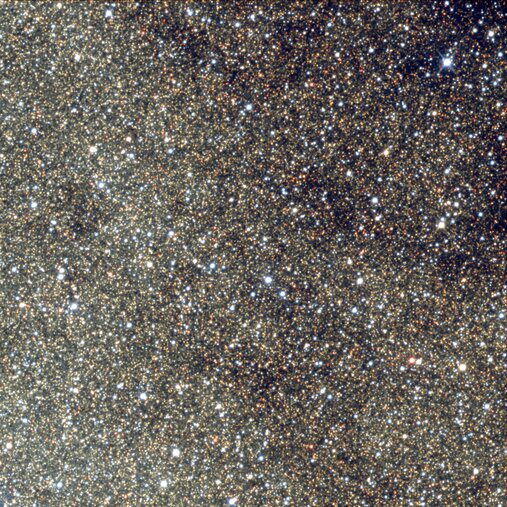
\includegraphics[width=0.5\linewidth]{../static/microlensing/crowded_field.jpg}
        \caption{
            A stellar field of a microlensing event GLE-2012-BLG-0406 (centred),
            imaged by one of Las Cumbres Observatory's 2m telescopes,
            showing the high density of stars typical in microlensing observations.
            Credit: Y. Tsapras. Taken from
            \url{http://microlensing-source.org/pictures/}.}
        \label{fig:crowded_field}
    \end{centering}
\end{figure}

That the same effect could be used to detect the presence of planets orbiting
around the lens star was first theorised by \citet{1964PhRv..133..835L}, who
wrote that \emph{``the primary effect of planetary deflectors bound to stars
    other than the Sun will be to slightly perturb the lens action of these
    stars''}. However, he was also sceptical about the possibility of detection,
saying that \emph{``associated pulses would be so weak and infrequent and of
    such fleeting duration -- perhaps a few hours -- as to defy detection''}.
Gravitational lensing as a method for discovering exoplanets really took off
with the work of Paczy\'nski
\citep{1986ApJ...304....1P,1986ApJ...301..503P,1991ApJ...374L..37M}, who also
coined the term \emph{microlensing}, referring to gravitational lensing in a
regime where the images of the background light source cannot be resolved but one can
nevertheless measure its magnification as a function of time. Microlensing as a
method for detecting exoplanets has some unique aspects. First, it is a one-off
event that happens on a timescale of a few minutes up to several months
depending on the distances to the background star, the lensing star, and the
mass of the lens. In addition to the fact that there is only one chance to
observe such an event, for it to happen at all we need extremely precise
alignment between the lens and the background star. The chance of observing
a stellar microlensing event is roughly one-in-a-million for a typical
star within the Milky Way. Observing a planetary signal is about an order of
magnitude less likely than that. Hence, obtaining a decent sample of planetary
events requires continuous monitoring on the order of $10^{8}$ stars. 
Thus, microlensing observations focus on the densest region of
the Milky Way -- the Galactic bulge. Figure~\ref{fig:crowded_field} shows a picture
of such a dense stellar field. Finally, in the vast majority of cases, we
detect no light from the lens itself. The collected photons originate from a
background star completely unrelated to and distant from the lensing star. This is
very different from other exoplanet discovery methods and means that we can only
obtain the dynamical properties of planets such as their masses and periods.


The properties of microlensing events that make them difficult to observe also mean
that they provide a unique lens on exoplanet systems. 
Relative to other methods such as transits and radial velocity, microlensing is sensitive
to planets located at substantially greater distances, well outside our
Solar System neighbourhood and even potentially to Milky Way's satellite
galaxies such as the Magellanic Clouds and the nearby Andromeda galaxy.
Microlensing is also sensitive to very small planets and planets that 
are further out from the star than those typically detected using transits and
radial velocity. Microlensing surveys such as OGLE \citep{1993AcA....43..289U}
and MOA \citep{1999PThPS.133..233M} continuously monitored crowded
stellar fields in the Milky Way since the 1990s\footnote{Initially the focus was
    on finding dark matter candidate particles -- so-called MACHOs (Massive Compact
    Halo Objects).} discovering thousands of stellar events and dozens of planetary
events. To detect planetary deviations in the observed light curve, it is
essential to have high-cadence observations of the source star. The way survey campaigns
traditionally work is that once a particular star starts to become
magnified by a large factor, many additional small telescopes join in to improve 
coverage of the key parts of the light curve. Sometimes space-based observatories 
get involved as well.
The vast majority of microlensing events analysed so far consist of
observations from multiple observatories, each with its unique aspects, such
as noise properties, cadence and photometric quality.

Future surveys such as the ground-based Rubin Observatory
\citep{2019ApJ...873..111I} telescope and the space-based Roman Telescope
\citep{2019ApJS..241....3P} and Euclid \citep{2022arXiv220209475B} will detect
tens of thousands of events in total. Although most of the microlensing literature 
is focused on characterising multiple-lens events, answering
questions about \emph{populations} of objects with these new, but also with existing datasets,
requires scalable data analysis methods and a clear set of
guidelines on how to interpret the analysis products. This is a substantial
challenge because microlensing events are notoriously difficult to model. Even
though the datasets are relatively simple (multiple time series
photometric light curves in different bands), the parameter space for even the
simplest models is highly non-linear, correlated, relatively high dimensional
and there are often near-perfect degeneracies in the solutions.
The assumptions relied on by existing methods for modelling microlensing events 
are often opaque and unquestioned. Discussions on model ``degeneracies''
\citep{2014MNRAS.437.4006S,2019AJ....157...23H,2018AcA....68...43S,2009MNRAS.393..816D},
correlated noise \citep{2015ApJ...812..136B,2019MNRAS.488.3308L}, and model
comparison \citep{2018AJ....155..259H,2019MNRAS.484.5608D}, have been ongoing in
the microlensing literature for decades without a clear solution in sight and without a proper
framing of the issue. 

In this thesis, I revisit these sorts of questions while taking into account many recent developments in the fields of
computational statistics and machine learning. 
The microlensing portion of this thesis is structured as follows. 
In Chapter~\ref{ch:caustics} I introduce the \ssf{caustics} code for computing the 
extended source magnification of single, binary, and triple-lens systems. This chapter 
deals with the \emph{forward modelling} problem of microlensing, i.e. computing the
magnification of a source star as a function of time given a set of system parameters.
The \emph{inverse problem} -- how to infer the system parameters from the observed 
light curve -- is discussed in Chapter~\ref{ch:single_lens_models} (for single lens events), 
and in Chapter~\ref{ch:multiple_lens_models} (for multiple-lens events).


\section{Occultation and phase curve mapping}
Interestingly, the history of the second topic of this thesis 
-- occultation and phase curve mapping -- is not unlike that of microlensing.
The idea of using occultations and phase curves to reconstruct a two-dimensional ``map''
of spherical astronomical bodies was proposed in the early 20th century. 
It  was only much later that technology caught up with the idea. In 1906,
\citet{1906ApJ....24....1R} pointed out that certain features in light curves
of Solar System satellites can be attributed to inhomogeneities of their
surfaces. The key idea is as follows. Although at any given time we observe only the
total light from an unresolved satellite or planet, different portions of the
surface are visible at different times. Thus, we may expect that some of the
information about the light emitted or reflected from the surface 
will be imprinted onto the light curve. 
\citet{1906ApJ....24....1R} also considered the inverse problem -- can we learn something about the surface of
these objects starting from a light curve? The method he proposed is now known
as \emph{phase curve mapping}. It was first attempted by
\citet{1972ApJ...174..449L}, who analysed photometric light curves of Pluto in
reflected light, attempting to constrain variations in the \emph{albedo} of the
surface with inconclusive results.

Later works such as
\citet{1986AJ.....92.1201D,1992Icar...97..211B,1993Icar..102..134Y,1999AJ....117.1063Y}
went a step further by using both phase curves and also light curves of
mutual \emph{occultations} of Pluto by its moon Charon to reconstruct albedo
maps of Pluto. The significant advantage of occultations relative to just
phase curves is that occultation light curves encode more information 
about the surface because the sharp limb of the occultor sweeps over the disc of
the occulted body and exposes its different parts. 
Besides Pluto, occultations of another Solar System body -- the Jovian moon Io -- 
were also analysed in the 1990s. 
Starting with the work of \citet{1994Icar..107..195S}, who observed occultations 
of Io by Europa and Jupiter, Io has been a regular target for near-infrared observations 
using ground-based telescopes such as NASA's 
Infrared Telescope Facility (IRTF). The goal of these observations is to understand 
the volcanic activity on Io's surface which is covered with many time-varying
and bright volcanic features. The observing campaign of Io has yielded insights
into the nature of its volcanic activity and it continues to this day. 

A natural question arises, can we do this with objects outside of the Solar
System? The answer is yes. \citet{2007Natur.447..183K},
\citet{2012ApJ...747L..20M}, and \citet{arXiv:1202.3829} used Spitzer
mid-infrared observations of secondary eclipses of the Hot Jupiter HD189733b
and found that surface emission is best described by the presence of a large
hot spot on the dayside of the planet longitudinally offset from the
substellar point. Similarly, \citet{2014Sci...346..838S} produced temperature
maps of the Hot Jupiter WASP-43b, \citet{2013ApJ...776L..25D} mapped the Hot
Jupiter Kepler-7b in reflected light and \citet{2016Natur.532..207D} mapped the
thermal emission from the Super Earth 55 Cancri e. These studies were able
to only capture longitudinal variations in intensity. Real exoplanet atmospheres 
are certain to have three-dimensional spatial inhomogeneities in emission more
complex than a single hot spot due to the presence of clouds, zonal jets,
storms, waves, etc. \citep{2020SSRv..216..139S}. 

In recent years there have been significant advances in the statistical modelling of
phase curves and eclipse light curves. Most notably,
\citet{2019AJ....157...64L} introduced the \ssf{starry} code which enables
analytic computation of phase curves and occultation light curves for bodies
with arbitrary emission maps expressed in a spherical harmonic basis (an idea
dating back to \citet{1906ApJ....24....1R} ). \citet{2021arXiv210306275L}
expanded the algorithm for the (considerably more complicated) case of
reflected light. In this thesis, I will present the work I have done in
collaboration with other researchers from planetary science and exoplanet
communities. I have used \ssf{starry} to map the surface of Io and investigate the
prospects for detecting fine spatial structure in the atmospheres of Hot
Jupiters using simulated JWST data. In Chapter~\ref{ch:io} I describe a  novel model for 
inferring emission maps of Io from occultation light curves. This was previously published 
in \citet{2022PSJ.....3...67B}. 
In Chapter~\ref{ch:mapping_exoplanets} I draw on the results of this work and 
investigate how feasible is it to use the same techniques in the context of 
mapping Hot Jupiter atmospheres with the goal of detecting weather and climate patterns.
The application of the occultation/eclipse mapping method to Io can be seen as the
best-case scenario for the application of the same method to exoplanets.

% CHAPTER 2: The theoretical minimum
\chapter{The theoretical minimum}
\label{ch:theoretical_min}

In this chapter, I review the basic concepts in microlensing, occultation mapping,
and computational statistics. These concepts are necessary for understanding the subsequent 
chapters.

\section{Gravitational microlensing}
\label{sec:microlensing}
Gravitational lensing is generally divided into multiple classes depending
on whether the effect is discernible at the level of individual objects or 
at a level of a statistical sample of objects. 
The primary division is between \emph{weak lensing} and \emph{strong lensing}.
The former results in a subtle distortion of the images of a background source
that can only be teased out in a statistical sense. The latter refers 
to the lensing of individual objects where the lensing effect is less subtle. 
It is further divided into
\emph{macrolensing} -- lensing of galaxies where the multiple images of the source
are resolved, and \emph{microlensing}  -- where the images are generally not resolved
and the observable is the total magnification of the source as a function of time (a light curve).
In the case of microlensing, the light source is either a quasar or a star (sometimes a binary star)
and the lenses are stars, brown dwarfs, planets, or compact objects such as black holes, neutron
stars and white dwarfs. In this thesis, I focus specifically on stellar microlensing
instead of quasar microlensing\footnote{Quasar microlensing
    is a somewhat separate community from the rest of the microlensing community.}.

\subsection{Deflection of light by gravity}
Gravitational lensing is a phenomenon fully described by Einstein's General
Theory of Relativity (GR) which predicts that light changes direction 
when passing close to a massive body. According to GR:
\begin{itemize}
    \item The presence of mass changes the spacetime geometry from the flat (Minkowski)
          metric $\eta_{\mu\nu}$ to a curved metric, specified by the tensor $g_{\mu\nu}$.
    \item Massless particles such as photons follow the null geodesics, paths we can obtain by solving the
          \emph{geodesic equation}.
\end{itemize}
If we restrict ourselves to the regime where the metric is time-independent
and the test particles are allowed to travel at any velocity less than $c$,
also known as the \emph{weak field} or \emph{linearised approximation }
of GR, the metric tensor is
\begin{equation}
    g_{\mu\nu}=\eta_{\mu\nu}+h_{\mu\nu}
    \hquad,
\end{equation}
where  (assuming that the metric sign convention is $(-,+,+,+)$ and that we are working in Cartesian coordinates
$(t, x,y,z)$) 
$h_{\mu\nu}=
    \textrm{diag}(-2\Phi,-2\Phi,-2\Phi,-2\Phi)$  \citep{carroll_2019}.
The (static) Newtonian gravitational potential $\Phi$ obeys the Poisson equation
\begin{equation}
    \nabla^2\Phi=4\pi G\rho
    \hquad,
\end{equation}
where $\rho$ is the mass density of the distribution of mass located between the observer
and the light source.

The geometry of the lensing system consists of a distant source of light, the
observer, and distribution of mass with density $\rho$ located between the
source and the observer are shown in Figure~\ref{fig:deflection_angle}.
\begin{figure}
    \centering
    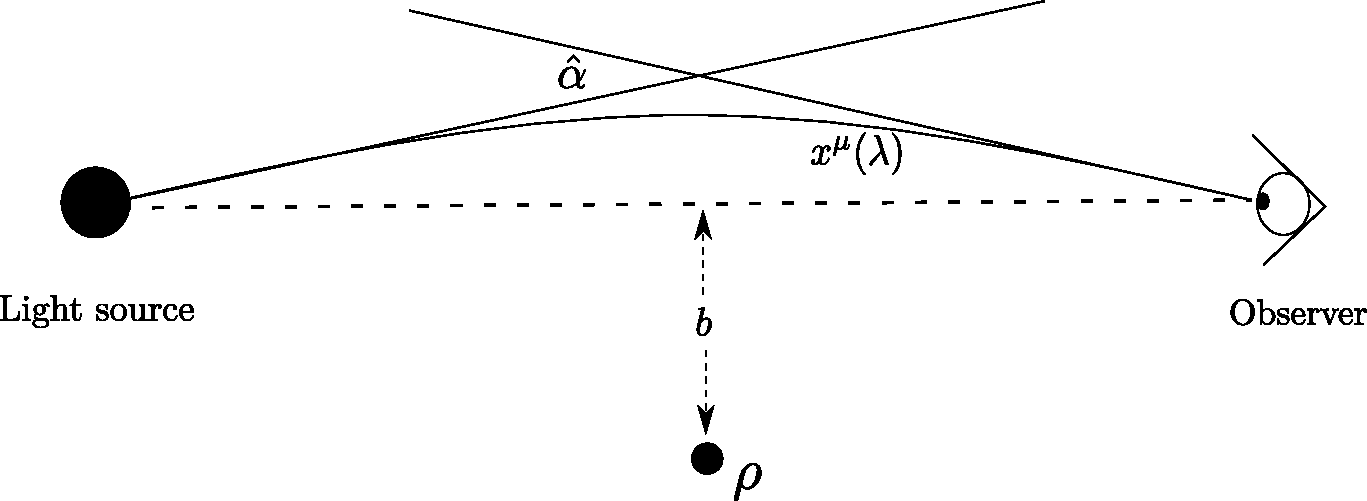
\includegraphics[width=0.6\linewidth]{../static/microlensing/deflection_angle.pdf}
    \caption{Geometry of gravitational lensing.
        A geodesic curve $x^\mu(\lambda)$ is deflected
        by an angle $\hat\alpha$ from its initial trajectory
        due to the presence of a massive body with mass density $\rho$. Figure
        adapted from \citet{carroll_2019}.}
    \label{fig:deflection_angle}
\end{figure}
A photon is deflected, as it travels from a source to an observer by a
\emph{deflection angle} $\hat\alpha$, a vector in the
plane  perpendicular to the wave vector $\vec{k}$ pointing in the direction of
photon propagation.
The deflection angle is \citep{carroll_2019}:
\begin{equation}
    \hat\alpha=2\int\nabla_\perp\Phi \ud s
    \hquad,
    \label{eq:deflection_angle_general}
\end{equation}
where $\nabla_\perp\Phi$ is the gradient of the potential in the direction transverse
to the path of the photon and $s$ is the spatial distance travelled.
For a point mass $M$, the potential is
\begin{equation}
    \Phi=- \frac{GM}{(b^2+x^2)^{1/2}}
    \hquad,
\end{equation}
where $x$ parametrises the straight line connecting the observer and the lens and
$b$ is the impact parameter of the light ray.
Integrating from $-\infty$ to $\infty$ (i.e. assuming that both
the source and the observer are located far away from the deflecting mass and that the deflection angle 
is small), we obtain
the deflection angle:
\begin{equation}
    \hat\alpha= \frac{4GM}{c^2b}= \frac{2R_s}{b}
    \hquad,
    \label{eq:deflection_angle_point_mass}
\end{equation}
where $R_s=2GM/c^2$ is the Schwarzschild radius.
$\hat\alpha$ is directly proportional to the mass of the lens and
it  is independent of the wavelength of the light. It also increases with the proximity of
the light ray to the lensing mass which is the opposite behaviour to that of a
classical convex lens for which the deflection angle vanishes at the centre of the lens.
The resulting deflection angle is very small, for example, for the Sun we have
$GM/c^2=1.48\times 10^5\si{\centi\meter}$ (2.95 km), $R=6.96\times
    10^{10}\si{\centi\meter}$ and $\hat\alpha=1.75$ arc seconds. This is the angle
that was claimed to have been observed by Eddington during the 1919 total
solar eclipse.

Equation~\ref{eq:deflection_angle_general} is valid when the linearised
approximation of GR is sufficient. In this approximation, the deflection angles
are additive, and the total deflection caused by a group of massive bodies is just
the sum of the individual deflection angles. The linearised approximation
breaks down when the impact parameter $b$ approaches the Schwarzschild radius
of the lensing mass because the linearised metric is no longer sufficient. Thus, 
except for modelling lensing in the close vicinity of a black, the linearised
approximation is adequate.

\subsection{The magnification of a point source by a point lens}
Consider a system consisting of an observer $O$, a point mass $M$, and a point
light source $S$. The geometry of this system is shown in
Figure~\ref{fig:lens_geometry}. The lens is located in the \emph{lens plane}, 
perpendicular to the observer-lens axis, at a distance $D_L$ away from
the observer. The light source is located in the \emph{source plane}
perpendicular to the observer-source axis, at a distance $D_S$ away from the
observer. The observer is in the \emph{observer plane}. The assumption that
the location of the source and the lens can be parametrised using
angular coordinates as seen by the observer (or Cartesian coordinates if the distance to the lens and
the source is known) in their respective planes is justifiable because the
deflection angles involved are tiny and the distance between the observer
and any point of interest in the lens plane is approximately constant.
\begin{figure}[!ht]
    \centering
    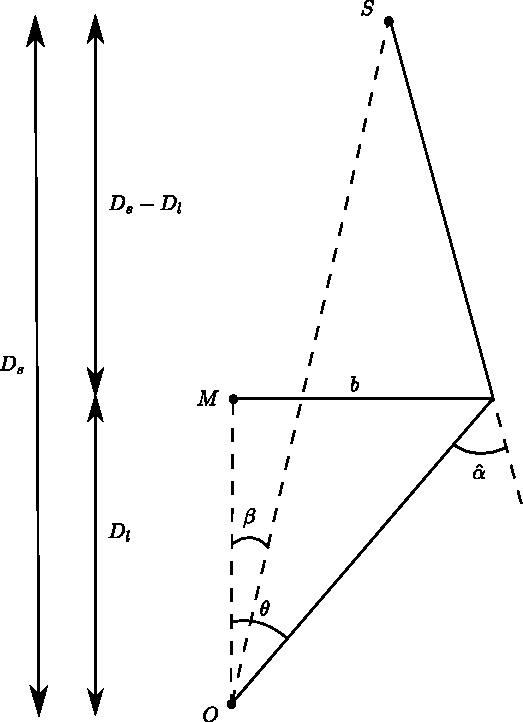
\includegraphics[width=0.4\linewidth]{../static/microlensing/lens_geometry.pdf}
    \caption{The geometry of a system consisting of a point mass lens $M$ located at a distance
        $D_L$ at angular separation $\beta$ from the observer, and a single light source $S$ 
        located at a distance $D_S$, emitting a light ray which gets
        deflected by an angle $\hat\alpha$ from its
        original trajectory. As a result, the observer sees the source at an angular separation
        $\theta$. Figure adapted from \citet{1992grle.book.....S}.}

    \label{fig:lens_geometry}
\end{figure}
Let $\theta$ be the apparent angular position of the source in the sky with respect to the
observer--lens axis and $\beta$ be the actual angular position of the source.
Assuming a metric for spacetime in between the source and the observer that is
approximately Euclidian\footnote{Which is a valid assumption for galactic sources but not for
    extragalactic sources such as quasars and galaxies require a cosmological
    model for the metric.} the distance from the lens to the
source is $D_S-D_L$.

From Figure~\ref{fig:lens_geometry} and using Equation~\ref{eq:deflection_angle_general} it follows 
that the relationship between
the observed and the actual location of the source is 
\begin{equation}
    \beta=\theta-2 R_s \frac{D_S-D_L}{D_LD_S}
    \frac{1}{\theta}
    \hquad,
    \label{eq:lens_equation}
\end{equation}
which is known as the \emph{lens equation} or sometimes also the \emph{ray-tracing}
equation. If the source and the lens are perfectly aligned with respect to the observer,
then $\beta=0$ and $\theta\equiv\theta_E$ where
\begin{equation}
    \theta_E= \sqrt{ \frac{4GM}{c^2} \left( \frac{1}{D_L} - \frac{1}{D_S} \right)}=
    \sqrt{\kappa M\pi_{LS}}
    \hquad,
    \label{eq:angular_einstein_radius}
\end{equation}
where $\kappa \equiv \frac{4 G}{c^{2} \mathrm{au}} \simeq 8.1 \frac{\mathrm{mas}}{M_{\odot}}$
and
\begin{equation}
    \pi_{LS}\equiv\pi_L - \pi_S=\frac{1\mathrm{au}}{D_L}-\frac{1\mathrm{au}}{D_S}
\end{equation}
is the relative lens-source parallax.

With perfect alignment ($\beta=0$), the image of the source forms a ring (the Einstein ring) around the lens star
with angular radius $\theta_E$ -- the \emph{Einstein radius}. $\theta_E$
depends on the mass of the lens and the distances to the lens and the source.
The angular Einstein radius sets the characteristic scale of a microlensing
event; it is a natural unit for most microlensing parameters. For an M-dwarf
star lens in the galactic disc ($D_L\sim 3\,\textrm{kpc}$) and a source star in
the galactic bulge ($D_S\sim 8\,\textrm{kpc}$) we have $\theta_E\sim
    1\,\textrm{mas}$ so the typical scale of microlensing is on the order of
milliarcseconds. The images of the source star are only rarely observable using
the most advanced optical interferometers, such as the GRAVITY instrument on
ESO's Very Large Telescope, whose lower resolution limit is $2\,\textrm{mas}$
\citep{arXiv:1705.02345}. \citet{2019ApJ...871...70D} were the first to resolve
the images of a microlensing event, finding the value of
$\theta_E=1.87\,\textrm{mas}$ using the GRAVITY instrument.

We can rewrite Equation~\ref{eq:lens_equation} by defining new dimensionless
angular coordinates scaled by the angular Einstein radius:
\begin{equation}
    z\equiv \frac{\theta}{D_L\theta_E}, \quad w\equiv\frac{\beta}{D_S\theta_E}
    \hquad.
\end{equation}
The lens equation then takes the very simple form
\begin{equation}
    z= w- \frac{ 1}{w}
    \hquad.
    \label{eq:lens_equation_dimensionless}
\end{equation}
Equation~\ref{eq:lens_equation_dimensionless} is a non-linear mapping between the
source plane $w$ and the lens plane $z$.
If we solve for $z$, we obtain two solutions for the position of the images, given by
\begin{equation}
    z_\pm= \frac{1}{2} \left( w\pm\sqrt{w^2 +4}\right)
    \hquad.
    \label{eq:images_location}
\end{equation}
For non zero $w$, the so-called \emph{minor image} is always located
within the Einstein radius ($\lvert z_-\rvert<1$) while the \emph{major image}
is located outside of it ($\lvert z_+\rvert>1$).

Because gravitational lensing involve no additional emission or
absorption along a deflected ray of light and the there is no net wavelength shift 
between the emission point and the observer,  the \emph{surface brightness}
(flux density per unit angular area), $I$, of the source image is identical to
the surface brightness of the unlensed source. The flux of an infinitesimal
source is a product of the surface brightness and the solid angle $\Delta
    \omega$ subtended by the source in the sky. 
    This flux changes throughout the
microlensing event because the source and the lens are in motion relative to an
observer. The ratio of the original and the lensed source flux, the
\emph{magnification} $A$, is then: 
\begin{equation}
    A= \frac{\Delta \omega}{(\Delta\omega)_0}\hquad,
    \label{eq:magnification}
\end{equation}
where $0$ denotes the unlensed solid angle.
Assuming that the source has infinitesimal size and is at an angular location
$\mathbf w \equiv (w_1,w_2)$ subtending an angle
$\Delta (\omega)_0$, and an image of the source at location
$\mathbf z\equiv(z_1,z_2)$ subtending an angle
$\Delta \omega$; the ratio between the solid angle of the source and the image
is given by the determinant of the Jacobian matrix of the
lens mapping $\mathbf{z}\rightarrow\mathbf{w}$, evaluated at the location of
the images
\begin{equation}
    \frac{(\Delta\omega)_0}{\Delta\omega} =\left\lvert\textrm{det}
    \frac{\partial \mathbf w}{\partial \mathbf z} \right\rvert
    \hquad.
\end{equation}
The magnification $A$ is then given by the inverse Jacobian determinant
of the lens mapping:
\begin{equation}
    A= \left\lvert\det
    \frac{\partial \mathbf w}{\partial \mathbf z} \right\rvert^{-1} 
    \hquad.
    \label{eq:magnification_general}
\end{equation}
The images for which the determinant of the Jacobian of the lens mapping is
positive are said to have positive \emph{parity} and vice versa.

Looking at Equation~\ref{eq:magnification_general}, we see that the
magnification diverges when the Jacobian determinant of the lens mapping
vanishes. Curves in the lens plane for which the determinant of the lens
mapping vanishes, that is,
\begin{equation}
    \left\lvert\det
    \frac{\partial \mathbf w}{\partial \mathbf z} \right\rvert=0
    \hquad,
\end{equation}
are called \emph{critical curves}.
The critical curves in the lens plane can be mapped to the source plane using
the lens equation $\mathbf{z}\rightarrow \mathbf{w}$, and these curves 
are called \emph{caustic curves}.
Although the magnification factor in Equation~\ref{eq:magnification_general} formally
diverges at the points of critical curves or caustics,
the divergence is not physical because light sources are not in reality point-like.
If the finite angular size of the source is taken into
account, the magnification is an integral of Equation~\ref{eq:magnification_general} over the
the extent of the source, weighted by the source brightness and that integral is always finite.
The critical and caustic curves are closed curves and one show that \emph{the
    number of images changes by two if and only if the source crosses a caustic curve}
\citep[][Chapter 6]{1992grle.book.....S}.

We can derive a simpler expression for Equation~\ref{eq:magnification} by
switching to polar coordinates $(v,\phi)$ in the lens plane. The lens equation
for the two vector components of the apparent source position is 
\begin{align}
    w_1= & z_1- \frac{z_1}{z_1^2+z_2^2} \\
    w_2= & z_2- \frac{z_2}{z_1^2+z_2^2}
    \hquad.
\end{align}
Introducing polar coordinates $z_1=v\cos\phi,\;z_2=v\sin\phi$, we have
\begin{equation}
    \left\lvert\textrm{det}
    \frac{\partial \mathbf w}{\partial \mathbf z} \right\rvert =1- \frac{1}{v^4}
    \hquad.
\end{equation}
By substituting the locations of the source images
Equation~\ref{eq:images_location} into the
above expression, we obtain the magnification of the source images
\begin{equation}
    A_\pm = \frac{1}{2}\left(\frac{u^{2}+2}{u \sqrt{u^{2}+4}} \pm 1\right)
    \hquad,
    \label{eq:magnification_per_image}
\end{equation}
where $u = \sqrt{w_1^2+w_2^2}$ is the magnitude of the position
vector of the source star.
The total magnification is then the sum of the two magnifications and is given by
\citep{1936Sci....84..506E}
\begin{equation}
    A(u)=\lvert A_-\rvert+\lvert A_+\rvert= \frac{u^2+2}{u\sqrt{u^2+4}}
    \hquad,
    \label{eq:magnification_point_lens}
\end{equation}
For a single point lens, the critical curve is simply the Einstein
ring corresponding to $v=\sqrt{z_1^2+z_2^2}=1$, and the caustic curve is mapped to 
a single point in the source plane at $u=0$.
For source separations much smaller than the angular Einstein radius ($u\ll 1$), the
magnification is approximately $A(u)\simeq 1/u$. In the opposite case ($u\gg 1$)
we have $A(u)\simeq 1+ 2/u^4$, that is, the magnification falls off rapidly the further
away the source is from the lens.

To evaluate Equation~\ref{eq:magnification_point_lens} in practice,
we have to parametrise the position of the source on the sky $u$ as a function
of time. To derive an expression for $u(t)$, we assume that the motion of the
observer, the lens, and the source is rectilinear (acceleration is neglected).
We take $\vec{w}_S$ to be the angular position of the source star on the plane
of the sky and $\boldsymbol{\mu}_L$ to be its proper motion vector. Likewise,
for the lens. We thus have:
\begin{align}
    \vec{w}_S(t) & =\vec{w}_{S, 0}+
    \left(t-t_{0}\right) \boldsymbol{\mu}_S
    \label{eq:source_position}      \\
    \vec{w}_L(t) & =\vec{w}_{L, 0}
    +\left(t-t_{0}\right) \boldsymbol{\mu}_L
    \hquad,
    \label{eq:lens_position}
\end{align}
where $t_0$ is some reference time.
The relative position vector of the lens with respect to the source is then
\begin{equation}
    \boldsymbol{u}(t) \equiv \frac{\vec{w}_L(t)
        -\vec{w}_S(t)}{\theta_E}=
    \frac{\vec{w}_{LS, 0}}{\theta_E}
    +\frac{t-t_{0}}{\theta_E} \boldsymbol{\mu}_{LS}
    \hquad,
    \label{eq:relative_trajectory_no_parallax}
\end{equation}
where
$\vec{w}_{L S, 0}\equiv\vec{w}_{L,0}-\vec{w}_{S, 0}$
is the relative position at $t_0$, and
$\boldsymbol{\mu}_{LS}\equiv \boldsymbol{\mu}_{L}- \boldsymbol{\mu}_{S}$ is the
relative proper motion.
Since $\boldsymbol{\mu}_{LS}$ and $\vec{w}_{L S, 0}$ are
perpendicular to each other, it follows that the magnitude of the relative
separation is
\begin{equation}
    u(t)=\sqrt{u_0^2+ \left(\frac{t-t_0}{t_E}\right)^2}
    \hquad,
\end{equation}
where we have defined $u_0\equiv |\vec{w}_{L S, 0}|/\theta_E$
and $t_E\equiv \theta_E/|\boldsymbol{\mu}_{LS}|$.
The magnification is a function of three parameters $(t_0, u_0, t_E)$,
and the resulting curve as a function of time is often called the Paczy\'nski curve
\citep{1986ApJ...304....1P,1986ApJ...301..503P}.
The magnification as a function of time for different impact parameters $u_0$
is shown in Figure~\ref{fig:paczynski_curve}. Notice the very steep fall-off in
magnification as we move away from the Einstein ring ($A(u)\propto
    1+2u^{-4}$).
In the limits of $u_0\rightarrow 0$ and $u_0\gg 1$  there is a continuous
mathematical degeneracy between the parameters $t_0$, $u_0$ and $t_E$
\citep{1997ApJ...487...55W}.

\begin{figure}[t]
    \begin{centering}
        \includegraphics[width=0.7\linewidth]{figures/paczynski_curve.pdf}
        \caption{
            Magnification of a point source by a point lens as a function of time. The
            various magnification curves correspond to different impact parameters $u_0$.
            The inset figure
            shows the source trajectories in the lens plane, the dashed circle corresponds
            to the Einstein radius $v=1$.}
        \label{fig:paczynski_curve}
        \script{chapter_2/paczynski_curve.py}
    \end{centering}
\end{figure}

\subsection{Observed flux}
The magnification $A(t)$ is not a direct observable in microlensing events. We
can measure the flux of the source star, which is usually contaminated by 
the flux of other nearby stars and potentially also
with light from the lens and possible companions to the lens. The observed flux
is then
\begin{equation}
    F(t)=F_S\,A(t)+F_B
    \hquad
    \label{eq:flux_observed_micro}
\end{equation}
where $F_S$ is the flux of the source star and $F_B$ is the contamination flux, also
called the \emph{blending flux}. To quantify the strength of the blending, we can also
define the \emph{source flux fraction} $b_S$ as the fraction of total (unmagnified)
flux that is coming from the source star:
\begin{equation}
    b_S\equiv F_S/(F_S + F_B)
    \hquad.
\end{equation}
For highly blended events $b_S\approx 0$ and in the absence of blending $b_S=1$.
The source flux $F_S$ and the blending flux $F_B$ are generally highly correlated,
and it is sometimes preferable to use a slightly different parametrisation proposed by
\citet{2009MNRAS.393..816D}. In this parametrisation, we use the
\emph{baseline flux} $F_\mathrm{base}$ and the difference between
the baseline flux and the flux at peak magnification $\Delta F\equiv F_S[A(u_0)-1]$
as the new parameters.
Equation~\ref{eq:flux_observed_micro} then takes the form
\begin{equation}
    f=\Delta F\frac{A(t) - 1}{A(t_0)-1}+F_\mathrm{base}
    \hquad.
    \label{eq:flux_dominik}
\end{equation}
It is generally straightforward to measure the flux difference $\Delta F$, the
baseline flux $F_\mathrm{base}$ and the centre of the curve $t_0$ but getting a
good estimate of $t_E$ even outside of the regime $u_0\rightarrow 0$ and
$u_0\gg 1$ requires good photometric sampling along the ``wings'' of the light
curve \citep{2009MNRAS.393..816D}.
Although the parametrisation defined in Equation~\ref{eq:flux_dominik} best maps to 
the observable features in the light curve, I prefer to use the parametrisation which 
uses the parameters $(F_S,F_\mathrm{base})$:
\begin{equation}
    f=F_S\left[A(t) - 1\right]+F_\mathrm{base}
    \hquad.
    \label{eq:lin_flux_parameters}
\end{equation}
The advantage of this parametrisation is that it still uses the baseline flux 
$F_\mathrm{base}=F_S+F_B$ which is a direct observable, but it does not require an extra evaluation 
of the magnification $A(t_0)$. In addition, $F_S$ is a parameter for which it easier to 
set a sensible prior.
As we shall see in Section~\ref{ssec:marginalise_linear}, the choice of parametrisation in
this case is not so important because in end the we will always marginalise (integrate out)
the linear parameters.

\subsection{Astrometric microlensing}
\label{ssec:astrometric_microlensing}
\begin{figure}[t]
    \begin{centering}
        \includegraphics[width=0.7\linewidth]{figures/single_lens_astrometric_shift.pdf}
        \caption{
            The astrometric shift in the centroid of light for a point source point lens
            model.
            The various curves correspond to different impact parameters $u_0$.}
        \label{fig:single_lens_astrometric_shift}
        \script{chapter_2/single_lens_astrometric_shift.py}
    \end{centering}
\end{figure}

In addition to the photometric microlensing effect, there is also the astrometric
microlensing effect. Astrometric microlensing refers to the relative shift in 
the \emph{angular position} of the unmagnified source star when it is in the vicinity of the lens.
For a point source and a single lens, we can
define the light centroid of the two images by weighting their positions
(Equation~\ref{eq:images_location}) with their magnifications
(Equation~\ref{eq:magnification_per_image}):
\begin{equation}
    \vec z_\mathrm{cent}=\frac{A_+\vec z_+ + A_-\vec z_-}{A_+ + A_-}
    \hquad,
    \label{eq:centroid_single_lens}
\end{equation}
where $\vec z_\mathrm{cent}$ is the position of the centroid. It follows that the magnitude of the
shift is
\begin{equation}
    z_\mathrm{cent}=\frac{1}{2}\left(\frac{u(u^2 + 4)}{u^2+2}+u\right)
    \hquad,
\end{equation}
and the magnitude $\delta z_\mathrm{cent}$ of the shift
$\delta \vec z_\mathrm{cent}\equiv\vec z_\mathrm{cent} - \vec u$ relative to the source star is
\begin{equation}
    \delta z_\mathrm{cent} = \frac{u}{u^2 + 2}
    \hquad.
\end{equation}
Figure~\ref{fig:single_lens_astrometric_shift} shows the centroidal shift for
different values of the impact parameter $u_0$. The trajectories trace out ellipses
\citep{1995ApJ...453...37W}.
Whereas the photometric effect is
strongest for
$u\ll 1$, the astrometric shift peaks at $u=\sqrt{2}$ with
$\delta z_{\mathrm{cent},\max}\approx 0.354$ in units of the angular Einstein radius.
Importantly, the astrometric shift falls off as $1/u$ for $u\gg \sqrt{2}$, which is
much slower than $A\propto 1/u^4$ for the photometric effect.
In this thesis I focus exclusively on the photometric microlensing effect, although many 
of the methods I develop in later chapters are also applicable to astrometric microlensing.

\subsection{Magnification of an extended source}
\begin{figure}[t]
    \begin{centering}
        \includegraphics[width=\linewidth]{figures/single_lens_images.pdf}
        \caption{Images of an extended limb-darkened source star lensed by a single
            point lens for varying positions of the source star. The top panels show the magnification map with a logarithmic scale
            colourmap  consisting of a single-point caustic. The semi-transparent circle
            is the source star disc with radius $\rho_\star=0.15$. The bottom row shows
            the two images merging into the Einstein ring as the source moves over the caustic.}
        \label{fig:single_lens_images}
        \script{chapter_2/single_lens_images.py}
    \end{centering}
\end{figure}
For a relatively small subset of microlensing events, the source star passes
very near to the caustic. 
As a result,  the change in magnification over the extent of
the source star disc with radius $\theta_\star$ is non-negligible and the point source
approximation breaks down. 
This breakdown will generally happen when $u_0 \lesssim
    \rho_\star/2$ \citep{1997ApJ...477..580G}, where
$\rho_\star=\theta_\star/\theta_E$. The effect of finite source effects on the
magnification curve thus matters only near the peak of an event.
It results in a rounder peak of the light curves shown in Figure~\ref{fig:paczynski_curve}.

There are no analytic solutions for the magnification of an
extended source magnified by a single point lens with a general surface brightness
profile. \citet{1994ApJ...421L..71G} derived an approximate solution valid for
uniform brightness sources with $\rho_\star\lesssim 0.1$, and
\citet{1994ApJ...430..505W} derived a general solution (also for a uniform
brightness source) involving solutions to elliptic integrals of the first,
second and third kinds. \citet{2009ApJ...695..200L} proposed a simple method for
numerically integrating the point source magnification over the extent of the source
disc, which is fast and accurate for arbitrary intensity profiles.
Another solution involving fast Fourier transforms any source profile was
recently proposed by \citet{2022arXiv220306637S}.

To illustrate the microlensing of an extended source,
in Figure~\ref{fig:single_lens_images} I plot the magnification map and the
images of an extended limb-darkened source (with $\rho_\star=0.15$) as it
approaches the point caustic for a single lens. The top panels in the figure show the
magnification map in the source plane with a logarithmic scale colourmap. The
source disc (semi-transparent grey circle) is shown at different positions
relative to the caustic. The bottom panels show the resulting images in the
image plane, which is what we would see in the sky if we could resolve the
microlensing event. As the source moves closer to the caustic, the area (and
hence the magnification) of the two images increases, and eventually,  they merge
and form an Einstein ring.

To produce these plots, I evaluated the lens mapping
(Eq.~\ref{eq:lens_equation_dimensionless}) on a regular grid in the image plane
and then plotted the surface brightness of the corresponding point on the
source disc in the source plane. I will discuss all of this in far greater
detail In Chapter~\ref{ch:single_lens_models} but, for now, I should mention a
few key points:
\begin{itemize}
    \item Every point inside the two images maps to a single point on the source disc via
          the lens equation. The inverse mapping is one-to-many because each point on the
          source disc maps to two points (point lens images) in the image plane. The
          points on the limbs of the two physical images correspond to points on the limb of
          the source disc. We cannot predict the location of the images without inverting
          the lens mapping
    \item To compute the magnification of an extended source numerically, we can either
          integrate the magnification function convolved with the source brightness
          profile over the entire source disc (a two-dimensional integral), or we can 
          do the same integral in the image plane. The first approach is 
          numerically unstable because we would need to integrate over a function which
          diverges as $1/r$ approaching the caustic. This would require a very large
          number of lens equation evaluations. Hence it is preferable to integrate in
          the image plane where the function is smooth.
    \item Decreasing the source radius $\rho_\star$ results in narrower arcs of the
          images with smaller radial and azimuthal extent.
\end{itemize}
In Chapter~\ref{ch:caustics} I discuss how things change for binary and triple lens 
systems where the caustics are much more complex.

\subsection{Annual parallax}
\label{ssec:single_lens_parallax}
In Equation~\ref{eq:relative_trajectory_no_parallax} we have assumed that the
the relative motion of the lens with respect to the source on the plane of the sky
is rectilinear.
This is a reasonable approximation in a barycentric frame of
reference if the acceleration of the source and the lens can be neglected.
However, the majority of microlensing events are observed from a non-inertial geocentric
frame (Earth) and sometimes from multiple locations simultaneously. In those
cases, we have to take into account parallax effects.
We differentiate between two kinds of parallax. 

The first kind is the \emph{annual
    parallax} (sometimes also called the orbital parallax). 
It is the change in the  
lens-source relative motion vector $\boldsymbol\mu_{LS}$ due to the local
acceleration of Earth in its orbit. Annual parallax is important for long-timescale events
when the event timescale is equal to some substantial fraction of a year. The
effect of annual parallax is usually a slight modification of the shape of the
classic Paczy\'nski curve.
The second kind of parallax is the \emph{satellite parallax} which refers to the
difference in viewpoint if we have simultaneous observations of the source
star from different locations which are separated by a substantial fraction of the
Einstein ring projected onto the observer plane $\tilde{r}_E\equiv
    D_{LS}\theta_E$ (where $D_{LS}^{-1}=D_L^{-1} - D_S^{-1}$). In practice, this
means simultaneously observing a microlensing event from Earth and a space-based telescope.
It was first proposed by \citet{1966MNRAS.134..315R}. There is
also the ``terrestrial parallax'', which is identical to the satellite parallax
except that it involves only ground-based observations separated by a significant 
fraction of Earth's diameter. Measurement of these parallax effects allows
for a partial breaking of the degeneracy in the event timescale $t_E$ by
providing a relationship between the mass and the distance to the lens
(assuming one can estimate the distance to the source star).

In this section, I will describe the annual parallax effect because it is most relevant
for this thesis. We start by
modifying Equations~\ref{eq:source_position} and \ref{eq:lens_position} to
include the projected motion of the Sun relative to the Earth on the plane of
the sky. We project $\mathbf s(t)$ -- the position vector of the Sun relative to
Earth, onto a plane perpendicular to the line of sight towards the source star
(plane of the sky), which is defined by the unit vector $\boldsymbol{\hat n}$
normal to the plane. This geocentric coordinate system is defined at some reference time
$t_0^\prime$.  The unit vector $\boldsymbol{\hat n}$ depends on the sky
coordinates of the source star $(\alpha,\delta)$ (right ascension and
declination). We work in geocentric equatorial coordinates defined by
the spherical unit vectors $\hat{\mathbf e}_n$, which points North, and
$\hat{\mathbf e}_e$ pointing eastward such that the coordinate system is
right-handed. The unit vectors are defined by
\begin{align}
    \hat{\mathbf e}_e & = \hat{\mathbf z}\times \hat{\mathbf n}  \\
    \hat{\mathbf e}_n & = \hat{\mathbf n}\times\hat{\mathbf e}_e
    \hquad.
\end{align}
The two components of $\mathbf s$ projected onto the plane of the sky are then
\begin{align}
    \zeta_E(t;\alpha,\delta)&\equiv \mathbf s\cdot \hat{\mathbf e}_e
    \label{eq:zeta_E_t}\\
    \zeta_N(t;\alpha,\delta)&\equiv \mathbf s\cdot \hat{\mathbf e}_n
    \hquad.
    \label{eq:zeta_N_t}
\end{align}
In practice, we can retrieve $\mathbf{s}(t)$ using NASA's JPL Horizons system and compute
the projected separation at any time $t$. 
The angular positions of the source and the lens
(Equations~\ref{eq:source_position} and \ref{eq:lens_position}) then become
\begin{align}
    \vec{w}_S(t) & = \vec{w}_{S,0}+(t-t_0^\prime)\boldsymbol{\mu}_S
    +\pi_S\,\boldsymbol{\zeta}(t)                            \\
    \vec{w}_L(t) & = \vec{w}_{L,0}+(t-t_0^\prime)\boldsymbol{\mu}_L
    +\pi_L\,\boldsymbol{\zeta}(t)
    \hquad,
\end{align}
where  $\pi_S\equiv 1\,\mathrm{au}/D_S$ is the source parallax, and $\pi_L$ is the
lens parallax.
The relative separation is 
\begin{equation}
    \boldsymbol{u}(t)= \frac{\vec{w}_{LS, 0}}{\theta_E}
    +\frac{t-t_0^\prime}{\theta_E}\boldsymbol{\mu}_{LS}+\pi_{E}\,\boldsymbol{\zeta}(t)
    \hquad,
    \label{eq:relative_separation_parallax}
\end{equation}
where
\begin{equation}
    \pi_E\equiv \frac{\pi_{LS}}{\theta_E}
    \hquad.
    \label{eq:pi_E}
\end{equation}

Since annual parallax is a higher-order effect affecting the apparent
trajectory of the source on the sky that is often not very well constrained by the data, 
it makes sense to decompose the trajectory as a sum of rectilinear motion plus a deviation 
due to parallax
\citep{2002ApJ...572..521A,2004ApJ...606..319G}. In other words, we can write 
\citep{2002ApJ...572..521A}
\begin{align}
    \vec{u}(t_0^\prime)&\equiv \vec{u}_0=\vec{w}_{LS}/\theta_E+\pi_E\vec{\zeta}(t_0^\prime)\\
    \dot{\vec u}(t_0^\prime)&\equiv \dot{\vec u}_0=\vec{\mu}_{LS}+\pi_E\dot{\vec{\zeta}}(t_0^\prime)
    \hquad.
\end{align}
Combining the above definitions with Equation~\ref{eq:relative_separation_parallax}, we obtain
\begin{equation}
    \boldsymbol{u}(t)=\mathbf{u}(t_0^\prime) + (t-t_0')\,\dot{\vec{u}}(t_0^\prime) +
    \pi_E\,\delta\vec\zeta(t)
    \hquad,
\end{equation}
where 
\begin{equation}
    \delta\boldsymbol \zeta (t)=\boldsymbol \zeta (t)-\boldsymbol \zeta (t_0')-(t-t_0')
    \boldsymbol{\dot \zeta} (t_0')
    \label{eq:relative_separation_parallax_decomposed}
\end{equation}
is the position offset of the Sun on the plane of the sky relative to its position 
at the reference time $t_0^\prime$. By construction, we have 
$\delta\boldsymbol \zeta (t_0')=0$ and $\delta\dot{\boldsymbol \zeta} (t_0')=0$.
At the reference time $t_0^\prime$, the vectors $\vec{u}(t_0^\prime)$ and 
$\dot{\vec u}(t_0^\prime)$ are perpendicular to each other.

\subsubsection{$\mathbf{u}(t)$ in the $(\mathbf{\hat e}_\bot,
        \mathbf{\hat e}_\parallel)$ coordinate system}%

\begin{figure}
    \centering
    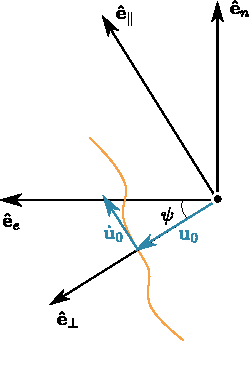
\includegraphics[width=0.3\linewidth]{../static/microlensing/microlensing_parallax_coordinates.pdf}
    \caption{A coordinate system
        $(\mathbf{\hat e}_\bot,\mathbf{\hat e}_\parallel)$ parallel to the source trajectory at time $t_0$. The orange curve
        represents the source trajectory relative to the lens at the origin. The
        coordinate system $(\mathbf{\hat e}_\bot,\mathbf{\hat e}_\parallel)$ is related to the equatorial coordinates $(\mathbf{\hat
                e}_e,\mathbf{\hat e}_n)$ by a rotation through an angle $\psi$.}
    \label{fig:parallax2}
\end{figure}

To evaluate Equation~\ref{eq:relative_separation_parallax_decomposed}, we need
to choose a suitable basis. A natural coordinate system for describing the
trajectory of the source relative to the lens is one defined by unit vectors
$(\mathbf{\hat e}_\bot,\mathbf{\hat e}_\parallel)$ where $\mathbf{\hat e}_\parallel$ 
is parallel to the trajectory $\mathbf{u}(t)$ at time $t_0^\prime$
(Figure~\ref{fig:parallax2}). 
We define the unit vectors as
\begin{equation}
    \mathbf{\hat e}_\bot\equiv \frac{\mathbf{u}_0}{|\mathbf{u}_0|}\quad,
    \mathbf{\hat e}_\parallel\equiv \frac{\mathbf{\hat n}\times\mathbf{u}_0}{|\mathbf{u}_0|}\quad
    \hquad.
\end{equation}
The coordinate system $(\mathbf{\hat e}_\bot,\mathbf{\hat e}_\parallel)$ is related to 
ecliptic coordinates by a simple rotation through an angle $\psi$
\begin{equation}
    \begin{pmatrix}
        \mathbf{\hat e}_\bot \\
        \mathbf{\hat e}_\parallel
    \end{pmatrix}
    =
    \begin{pmatrix}
        \cos\psi & -\sin\psi \\
        \sin\psi & \cos\psi
    \end{pmatrix}
    \begin{pmatrix}
        \mathbf{\hat e}_e \\
        \mathbf{\hat e}_n
    \end{pmatrix}
    \label{eq:ecliptic_to_parallel}
    \hquad.
\end{equation}
By construction, at time $t_0^\prime$ we have
$\mathbf{u}_0\,\bot\,\dot{\mathbf{u}}_0$ so the two components of
$\mathbf{u}(t)$ are then:
\begin{align}
    u_\bot(t)      & \equiv \mathbf{u}(t)\cdot \mathbf{\hat e}_\bot= u_0 +
    \pi_E\,\delta\boldsymbol \zeta(t)\cdot\mathbf{\hat e}_\bot                                                                                                                                       \\
    u_\parallel(t) & \equiv \mathbf{u}(t)\cdot \mathbf{\hat e}_\parallel= (t-t_0^\prime)\,\dot{\mathbf{u}}_0\cdot\mathbf{\hat e}_\parallel+ \pi_E\,\delta\boldsymbol \zeta(t)\cdot\mathbf{\hat e}_\parallel
    \hquad.
\end{align}
Using the definitions of the unit vectors and
$\delta\boldsymbol \zeta(t)=
    \delta \zeta_E(t)\,\mathbf{\hat e}_e+\delta \zeta_N(t)\,\mathbf{\hat e}_n$, we have
\begin{align}
    u_\bot(t)      & = u_0 + \pi_E\,\cos\psi\,\delta \zeta_E(t) - \pi_E\,\sin\psi\,\delta \zeta_N(t)
    \label{eq:u_t_parallel1}                                                                         \\
    u_\parallel(t) & =(t-t_0^\prime)/t_E^\prime + \pi_E\,\sin\psi\,\delta \zeta_E(t) +
    \pi_E\,\cos\psi\,\delta \zeta_N(t) \label{eq:u_t_parallel2}
    \hquad,
\end{align}
where $t_E^\prime \equiv|\dot{\mathbf{u}}_0|=|\boldsymbol\mu_{LS}/\theta_E  + \pi_E\,\dot{\boldsymbol \zeta}(t_0^\prime)|$.
The model parameters that determine the magnification $A(t)$ are 
$\left(u_0,t_0^\prime,t'_E,\pi_E,\psi\right)$. Notice that in this case, $u_0$
can be negative.

An alternative parametrisation which is more commonly used in the literature is obtained by
defining components of a ``microlensing parallax vector'' as
\begin{align}
    \pi_{E,N} & \equiv \pi_E\cos\psi \\
    \pi_{E,E} & \equiv \pi_E\sin\psi
    \hquad,
\end{align}
in which case we have
\begin{align}
    u_\bot(t)      & = u_0 + \pi_{E,N}\,\delta \zeta_E(t) - \pi_{E,E}\,\delta \zeta_N(t) \\
    u_\parallel(t) & =(t-t_0^\prime)/t_E^\prime + \pi_{E,E}\,\delta\zeta_E(t) +
    \pi_{E,N}\,\delta\zeta_N(t)
    \hquad,
\end{align}
and the model parameters are $\left(u_0,t_0^\prime,t_E^\prime,\pi_{E,E},\pi_{E,N}\right)$.

For reference, we can also write down the components of $\mathbf{u}(t)$ in
equatorial coordinates by inverting the rotation matrix in
Equation~\ref{eq:ecliptic_to_parallel} and applying it to
Equations~\ref{eq:u_t_parallel1} and \ref{eq:u_t_parallel2}. 
The two components are 
\begin{align}
    u_e & =u_0\cos\psi + (t-t_0^\prime)/t_E^\prime\sin\psi + \pi_E\,\delta\zeta_E(t)  
    \label{eq:u_t_east}\\
    u_n & =-u_0\sin\psi + (t-t_0^\prime)/t_E^\prime\cos\psi + \pi_E\,\delta\zeta_N(t)
    \hquad.
    \label{eq:u_t_north}
\end{align}

\subsubsection{$\mathbf{u}(t)$ in the $(\mathbf{\hat e}_\parallel, \mathbf{\hat e}_\bot)$ coordinates using acceleration parameters} 
There exists another parametrisation of the trajectory in which we fit for the local
acceleration of the lens at $t_0^\prime$ instead of $\pi_E$ and the angle $\psi$. 
I derive it here for completeness.
We define the position, velocity and acceleration such that at $t=t_0^\prime$ we have
\begin{align}
    \mathbf{u}(t_0^\prime)       & \equiv \widetilde{u}_0 \,\hat{\mathbf e}_\bot
    \label{eq:u_primed_def}                                               \\
    \dot{\mathbf{u}}(t_0^\prime) & \equiv \frac{1}{\widetilde{t_E^\prime}}\,
    \hat{\mathbf e}_\parallel \label{eq:u_dot_primed_def}                 \\ \ddot{\mathbf{u}}(t_0^\prime) & \equiv
       a_\bot\,\hat{\mathbf e}_\bot + a_\parallel\,\hat{\mathbf e}_\parallel \label{eq:u_ddot_primed_def}
       \hquad,
\end{align}
where $a_\parallel$ and $a_\bot$ are the two components of the instantaneous acceleration of
the lens at $t_0^\prime$. From Equations~\ref{eq:u_t_parallel1} and
\ref{eq:u_t_parallel2} it follows that
\begin{align}
    \mathbf{u}(t_0^\prime)       & = u_0\,\hat{\mathbf e}_\bot                    \\
    \dot{\mathbf{u}}(t_0^\prime) & =\frac{1}{t_E^\prime}\,\hat{\mathbf e}_\parallel     \\ \ddot{\mathbf{u}}(t_0^\prime) &
       =\left[\pi_E\cos\psi\,\delta\ddot{\zeta}_e(t_0^\prime)
    -\pi_E\sin\psi\,\delta\ddot{\zeta}_n(t_0^\prime)\right]\,\hat{\mathbf e}_\bot \\  &
       +\left[\pi_E\sin\psi\,\delta\ddot{\zeta}_e(t_0^\prime)
           +\pi_E\cos\psi\,\delta\ddot{\zeta}_n(t_0^\prime)\right]\,\hat{\mathbf e}_\parallel
           \hquad.
\end{align}
By equating the components of the position, velocity and acceleration vectors, we obtain the expressions for the old parameters in terms of the new parameters as
\begin{equation}
    \widetilde{u}_0=u_0,\quad \widetilde{t_E'}=t_E^\prime\,\quad
    \pi_E=\sqrt{\frac{a_\parallel^2 + a_\bot^2}{1} \left[\delta\ddot{\boldsymbol{\zeta}}_e(t_0^\prime)\right]^2 +
        \left[\delta\ddot{\boldsymbol{\zeta}}_n(t_0^\prime)\right]^2}
        \hquad.
\end{equation}
Similarly, we have
\begin{align}
    \pi_{E,N}=\pi_E\cos\psi & = \frac{a_\parallel\,\delta\ddot{\zeta}_n(t_0^\prime) + a_\bot\,\delta\ddot{\zeta}_e(t_0^\prime)
    }{[\delta\ddot{\zeta}_e(t_0^\prime)]^2 + [\delta\ddot{\zeta}_n(t_0^\prime)]^2}                                              \\
    \pi_{E,E}=\pi_E\sin\psi & = \frac{ a_\parallel\,\delta\ddot{\zeta}_e(t_0^\prime) - a_\bot\,\delta\ddot{\zeta}_n(t_0^\prime)
    }{[\delta\ddot{\zeta}_e(t_0^\prime)]^2 + [\delta\ddot{\zeta}_n(t_0^\prime)]^2}
    \hquad.
\end{align}
To obtain the trajectory in terms of these new parameters, we plug in the above expressions
into Equations~\ref{eq:u_t_parallel1} and \ref{eq:u_t_parallel2}.
The new parameter set is $\left(u_0,t_0^\prime,t_E^\prime,a_\parallel,a_\bot\right)$. This parametrisation makes 
it is evident that the parallax
effect depends on the apparent local acceleration of the source at time $t_0^\prime$.

\subsection{Measuring the lens mass}
Notice that the only quantity of physical interest in single lens microlensing --
the lens mass $M$ -- is buried inside of the definition of the angular Einstein
radius $\theta_E$, which, when combined with the magnitude of the relative
proper motion $|\boldsymbol\mu_{LS}|$ forms the observable $t_E$. In practice,
depending on the microlensing event, there are several possible channels which
enable an estimate of the lens mass. For example, a measurement of $\theta_E$
from finite-source effects or from a direct measurement of
$|\boldsymbol\mu_{LS}|$ can be combined with $\pi_E$ to yield
(via Equations \ref{eq:angular_einstein_radius} and \ref{eq:pi_E})
\begin{equation}
    M = \frac{\theta_E}{\kappa \pi_E}
    \hquad.
\end{equation}
With an estimate of the distance to the source star, one can also obtain the distance
to the lens.
An alternative, less direct approach is to use a measurement of $\theta_E$ combined
with the measurement of the lens flux to estimate the mass and distance to the lens
\citep{2007ApJ...660..781B}.
Note that either of these approaches is possible for only a small subset
of all detected microlensing events.

\subsection{A system with $N$ lenses}
\label{ssec:N_lenses}
Microlensing with more than one lens is considerably more complex. 
Consider a system with $N$ point mass lenses with a total
mass $M=\sum_{i=1}^Nm_i$. As before, we have the angular source position in the
source plane, given by the dimensionless vector
$\mathbf{z}=\boldsymbol\beta/(D_\textrm{S}\theta_E)$ and the position of the
images in the lens plane, given by given by
$\mathbf{w}=\boldsymbol\theta/(D_\textrm{L}\theta_E)$, where $\theta_E$ now
refers to the angular Einstein radius corresponding to the total mass $M$. The
lens equation then contains a sum over the deflection angles
$\boldsymbol\alpha_i$ corresponding to each point mass $m_i$\footnote{This is
    because we are working within the linearised GR framework where the deflection
    angles are additive.}:
\begin{equation}
    \mathbf{z}=\mathbf{w}-\sum_{i=1}^N\boldsymbol\alpha_i(\mathbf{w},\mathbf{w}_i)
    \hquad,
\end{equation}
where $\boldsymbol\alpha_i$ is the deflection angle due to the $i$th lens.
Using Equation~\ref{eq:lens_equation_dimensionless}, we obtain
\begin{equation}
    \mathbf{z}=\mathbf{w}-\sum_{i=1}^N\epsilon_i\frac{\mathbf{w}-\mathbf{w}_i}
    {\lvert \mathbf{w}-\mathbf{w}_i\rvert^2}
    \hquad,
    \label{eq:lens_equation_general}
\end{equation}
where $\epsilon_i\equiv m_i/M$.

It is helpful to rewrite Equation~\ref{eq:lens_equation_general} in complex form
using complex variables instead of 2D vectors $\vec w$ and $\vec z$
\citep{1990A&A...236..311W}:
\begin{equation}
    w\equiv w_1+iw_2,\quad z\equiv w_1+iw_2
    \hquad.
\end{equation}
The lens equation then takes the form
\begin{equation}
    w=z-\sum_{i=1}^N \frac{\epsilon_i}{\bar z-\bar z_i}
    \hquad.
    \label{eq:lens_equation_complex}
\end{equation}
Throughout the rest of the thesis, I will use the complex  notation for the lens
equation, for reasons that will become apparent shortly.

The mapping from the image plane $z$ to the source plane $w$ is one-to-one, and
it is straightforward to compute using Equation~\ref{eq:lens_equation_complex}.
The inverse mapping is more challenging. We start by rewriting
Equation~\ref{eq:lens_equation_complex} as a complex polynomial of degree $N^2
    + 1$ (see Appendix~\ref{app:complex_poly}). From the Fundamental Theorem of
Algebra, it follows that such a polynomial has exactly $N^2+1$ complex roots.
However, not all of these roots are necessarily solutions to the lens equations,
so in practice, one first has to compute all of the polynomial roots and then
discard those which do not satisfy Equation~\ref{eq:lens_equation_complex}. 
For binary lenses, there are always either 3 or 5 real images, and for
$N\geq 2$ the maximum number of images is $5(N-1)$
\citep{arXiv:astro-ph/0103463,astro-ph/0305166,arXiv:math/0401188v2}. As
before, the magnification is given by the inverse Jacobian determinant of the
mapping $z\rightarrow w$ evaluated at the images. We have
\begin{equation}
    \mathbf{J}=
    \renewcommand\arraystretch{2}
    \begin{pmatrix}
        \frac{\partial w}{\partial z} & \frac{\partial w}{\partial \bar{z}} \\ \frac{\partial \bar{w}}{\partial z} & \frac{\partial \bar{w}}{\partial \bar{z}}
    \end{pmatrix}
    \hquad,
\end{equation}
and
\begin{equation}
    \mathrm{det}\,\mathbf{J}=\frac{\partial w}{\partial z}\frac{\partial \bar{w}}{\partial \bar{z}} - \frac{\partial w}{\partial \bar{z}}\frac{\partial \bar{w}}{\partial z} = \left|\frac{\partial w}{\partial z}\right|^2 - \left|\frac{\partial w}{\partial \bar{z}}\right|^2
    \hquad,
\end{equation}
where I have used the identities
$\overline{\frac{\partial\bar a}{\partial{\bar b}}}=\frac{\partial a}{\partial{b}}$ and $a\bar a=|a|^2$. 

Finally, by evaluating the partial derivatives
using Equation~\ref{eq:lens_equation_complex} we obtain
\begin{equation}
    \mathrm{det} \,\mathbf J=1-\left|\sum_{i=0}^{N} \frac{\epsilon_{i}}{\left(\bar{z}-\bar{z}_i\right)^{2}}\right|^{2}
    \hquad,
    \label{eq:lens_eq_det_jac}
\end{equation}
so the magnification is given by
\begin{equation}
    A = \sum_j \frac{1}{\left|\mathrm{det}\,\mathbf J\right|_j}
    \hquad,
\end{equation}
where $j$ denotes the $j$-th image. The points in the image plane where the Jacobian determinant vanishes
($\mathrm{det}\,\mathbf J=0$) are the critical curves:
\begin{equation}
    \left|\sum_{i=0}^{N} \frac{\epsilon_{i}}{\left(\bar{z}-\bar{z}_i\right)^{2}}\right|^{2}=1
    \hquad.
    \label{eq:critical_curves_complex}
\end{equation}
The points on the critical curve mapped to the source plane via
the lens equation (Equation~\ref{eq:lens_equation_complex}) are the caustic curves.
The difference compared to the single lens lens equation is that the caustics in this case are closed curves
rather than a single point. The caustic curves are comprised of concave segments called \emph{folds} which are connected
at points called \emph{cusps}.
Equation~\ref{eq:critical_curves_complex} can also be written as a complex polynomial of
degree $2N$ (see Appendix~\ref{app:complex_poly_crit}) so there are, at most, 
$2N$ critical and caustic curves.
The complexity of microlensing events involving multiple lenses is a direct consequence of the 
non-smooth nature of caustic curves.

\subsection{Binary lenses}
\begin{figure}[t!]
    \centering
    \includegraphics[width=0.7\linewidth]{figures/binary_lens_topology.pdf}
    \caption{The three different topologies of the binary lens. The left panels show the
        critical curves in the lens plane. The right panels show the caustic curves in the
        source plane. The figure shows all three topologies and their transitions
        for an equal-mass binary lens with $q=1$. In this case, the transition between
        the close and intermediate topology occurs at $s=1/\sqrt{2}$ and the one between
        the intermediate and wide topology at $s=2.0$. Figure adapted from
        \citet{dominik1999}.
    }
    \label{fig:binary_lens_topology}
    \script{chapter_2/binary_lens_topology.py}
\end{figure}
In this section, we will focus specifically on the binary lens. We choose a
coordinate system whose origin is at the midpoint of the line connecting the
two lenses, which are on the real axis. If the first lens is at
distance $a$ ($z_1=a$) then the second lens is at $-a$ ($z_2=-a$), the lens equation
takes the form
\begin{equation}
    w=z+\frac{\epsilon_{1}}{\bar{z} - a}+\frac{1 - \epsilon_{1}}{\bar{z} + a}
    \hquad.
\end{equation}
This equation can be rewritten as a 5th-order complex polynomial
(see Appendix~\ref{app:complex_poly}). Either 3 or 5 of the complex roots of that
polynomial are also solutions to the lens equation
(5 inside the caustics and 3 outside).
It is common to use the mass ratio $q\equiv \epsilon_2/\epsilon_1$ with
$\epsilon_2 \leq \epsilon_1$ instead  of $\epsilon_1$ as a parameter and the
separation between the lenses $s\equiv 2a$ instead of half the separation $a$.
As a reminder, all angular quantities are expressed in the units of the angular Einstein
radius of the total mass of the system.

Depending on the separation between the two lenses, $s$, the critical and the
caustic curves can have three distinct topologies, which are labelled
\emph{close}, \emph{intermediate}, and \emph{wide}. These are shown in
Figure~\ref{fig:binary_lens_topology} for a system with $q=1$ where on the left
we see the critical curves in the lens plane, and on the right are the caustic
curves in the source plane. The critical and caustic curves are symmetric with
respect to the x-axis. The sharp structure of the caustic curves compared to
the smooth critical curves is due to the non-linearity of the lens mapping. The
number of different topologies is independent of the mass ratio.

\begin{figure}[!t]
    \centering
    \includegraphics[width=\linewidth]{figures/planetary_caustics.pdf}
    \caption{Caustic structure for a binary lens with $q=0.003$, shown for different
        values of the separation $s$. The orange star denotes the position of the star and
        the blue dot designates the planet.
        The transition between the close and intermediate
        topologies occurs at $s\approx 0.92$ and the one between intermediate and wide
        topologies at $s\approx 1.21$. The vertical grey dashed line shows the angular
        Einstein radius at $y_1=1$. }
    \label{fig:planetary_caustics}
    \script{chapter_2/planetary_caustics.py}
\end{figure}

Caustics shown in Figure~\ref{fig:binary_lens_topology} correspond to an equal
mass binary lens. Systems with $q\ll 1$ are of more interest because they correspond to
planetary systems. The lower mass ratio does not change the
topological structure of the caustics (except for shifting the boundaries
between the different topologies), but it does change their shape and size. In
Figure~\ref{fig:planetary_caustics} we show the point source \emph{magnification
    maps} (computed using the \ssf{caustics} code, which is the subject of
Chapter~\ref{ch:single_lens_models}) for a binary lens with $q=5\times
    10^{-3}$, roughly corresponding to a gas giant planet orbiting an M dwarf. For
the close topology (first two panels from the top in
Figure~\ref{fig:planetary_caustics}), we see one caustic centred on the star,
which is called a \emph{central caustic}, and two additional caustics on the
opposite side of the planet, symmetric with respect to the star-planet axis,
which are called \emph{planetary caustics} because they are associated with the
planet rather than the star. Notice that the magnification in the vicinity of
these planetary caustics is significantly smaller than the magnification around
the central caustic. Because of this, it is easier to search for binary events
with trajectory passing close to the central caustic rather than the planetary
caustics. As the separation $s$ approaches $s_c$ -- the critical value between
the close and wide topologies, the two planetary caustics merge with the
central caustic into a single caustic often called the \emph{resonant
    caustic}, with a much larger cross-section than either the central or the
planetary caustics (third panel from the top). Finally, as the separation $s$
increases beyond the intermediate/wide boundary, the resonant caustic
separates into a smaller central caustic centred on the star and a single,
larger, planetary caustic located on the star-planet axis (bottom panel). The
size of this planetary caustic scales as $q^{1/2}s^{-2}$ \citep[see references
    in review by][]{Gaudi2012}.

Given caustics such as the ones shown in Figure~\ref{fig:planetary_caustics},
the magnification as a function of time depends on the source trajectory in the
source plane. Absent parallax, it is just a slice through the magnification map
convolved with the source star brightness profile. Herein lies the
    complexity of microlensing. \emph{The trajectory of the source star over the caustic
    patterns is entirely random, and the magnification response is highly
    non-linear}. The consequence of this fact is there is a large variety of
possible light curve morphologies and the parameter space of the models is
highly complex.

\begin{figure}[!t]
    \centering
    \includegraphics[width=\linewidth]{figures/close_wide_degeneracy.pdf}
    \caption{Illustration of the ``close/wide'' degeneracy in binary microlensing events.
        The two panels on the left show the magnification maps (on a logarithmic scale) for
        a binary lens with $q=5\times 10^{-3}$, $s=0.7$ (top panel), and $s=1/0.7$
        (bottom panel). The dashed grey line indicates the source trajectory. The panel
        on the right shows the corresponding magnification as a function of time.
        We see that trajectories through two very different configurations of the binary lens
        result in nearly identical magnification curves. In absence of good
        photometric coverage near the central caustic crossing, this approximate degeneracy
        can become exact.}
    \label{fig:close_wide_degeneracy}
    \script{chapter_2/close_wide_degeneracy.py}
\end{figure}


One notable feature of the binary lens is that in the limit $q\ll 1$ and
$\lvert s-1\rvert \gg q$, the structure of the caustic curves are invariant to
the $s\rightarrow s^{-1}$ transformation \citep{dominik1999}, which is known in
the literature as the \emph{close/wide degeneracy}, and it often arises for
microlensing events involving planets. Figure~\ref{fig:close_wide_degeneracy}
illustrates this (approximate) degeneracy. The two panels on the left show the
magnification maps of a binary lens with $q=5\times 10^{-3}$ and two different
values of the separation $s$ related by the transformation $s\rightarrow
    s^{-1}$. The dashed grey line shows the trajectory of the source passing close
to the central caustic. The panel on the right shows that the magnification as
a function of time is nearly identical for the two different configurations of
the binary lens. In the absence of good photometric coverage near the peak of
the event such approximate degeneracies can become exact. These kinds of data-dependent
degeneracies (rather than exact mathematical symmetries) are a very
common feature of microlensing \citep[see, for instance][]{erdl1993}.

\subsubsection{Parametrising the trajectory}
To parametrise the trajectory $\mathbf u(t)$, including the annual parallax effect,
we have to use an additional angle to specify the orientation of the axis
containing both lenses. We can build on the work done in
Section~\ref{ssec:single_lens_parallax}, and instead of setting the origin
of the coordinate system as the location of the single lens, we set it to
the midpoint between the two lenses which lie on the same axis. $\mathbf u_0$
is the point on the trajectory closest to the midpoint and $\dot{\mathbf
        u}_0$ is the velocity vector at that point. To specify the trajectory of the
source in this new coordinate system, we just need to rotate the coordinate
system $(\hat{\mathbf e}_\parallel, \hat{\mathbf e}_\bot)$ by $\alpha$,
where $\alpha$ is the angle between
the $\hat{\mathbf e}_\parallel$ and the axis containing the two lenses. Using
Equations~\ref{eq:u_t_parallel1} and~\ref{eq:u_t_parallel2} we have
\begin{equation}
    \mathbf u(t)  =
    \mathbf R(\alpha)
    \begin{pmatrix}
        u_\bot (t) \\
        u_\parallel (t)
    \end{pmatrix}
    =
    \mathbf R(\alpha)
    \renewcommand\arraystretch{2}
    \begin{pmatrix}
        u_0 + \pi_E\,\cos\psi\,\delta \zeta_E(t) - \pi_E\,\sin\psi\,\delta \zeta_N(t) \\
        (t-t_0)/t_E' + \pi_E\,\sin\psi\,\delta \zeta_E(t) +
        \pi_E\,\cos\psi\,\delta \zeta_N(t)
    \end{pmatrix}
    \hquad,
\end{equation}
where $\mathbf R (\alpha)$ is the rotation matrix  given by
\begin{equation}
    \mathbf R (\alpha)=
    \begin{pmatrix}
        \cos\alpha & -\sin\alpha \\
        \sin\alpha & \cos\alpha
    \end{pmatrix}
    \hquad.
\end{equation}
The magnification of a binary lens is then fully parametrised by the following parameters
\begin{equation}
    (u_0,t_0,t'_E,\pi_E,\psi, a, q, \alpha)
    \hquad.
\end{equation}

\subsection{Triple lenses}
The first detected triple-lens microlensing event was OGLE-2006-BLG-109Lb,c
\citep{2008Sci...319..927G,2010ApJ...713..837B}, a system consisting of two
massive planets and a star, similar to Jupiter and Saturn in the Solar System.
A circumbinary planet was discovered by \citep{2016AJ....152..125B}.
There is also a possibility of detecting triple lens exomoon systems, although none have been
confirmed so far \citep{2010A&A...520A..68L}.  

To parametrise a triple-lens
system, we use the same coordinate system as for the binary lens, adding 
a third lens at an arbitrary location $z_3$ in the source plane.
The lens equation is 
\begin{equation}
    w=z+\frac{\epsilon_{1}}{\bar{z} - a}+\frac{\epsilon_{2}}{\bar{z} + a} +
    \frac{1 - \epsilon_1 - \epsilon_2}{\bar{z} - \bar{z}_3}
    \hquad.
\end{equation}
The complex polynomial derived from the triple-lens lens equation is a 10th-degree
polynomial.

\begin{figure}[t]
    \centering
    \includegraphics[width=0.8\linewidth]{figures/triple_lens_caustics.pdf}
    \caption{Caustic structure for a triple-lens with
        $\epsilon_1=0.9$, $\epsilon_2=\epsilon_e=0.05$, $s=0.8$ and $z_3=0.3-i0.8$.
        The caustics are considerably more complex than in the binary case and they
        can be nested and self-intersecting.
    }
    \label{fig:triple_lens_caustics}
    \script{chapter_2/triple_lens_caustics.py}
\end{figure}
A triple-lens system's caustic structure is vastly more
complex than in the case of the binary lens. \citet{2019ApJ...880...72D} investigate
three different kinds of systems: equal masses for all three lenses, two equal-mass
lenses, and a low-mass third component and a hierarchical combination of
the three masses. They find 11 different kinds of topologies of the caustics.
Depending on the mass ratios, there could be even more kinds of topologies. In
Figure~\ref{fig:triple_lens_caustics} I illustrate an example caustic
structure for a triple-lens system with $\epsilon_1=0.9$,
$\epsilon_2=\epsilon_e=0.05$, $s=0.8$ and $z_3=0.3-i0.8$. The key features to
note are that the caustic pattern is no longer symmetric about the x-axis and
the caustics can be nested and self-intersecting.

\subsection{Other effects}
There are a few other effects that often need to be considered in realistic 
microlensing models. I will not cover these in detail except for the
first one but I list them below for completeness.
\begin{itemize}
    \item \textbf{Finite source effects:} accurately computing the magnification
          of a limb-darkened extended source intersecting a caustic is anything but 
          trivial. This is the subject of Chapter~\ref{ch:single_lens_models}.
    \item \textbf{Multiple sources:} instead of a single source star, we could also have
          events with binary source stars \citep{1998A&A...333..893D}.  
          These can sometimes mimic binary-lens events with a single source star.
          Modelling binary source star events requires specifying the trajectory and separation of
          the binary and the total flux is then the sum of the flux from the primary and the
          secondary star.
          There is a paucity of binary source events in the microlensing literature, partly due to
          their intrinsic rarity \citep{1998MNRAS.301..231H}, and partly because there is a
          bias towards focusing on binary-lens models in the community, and
          simply not putting as much effort into testing binary source models as
          often as binary-lens models \citep{2017AJ....153..129J,2019MNRAS.484.5608D}.
    \item \textbf{Orbital motion of the lenses:} if the orbital timescale of
          the lens in binary or triple-lens systems is comparable to the event timescale
          (this is true for a small subset of events) we need to take into account
          the orbital motion of the lens projected onto the plane of the sky.
          In the general case of a Keplerian orbit, five additional parameters are needed
          in the binary-lens model: the mass of the primary lens, the three components of the
          secondary's velocity relative to the primary, and the projected separation
          of the secondary along the line of sight in units of $\theta_E$
          \citep{1998A&A...329..361D}. In practice, only two additional parameters
          can be measured: the sky projection of the two components of the velocity of
          the secondary relative to the primary. These are parametrised by
          $\gamma_\parallel\equiv \dot{s}/s$ -- the fractional rate of change of the projected
          separation between the two lenses, and $\gamma_{\perp} \equiv-\dot{\alpha}$ --
          the angular rotation rate of the projected separation axis. The effect of
          $\gamma_\perp$ is simply rotating the magnification pattern on the sky, while a
          nonzero value of $\gamma_\parallel$ changes the magnification pattern itself. 
          These additional parameters are
          partially degenerate with other parameters, such as parallax, and it is very
          rarely possible to constrain the complete Keplerian orbit
          \citep{2011ApJ...738...87S,2020A&A...633A..98W}.
    \item \textbf{Orbital motion of the sources:} the effect of the orbital motion of a binary
          source star is less dramatic than the orbital motion of the lens stars because
          the caustic structure stays fixed. \citet{1998A&A...329..361D} showed that six
          additional parameters are needed to describe the full Keplerian orbit of a
          binary source star. \citet{1992ApJ...397..362G,1993ApJ...407..440G} pointed out
          that such events should be rare, although, it is not clear if that is still the
          case today with the advent of new microlensing surveys.
          There is also a possibility that the secondary source is not a star but a giant 
          planet resulting in subtle deviations in the primary
          source position as it orbits the barycentre. This effect is often 
          called \emph{xallarap} (inverse parallax) in the literature and it is an
          alternative channel for detecting planets using microlensing 
          \citep{2009MNRAS.392.1193R,2021AJ....162...59R,2021AJ....161...84M}.
    \item \textbf{Fine structure in the source profiles:} microlensing in principle allows for
          the measurement of the source stars' intensity and shape profile
          and possible planets in orbit around them. \citet{1997ApJ...490...38H} investigate
          the microlensing of elliptical sources by a single lens, as a model for oblate stars and inclined
          accretion discs. \citet{1999ApJ...513..619G} discuss the sensitivity of binary and single lens
          caustic-crossing events to spatial and spectral structure of stellar atmospheres.
          \citet{2003ApJ...586..527G} focused specifically on the possibility of inferring
          the intensity and shape profiles of caustic-crossing \emph{planets} in the source plane. Deviations
          in the light curve caused by a non-uniform surface brightness profile or shape of the planet are only
          resolved during a short time window when the planet is within about one radius from the caustic.
          \citet{2003ApJ...586..527G} find that there is a possibility of detecting ring-like structures
          around the planet using high-cadence observations from a $\sim 30$m class telescope, but
          detecting features such as spots and zonal bands will be very difficult. Detecting
          differences in the \emph{phase} of the planet may be easier \citep{2001MNRAS.325..305A}.
\end{itemize}

\section{Occultation and phase curve mapping}
\label{sec:occultations}
Moving on from microlensing, in this section I will discuss the theory behind modelling 
phase curves and occultation (eclipse) light curves of spherical bodies 
for the case of emitted light
(isotropic blackbody emission from the body itself) and reflected light
(starlight scattered from the surface or atmosphere of the body). 
In a way, the problem is similar to microlensing in that the goal is to infer 
two-dimensional structure (caustic map in one case, emission or albedo map in the other)
from one-dimensional photometric light curves. 
In both cases the inverse problem is highly degenerate but the key difference is that 
phase curve and occultation  mapping can be cast in the form of a 
\emph{linear} problem, while microlensing is highly non-linear problem. This makes all the 
difference in the world when it comes to solving the inverse problem.

What follows is mostly a short summary of the papers introducing the \ssf{starry} framework
\citep{2019AJ....157...64L,2021arXiv210306275L}.
\subsection{The starry algorithm}
\begin{figure}[t]
    \begin{centering}
        \includegraphics[width=\linewidth]{figures/spherical_harmonics.pdf}
        \caption{Real spherical harmonics up to degree $l=5$ computed from
            Equation~\ref{eq:spherical_harmonics}. Figure adapted from Figure 1 in
            \citet{2019AJ....157...64L}.}
        \label{fig:spherical_harmonics}
        \script{chapter_2/spherical_harmonics.py}
    \end{centering}
\end{figure}
\subsubsection{Emitted light}
Consider a spherical body of unit radius emitting light isotropically (a
Lambertian emitter) at each point $(\theta,\phi)$ where $\theta$ is the
inclination angle and $\phi$ is the azimuthal angle. To compute a phase curve
or an occultation light curve we need to be able to integrate the flux over the
entire projected disc of the body given the distribution of specific intensity
$I(\theta, \phi)$, the 3D orientation of the body in space, and the location of
a possible occultor relative to the body. These two-dimensional integrals can
always be computed numerically (see for instance the approaches presented in
\citet{2018AJ....156..146F,2018MNRAS.477.2613L}), but
\citet{2019AJ....157...64L} showed that it is possible to compute them
analytically if the specific intensity is first expanded in the basis of
spherical harmonics and then mapped to a different basis set more suitable for
evaluating the integrals.

Following \citet{2019AJ....157...64L}, we start by setting up a cartesian
coordinate system on the unit sphere, such that
\begin{align}
     & x=\sin \theta \cos \phi \\
     & y=\sin \theta \sin \phi \\
     & z=\cos \theta
     \hquad.
\end{align}
The observer is located on the $z$-axis at $\infty$ such that the projected disc
of the body is centred at the origin of the $x-y$ plane with the unit vector
$\hat{\mathbf{x}}$ pointing to the right and $\hat{\mathbf{y}}$ pointing up.
We introduce spherical harmonics $Y_{l m}(\theta, \phi)$ of degree $l\geq 0$ and order
$m\in [-l, l]$ defined  as
\begin{equation}
    Y_{l m}(\theta, \phi)= \begin{cases}\bar{P}_{l m}(\cos \theta) \cos (m \phi) & m \geqslant 0 \\ \bar{P}_{l|m|}(\cos \theta) \sin (|m| \phi) & m<0\end{cases}
    \hquad.
    \label{eq:spherical_harmonics}
\end{equation}
When the spherical harmonics defined above are rewritten in terms of $x$, $y$, and $z$,
they become polynomials in these variables (see Appendix A in \citet{2019AJ....157...64L}).
We can expand the specific intensity distribution $I(x,y)$ in a spherical harmonic basis
as
\begin{equation}
    I(x, y)=\tilde{\mathbf{y}}^{\intercal}(x, y) \mathbf{y}
    \hquad,
    \label{eq:sh_expansion}
\end{equation}
where $\tilde{\mathbf{y}}(x,y)$ is the basis vector of spherical harmonics arranged in
increasing order:
\begin{align}
     & \tilde{\mathbf{y}}=\left(\begin{array}{lllll}
                                    Y_{0,0} & Y_{1,-1} & Y_{1,0} & Y_{1,1} & Y_{2,-2}
                                \end{array}\right. \\
     & \left.\begin{array}{lllll}
                 Y_{2,-1} & Y_{2,0} & Y_{2,1} & Y_{2,2} & \cdots
             \end{array}\right)^{\intercal} 
             \hquad,
\end{align}
and $\mathbf{y}$ is a vector of scalar \emph{spherical harmonic coefficients}.
$\mathbf{y}$ is a quantity of central importance because it parametrises 
the body's \emph{map} (the specific intensity at every point).
\citet{2019AJ....157...64L} show that we can represent $\tilde {\vec y}$ in a polynomial basis (see
\citet{2019AJ....157...64L} for the general expression)
\begin{equation}
    \tilde{\boldsymbol{p}}=\left(\begin{array}{llllllllll}
        1 & x & z & y & x^{2} & x z & x y & y z & y^{2} & \cdots
    \end{array}\right)^{\intercal}
    \hquad,
\end{equation}
such that
\begin{align}
    I(x, y) & =\tilde{\mathbf{p}}^{\intercal}(x, y) \mathbf{p}                    \\
            & =\tilde{\mathbf{p}}^{\intercal}(x, y) \mathbf{A}_1 \mathbf{y}
            \hquad,
    \label{eq:intensity_poly_basis}
\end{align}
and also in the Green's basis
\begin{equation}
    \tilde{\boldsymbol{g}}=\left(\begin{array}{llllllllll}
        1 & 2 x & z & y & 3 x^{2} & -3 x z & 2 x y & 3 y z & y^{2} & \cdots
    \end{array}\right)^{\intercal}
    \hquad,
\end{equation}
such that
\begin{align}
    I(x, y) & =\tilde{\mathbf{g}}^{\intercal}(x, y) \mathbf{g}              \\
            & =\tilde{\mathbf{g}}^{\intercal}(x, y) \mathbf{A}_2 \mathbf{p} \\
            & =\tilde{\mathbf{g}}^{\intercal}(x, y) \mathbf{A} \mathbf{y}
            \hquad,
\end{align}
where $\mathbf{A}_1$ is the change-of-basis matrix from $\mathbf{y}$ to $\mathbf{p}$,
$\mathbf{A}_2$ is the change-of-basis matrix from $\mathbf{p}$ to $\mathbf{g}$, and
$\mathbf{A}\equiv \mathbf{A}_1 \mathbf{A}_2$.

To compute rotational light curves, we also need to be able to specify the
orientation of a surface map with coefficients $\mathbf y$. We can rotate the
map using the Wigner rotation matrix $\mathbf{R}(\mathrm{I}, \Lambda, \Theta)$
that rotates $\vec y$ given the body's inclination $\mathrm{I}$, obliquity $\Lambda$
and rotational phase $\Theta$. The rotated map is then $\mathbf{R}(\mathrm{I},
    \Lambda, \Theta) \mathbf{y}$, and Equation~\ref{eq:intensity_poly_basis} can be
rewritten more generally as
\begin{equation}
    I(x, y)=\tilde{\mathbf{p}}^{\intercal}(x, y) \mathbf{A}_1 \mathbf{R}\mathbf{y}
    \hquad.
\end{equation}
The total flux measured by an observer is given by an integral of the specific
intensity over a region S of the projected disc of the body:
\begin{align}
    F & =\oiint I(x, y) \ud S                                                                 \\
      & =\oiint \tilde{\mathbf{p}}^{\intercal}(x, y) \mathbf{A}_{1} \mathbf{R} \mathbf{y} d S \\
      & =\mathbf{r}^{\intercal} \mathbf{A}_{1} \mathbf{R} \mathbf{y}
      \hquad,
\end{align}
where $\mathbf{r}$ is a column vector whose $n$-th element is \citep{2019AJ....157...64L}
\begin{equation}
    r_{n} \equiv \oiint \tilde{p}_{n}(x, y) \ud S
    \hquad.
\end{equation}
When the entire disc is visible (no occultor)
\begin{equation}
    r_{n}=\int_{-1}^{1} \int_{-\sqrt{1-x^{2}}}^{\sqrt{1+x^{2}}} \tilde{p}_{n}(x, y) \mathrm{d}y \mathrm{d} x
    \hquad,
\end{equation}
and the solution to this integral can be expressed in terms of Gamma functions
\citep[Equation 20 in ][]{2019AJ....157...64L}.
$\mathbf{r}$ and $\mathbf{A}_1$ are independent of the map coefficients $\mathbf{y}$
so they can be pre-computed.

Computing the occultation light curves is more complicated because 
an occultor of radius $r$, centred at $(x_o, y_o)$, partially occults
the body, and the exposed portion of the disc is a function of $(r, x_o, y_o)$. The
general expression for the flux is
\begin{align}
    F & =\oiint I(x, y) \mathrm{d} S                              \\
      & =\mathbf{s}^\intercal  \mathbf{A} \mathbf{R} \mathbf{y} 
      \hquad,
\end{align}
where the vector
\begin{equation}
    \mathbf{s}^\intercal \equiv \oiint \tilde{\mathbf{g}}^{\intercal}(x, y) \mathrm{d} S
\end{equation}
is defined to be the solution to the integral.
\citet{2019AJ....157...64L} solves this integral in two steps.  First, we rotate
the coordinate system about the  $z$-axis  so that the occultor lies along the
$+y$ axis and its centre is at
a distance $b=\sqrt{x_o^{2}+y_o^{2}}$ from the origin. This substantially simplifies
the limits of integration.
The second step is to use Green's theorem to express the surface integral of
$\tilde{\mathbf{g}}_n$ as a line integral of a vector function $\mathbf{G}_n$
along the boundary of the visible portion of the occulted disc.
The $n$-th element of the solution vector $\mathbf{s}^\intercal$ is
\begin{equation}
    s_{n}=\oiint \tilde{g}_{n}(x, y) \mathrm{d} S=\oint \mathbf{G}_{n}(x, y) \cdot \ud \mathbf{r}
    \hquad,
\end{equation}
where
$\mathbf{G}_{n}(x, y)=G_{n x}(x, y) \hat{\mathbf{x}}+G_{n y}(x, y) \hat{\mathbf{y}}$
is constructed such that
\begin{equation}
    \mathbf{D} \wedge \mathbf{G}_{n}=\tilde{g}_{n}(x, y)
    \hquad,
    \label{eq:G_n}
\end{equation}
were $\mathbf{D} \wedge \mathbf{G}_{n}$ is the exterior derivative of $\mathbf{G}_n$
given by
\begin{equation}
    \mathbf{D} \wedge \mathbf{G}_{n} \equiv \frac{\ud G_{n y}}{\ud x}-\frac{\ud G_{n_{x}}}{\ud y}
\end{equation}
in Cartesian coordinates.
\citet{2019AJ....157...64L} provide one possible expression for $\mathbf{G}_n$
which satisfies Equation~\ref{eq:G_n} and shows that the final solution can be written as
\begin{equation}
    s_{n}=\mathcal{Q}\left(\mathbf{G}_{n}\right)-\mathcal{P}\left(\mathbf{G}_{n}\right)
    \hquad,
\end{equation}
where $\mathcal{P}(\mathbf{G}_n)$ is the  line integral along the arc of the occultor
of radius $r$ and $\mathcal{Q}(\mathbf{G}_n)$ is the line integral along the arc of the
occulted body of unit radius. Solutions to these integrals are long, but they are composed of 
only analytic functions such as sines, cosines and complete elliptic integrals. Importantly,
they only need to be evaluated once for an arbitrary map with fixed geometry of an
occultation \citep{2019AJ....157...64L}.

The final expression for the total flux for a particular geometrical
arrangement of the occulted body and the occultor can be written
succinctly as
\begin{equation}
    f = \mathbf{s}^T\mathbf{A}\mathbf{R}'\mathbf{R}\mathbf{y}
    \hquad,
    \label{eq:starry}
\end{equation}
where $\mathbf{R}'$ is a rotation matrix which rotates the map so that the occultor
is placed symmetrically on the $+y$ axis at a distance $b$.
Notice that Equation~\ref{eq:starry} defines a linear operation acting on a vector
of spherical harmonic coefficients $\mathbf{y}$.
It is trivial to generalise this expression to a case of \emph{spectral map}. In
that case we define a matrix $\vec Y$ whose columns are the spherical harmonic coefficients
at different wavelengths and the total flux (spectrum) is then
\begin{equation}
    \mathbf{f} = \mathbf{s}^T\mathbf{A}\mathbf{R}'\mathbf{R}\mathbf{Y}
    \hquad,
    \label{eq:starry_mw}
\end{equation}
where $\mathbf{f}$ is a vector of fluxes, one per wavelength bin.

This formalism can be extended to account for limb darkening, which is
important when modelling transits of planets across stars or the light curves of
eclipsing binaries. \citet{2020AJ....159..123A} show how a limb-darkening
profile that is an order $l$ polynomial function of
$\mu=z=\sqrt{1-x^{2}-y^{2}}$ can be expressed in terms of the $m=0$ spherical
harmonics up to order $l$. In the case of quadratic limb-darkening
$(l_\mathrm{max}=2)$, the limb-darkening profile is
\begin{equation}
    \frac{I(\mu)}{I(1)}=1-u_{1}(1-\mu)-u_{2}(1-\mu)^{2}
    \hquad,
\end{equation}
which can be expressed as a sum of spherical harmonics
\citep[Equation 38 in][]{2019AJ....157...64L}. Limb-darkening needs to be
treated separately from the map coefficients $\mathbf{y}$ because it does not rotate along with the map
when rotations $\mathbf{R}$ and $\mathbf{R}'$ are applied. The limb-darkening
coefficients are applied to the map $\mathbf{y}$ as a multiplicative filter
following any rotations. This results in another set of spherical harmonic
coefficients because products of spherical harmonics are also spherical
harmonics. Applying limb-darkening raises the degree of the map by the degree
of limb-darkening.

\subsubsection{Reflected light}
The results derived in the previous section are valid only for isotropic emission
from the occulted body (except for the limb darkening which is anisotropic). 
Equation~\ref{eq:starry} is a good model for stellar
light curves, secondary eclipse light curves, and phase curves of planets
observed in the mid to far infrared wavelengths where the contribution of
scattered starlight to total flux is negligible. Modelling reflected light phase
curves and occultations is far more complicated because one has to consider
the body's nonuniform illumination and the possible presence
of a terminator line (the boundary between day and night).
\citet{2021arXiv210306275L} extends the formalism described in the previous
section to the case of reflected light phase curves and occultations for a body
whose spatial \emph{albedo} (specifically the \emph{spherical albedo} -- the
fraction of power incident on a body at a given wavelength that is scattered
into space in all directions) distribution is expanded in the basis of spherical
harmonics. Thus, analogous to Equation~\ref{eq:sh_expansion} we have
\begin{equation}
    A(x, y)=\tilde{\mathbf{y}}^{\intercal}(x, y) \mathbf{y}
    \hquad,
\end{equation}
where $A$ is the albedo. We work under the assumption of isotropic (Lambertian)
scattering of light at every point on the body which means that the illumination
profile $\mathcal{I}$ of the surface is given by Lambert's law:
\begin{equation}
    \mathcal{I}\left(\vartheta_{\mathrm{i}}\right)=\mathcal{I}_{0} \max \left(0, \cos \vartheta_{\mathrm{i}}\right)
    \hquad,
\end{equation}
where $\vartheta_i$ is the angle between the incident radiation at the surface normal
and $\mathcal{I}_0$ is the maximum illumination. In the case of, for example, a planet illuminated
by its host star \citep[Appendix A.2 in][]{2021arXiv210306275L}
\begin{equation}
    \mathcal{I}_{0}=\frac{f_{s}}{\pi r_{\mathrm{s}}^{2}}
    \hquad,
\end{equation}
where $r_s$ is the distance between the planet and the star in units of the planet's radius
and $f_s$ is the stellar flux measured at the observer in some arbitrary units.
We assume that $f_s=1$ so that all fluxes are defined as the fraction of the flux
of the illumination source at the observer.
It is the presence of the day/night terminator that complicates the calculation
of total flux the most. The limits of integration end up depending on a
solution to a quartic equation specifying the points of intersection between
the occultor and the day/night terminator line and the solution to those
integrals are a function of \emph{incomplete} elliptic integrals as opposed to
complete elliptic integrals as was the case for occultations in the emitted light.
The full derivation of the total flux is provided by \citet{2021arXiv210306275L} and
I will only briefly summarise  the result here for completeness.

Under the Lambertian scattering assumption, the observed intensity at any point
of the body's surface is proportional to the cosine of the angle
$\vartheta_i$ between the incident light rays and the surface normal. All
points for which $\vartheta_i\geq \pi/2$ have intensity of zero (they're
unilluminated). Let's assume that the point source is placed at sky coordinates
$\left(x_{\mathrm{s}}, y_{\mathrm{s}}, z_{\mathrm{s}}\right)$ in units of the
radius of the illuminated body. The day/night terminator on the body is a
half-ellipse with a semi-major axis equal to unity and a (signed) semi-minor
axis equal to
\begin{equation}
    b=-\frac{z_{\mathrm{s}}}{r_{\mathrm{s}}}
    \hquad,
\end{equation}
where $r_{\mathrm{s}}=\sqrt{x_{\mathrm{s}}^{2}+y_{\mathrm{s}}^{2}+z_{\mathrm{s}}^{2}}$
is the distance to the source. The angle by which the semi-major axis of this ellipse is
rotated away from the $+x$-axis  is
\begin{equation}
    \theta=-\arctan 2\left(x_{\mathrm{s}}, y_{\mathrm{s}}\right)
    \hquad.
\end{equation}
Under the assumption that $rs \gg 1$, the illumination $\mathcal{I}$ at point
$(x,y)$ on the projected disc is \citep{2021arXiv210306275L}
\begin{equation}
    \mathcal{I}\left(b, \theta, r_{\mathrm{s}} ; x, y\right)=\max \left(0, I\left(b, \theta, r_{\mathrm{s}} ; x, y\right)\right)
    \hquad,
    \label{eq:illumination}
\end{equation}
where
\begin{align}
    I\left(b, \theta, r_{\mathrm{s}} ; x, y\right) & =\frac{1}{\pi r_{\mathrm{s}}^{2}} \cos \vartheta_{\mathrm{i}}                                                      \\
                                                   & =\frac{1}{\pi r_{\mathrm{s}}^{2}}\left(-b_{\mathrm{c}} \sin \theta x+b_{\mathrm{c}} \cos \theta y-b z(x, y)\right)
                                                   \hquad,
\end{align}
with  $b_{\mathrm{c}} \equiv \sqrt{1-b^{2}}$  and $z(x, y)=\sqrt{1-x^{2}-y^{2}}$.
The illumination $\mathcal{I}$ is a dimensionless quantity normalised such that the
integral of $A\,\mathcal{I}$ over the unit disc is equal to the flux measured by the
observer as a fraction of the flux of the illumination source.
To compute the total flux, we need to weigh each of the terms in Green's basis
and integrate them over the visible portion of the body's disc to obtain
the reflected light solution vector $\mathbb{s}^\intercal$.
Evaluating these integrals is, unfortunately, intractable because of the piecewise
function in Equation~\ref{eq:illumination}. It is more tractable to weigh the basis
terms by the function $I$ and modify the limits of integration such that the nightside
of the body is excluded. \citet{2021arXiv210306275L} show that $I$ can be expressed
in the form of a linear operator $\mathbf{I}$ to weight a map vector  in the polynomial
basis $\tilde{\mathbf{p}}$ by the illumination profile. The total flux is then
\begin{equation}
    f=\mathbb{s}^\intercal\left(b, \theta^{\prime}, b_{\mathrm{o}}, r_{\mathrm{o}}\right) \mathbf{A}_{\mathbf{2}} \mathbf{I}\left(b, \theta^{\prime}, r_{\mathrm{s}}\right) \mathbf{A}_{\mathbf{1}} \mathbf{R}^{\prime}\left(x_{\mathrm{o}}, y_{\mathrm{o}}\right) \mathbf{R}(\mathrm{I}, \Lambda, \Theta) \mathbf{y}
    \hquad,
\end{equation}
where
\begin{equation}
    \theta^{\prime}=\arctan 2\left(x_{\mathrm{o}}, y_{\mathrm{o}}\right)-\arctan 2\left(x_{\mathrm{s}}, y_{\mathrm{s}}\right)
    \hquad,
    \label{eq:starry_ref}
\end{equation}
is the angle of the terminator in frame $\mathcal{F}^\prime$.
In case the illuminated body is not occulted we have
\begin{equation}
    f_{0}=\mathbb{r}^{\intercal}(b) \mathbf{I}\left(b, \theta^{\prime \prime}, r_{\mathrm{s}}\right) \mathbf{A}_{\mathbf{1}} \mathbf{R}^{\prime \prime}\left(x_{\mathrm{s}}, y_{\mathrm{s}}\right) \mathbf{R}(\mathrm{I}, \Lambda, \Theta) \mathbf{y}
    \hquad,
    \label{eq:starry_ref_phase}
\end{equation}
where $\theta^{\prime\prime}=0$ is the angle of the terminator in frame
$\mathcal{F}^{\prime\prime}$ by construction. $\mathbf{R}^{\prime\prime}$ rotates the
body through an angle $\arctan 2\left(x_{\mathrm{s}}, y_{\mathrm{s}}\right)$ so the
semi-major axis of the terminator is aligned with the $x^{\prime \prime}$ axis.
The solutions to integrals
$\mathbb{r}^{\intercal}(b)$ and $\mathbb{s}^{\intercal}\left(b, \theta^{\prime}, b_{\mathrm{o}}, r_{\mathrm{o}}\right)$
are anything but trivial.
They are derived in the appendices of
\citet{2021arXiv210306275L}. The key point is that the model is once again linear and
the matrices in Equations~\ref{eq:starry_ref} and \ref{eq:starry_ref_phase} need to be
computed only once for a specific occultation/illumination geometry.
\citet{2021arXiv210306275L} also derive a solution for the total flux in case the
light source is extended (the assumption that $r_s\gg 1$ is not satisfied) and
in case the body is not a perfect Lambertian reflector.

\subsection{The starry code}
The method described in the previous section is implemented in the
\ssf{Python} package
\ssf{starry}\footnote{\url{https://starry.readthedocs.io/en/latest/}}.
\ssf{starry} is many orders of magnitude faster and more accurate than
similar codes which rely on numerical integration. It enables the computation of
rotational light curves, planetary transits, secondary eclipse light curves and
planet-planet occultations in both emitted and reflected light. Recent
extensions to \ssf{starry}, not mentioned in Section~\ref{sec:occultations},
extended the spherical harmonic formalism to the problem of Doppler imaging
\citep{2021arXiv211006271L}. There is also added support for computing occultation light
curves of oblate bodies \citep{2022ApJ...925..185D}. In
Chapters~\ref{ch:io} and \ref{ch:mapping_exoplanets} I 
use \ssf{starry} to explore solutions to the \emph{inverse problem} -- 
how can we obtain an estimate of the map coefficients $\mathbf{y}$ which best
explain the observed light curve? \ssf{starry} abstracts the complexities of
computing the total flux and allows us to treat this problem as a linear
problem of the form
\begin{equation}
    f = \mathbf{X}\mathbf{y}
    \hquad,
    \label{eq:starry_linear_model}
\end{equation}
where  $\mathbf{X}$ is the design matrix computed by \ssf{starry} which depends on the 
geometry of the occultation or transit event. The inverse problem is highly degenerate
and making progress requires imposing constraints on the solution
$\mathbf{y}$.

In Chapter~\ref{ch:io} I use \ssf{starry} to model occultation
light curves of a Solar System object -- Jupiter's moon Io, as it is occulted
by Jupiter. Thanks to the comparatively close distance to Io relative to
objects outside of the Solar System, these light curves are very high quality.
 I also discuss possible approaches to modelling
time-dependent maps ($\mathbf{y}=\mathbf{y}(t)$). 
In Chapter~\ref{ch:mapping_exoplanets} I tackle a very similar problem but in a
very different regime of exoplanet eclipse mapping where the signal-to-noise is
orders of magnitude worse than in the case of Io. In both cases, the focus is on 
on thermal light curves rather than light curves in reflected light.

\section{Statistical inference -- theory}
\label{sec:inference_intro}
Having covered the basic physics behind gravitational lensing and occultation mapping, I
now turn to statistical inference in general, and, more specifically,
\emph{Bayesian} statistical inference. Bayesian (as opposed to frequentist) statistics
provides a straightforward and elegant theoretical framework for solving inverse
problems of the kind we mentioned
in Sections~\ref{sec:microlensing}  and \ref{sec:occultations}. These are problems
where we have little data per object of interest, the data are very noisy,
the physical models are relatively well understood but their parameters do not
straightforwardly map to observables, and there are multiple competing, sometimes
physically  quite different models, which provide a good explanation for the data.
I am not particularly dogmatic about the use of Bayesian methods
and I do occasionally steer away from the classical Bayesian approach and point out where
a less Bayesian method is superior in practice.  What is most important is the
use of \emph{probabilities} for encoding uncertainty about the physical world.

I start by reviewing basic probability theory and briefly mention the
frequentist interpretation. I then introduce two key concepts, the likelihood
function -- a recipe for generating plausible datasets given model parameters,
and priors -- what we know about the model parameters before collecting any
data. Next, I discuss statistical computation and fundamental concepts such as the curse of
dimensionality and the no-free-lunch-theorem. I introduce different methods for sampling 
a complex probability distribution and optimizing an objective function. 
I also discuss model comparison and the difference between statistics and machine learning
Finally, I end the section with an overview of automatic differentiation, a key tool 
for gradient-based sampling and optimization which I use throughout the thesis.

\subsection{Probability theory}
There are two different interpretations of probability. In the
\emph{frequentist} interpretation, probabilities are defined as \emph{frequencies of
    events} that are repeated in a large number of trials (think of  repeated
coin tosses). An alternative to the frequentist interpretation is the
\emph{Bayesian} interpretation, in which probabilities represent \emph{degrees
    of belief} about the subject of interest. In both cases, probabilities are
necessarily positive numbers between zero and one. The significant advantage of the
Bayesian interpretation is that it allows one to reason about the probability
of one-off events such as ``person A wins the election'' or ``this microlensing
event is a binary-lens event''. The differences between the two interpretations
are not just philosophical. The choice of interpretation one subscribes to can
determine how we approach a particular statistical inference problem and
the methods we use. Both approaches are commonly used within the
physical sciences depending on the field and the problem. For instance,
in particle physics frequentist methods are much more common because
particle physics experiments often involve billions of repeated experiments in
particle accelerators. On the other hand, Bayesian methods are more prevalent in
astronomy because in astronomy we cannot do actual repeated experiments for obvious reasons.

The mathematical rules for manipulating probabilities are quite
straightforward. In probability theory, we use \emph{random variables}, which can
be either discrete or continuous, as opposed to \emph{deterministic variables}. 
The probability  that a given random variable takes any value within its domain is encoded 
using probability distributions.
For discrete random variables, we can talk of probabilities that a given
variable assumes a particular value, say $5$, but with continuous random
variables only the probabilities that a given variable is contained within
a particular range of values, say $[0,1]$, are defined. 
Now let's consider a continuous
\emph{random variable} $x$ with an associated \emph{probability density function}
(pdf) $p(x)$\footnote{The notation $p(x)$ we use is somewhat overloaded. In
    statistics, the proper notation for a probability density function is
    $p_{X}(x)$, where $X$ is a random variable, and $x$ is a particular realisation
    of that random variable.}. Since $x$ has to take on \emph{some value} within
its domain, we have the requirement that
\begin{equation}
    \int p(x)\,\ud x=1
    \hquad,
    \label{eq:normalisation_condition}
\end{equation}
where the integral is over the entire domain of $x$.
For Equation~\ref{eq:normalisation_condition} to hold,
$p(x)$ has to have units of $x^{-1}$ so that
the integral is a dimensionless number. When dealing with pdfs over physical random 
variables, it is always important to check that the units are correct.

In general, we are usually dealing with several parameters at once in which
case we are interested in \emph{joint probability distributions} over all the
parameters. Consider random variables $x_1$ and $x_2$ with a joint probability
density function $p(x_1,x_2)$, which, when integrated over a particular region of the 
$(x_1, x_2)$ plane,
gives the probability that both $x_1$ and $x_2$ are contained within that
region. These joint probabilities can be decomposed into \emph{conditional
    probabilities} using the so-called product rule:
\begin{align}
    p(x_1,x_2) & =p(x_1)\,p(x_2\lvert x_1) 
    \label{eq:product_rule1}
    \\
    p(x_1,x_2) & =p(x_1\lvert x_2)\,p(x_2)
    \hquad,
    \label{eq:product_rule2}
\end{align}
where $p(x_2\lvert x_1)$ is a pdf for $x_2$ \emph{conditional on
    $x_1$ assuming a certain value.} $p(x_2\lvert x_1)$ is every bit as
valid a pdf as $p(x_2)$, it has the same units and has to integrate to 1.
Combining Equations~\ref{eq:product_rule1} and \ref{eq:product_rule2} results in the famous \emph{Bayes's theorem}:
\begin{equation}
    p(x_1\lvert x_2)= \frac{p(x_2\lvert x_1)\,p(x_1)}{p(x_2)}
    \hquad.
    \label{eq:bayes_theorem}
\end{equation}
Bayes's theorem is simply a rule for converting one kind of a conditional probability
into another.
Given a pdf $p(x_1,x_2)$, we can \emph{integrate out} or
\emph{marginalise} parameters that we are not interested in to obtain a distribution over
parameters of interest:
\begin{equation}
    p(x_1)=\int p(x_1,x_2)\textrm{d}x_2=\int p(x_1\lvert
    x_2)\,p(x_2)\textrm{d}x_2
    \hquad,
    \label{eq:marginalisation}
\end{equation}
where we applied Bayes's theorem in the second inequality.
In cases where the parameter space is high dimensional, these integrals might be
impossible to calculate analytically. Still, they can (sometimes) be estimated using sampling
algorithms, as we shall see in subsequent sections.
If $x_1$ and $x_2$ are \emph{statistically independent}, we can factor out $p(x_1,x_2)$ as
\begin{equation}
    p(x_1,x_2)=p(x_1)\,p(x_2)
    \hquad.
\end{equation}
Independence is a widespread assumption in statistical modelling. For instance, when modelling light curves
of microlensing events or planetary transits, we often assume that flux $f_i$ measured at time $t_i$ is independent
of flux $f_j$ measured at time $t_j$  for all measurement times $t_i,t_j$ so that
\begin{equation}
    p(\{f\}_{i=1}^N)=\prod_{i=1}^Np(f_i)
    \hquad.
    \label{eq:likelihood_indep}
\end{equation}
If the pdf-s $p(f_i)$ also happen to be equal, we say that the data are independent and
identically distributed (``iid''). If the data are independent, but not identically distributed,
we say that the uncertainties are \emph{heteroscedastic}.
The iid assumption is not that common in astronomy because we tend to have some idea of 
per-data-point uncertainties.

\subsubsection{Expectation values and the mode}
The \emph{mean} or the \emph{expected value} of a distribution $p(\vec{x})$,
usually denoted by $\mu$, is a measure of the ``centre'' of a distribution.
It is defined as
\begin{equation}
    \mathbb{E}[x] \equiv\int x \,p(x) \ud x
    \hquad.
\end{equation}
Similarly, the \emph{variance} is a measure of the ``spread'' of a distribution:
\begin{align}
    \mathbb{V}[x] & \equiv\mathbb{E}\left[(x-\mu)^{2}\right]=\int(x-\mu)^{2} p(x) d x                                           \\
                  & =\int x^{2} p(x) \ud x+\mu^{2} \int p(x) \ud x-2 \mu \int x p(x) \ud x=\mathbb{E}\left[x^{2}\right]-\mu^{2}
                  \hquad.
\end{align}
The variance is commonly denoted by $\sigma^2$ and the square root of $\sigma^2$ is the
\emph{standard deviation}.
For a \emph{multivariate} random variable with $D$ dimensions then, the variance generalises to
a symmetric, positive semi-definite matrix called the \emph{covariance matrix}:
\begin{align}
    \operatorname{Cov}[\vec{x}] & \equiv\mathbb{E}\left[(\vec{x}-\mathbb{E}[\vec{x}])(\vec{x}-\mathbb{E}[\vec{x}])^{\intercal}\right] \equiv \boldsymbol{\Sigma}                                                                                                                                                                           \\
                                & =\left(\begin{array}{cccc}
                                             \mathbb{V}\left[x_{1}\right]                & \operatorname{Cov}\left[x_{1}, x_{2}\right] & \cdots & \operatorname{Cov}\left[x_{1}, x_{D}\right] \\
                                             \operatorname{Cov}\left[x_{2}, x_{1}\right] & \mathbb{V}\left[x_{2}\right]                & \cdots & \operatorname{Cov}\left[x_{2}, x_{D}\right] \\
                                             \vdots                                      & \vdots                                      & \ddots & \vdots                                      \\
                                             \operatorname{Cov}\left[x_{D}, x_{1}\right] & \operatorname{Cov}\left[x_{D}, x_{2}\right] & \cdots & \mathbb{V}\left[x_{D}\right]
                                         \end{array}\right)
                                         \hquad.
\end{align}

In the general case, we can compute expectation values of an arbitrary function
$g(\vec{x})$ under the probability distribution $p(\vec{x})$:
\begin{equation}
    \mathbb{E}\left[g(\vec{x})\right]=\int g(\vec{x})\,p(\vec{x})\ud x
    \ud\theta
    \hquad.
\end{equation}
Some examples of $g$ include higher moments of the distribution, the median and
quantile estimates. The \emph{mode} of $p(\vec{x})$
\begin{equation}
    \vec{x}^{*}=\underset{\vec{x}}{\operatorname{argmax}}\,p(\vec{x})
    \hquad,
\end{equation}
on the other hand, is not an expectation value. It is the global maximum of the
function $p(\vec{x})$.
Estimating the mode involves computing the \emph{derivatives} of the density
$p(\vec{x})$, whereas expectation values require us to compute
\emph{integrals} over the space $\vec{x}$. Computing either
the mode or expectation values for nontrivial densities $p(\vec{x})$ is a very hard 
and often impossible problem (more on this in Section~\ref{sec:inference_practice}).

\subsubsection{Central Limit Theorem}
Consider $N$ \emph{independent and identically distributed} random variables
with pdf's $p_n(x)$, which are not necessarily Gaussian. Let $S_N$ be the sum
of the random variables. The \emph{Central Limit Theorem} (CLT) says that as $N$
increases, the distribution of this sum approaches the Gaussian distribution
\begin{equation}
    p\left(S_{N}=u\right)=\frac{1}{\sqrt{2 \pi N \sigma^{2}}} \exp \left(-\frac{(u-N \mu)^{2}}{2 N \sigma^{2}}\right)
    \hquad,
\end{equation}
and the distribution of the quantity
\begin{equation}
    Z_{N} \equiv \frac{S_{N}-N \mu}{\sigma \sqrt{N}}=\frac{\bar{x}-\mu}{\sigma / \sqrt{N}}
    \hquad,
\end{equation}
where $\bar{x}$ is the \emph{sample mean} $\frac{1}{N}\sum_{i=1}^Nx_i=S_N/N$
converges to the Gaussian distribution with zero mean and unit variance.
Because lots of random variables representing real-world processes can be modelled as sums
of i.i.d. independent random variables, the Gaussian distribution is all over the place
in statistics. One should keep in mind that the assumptions underlying the CLT are
not always satisfied and the convergence is 
more rapid in the bulk of the distribution around the mean than in the tails of the
distribution.

\subsubsection{Change of variables}
Given a univariate random variable $x$ the effect of some deterministic
transformation $y(x)$ is to stretch and shift the distribution $p(x)$. For an
infinitesimal interval the \emph{probability mass} is the same in both
variables so $p(x) \ud x=p(y) \ud y$, which yields the \emph{change of variables
    formula}
\begin{equation}
    p_{y}(y)=p_{x}(x)\left|\frac{\ud x}{\ud y}\right|
    \hquad.
\end{equation}
In the multivariate case, if $\vec{f}$ is an invertible function mapping $\mathbb{R}^n$
to $\mathbb{R}^n$ with inverse $\vec{g}$, the pdf of $\vec{y}=\vec{f}(\vec{x})$ is
\citep{murphy_book_2022}
\begin{equation}
    p_{y}(\vec{y})=p_{x}(\vec{g}(\vec{y}))\left|\operatorname{det}\mathbf{J}_{g}(\vec{y})\right|
    \hquad,
\end{equation}
where $\vec{J}_{g}=\frac{\ud \vec{g}(\vec{y})}{\ud \vec{y}^{\intercal}}$ is the Jacobian of $\vec{g}$
and $\operatorname{det}|\mathbf{J}(\vec{y})|$ is the determinant of the Jacobian.

\subsubsection{Kullback Leibler divergence}
A common way of measuring ``similarity'' between two distributions $p(x)$ and
$q(x)$ is using the \emph{Kullback-Leibler divergence} (KL divergence for
short):
\begin{equation}
    D_{\mathrm{KL}}(p \| q)=\int_{-\infty}^{\infty} p(x) \ln \left(\frac{p(x)}{q(x)}\right) \ud x
    \hquad,
    \label{eq:kl_divergence}
\end{equation}
where $D_{\mathrm{KL}}(p \| q)$ should be read as ``the KL divergence from p to q''.
KL divergence is not a measure of ``distance'' between the two distributions because
it is not a symmetric quantity. It is best understood as a quantity that
quantifies \emph{how surprised one would be if one expected to encounter distribution $p(x)$
    but instead saw distribution
    $q(x)$}\footnote{\url{https://wiki.santafe.edu/images/a/a8/IT-for-Intelligent-People-DeDeo.pdf}}.
This quantity is important in variational inference, which is covered in
Section~\ref{sec:inference_practice}.

\subsection{Bayes' theorem in practice}
\label{ssec:likelihood_function}
Consider a general inference problem where we collect some data $\mathcal{D}$ and we are interested
in the joint probability distribution for parameters $\boldsymbol\theta$ of a particular model.
We can rewrite Bayes' theorem as
\begin{equation}
    p(\vec{\theta} | \mathcal{D})=\frac{p(\vec{\theta}) p(\mathcal{D} | \vec{\theta})}{p(\mathcal{D})}=\frac{p(\vec{\theta}) p(\mathcal{D} | \vec{\theta})}{\int p\left(\vec{\theta}^{\prime}\right) p\left(\mathcal{D} |\vec{\theta}^{\prime}\right) d \vec{\theta}^{\prime}}
    \hquad.
    \label{eq:bayes_theorem2}
\end{equation}
In Equation~\ref{eq:bayes_theorem2} the term $p(\mathcal{D}|\vec{\theta})$  is a probability
distribution over the data $\mathcal{D}$ given the parameters of the model $\vec{\theta}$.
When this term is seen as a function of the parameters given a fixed dataset, it is
called the \emph{likelihood function }  or the \emph{likelihood} for short. $p(\boldsymbol\theta)$
is a so-called \emph{prior} distribution over $\vec{\theta}$; it represents our beliefs
about $\vec{\theta}$ before having observed the data $\mathcal{D}$. When the prior distribution is
multiplied by the likelihood, we obtain, up to a normalising constant $p(\mathcal{D})$, the posterior
distribution over $\vec{\theta}$ given the data $\mathcal{D}$.

The best way to think about Equation~\ref{eq:bayes_theorem2} is to see it as a rule
for updating beliefs. Our prior beliefs about the parameters of the model
$p(\mathrm{parameters})$ should be updated to posterior beliefs $
    p(\mathrm{parameters} | \mathrm{data})$ by making use of the likelihood
$p(\mathrm{data} | \mathrm{parameters})$. If the data are useful, the likelihood is generally
much narrower than the prior pdf, and the choice of priors does not significantly
influence the final results.

\subsubsection{The likelihood}
Let's cover the three terms in Equation~\ref{eq:bayes_theorem2} in more detail, starting with the most
important one -- the likelihood. The likelihood can be seen as a \emph{generative model}
for the data $\mathcal{D}$ (a recipe for generating plausible datasets)
given a specific realisation of the parameters $\vec{\theta}$. 
For the kinds of models we work with in astronomy, the likelihood consists
of two parts.
The first part is a (usually deterministic) function which describes the physical
system of interest, for instance, the predicted flux for a binary
microlensing event with a particular trajectory. The second part is the
\emph{noise model} which describes the statistical properties of the noise
inherent in any physical measurement. We often assume that the noise is
independent and Gaussian. It is very common to use the likelihood as is, and
optimize it with respect to the model parameters $\vec{\theta}$ in a procedure
called \emph{maximum likelihood estimation} (MLE) to find a single point in the
parameter space $\vec{\theta}^\star$ which maximizes the likelihood (more on
this in Section~\ref{ssec:maximum_likelihood}).

We can also marginalise the likelihood over a subset of parameters. Let's say that we
have a likelihood function $p(\vec{\theta} ,\vec{\alpha}|\mathcal{D})$ where
$\vec{\alpha}$ is a set of \emph{nuisance parameters} which we are not
particularly interested in. To marginalise over these nuisance parameters we
need to introduce a prior\footnote{Not introducing a prior leads to a
    dimensionally incorrect result.} $p(\vec{\alpha}|\vec{\theta})$ which may
potentially also depend on the $\vec{\theta}$.
The marginalised likelihood is then
\begin{equation}
    p(\mathcal{D} | \vec{\theta})=\int p(\mathcal{D} | \vec{\theta}, \vec{\alpha})\,p(\vec{\alpha} |\vec{\theta}) \ud \vec{\alpha}
    \hquad.
\end{equation}
The problem structure where $\vec{\alpha}$ is some set of parameters
we don't particularly care about, and $\vec{\theta}$ are the physical
parameters of interest, is widespread in astronomy. For instance, in single lens gravitational microlensing, estimating
the distribution $p(t_E)$ over the parameter of interest $t_E$ requires marginalising over
parameters such as $F_S, F_B, t_0$ and $u_0$.

Not all statistical models can be written in terms of the likelihood function.
For example, most machine learning models do not have a simple probabilistic
interpretation\footnote{Indeed, finding probabilistic interpretations of
    complex machine learning models such as deep neural networks is an active
    research area.}. If we can write down the likelihood function for a certain
problem, we say that we have a \emph{generative model for the data} because the
likelihood can be used to generate mock data sets.

\subsubsection{Priors}
The second term of interest is the prior $p(\vec{\theta})$. In principle, the
prior distribution should capture all of the prior information we might have about the
model parameters, prior to collecting new data. In practice, we do not want to
bias our results, so we often use ``weakly informative'' priors -- priors
which are informative enough that they exclude unreasonable parameter values, but
are not so narrow that they rule out sensible values which may be favoured by the
likelihood. For example, we might have prior information such as ``the mass of
the planet should be positive'' in which case a suitable weakly informative
prior on the mass parameter should, first of all, exclude negative values, but
also potentially exclude values which are nonsensically large for the problem
at hand. There are also the so-called ``non-informative priors'', such as
Jeffrey's prior and maximum entropy priors. Although these priors can be of use
in some cases, in general, \emph{there is no such thing as a truly non
    informative prior}. Even if the prior for a particular parameter $\theta$ is
uninformative in one set of coordinates, it is often ``informative'' for some
certain transformation of the parameter $g(\theta)$. For instance, a uniform
prior in $\theta$ is not uniform in $\ln\theta$. Having said that, priors are important 
and it is often
worth the effort to construct priors which respect certain symmetries of the
the problem that we know to be true.

Priors should not be seen in isolation, rather, they should be seen in the
context of the likelihood \citep{arXiv:1708.07487}. To see that this is the
case consider drawing samples from the prior $\vec{\theta}\sim
    p(\vec{\theta})$, plugging those values into the likelihood distribution
$p(\mathcal{D}|\vec{\theta})$ and then generating mock datasets, a process
called \emph{prior predictive checking}. This process makes it easy to spot
priors that in combination with the likelihood yield predictions of what the
data should like which do not match our expectations. 
An in-depth study on choosing priors is available 
here\footnote{\url{https://betanalpha.github.io/assets/case_studies/prior_modelling.html}}.

Depending on how informative is the data, we differentiate between two different
regimes. We say that the inference process is \emph{data driven} if the data
constrain the model parameters so well that the choice of the priors is
effectively irrelevant. The other regime is said to be \emph{prior driven} -- 
when the data are so weakly informative that the shape of the posterior pdf is
similar to the prior pdf. In general, in any statistical analysis involving
priors, one should check the sensitivity of the scientific conclusion to
assumptions about different priors. No statistical inference procedure is free of
assumptions but the use of priors and likelihoods makes those assumptions more
explicit.

Priors are sometimes the goal of the inference. For example, if the prior on
the prior pdf $p(\vec{\theta})$ itself depends on some other set of parameters
$\vec{\beta}$, then we can marginalise out all of the $\vec{\theta}$ parameters
so we are left with a likelihood for the parameters $\vec{\beta}$:
\begin{equation}
    p(\mathcal{D}\lvert\vec{\beta})=\int p(\mathcal{D}\lvert\vec{\theta})\,p(\vec{\theta}\lvert
    \vec{\beta})\ud \vec{\theta}
    \hquad.
\end{equation}
This can then be used, using Bayes's theorem, to calculate the posterior
over the prior parameters $\bm\beta$.
\begin{equation}
    p(\bm\beta\lvert\mathcal{D})\propto p(\mathcal{D}\lvert\vec{\beta})
    \,p(\bm\beta)
    \hquad.
\end{equation}
The parameters $\bm\beta$ which specify the prior are usually called
\emph{hyperparameters} or \emph{population level parameters}. Similarly, the priors
for those parameters are called \emph{hyperpriors}.
The whole process is called \emph{hierarchical Bayesian inference}
(in astronomy literature),  or \emph{multilevel modelling, hierarchical modelling,
    nested modelling, mixed models or random effects models}
(in statistics and adjacent fields).
Hierarchical modelling is a very useful method for estimating
population-wide properties given data about individual objects. For example,
in the context of microlensing exoplanet models, 
the individual parameters could be the
masses of individual planets, while the hyperparameters would describe the
population and the shape of the planetary mass function. 

\subsubsection{The evidence}
The final component of Equation~\ref{eq:bayes_theorem2} is the normalisation
constant $ p(\mathcal{D})$ in the denominator,
\begin{equation}
    \mathcal{Z}\equiv p(\mathcal{D})=\int p(\mathcal D\lvert\boldsymbol\theta)\,p(\boldsymbol\theta)\textrm{d}\boldsymbol\theta
    \hquad,
    \label{eq:evidence}
\end{equation}
which is called the \emph{fully marginalised likelihood} because
it is a likelihood marginalised over all of the parameters of the model.
Sometimes
it is also called the \emph{Bayesian evidence}.
$\mathcal{Z}$ is generally very difficult to compute because it is an
integral over a potentially very high dimensional parameter space $\vec{\theta}$
with complex structure.
Fortunately, in most cases, we can obtain samples from the posterior distribution without having
to calculate $\mathcal{Z}$.

\subsection{Maximum likelihood estimation}
\label{ssec:maximum_likelihood}
One of the most popular inference methods is called \emph{maximum likelihood
    estimation} (MLE). Maximum likelihood estimation answers the question:
\emph{what choice of parameters $\vec{x}$ maximizes the probability of observing 
the data $\mathcal{D}$?}, as
opposed to the question, \emph{what are the most likely values of the
    parameters $\vec{x}$ having observed the data $\mathcal{D}$?}\footnote{The
    distinction between the two questions is subtle but important. The parameters
    which maximize the likelihood might be very different from those which are most
    ``likely'', in the sense that they are the most probable given the data.}, which necessitates the
multiplication of the likelihood with a prior. Since maximum likelihood estimation does not
use the prior, it is not a Bayesian method. The output of MLE is a \emph{point
    estimate} of the parameters, $\hat{\vec{\theta}}$\footnote{From a Bayesian viewpoint, the
MLE is equivalent to MAP estimation under a uniform prior $p(\vec{\theta})$}.
The MLE estimate is obtained by maximising the logarithm\footnote{Because
    probabilities in most regions of the parameter space are very small numbers, we
    always use the log transform when optimising likelihoods or posteriors.} of the
likelihood $p(\mathcal{D}\lvert\vec{\theta})$ (or equivalently, minimising the
negative log-likelihood) with respect to the parameters $\vec{\theta}$:
\begin{equation}
    \hat{\boldsymbol{\theta}}_{\mathrm{mle}}=\underset{\boldsymbol{\theta}}{\operatorname{argmax}}
    \ln p\left(\mathcal{D}\lvert \boldsymbol{\theta}\right)
    \hquad.
\end{equation}

\subsubsection{MLE for a multivariate Gaussian}
The log-likelihood of multivariate Gaussian distribution without the
irrelevant constants is
\begin{equation}
    L L(\boldsymbol{\mu}, \boldsymbol{\Sigma})=\ln p(\mathcal{D} \lvert \boldsymbol{\mu}, \boldsymbol{\Sigma})=\frac{N}{2} \ln |\vec{\Sigma}^{-1}|-\frac{1}{2} \sum_{n=1}^{N}\left(\boldsymbol{y}_{n}-\boldsymbol{\mu}\right)^{\intercal} \vec{\Sigma}^{-1}\left(\boldsymbol{y}_{n}-\boldsymbol{\mu}\right)
    \hquad,
\end{equation}
where $\vec{y}_n$ are the data points, and $\vec{\Sigma}^{-1}$ is
the inverse covariance matrix, also knowns as the \emph{precision matrix}.
The MLE for the mean parameter $\hat{\vec{\mu}}$
is given by the sample mean (empirical mean) of the data \citep{murphy_book_2022}:
\begin{equation}
    \hat{\boldsymbol{\mu}}=\frac{1}{N} \sum_{n=1}^{N} \boldsymbol{y}_{n}=\overline{\boldsymbol{y}}\quad .
    \hquad.
\end{equation}
Similarly, the MLE of the covariance matrix $\hat{\vec{\Sigma}}$ is equal to
the empirical covariance matrix
\begin{equation}
    \hat{\boldsymbol{\Sigma}}=\frac{1}{N} \sum_{n=1}^{N}\left(\boldsymbol{y}_{n}-\overline{\boldsymbol{y}}\right)\left(\boldsymbol{y}_{n}-\overline{\boldsymbol{y}}\right)^{\intercal}
    \hquad.
\end{equation}
It is a biased estimator of the true covariance matrix. 
Thus, whenever we compute an empirical mean and the covariance for a given dataset, we
are implicitly assuming that the data are normally distributed and obtaining an MLE
estimate of that distribution.

\subsection{Least squares linear regression}
\label{ssec:least_squares}
I first introduce the classical, non-Bayesian formulation of linear
regression (also known as \emph{least squares regression}) before considering the 
Bayesian formulation. In a (multiple) linear regression
model we have (noisy) measurements $\vec{y}\in \mathbb{R}^n$ (\emph{dependent
    variable}), an $n\times p$ matrix $\vec{M}\in \mathbb{R}^{n\times p}$ of inputs
(\emph{design matrix} consisting of \emph{independent variables},
\emph{covariates}, or \emph{features}) and a vector of \emph{regression
    coefficients} or \emph{weights} $\vec{\beta}\in \mathbb{R}^p$. This is a very
general model because the matrix $\vec{M}$ can be composed of basis functions such
as polynomials, spherical harmonics, Fourier modes, wavelets etc., so although
the model is linear in the parameters (regression coefficients), it is not
generally linear in the raw input data. 

If we assume that the observations
$\vec{y}$ have Gaussian noise we can write down the likelihood of this model as
\begin{equation}
    p(\vec{y}\lvert \vec \beta)=\mathcal{N}(\vec{y}\lvert\vec{M}\vec \beta, \vec{C})
    \hquad,
\end{equation}
where $\vec{C}$ is the data covariance matrix and $\mathcal{N}$ is shorthand notation for
the multivariate normal distribution. In an astronomical application, it is usually
assumed to be diagonal and we might have some idea for the scale of the 
of the diagonal elements of the matrix (the ``error bars'').
The negative log-likelihood (NLL) is then equal to (ignoring constants)
\begin{equation}
    \operatorname{NLL}(\vec \beta)=\frac{1}{2}(\vec{M} \vec\beta -\vec{y})^{\intercal}\vec{C}^{-1}(\vec{M} \vec\beta-\vec{y})
    \hquad,
\end{equation}
which is just the well-known least squares objective function, or $\chi^2$, as it is known
in astronomy.

\subsubsection{Underdetermined case ($p < n$)}
For now, let's assume that the inverse data covariance matrix $\vec{C}^{-1}$ is
a diagonal matrix with the same variance $\sigma^2$ for every data point.
In that case, the MLE solution for the weights $\vec{\beta}$ is the solution to the
following (convex) optimisation problem:
\begin{equation}
    \hat{\vec\beta}=
    \underset{\vec \beta}{\operatorname{argmin}}\left|\vec{y}-\vec{M} \vec\beta\right|^{2}
    \hquad.
    \label{eq:ols_objective}
\end{equation}
There is a closed-form solution for Equation~\ref{eq:ols_objective} as long as the number
of parameters and features $p$ is less than the number of data points $n$. The solution
is \citep{arXiv:2101.07256}:
\begin{equation}
    \hat{\vec\beta}=(\vec{M}^{\intercal} \vec{M})^{-1} \vec{M}^{\intercal} \vec{y}
    \hquad,
    \label{eq:ols_solution}
\end{equation}
under the assumption that $\vec{M}^\intercal\vec{M}$ is invertible which is usually the case.
Equation~\ref{eq:ols_solution} is called the \emph{ordinary least squares} (OLS) solution.
For a nontrivial data covariance matrix $\vec{C}$ Equation~\ref{eq:ols_solution} generalises
to
\begin{equation}
    \hat{\vec\beta}=(\vec{M}^{\intercal}\vec{C}^{-1}\vec{M})^{-1} \vec{M}^{\intercal}\vec{C}^{-1} \vec{y}
    \hquad
    \label{eq:wls_solution}
\end{equation}
which is the solution to the \emph{weighted least squares} (WLS) problem.
It is common to modify the least squares objective functions with the addition of a
\emph{regularisation} term to prevent overfitting. For instance, we can modify the OLS
objective (Equation~\ref{eq:ols_objective}) by adding an \emph{L2 regularisation} term:
\begin{equation}
    \hat{\vec\beta}=
    \underset{\vec \beta}{\operatorname{argmin}}\left(\left|\vec{y}-\vec{M} \vec\beta\right|^{2} + \lambda \left|\vec\beta\right|^2 \right)
    \hquad,
    \label{eq:ols_objective_l2}
\end{equation}
where $\lambda >0$ is a regularisation parameter
which penalises large magnitudes of the coefficients $\vec\beta$. This is also a convex
optimisation problem and the solution is
\begin{equation}
    \hat{\vec\beta}=(\vec{M}^{\intercal} \vec{M} + \lambda\vec{I})^{-1} \vec{M}^{\intercal} \vec{y}
    \hquad,
    \label{eq:ols_solution_l2}
\end{equation}
where $\vec{I}$ is the identity matrix. Regularized OLS regression with this particular
regularisation term is also known as \emph{ridge regression} in the statistics
literature\footnote{One of the many things that make statistics confusing is that very
    similar methods often have special names.  The majority
    of statistical methods can be seen as a linear model with the data represented in a particular
    basis, and with a particular choice of the likelihood (noise model), priors (regularisation),
    and  a method for obtaining the solution (usually a convex optimisation problem).}
L2 regularisation (as well as most other forms of regularisation terms) can be seen
as a particular choice of priors for the regression coefficients in the Bayesian paradigm.
The above also naturally generalise to the case of weighted least squares.

\subsubsection{Overdetermined case ($p > n$)}
Contrary to popular belief within the astronomy community it is possible and
often desirable to have a model with more parameters than data points (see
Chapter~\ref{ch:io} for a real-world example). In the over parametrized
case of linear regression $(p > n)$ there are multiple choices for $\vec\beta$
which perfectly fits the data. The solution, in that case, is defined to be a
minimum-norm parameter vector $\vec\beta$ that interpolates the data
($\vec{y}=\vec{M} \vec\beta$), out of possibly many degenerate solutions. The OLS
objective in Equation~\ref{eq:ols_objective} can be modified such that it is
valid for both the $p<n$ and the $p>n$ case by making use of a limit in which
an L2 regularisation term tends to zero \citep{arXiv:2101.07256}:
\begin{equation}
    \hat{\vec\beta}=\lim _{\lambda \rightarrow 0^{+}}\left[
    \underset{\vec\beta}{\operatorname{argmin}}\left|\vec{y}-\vec{M} \vec\beta\right|^{2} + \lambda \left|\vec\beta\right|^2\right]\quad .
    \hquad.
\end{equation}
In this case, the OLS solution becomes
\begin{equation}
    \hat{\vec\beta}=\vec{M}^{\intercal} (\vec{M} \vec{M}^{\intercal})^{-1} \vec{y}
    \hquad.
    \label{eq:ols_solution_overdet}
\end{equation}
Equations~\ref{eq:ols_solution} and \ref{eq:ols_solution_overdet} can be unified into a
single equation by making use of the \emph{Moore-Penrose pseudoinverse} $\vec{M}^\dagger$.
The pseudoinverse is defined by taking the singular-value decomposition (SVD)
of $\vec{M}$:
\begin{equation}
    \vec{M}\equiv\vec{U} \vec{S} \vec{V}
    \hquad.
\end{equation}
Then $\vec{M}^\dagger =  \vec{V}^{\intercal} \vec{S}^{\dagger} \vec{U}^{\intercal}$.

\subsection{Bayesian linear regression}
In the Bayesian paradigm, we can write down the posterior over the regression
weights $\vec\beta$ assuming a Gaussian likelihood and a Gaussian prior over the
weights. The posterior is 
\begin{align}
    p(\vec\beta|\vec{y}) & = \frac{p(\vec{y}\lvert \vec\beta)\,p(\vec\beta)}{\int p(\vec{y}\lvert \vec\beta)p(\vec\beta) \ud\vec\beta}                                                                                                                                                 \\
                       & = \frac{    \mathcal{N}(\vec{y} \lvert\vec{M} \vec\beta, \vec{C}) \,\mathcal{N}(\vec\beta \lvert\vec{\mu}, \vec{\Lambda})}{\int \mathcal{N}(\vec{y} \lvert\vec{M} \vec\beta, \vec{C}) \,\mathcal{N}(\vec\beta \lvert\vec{\mu}, \vec{\Lambda}) \ud\vec\beta}
                       \hquad,
    \label{eq:bayes_lin_regression}
\end{align}
where $\vec{C}$ is the data covariance matrix as before, $\vec{\mu}$ is the mean
of the Gaussian prior on the regression coefficients, and $\vec{\Lambda}$ is the prior covariance matrix.
Using the fact that the product of two multivariate Gaussian distributions is also a
multivariate Gaussian distribution, one can show that
the solution to Equation~\ref{eq:bayes_lin_regression} is
\citep[see for example][]{arXiv:2005.14199}
\begin{equation}
    p(\vec\beta|\vec{y}) =\mathcal{N}(\vec\beta \lvert\vec{a}, \vec{A})
    \hquad,
    \label{eq:linear_regression_posterior}
\end{equation}
where
\begin{align}
     & \vec{A}^{-1}   =\vec{\Lambda}^{-1}+\vec{M}^{\intercal} \vec{C}^{-1} \vec{M}                                                     \\
     & \vec{a}     =\vec{A} \left(\boldsymbol{\Lambda}^{-1} \boldsymbol{\mu}+\vec{M}^{\intercal} \mathbf{C}^{-1} \boldsymbol{y}\right) 
     \hquad.
\end{align}
Since all \ssf{starry} models for occultation light curves are linear
(Equation~\ref{eq:starry_linear_model}) we can use Equation~\ref{eq:linear_regression_posterior}
to directly obtain the posterior over the map coefficients $\mathbf{y}$ but the cost
of doing so is imposing a Gaussian prior on the map coefficients.

\subsection{Marginalising a likelihood over linear parameters}
\label{ssec:marginalise_linear}
A model structure which is quite common in astronomy and physics is a model
which is linear in a subset of all parameters but non-linear in the remaining parameters.
 This is the structure of the equation for the observed flux in microlensing
(Equations~\ref{eq:flux_observed_micro} or \ref{eq:flux_dominik}) where the
flux parameters are linear and the magnification parameters are non-linear. 
More generally, the likelihood for such models can be written as
\begin{equation}
    p(\vec{y}\lvert \vec\beta, \vec{\theta})
    \hquad,
\end{equation}
where $\vec\beta$ are the linear parameters and $\vec{\theta}$ are the non-linear parameters.
In some circumstances, it is possible to analytically marginalise the linear
parameters $\vec\beta$. Doing so is often advantageous because it reduces the size of the
parameter space  and the computational cost of doing inference.
The marginalised likelihood is given by (Equation~\ref{eq:marginalisation}):
\begin{equation}
    p(\vec{y}\lvert \vec{\theta})=\int p(\vec{y}\lvert \vec\beta, \vec{\theta})p(\vec\beta\lvert \vec{\theta}) \ud\vec\beta
    \hquad.
\end{equation}
Marginalisation requires the introduction of a prior  $p(\vec\beta\lvert \vec{\theta})$
which can potentially also depend on the non-linear parameters $\vec{\theta}$.
The alternative to computing this integral is re-factorising the expression in the integrand
using Bayes' theorem:
\begin{equation}
    p(\vec{y}\lvert \vec\beta, \vec{\theta})p(\vec\beta\lvert \vec{\theta})  = p(\vec\beta\lvert \vec{y},\vec{\theta})\,p(\vec{y}\lvert \vec{\theta})
    \hquad,
\end{equation}
which yields the marginalised likelihood without the need to compute the integral:
\begin{equation}
    p(\vec{y}\lvert \vec{\theta}) = \frac{    p(\vec{y}\lvert \vec\beta, \vec{\theta})p(\vec\beta\lvert \vec{\theta})}{p(\vec\beta\lvert \vec{y},\vec{\theta})}
    \hquad.
    \label{eq:likelihood_factorisation}
\end{equation}
If both the prior and the likelihood are multivariate Gaussians with the following form:
\begin{align}
    p(\vec{y}\lvert \vec\beta, \vec{\theta}) & = \mathcal{N}(\vec{y}\lvert \vec{M}\vec\beta,\vec{C})  \\
    p(\vec\beta\lvert \vec{\theta})          & = \mathcal{N}(\vec\beta\lvert \vec{\mu},\vec{\Lambda})
    \hquad,
\end{align}
Equation~\ref{eq:likelihood_factorisation} then becomes
\citep[for the proof see][]{arXiv:2005.14199}
\begin{equation}
    \mathcal{N}(\vec{y} \lvert \vec{M} \vec\beta, \vec{C})\, \mathcal{N}(\vec\beta \lvert\vec{\mu}, \vec{\Lambda})=\mathcal{N}(\vec\beta \lvert\vec{a}, \vec{A})\, \mathcal{N}(\vec{y} \lvert\vec{b}, \vec{B})
    \hquad,
\end{equation}
where
\begin{align}
     & \vec{A}^{-1}   =\vec{\Lambda}^{-1}+\vec{M}^{\intercal} \vec{C}^{-1} \vec{M}                                                     \\
     & \vec{a}     =\vec{A} \left(\boldsymbol{\Lambda}^{-1} \boldsymbol{\mu}+\vec{M}^{\intercal} \mathbf{C}^{-1} \boldsymbol{y}\right) \\
     & \mathbf{B}=\mathbf{C}+\vec{M} \vec{\Lambda} \vec{M}^{\intercal}                                                                 \\
     & \vec{b}=\vec{M} \vec{\mu}
     \hquad.
\end{align}
Thus the marginalised likelihood is
\begin{equation}
    p(\vec{y}\lvert \vec{\theta}) = \mathcal{N}(\vec{y} \lvert \vec{b}, \vec{B})
    \hquad.
    \label{eq:likelihood_lin_params_marginalised}
\end{equation}

\subsubsection{Application to microlensing}
Let's apply this trick to the microlensing models
(Equation~\ref{eq:flux_dominik}). In the general case, the dataset consists of
$J$ flux vectors $\vec{f}_j$, each with length $N_j$, where $j$ indexes different
spectral bands and/or instruments.
Equation~\ref{eq:flux_dominik} can then be written in vector form as
\begin{equation}
    \vec{f}_j=\vec{M}_j\vec\beta_j
    \hquad,
    \label{eq:microlensing_flux_general}
\end{equation}
where the matrix $\vec{M}$ is defined as
\begin{equation}
    \vec{M}_j\equiv \begin{pmatrix}
        \tilde{A}(t_1;\vec{\theta})     & 1      \\
        \tilde{A}(t_2;\vec{\theta})     & 1      \\
        \vdots                          & \vdots \\
        \tilde{A}(t_{N_j};\vec{\theta}) & 1
    \end{pmatrix}
    \hquad,
\end{equation}
and $t=t_1,\ldots, t_{N_j}$ are the times of observations in band $j$,
$\tilde{A}(t_i) \equiv (A(t_i)-1) /(A\left(t_{0}\right)-1)$, $\vec{\theta}$ are the
non-linear parameters, and the weights vector $\vec\beta_j$ is defined as
\begin{equation}
    \vec\beta_j\equiv    \left( \Delta F_j\; F_{\mathrm{base},j}\right)^\intercal
    \hquad.
\end{equation}
Equation~\ref{eq:microlensing_flux_general} is general enough to encompass
either single or multiple-lens microlensing models. Assuming independence of
noise properties between observations in different spectral bands\footnote{This
    is certainly true if we have observations from different telescopes. It is also not
    strictly true if the observations were obtained using the same telescope  with different
    spectral filters, but it is a good approximation.}, the likelihood for
the complete dataset
$\mathcal{D}=\left\{f_{j}\right\}_{j=1}^{J}$ factorizes as
\begin{equation}
    p(\mathcal{D}\lvert \vec\beta, \vec{\theta})=\prod_{j=1}^J p(\vec{f}_j\lvert \vec\beta_j, \vec{\theta})
    \hquad.
\end{equation}
Using Equation~\ref{eq:likelihood_lin_params_marginalised} we can then write down the
negative log-likelihood (ignoring constants) for the $j$-th band as
\begin{align}
    \operatorname{NLL}(\vec{\theta}) & =\frac{1}{2}\left( \vec{f}_j-\vec{M}_j\vec{\mu}\right)^\intercal\left(\vec{C}_j + \vec{M}_j\vec{\Lambda}\vec{M}_j^\intercal\right)^{-1}
    \left( \vec{f}_j-\vec{M}_j\vec{\mu}\right)                                                                                                                                 \\
                                     & + \frac{1}{2}\ln\left| \vec{C}_j + \vec{M}_j\vec{\Lambda}\vec{M}_j^\intercal\right|
                                     \hquad,
    \label{eq:ll_marginalised_microlensing}
\end{align}
where we have assumed a common mean $\vec{\mu}$ and covariance $\vec{\Lambda}$ for the
prior for the linear flux parameters.
To avoid computing an inverse and a determinant of $J$ matrices with shape $N_j\times N_j$,
we can simplify the terms in Equation~\ref{eq:ll_marginalised_microlensing} using the
matrix inversion lemma \citep[see for example Appendix A3 in][]{rasmussen2006}
\begin{align}
     & \left(\mathbf{C}_j+\vec{M}_j \boldsymbol{\Lambda} \vec{M}_j^{\intercal}\right)^{-1}=\mathbf{C}_j^{-1}-\mathbf{C}_j^{-1} \vec{M}_j\left(\boldsymbol{\Lambda}^{-1}+\vec{M}_j^{\intercal} \mathbf{C}^{-1} \vec{M_j}\right)^{-1} \vec{M}_j^{\intercal} \mathbf{C}_j^{-1} \\
     & \ln\left|\mathbf{C}_j+\vec{M}_j \vec{\Lambda} \vec{M}_j^{\intercal}\right|=\ln|\mathbf{C}_j| +\ln|\vec{\Lambda}| + \ln\left|\boldsymbol{\Lambda}^{-1}+\vec{M}_j^{\intercal} \mathbf{C}_j^{-1} \vec{M}_j\right|
     \hquad.
\end{align}
In most cases we can assume that $\vec{\mu}=\vec{0}$, $\vec{\Lambda}$ is diagonal, and
in absence of correlated noise all matrices $\vec{C}_j$ are also diagonal so the expression
in Equation~\ref{eq:ll_marginalised_microlensing} is not usually expensive to compute.

Although Equation~\ref{eq:ll_marginalised_microlensing} is the formally correct
way to marginalise the linear parameters of a general microlensing model, it is
not used in the microlensing literature. What most people do instead is to use 
MLE to maximize the joint likelihood $p(\vec{f}\lvert\vec\beta,\vec{\theta})$
with respect to the linear parameters, by solving a least squares problem at
every MCMC step in the non-linear parameters (I will cover MCMC in the next
section). This procedure is approximately equivalent to using the marginalised
likelihood from Equation~\ref{eq:ll_marginalised_microlensing} with two
important caveats. The first is that one should not optimize for the maximum
likelihood flux parameters conditional on non-linear parameters, but rather the
MAP values of those parameters under Gaussian priors (although, the difference
between the MLE and MAP estimates is negligible under broad priors). The second
caveat is that the optimisation can be cast as a linear least squares problem
under the assumption that the covariance matrix $\vec{C}$ for the data are  
diagonal. This is a fairly restrictive assumption because it implies that
there is no correlated noise in the light curve which isn't true for most real-world
microlensing datasets.

Although we have marginalised the likelihood over the linear parameters, which
substantially reduces the complexity of the inference problem, we can still
compute the posterior distribution for those parameters \emph{conditional on
    the value of the non-linear parameters}:
\begin{equation}
    p(\vec\beta\lvert \vec{y}, \vec{\theta})=\mathcal{N}(\vec\beta\lvert \vec{y}, \vec{\theta})
    \hquad,
\end{equation}
We can use this to obtain the full posterior over the linear parameters if we happen
to have samples from the posterior over the non-linear parameters $p(\vec{\theta}|\vec{y})$
(obtained, for example, using MCMC).

\subsection{Gaussian processes}
% https://peterroelants.github.io/posts/gaussian-process-tutorial/
\begin{figure}[t]
    \begin{centering}
        \includegraphics[width=\linewidth]{figures/gp_samples.pdf}
        \caption{A few samples from a Gaussian process prior with a squared exponential
            kernel function for two different values of the length scale parameter $l$.}
        \label{fig:gp_samples}
        \script{chapter_2/gp_samples.py}
    \end{centering}
\end{figure}
A final topic that we need to cover in this section is that of \emph{Gaussian
    Processes}. In Section~\ref{ssec:least_squares} I have discussed linear
regression with $p$ components (basis functions) and I have mentioned that one can
fit many more components than there are data points, and that these models can
be quite useful. A Gaussian process (GP) is what happens when let the number of
components $p$ go to infinity\footnote{See \citet{arXiv:2101.07256} for a
    demonstration of this point.}. This is why GPs belong to a class of methods
called \emph{nonparametric regression} methods, although a better name would
perhaps be infinite-parameter regression methods. 
GPs can also be seen as \emph{prior distributions over the
    space of functions} such that each sample from that GP prior is a function.
More formally, \emph{a Gaussian process is a collection of random variables,
    any finite number of which have a joint multivariate Gaussian
    distribution} \citep{rasmussen2006}.

GPs are completely specified by a \emph{mean function} $\mu (x)$ and a
positive-definite \emph{covariance function} $k(x,x^\prime)$ which are
functions of the input locations $x\in \mathbb{R}^D$ (for example, a time
coordinate):
\begin{align}
    \mu (x)        & =\mathbb{E}[f(x)]                                                    \\
    k(x, x^\prime) & =\mathbb{E}\left[(f(x) -\mu (x))(f(x^\prime) -\mu (x^\prime))\right]
    \hquad,
\end{align}
where $x$ and $x^\prime$ are any two different points in the input space.
We write
\begin{equation}
    f(x) \sim \mathcal{G} \mathcal{P}\left(\mu(x), k\left(x, x^{\prime}\right)\right)
    \hquad.
\end{equation}
Usually the mean function $\mu(x)$  is taken to be zero for simplicity and all the
magic happens in the covariance function $k(x,x^\prime)$ which describes
\emph{how  any two points in the input space relate to each other}.

One very popular choice for the kernel function is the \emph{squared
    exponential} kernel:
\begin{equation}
    k(x, x^\prime) = \exp\left(-\frac{1}{2}\frac{\left|x-x^\prime\right|^2}{l^2}\right)\hquad .
    \hquad.
    \label{eq:sqexp}
\end{equation}
The above choice of a covariance function implies that the covariance of the outputs
$f(x)$ evaluated at any two points  will decay exponentially with the square of
the distance between the two points.
In other words, function values evaluated at points close to each tend to go hand in hand
while function values evaluated at points far away from each other are practically
independent.
The parameters $l$ set the length scale that determines how quickly the covariance decays
to zero with increasing distance between the two points.
Figure~\ref{fig:gp_samples} shows samples from a GP prior with a squared exponential
kernel function in the one-dimensional case for two choices of the length scale parameter
$l$. One special property of this kernel is that it is \emph{stationary}, meaning
that the mean and the variance of the samples from the GP prior do not depend on the
input coordinate $x$, they are the same everywhere because
the covariance only depends on the difference between any two points $x$ and
$x^\prime$\footnote{Stationarity is also a general property of time series.
    A stationary  time series is one whose properties (mean, variance,...) do not depend
    on the time at which the series is observed. A GP with a stationary kernel is a very flexible
    model for stationary time series.}. Not all kernels are stationary. An example of
a non-stationary kernel would be a kernel similar to the squared exponential kernel but with
a variance which increases linearly in $x$.
Kernels can be combined in any number of ways through, for example, addition and
multiplication and the result is also a valid kernel.
This\footnote{\url{https://www.cs.toronto.edu/~duvenaud/cookbook/}.} page shows
informative visualisations of different kernels and their combinations.

The key property of a GP is that for any finite subset
$\vec{X}=\left\{\mathbf{x}_{1} \ldots \mathbf{x}_{n}\right\}$ of the domain of
$x$ (that is, any marginal distribution of $x$) is a multivariate Gaussian:
\begin{equation}
    f(\vec{x})\sim \mathcal{N}\,(\vec{\mu}(\vec{X}), \vec K(\vec{X}, \vec{X}))
    \hquad,
\end{equation}
where $\vec K$ is a covariance matrix of shape $n\times n$ which is constructed by
evaluating  a kernel such as the one defined in Equation~\ref{eq:sqexp} elementwise.
This is precisely how I plotted
the functions in Figure~\ref{fig:gp_samples}; I simply chose a dense number of linearly
spaced grid points, computed the covariance matrix $K$ (assuming a squared exponential kernel), 
and finally sampled the multivariate Gaussian distribution.

\subsubsection{Predictions from posterior distribution}
\begin{figure}[t]
    \begin{centering}
        \includegraphics[width=\linewidth]{figures/gp_samples_conditioned.pdf}
        \caption{Samples from a Gaussian process with squared exponential kernel $l=1$
            conditioned on observations simulated from a simple sinusoid.
            The left panel shows the case when we assume that
            the observations are noiseless in which case the GP perfectly interpolates the data.
            The right panel shows the case when we assume that the observations are generated
            from the GP with the addition of some white Gaussian noise with variance $0.1^2$.}
        \label{fig:gp_samples_conditioned}
        \script{chapter_2/gp_samples_conditioned.py}
    \end{centering}
\end{figure}
We can go a step beyond drawing samples from the GP prior and condition the GP
on a set of observations to fit the GP to data. Let $\vec{f}(\vec{X})$ be
the vector of observed data points evaluated at $\vec{X}$ with length $n_1$. If
we are interested in predicting the function values $\vec{f}^*(\vec{X}^*)$ at a
new vector of data points $\vec{X}^*$ with length $n_2$ (so we could, for
example, make a plot), then we need to compute the posterior distribution
$p(\vec{f}^*\lvert \vec{f}, \vec{X},\vec{X}^*)$. To compute the
conditional distribution, we start with the join distribution over $\vec{f}$
and $\vec{f}^*$. Since $\vec{f}$ and $\vec{f}^*$ both come from the same
multivariate Gaussian distribution, the joint distribution $p(\vec{f},
    \vec{f}^*)$ is also a multivariate Gaussian:
\begin{equation}
    \begin{pmatrix}
        \vec{f} \\
        \vec{f}^*
    \end{pmatrix} \sim \mathcal{N}\left[\begin{pmatrix}
            \vec{\mu} \\
            \vec{\mu}^*
        \end{pmatrix},\begin{pmatrix}
            \vec K(\vec{X},\vec{X})    & \vec K(\vec{X},\vec{X}^*)   \\
            \vec K(\vec{X}^*, \vec{X}) & \vec K(\vec{X}^*,\vec{X}^*)
        \end{pmatrix}\right]
        \hquad.
\end{equation}
From this joint distribution, we can obtain the conditional  distribution
\citep[see appendix A2 in ][]{rasmussen2006} which is also a multivariate Gaussian\footnote{
    This is one of many special properties of Gaussians.
}:
\begin{align}
    p(\mathbf{f}^{*} \lvert \vec X^{*}, \vec X, \mathbf{f} )\sim \mathcal{N}( & \vec K\left(\vec X^*, \vec X\right) \vec K(\vec X, \vec X)^{-1} \mathbf{f}                                                          \\
                                                                              & \vec K\left(\vec X^*, \vec X^*\right)  -\vec K\left(\vec X^*, \vec X \right) \vec K(\vec X, \vec X)^{-1} \vec K (\vec X, \vec X^*))
    \hquad.
    \label{eq:gp_posterior}
\end{align}

Samples from this posterior GP distribution are given by
Equation~\ref{eq:gp_posterior} with a squared exponential kernel conditioned on
a set of simulated observations $\vec{f}$ generated from a simple sinusoid are
shown in the left panel of Figure~\ref{fig:gp_samples_conditioned}. Each draw
from the distribution perfectly interpolates all the data points. The variance
is naturally larger where the data are sparse, and it 
grows rapidly in the extrapolative regime outside of the range of
the data. The squared exponential kernel is not a great choice here because the
covariance rapidly decays to zero with the distance from the first and last
data point so the predictions look flat further away from the range of the
data. A much better choice would be a kernel with a periodic covariance
structure which would not have this problem.

The predictions shown in the left panel assume that the observations are
noiseless which is why each sample perfectly interpolates the data. It is more
common to assume that there is an additional white Gaussian noise component in
the observed data. In that case, we add a diagonal matrix (because white noise
is independent Gaussian noise) to the covariance matrix
$\vec{K}(\vec{X},\vec{X})$:
\begin{equation}
    \vec{K}(\vec{X},\vec{X}) + \sigma^2\vec{I}
    \hquad,
\end{equation}
where $\vec{I}$ is the identity matrix. Predictions from a GP with this additional
noise term are shown in the right panel of Figure~\ref{fig:gp_samples_conditioned}.

\subsubsection{Fitting for the parameters of a GP kernel}
I showed how to sample a GP prior and how to compute predictions from a GP
conditioned on a set of observations but I haven't discussed the parameters
which define the kernel function, such as the length scale $l$ in the squared
exponential kernel. These parameters are often called the
\emph{hyperparameters} of the kernel. Given a set of observations $\vec{f}$
evaluated at $\vec{X}$ with length $n$, the likelihood of a GP model for the
kernel hyperparameters $\vec{\theta}$ is
\begin{equation}
    p(\vec{f}\lvert \vec{\theta})\sim\,
    \mathcal{N}(\vec{f}\lvert \vec{\mu}(\vec{\theta}),
    \vec{K}(\vec X, \vec X; \vec\theta))
    \hquad,
    \label{eq:gp_marginal_likelihood}
\end{equation}
where $\vec{\theta}$ is a set of parameters which define the kernel function. We
can treat these kernel parameters as we would any other parameters, for example, we
can optimize the likelihood in Equation~\ref{eq:gp_marginal_likelihood} and find the
MLE parameters $\hat{\vec{\theta}}_\mathrm{MLE}$. The likelihood is not linear in these
hyperparameters and the optimisation problem is generally not convex.

The major challenge with GPs and the reason they still are not as prevalent as, for
instance, linear regression, is that sampling the GP prior or computing the
marginal likelihood (Equation~\ref{eq:gp_marginal_likelihood}) requires an
inversion of a dense $n\times n$ covariance matrix, an operation which scales
as $\mathcal{O}(n^3)$. This operation becomes prohibitively expensive for
datasets with a few thousand data points. Thankfully, there has been a lot of
work on faster algorithms for inverting GP covariance matrices. Most of these
algorithms rely on the assumption of some special structure for the covariance
matrix which can be exploited to speed up linear algebra operations. The
most notable example is the \ssf{celerite} algorithm
\citep{2017AJ....154..220F} which enables the use of 1D GPs with linear
$\mathcal{O}(n)$ scaling as long as we restrict ourselves to kernels which are
sums of complex exponential functions. These kernels are sufficiently flexible
for modelling physical time series, and the sums of complex exponentials also
have a physical interpretation as mixtures of stochastically driven, damped
simple harmonic oscillators. Thanks to \ssf{celerite} it is possible to fit
GPs to astronomical light curves with thousands of data points.

\subsubsection{Use of GPs in astronomy}
The use of Gaussian process models within astronomy has skyrocketed in recent
years. They are most commonly used to model correlated
noise in astronomical light curves. In practice, this is a small step from just
assuming independent Gaussian noise. All we have to do is to replace a
likelihood with a diagonal covariance matrix whose entries are given by the
variance estimates for individual data points (``errorbars'') with a dense
covariance matrix generated using some kernel function (while still
including the independent noise term). The mean of the multivariate Gaussian
likelihood is usually an astrophysical model such as a the predicted flux in a transit, 
secondary eclipse, or a microlensing event.
In some cases, the mean is
set to zero and the hyperparameters of the kernel have physical meaning. For
instance, GPs have been used to model stellar rotation periods using a
quasi-periodic kernel specified with multiple parameters which describe the
stochastic variability of the star \citep{2018MNRAS.474.2094A}.
\citet{2021AJ....162..124L} went a step further, starting with properties of
distributions of stellar spots expressed in the \ssf{starry} formalism, they
derived a closed-form expression for a GP which describes a light curve of a
rotating, evolving stellar surface conditioned on the distribution of stellar
spot sizes, contrasts and latitudes.

The advantage of GP models relative to alternatives such as linear regression
with a fixed number of basis functions is that they are far more flexible and
allow us to make less rigid assumptions about the phenomenon of interest. This
section was just a brief summary of their key properties and there is much more
to GPs that I haven't discussed (for example, fitting GPs to multi-dimensional
data). In Chapter~\ref{ch:mapping_exoplanets} I will show two very different
use cases of GPs in the context of occultation mapping.

\section{Statistical inference - computation}
\label{sec:inference_practice}
In the previous section, I briefly summarised some key aspects of probability theory
and Bayesian statistics, I discussed maximum likelihood estimation, 
GPs and linear models for which inference can be done analytically.
In most cases, models of real-world interest are not well behaved, and maximum
likelihood estimation or sampling the posterior distribution
distribution becomes very challenging because of the complex likelihood and posterior
landscapes. In those cases, computation needs to go hand-in-hand with model building and it
is very important to understand how the structure of the model and the data maps to the
structure of the likelihood.
I start by introducing some very fundamental
concepts such as the \emph{curse of dimensionality} and the \emph{no-free-lunch theorems}.
Next, I discuss various computational inference methods such
as optimisation methods, Markov chain Monte Carlo and Variational Inference.
Finally, I discuss model comparison by means of Bayes factors and cross-validation.

\subsection{The curse of dimensionality and the no-free-lunch theorem}
\label{ssec:nfl_theorems}
The \emph{curse of dimensionality} refers to a phenomenon in which the
\emph{volume of possible explanations} for the data grows exponentially
with the increasing dimension of the problem. Consider the following
example, borrowed from the excellent paper by \citet{arXiv:2104.00008}.
There are images consisting of $n$ pixels where each of the pixels is either
black (0) or white (1). The number of possible images is $2^n$  and it grows
exponentially with $n$. If each image out of the $2^n$ possible images is described by
one of two labels, $A$, or $B$, then the total number of possible ways of
labelling the set of images is $2^{(2^n)}$, a stupidly large number. If
$n=9$, the number of ways to classify the set of all 9-bit black-and-white
images is greater than the number of atoms in the observable universe. If the
labels do not correlate with the properties of the images, then one strategy for
solving this problem would be the lookup table approach -- memorize each image
with its label. The famous \emph{no-free-lunch theorem} (NFL), proved by the
mathematician David Wolpert \citep{wolpert1996}, demonstrates that it is
impossible to construct an algorithm which performs better than the lookup table
approach.

Of course, the assumption that the labels aren't correlated to features in the
images is silly for any meaningful problem. For instance, all images of cats
have certain things in common as do images of galaxies. The no-free-lunch
theorem doesn't say that it is impossible to construct an algorithm to classify
images of cats, it only says that there is no best algorithm \emph{if we
    average over all possible inputs to the problem}. To construct an algorithm
which works in practice we need to impose structure on the problem -- 
what machine learning researchers call \emph{inductive bias}. A set of assumptions
which work in one domain may not work well in another domain and no single
model will work well in all domains.

\subsection{Sampling vs. optimisation}
\label{ssec:sampling_vs_optimisation}
%When fitting a model to a scientific dataset we are usually interested in
%finding some ``best'' estimate of the parameters of that model\footnote{This is
%    opposed to machine learning where in the vast majority of cases the goal is
%    \emph{prediction} and the parameters of the model (for instance, weights of a
%    neural network) are not of interest.}. In science, simply having an estimate of
%the parameters is not sufficient, we also require estimates of the
%\emph{uncertainty} associated with those values. In the Bayesian formalism this 
%means estimating the posterior distribution $p(\vec \theta \lvert \mathcal{D})$.

Broadly speaking, in statistical inference, we can differentiate between two
classes of methods for fitting models to data. Optimisation methods cast the
problem of estimating the likelihood or the posterior as a (generally,
non-convex) optimisation problem. The goal in optimisation problems is to find
a single point which minimises or maximizes some scalar function called a
\emph{cost function} or an \emph{objective function}. The space of possible
cost functions is infinite but in probabilistic inference, these are most often (usually
unnormalised) probability distributions such as likelihoods and posteriors. 
Examples include MLE and MAP estimation, the Laplace approximation and
variational inference.

Sampling methods are a fundamentally different class of algorithms whose
purpose is accurately computing multidimensional \emph{integrals} such as expectation 
values over some distribution $p(\vec{\theta})$:
\begin{equation}
    \mu\equiv \mathbb{E}_{p(\vec \theta)}[g(\vec \theta)]=\int g(\vec \theta) p(\vec \theta) \ud \vec \theta
    \hquad,
    \label{eq:general_expectation}
\end{equation}
where $g(\vec \theta)$ is some arbitrary function, for instance, $g(\vec \theta)=\vec \theta$
in the case of the mean.
These integrals are intractable when the dimension of $\vec{\theta}$ is greater than
some small number (3-5 or so, depending on the problem)
because  the volume of the parameter space grows exponentially and finding
the regions in parameter space where the integral is nonzero becomes ever more difficult.
We can get around this problem by generating samples from the probability distribution
$\vec{\theta}^{(s)}\sim p(\vec{\theta})$, and computing the integral using
\emph{Monte Carlo Integration} in regions where there is non-negligible probability:
\begin{equation}
    \hat{\mu}_\mathrm{MC}=\mathbb{E}_{p(\vec \theta)}[g(\vec \theta)] \approx \frac{1}{S} \sum_{i=1}^{S} g\left(\vec \theta^{(s)}\right)
    \hquad,
    \label{eq:monte_carlo_estimator}
\end{equation}
where $\hat{\mu}_\mathrm{MC}$ is the simple Monte Carlo estimator of the expectation
$\mu$.
It can be shown that if the expectation $\mu$ exists, the estimator
$\hat{\mu}_\mathrm{MC}$ is consistent (it asymptotically converges toward $\mu$ with
increasing $S$) and unbiased (the mean of the sampling distribution of the estimator
is equal to $\mu$). If the expectation of $g^2$ is also finite the central limit
theorem holds and the error of the simple  Monte Carlo estimator decreases as
$1/\sqrt{S}$. This error is independent of the dimension!
The major challenge is how to generate the samples from $p(\vec{\theta})$. This
is usually accomplished by 
sampling values from probability distributions that are easy to sample from
(most often, multivariate normal distributions), and then reweighting those
samples at each iteration of the algorithm so that they match the target
distribution. Examples of sampling methods include Markov chain Monte Carlo
(MCMC), importance sampling, and rejection sampling.

%The difference between optimisation and sampling algorithms can often be fuzzy
%because sampling problems can sometimes be cast as optimisation problems. In
%both cases the NFL theorem holds, meaning that no sampling or optimisation
%method works best across all problems. The fundamental problem in both cases as
%that we can only evaluate the target density some finite number of times and
%the challenge is to find high probability regions in a multi-dimensional
%parameter space. Even in moderately high-dimensional spaces (on the order of 10
%dimensions) this is an extremely challening problem which is why methods which
%work well in low dimensions often fail spectacularly in high dimensions. Both
%classes of methods often use information about the gradient of target
%distribution to aid the exploration of the parameter space. In fact, optimising
%or sampling high dimensional distributions is often impossible without access
%to (exacy) gradients of the target density.
%
\begin{figure}[t]
    \begin{centering}
        \includegraphics[width=\linewidth]{figures/typical_sets.pdf}
        \caption{Histograms showing the distance from the MAP point for a set of 
        samples from $D$-dimensional multivariate normal distribution with 
        zero mean and unit variance. With an increasing number of dimensions, the 
        probability mass concentrates in a thin shell centred at the MAP point 
        called the typical set. For $D=50$ the posterior samples are coming from 
        a region more than 5 sigma away from the MAP point.}     
               \label{fig:typical_sets}
            \script{chapter_2/typical_sets.py}
    \end{centering}
\end{figure}
Contrary to what we might intuitively think, in all but the lowest dimensional models,
samples from the posterior distribution are not located anywhere 
near a point estimate such as the MAP point in the parameter space, despite the fact 
that this is where the posterior density is highest.
This happens because expectation values  depend not only on the density of the pdf 
$p(\vec\theta)$, but also on the volume term 
$\ud \vec\theta$ and the value of the integral is non-negligible only when both are 
jointly maximised. In high dimensions, the volume grows exponentially and most 
of the volume ends up being concentrated far away from the mode so that 
the product of the density and the  volume, the \emph{posterior mass}, ends up 
being concentrated in a thin shell around the mode called the \emph{typical set} 
\citep[for a good overview of this issue see][]{arXiv:1701.02434}.
This point is illustrated in Figure~\ref{fig:typical_sets} using samples from 
a $D$-dimensional multivariate normal distribution with zero mean and unit 
variance. 
The reason this happens is that  although the most likely points are located 
in the neighbourhood of the mode, 
there are many more points further away in the typical set and those are the 
ones that contribute to the integral involved in the calculation of expectation 
values.
For a toy example shown in Figure~\ref{fig:typical_sets}, this this does not 
matter much because the posterior has spherical symmetry, but for non-Gaussian
posteriors we can get very different results  when computing the mean (using
sampling) and the MAP point (using optimisation).


\subsection{Optimisation methods}
In this section, I provide a brief overview of the two most relevant methods for
estimating the posterior distribution $p(\vec{\theta}\lvert \mathcal{D})$ using
optimisation algorithms.

\subsubsection{The Laplace approximation}
One of the simplest ways of approximating a posterior distribution is the
\emph{Laplace approximation}. We start with the general posterior density of
the form
\begin{equation}
    p(\vec{\theta}\lvert\mathcal{D})=\frac{1}{\mathcal{Z}}e^{-\mathcal{E}(\vec{\theta})}
    \hquad,
\end{equation}
where $\mathcal{E}(\vec{\theta}) \equiv \ln\,p(\vec{\theta}, \mathcal{D})$
is called an \emph{energy function} and $\mathcal{Z}$ is the fully marginalised
likelihood. Following \citet{murphy_book_2022}, we Taylor expand 
$\mathcal{E}(\vec{\theta})$ around the mode $\hat{\vec{\theta}}$ as follows
\begin{equation}
    \mathcal{E}(\vec{\theta}) =\ln\,p(\vec{\theta}, \mathcal{D})\approx \mathcal{E}(\hat{\vec{\theta}})+(\vec{\theta}-\hat{\vec{\theta}})^{\intercal} \vec{g}+\frac{1}{2}(\vec{\theta}-\hat{\vec{\theta}})^{\intercal} \mathbf{H}(\vec{\theta}-\hat{\vec{\theta}})
    \hquad,
\end{equation}
where $\vec{g}$ is the gradient at the mode (the Jacobian matrix), and $\vec{H}$
is the \emph{Hessian} evaluated at the mode. The gradient term by definition
vanishes at the mode $\hat{\vec{\theta}}$ so we are left with
\begin{equation}
    \hat{p}(\vec{\theta}, \mathcal{D})=e^{-\mathcal{E}(\hat{\vec{\theta}})} \exp \left[-\frac{1}{2}(\boldsymbol{\theta}-\hat{\vec{\theta}})^{\intercal} \mathbf{H}(\vec{\theta}-\hat{\vec{\theta}})\right]
    \hquad,
\end{equation}
from which it follows that
\begin{equation}
    \hat{p}(\vec{\theta} \lvert\mathcal{D})=\frac{1}{\mathcal{Z}}\, \hat{p}(\vec{\theta}, \mathcal{D})=\mathcal{N}\left(\vec{\theta} \lvert\hat{\vec{\theta}}, \mathbf{H}^{-1}\right)
    \hquad.
\end{equation}
Thus, we obtain the well-known result that a Taylor expansion of an arbitrary
distribution  $p(\vec{\theta} \lvert\mathcal{D})$ around the mode $\hat{\vec{\theta}}$,
truncated at the first non-vanishing term, is simply a multivariate normal distribution
centred at the mode. The covariance matrix of this distribution is given by the 
inverse Hessian (which specifies the \emph{curvature} of the distribution) 
evaluated at the mode.

Laplace approximation works very well with posteriors which are well described
by a multivariate normal distribution. It is straightforward to compute because
we can use an optimizer to find the MAP point and then estimate the Hessian
numerically using finite difference approximation for the gradient or use
automatic differentiation to obtain the exact Hessian (I will introduce automatic
differentiation in Section~\ref{sec:autodiff}). Both of these operations are generally 
very fast.

\subsubsection{Variational inference}
Another method which uses optimisation to obtain an approximation to the true
posterior is \emph{Variational inference} (VI). The advantage of VI over the
Laplace approximation is that we can fit any distribution we like to the
posterior. The key idea is to model an intractable density $p(\vec{\theta}
    \lvert\mathcal{D})$ with some off-the-shelf distribution $q(\vec{\theta})$ such
that we minimise some measure of discrepancy between the two distributions.
We optimize for the parameters of the distribution $q(\vec{\theta}|\vec{\psi})$. 
These parameters are 
called the \emph{variational parameters}. The most
common discrepancy measure is the KL divergence
from $q$ to $p$ (Equation~\ref{eq:kl_divergence}). 
Thus, the optimisation
problem is to find the parameters $\vec{\psi}^*$ which minimise the KL
divergence:
\begin{equation}
    \boldsymbol{\psi}^{*}=\underset{\boldsymbol{\psi}}{\operatorname{argmin}}\,D_{\mathbb{K} \mathbb{L}}(q(\boldsymbol{\theta} \lvert\boldsymbol{\psi})\, \|\, p(\boldsymbol{\theta} \lvert\mathcal{D}))
    \hquad.
    \label{eq:variational_inference}
\end{equation}
Making use of Equation~\ref{eq:kl_divergence}, we can expand the above equation as \citep{murphy_book_2022}
\begin{align}
    \vec{\psi}^* & =\underset{\vec{\psi}}{\operatorname{argmin}}\, \mathbb{E}_{q(\boldsymbol{\theta} \lvert\boldsymbol{\psi})}\left[\ln q(\boldsymbol{\theta} \lvert\boldsymbol{\psi})-\ln \left(\frac{p(\mathcal{D} \lvert\boldsymbol{\theta}) p(\boldsymbol{\theta})}{p(\mathcal{D})}\right)\right]                           \\
                 & =\underset{\vec{\psi}}{\operatorname{argmin}} \,\underbrace{\mathbb{E}_{q(\boldsymbol{\theta} \lvert\boldsymbol{\psi})}[-\ln p(\mathcal{D} \lvert\boldsymbol{\theta})-\ln p(\boldsymbol{\theta})+\ln q(\boldsymbol{\theta} \lvert\boldsymbol{\psi})]}_{-\mathrm{ELBO}(\boldsymbol{\psi})}+\ln p(\mathcal{D})
                 \hquad.
\end{align}
Since the evidence $\ln\,p(\mathcal{D})$ is not a function of the variational parameters
$\vec{\psi}$, the problem of solving Equation~\ref{eq:variational_inference} reduces
to maximising the term
\begin{equation}
    \mathrm{ELBO}(\boldsymbol{\psi}) \equiv \mathbb{E}_{q(\boldsymbol{\theta} \lvert\boldsymbol{\psi})}[\ln p(\mathcal{D} \lvert\boldsymbol{\theta})+\ln p(\boldsymbol{\theta})-\ln q(\boldsymbol{\theta} \lvert\boldsymbol{\psi})]
    \hquad,
\end{equation}
which is called the \emph{evidence lower bound} (ELBO) because
$D_{\mathbb{K} \mathbb{L}}(q \| p) \geq 0$ implies that
$\mathrm{ELBO}(\boldsymbol{\psi}) \leq \ln p(\mathcal{D})$.
The most common choice for the distribution $q$ is, unsurprisingly, a multivariate
Gaussian. VI with a multivariate Gaussian differs from  the Laplace approximation
because  in VI we are optimising for both the mean and the covariance matrix rather
than equating the covariance matrix to the inverse Hessian at the MAP point.
VI is most commonly used with very large datasets and high dimensional parameter
spaces because it is computationally cheaper than MCMC (although VI and MCMC are not
doing the same thing). It has seen little use within astronomy.

\subsection{Sampling methods}
\label{ssec:sampling_methods}
\subsubsection{Rejection sampling}
Rejection sampling is one of the simplest algorithms for generating samples
from a probability distribution. Consider a normalised pdf
\begin{equation}
    p(\vec{\theta})=\frac{\tilde{p}(\vec{\theta})}{\mathcal{Z}}
    \hquad,
\end{equation}
where $\tilde{\vec{\theta}}$ is the unnormalised pdf and $\mathcal{Z}$ is normalisation
constant, which is not necessarily known.
If a proposal distribution $q(\vec{\theta})$ (which we know how to sample from)
satisfies the inequality
\begin{equation}
    Cq(\vec{\theta})\geq \tilde{p}(\vec{\theta})
    \label{eq:rejection_sampling_constraint}
\end{equation}
for some constant $C$, the function $Cq(\vec{\theta})$ provides an upper envelope for
$\tilde{p}$. We can use the proposal distribution to generate samples from the target
distribution using the following algorithm:
\begin{enumerate}
    \item Sample $\vec{\theta}_0\sim q(\vec{\theta})$ from the proposal distribution.
    \item Sample $u_0\sim \mathrm{Unif}(0, Cq(\vec{\theta}_0))$ which corresponds to
          uniformly drawing a height under the envelope.
    \item If $u_0>\tilde{p}(\vec{\theta}_0)$ reject the sample, otherwise accept
\end{enumerate}
See \citet{murphy_book_2023} for a proof that this procedure produces independent samples 
from $p(\vec \theta)$.
If $\tilde{p}$ is a normalised target distribution the acceptance probability at
each iteration is  $1/C$  so  $C$ should be as small as possible
while satisfying the constraint in Equation~\ref{eq:rejection_sampling_constraint}.
In practice, if the distribution $p(\vec{\theta})$ is a posterior distribution
$p(\vec{\theta}\lvert \mathcal{D})$ rejection sampling can be accomplished by using
the prior as the proposal distribution, sampling a very large number of parameter
vectors from the prior, computing the value of the likelihood
$p(\mathcal{D} \lvert\vec{\theta})$ for each and then setting $C$ to be equal to the
maximum value of the likelihood across all samples.

The major drawback of rejection sampling is that it very quickly runs into problems 
with the curse of dimensionality.
For instance, if
$p(\vec{\theta})=\mathcal{N}(\vec{0}, \sigma_p^2\vec{I})$ and
$q(\vec{\theta})=\mathcal{N}(\vec{0}, \sigma_q^2\vec{I})$ we need to have
$\sigma_q^2\sigma_p^2>\sigma_p^2$ to satisfy the bound. In $D$ dimensions the
optimal value of $C$ is $C=(\sigma_q/\sigma_p)^D$ and since the acceptance
probability is $1/C$ this decreases exponentially fast with dimension $D$. If
the proposal distribution $q(\vec{\theta})$ approaches $0$ in the tails at
a faster rate than $p(\vec{\theta})$ as $\vec{\theta}\rightarrow \infty$, then
their ratio $p(\vec{\theta})/q(\vec{\theta})$ approaches $\infty$, and the
constraint in Equation~\ref{eq:rejection_sampling_constraint} will not be
satisfied. Thus, we must ensure that the target distribution does not have
heavier tails than the proposal distribution.

Even though it is the simplest sampling algorithm, rejection sampling can be
very useful for problems with small numbers of parameters and small data sets
because it can deal with very pathological distributions (for example highly
multi-modal distributions). The most notable application of rejection sampling
in astronomy is the \ssf{The Joker} sampler \citep{2017ApJ...837...20P} for
sampling posterior pdfs with very sparse binary-star and exoplanet radial
velocity measurements.  They use this sampler to obtain
posterior pdfs in Keplerian parameters for $232 495$ sources from the APOGEE
catalogue. Because these measurements are very sparse (a few data points per
star), the posterior pdf over the period parameter is highly multi-modal. The
brute-force approach of rejection sampling works very well and it produces
independent samples from the distribution. For any individual object, the samples from those 
pdf do not tell us much, however, when the analysis is repeated for thousands of
objects in the framework of \emph{hierarchical Bayesian inference} it is
nevertheless possible to obtain very tight constrain on the population-level
parameters\footnote{This point is very much relevant for microlensing as well.}. 
This is because even a highly multi-modal posterior pdf represents
a major contraction of the prior parameter space and thus excludes certain
parameter values.

The radial velocity model in \citet{2017ApJ...837...20P} is interesting because
structurally it very closely models the single lens microlensing model with
parallax effects. Both models have seven default parameters, two of
which are linear and in both cases, the posterior can be multi-modal (see
Chapter~\ref{ch:single_lens_models} for more on this point). In
\citet{2017ApJ...837...20P} they use the likelihood marginalised over the
linear parameters and perform rejection sampling with the dimensionally reduced
model. However, this requires an extremely large number of prior samples, on
the order of hundreds of millions! Evaluating the likelihood this many times is
much more computationally expensive in the microlensing case primarily because
microlensing light curves have a lot more data points than stellar RV
measurements. 

I have tried using rejection sampling with different versions of the
single lens microlensing model and I found it to be extremely inefficient. The reason is that 
the posterior distribution of the RV models in \citet{2017ApJ...837...20P} is broad because 
the data they use is extremely sparse (a few data points) but the posterior 
distribution for a typical single lens microlensing event is much narrower. 
As a result, the acceptance probability tends to zero even in only three dimensions 
($t_0, u_0, t_E$) and the rejection sampling algorithm becomes unusable. 

\subsubsection{Importance sampling}
\emph{Importance sampling} is not an algorithm for generating samples from
$p(\vec{\theta})$ but rather a method for estimating expectations
$\mathbb{E}_p[g(\vec{\theta})]$ given an existing set of samples from
some other distribution $q(\vec{\theta})$. We start by rewriting the integral 
in Equation~\ref{eq:general_expectation} as 
\begin{equation}
    \mu = \mathbb{E}_{p}[g(\vec \theta)]=\int g(\vec \theta)\,\frac{p(\vec \theta)}{q(\vec \theta)}\,q(\vec \theta) \ud \vec \theta
    \hquad,
\end{equation}
where we have introduced some other distribution $q(\vec \theta)$.
The importance sampling estimator of $\mu$ is then defined as
\begin{align}
    \hat{\mu}_{\mathrm{IS}}&=\frac{1}{S} \sum_{s=1}^{S} \frac{p\left(\boldsymbol{\theta}^{(s)}\right)}{q\left(\boldsymbol{\theta}^{(s)}\right)} g\left(\boldsymbol{\theta}^{(s)}\right)\\
    &=\frac{1}{S} \sum_{s=1}^{S} w^{(s)} g\left(\boldsymbol{\theta}^{(s)}\right)
    \hquad,
\end{align}
where  $\boldsymbol{\theta}^{(s)} \sim q(\boldsymbol{\theta})$ are samples from the 
proposal distribution $q$ and $w^{(s)}$ are the \emph{importance weights}. 
$w^{(s)}$  are the ratios between the target distribution $p(\vec \theta)$ and 
the proposal distribution $q(\vec \theta)$ evaluated at each sample $\vec{\theta}^{(s)}$.
As for rejection sampling, the requirement for the proposal distribution $q$
is that it has support (is nonzero) wherever $p(\boldsymbol{\theta}) g(\boldsymbol{\theta})$
is nonzero.
Similarly to $\hat{\mu}_{\mathrm{MC}}$,  $\hat{\mu}_{\mathrm{IS}}$ is also a 
consistent and  unbiased estimator of $\mu$ but its variance is heavily dependent on 
how well the proposal distribution $q$ matches $p$. 

If we do not know the normalisation constants of $p$ and $q$ we can instead use the 
self-normalised importance sampling (SNIS)  estimator 
\begin{equation}
    \hat{\mu}_{\mathrm{SNIS}}=\frac{\sum_{s=1}^{S} w^{(s)} h\left(\boldsymbol{\theta}^{(s)}\right)}{\sum_{s=1}^{S} w^{(s)}}
    \hquad,
\label{eq:importance_sampling_estimator}
\end{equation}
which is also consistent but it has a small bias of order $\mathcal{O}(1/S)$.
There are also adaptive versions of importance sampling  which all rely on iteratively 
adapting the proposal distribution $q$ based on the importance weights at each iteration. 

When the proposal distribution $q$ is a poor approximation of $p$ the distribution of 
importance weights can have a heavy right tail which results in a large,
possibly infinite, variance of $\hat{\mu}_{\mathrm{IS}}$.
This is especially true in high dimensions when the importance weights $w^{(s)}$ can 
vary by several orders of magnitude and the estimator in 
Equation~\ref{eq:importance_sampling_estimator} becomes dominated by a few draws from the
proposal distribution. One solution to this  problem is to fit a generalised 
Pareto distribution\footnote{Pareto distributions are commonly used in \emph{Extreme 
Value Analysis} (EVA). EVA is a branch of statistics which deals with heavy and fat-tailed 
distributions, a regime where many classical methods built around Gaussian assumptions 
fall apart.} 
to the distribution of importance weights and then use that distribution to produce 
a uniformly spaced set of importance weights. This procedure is called 
\emph{Pareto Smoothed Importance Sampling} (PSIS) \citep{arXiv:1507.02646}.
PSIS forms the basis of a very popular \ssf{R} package \ssf{loo} for 
high-dimensional leave-one-out cross-validation \citep{arXiv:1507.04544}.
The PSIS algorithm also reports the estimate of the smoothness parameter in the
generalised Pareto distribution (\emph{Pareto $\hat{k}$}). $\hat{k}$ acts as a 
diagnostic  because the PSIS estimate is likely to be unstable  if $\hat{k}$ is 
too large \citep{arXiv:1507.02646}.

What if we are not just interested in computing expectations but also want to obtain 
posterior samples from $p(\vec{\theta})$ in order to, say, plot a histogram? We can 
use importance resampling which works by resampling the original samples 
$\vec{\theta}^{(1)} \dots \vec{\theta}^{(S)}$,
with replacement, with probabilities proportional to the importance weights.
Practically, this means drawing a set of indices $i_1, \dots, i_S$ from a 
multinomial distribution where the event probabilities are the normalised importance 
weights $\tilde{w}_{i}=w_{i} / \sum_{j} w_{j}$:
\begin{equation}
i_{1}, \ldots, i_{S} \sim \operatorname{Multinomial}\left(1, \tilde{w}_{1}, \ldots, \tilde{w}_{S}\right)
\hquad.
\end{equation}
Samples with larger weights will appear more often than those with smaller weights. 
We can use Pareto smoothing when computing the weights. 

In the context of astronomy, one  interesting 
application of importance sampling is using it to simplify Bayesian hierarchical 
inference. \citet{2010ApJ...725.2166H} showed that given posterior samples for a 
collection of objects (obtained using, for example, MCMC ), which were obtained with some 
set of vague priors on the parameters of interest, we can re-weight those samples using 
importance resampling under a different hierarchical prior which depends on some 
population-level parameters. Doing this, we can obtain samples from a posterior 
distribution over the population-level parameters. 
\citet{2010ApJ...725.2166H} applied this method to infer parameters which 
describe the eccentricity  distribution for a catalogue of $N$ exoplanets, given 
posterior samples for the eccentricity for each individual planet. 
This method is highly relevant to microlensing and we have used it in \citet{golovich2022}
to model the $t_E$ distribution for a large collection of single lens microlensing 
events. 

\subsubsection{Rosenbluth-Metropolis-Hastings algorithm}
The most popular class of algorithms used for generating samples 
from a general pdf are 
\emph{Markov Chain Monte Carlo} algorithms, or MCMC for short. The simplest 
MCMC algorithm and also the very first one that was developed is the
\emph{Rosenbluth-Metropolis-Hasting algorithm} (RMH) (also known as the 
\emph{Metropolis algorithm}). The RMH algorithm is one of 
the most famous algorithms developed in the 20th century. The original algorithm was 
published in \citet{1953JChPh..21.1087M} and it was extended by 
\citet{1970Bimka..57...97H}. The original version is extremely simple. 
Given a most recent sample $\vec\theta^{(s)}$, to generate the next sample
\begin{itemize}
    \item Draw a sample $\vec{\theta}^\prime$ from a proposal distribution $q(\bm\theta^\prime\lvert\vec\theta^{(s)})$ 
    \item Draw a uniform random number $r\sim\mathcal{U}(0,1)$
    \item If $\frac{p(\bm\theta^\prime)}{p(\vec\theta^{(k)})}>1$ then $\bm\theta^{(k+1)}\leftarrow \bm\theta^\prime$, else $\bm\theta^{(k+1)}\leftarrow\bm\theta^{(k)}$
\end{itemize}
The main characteristic of this algorithm is that it defines a biased random walk
through the parameter space (usually moving in only one parameter at a time) 
in such that the amount of time spent at a particular location $\vec\theta$ is 
proportional to the target density $p(\vec\theta)$.
These samples can then be used to approximate some expectation value of interest 
by means of Equation~\ref{eq:monte_carlo_estimator}. The output samples are always, 
to an extent, correlated, so estimates of the expectations do not converge as 
quickly with an increasing number of samples as they would if the samples were independent.

This algorithm works because it defines a process called a 
\emph{Markov Chain}, a process in which the probability of moving from a current state to a
a successive state in the chain depends only on the current state and not on any
past states.
Markov chains have stationary probability distributions over states and the stationary
distribution for the Markov chain defined by the RMH algorithm turns out to be
the target distribution $p(\bm\theta)$.
For this to happen, the proposal distribution $q$ must satisfy a property
called \emph{detailed balance} which is defined as
\begin{equation}
    q(\bm\theta^\prime\lvert\bm\theta)=q(\bm\theta\lvert\bm\theta^\prime)
    \hquad.
\end{equation}
That is, the proposal has to be reversible so that the probability of going in either 
direction is the same. 

The proposal distribution $q$ is one of the main tunable parameters
of the RMH algorithm.
The simplest choice for $q$ is a multivariate Gaussian distribution
 $q(\bm\theta^\prime\lvert\bm\theta)\sim\mathcal{N}(\bm\theta,\vec \Sigma)$.
 The covariance matrix $\vec \Sigma$ sets a characteristic 
\emph{step size} in the parameter space. If the step size is
too large, most proposals will be rejected and the chain might miss regions of high
probability mass.
If on the other hand, the step size is too small, most steps are likely to be accepted,
but we might not explore the parameter space fully.
RMH (and MCMC samplers in general) do not converge to the stationary distribution  
of the target distribution immediately; instead, there is always an initial exploration 
phase before the chain reaches the relevant parts of the parameter space 
(typical set).  The time it 
takes to reach stationarity is called the \emph{mixing time} of the sampler 
or the \emph{burn-in} period.

All MCMC algorithms have the same goal, namely, generating samples from a
target pdf such that the least number of samples $S$ are needed to accurately
approximate the integral from Equation~\ref{eq:general_expectation}. 
Important aspects of different samplers include:
\begin{itemize}
    \item \textbf{Efficiency} -- what is the acceptance rate of the proposals?
    \item \textbf{Coverage} -- is the target distribution explored completely?
    \item \textbf{Correlation} -- how correlated are individual samples with past samples?
    \item \textbf{High dimensions} -- can the sampler handle high dimensional spaces?
    \item \textbf{Gradients} -- does the sampler require the gradients of the target density? 
\end{itemize}
In real-world problems, MCMC samplers require very careful tuning and initialisation 
to work well. Although RMH and other MCMC samplers should in principle converge to the posterior distribution 
independent of the initialisation point in the parameter space and the particular 
choice of parametrisation, in practice, initialisation, careful tuning of the proposal 
distribution and how we parametrise the model is crucial for the performance 
of the sampler. It is not unusual that a minor reparametrisation of a given model leads 
to an increase in sampling efficiency of several orders of magnitude\footnote{For this
reason, it is often much better to invest time into making a given model more friendly 
to MCMC than to improve the evaluation time of the model by a factor of a few.}.


\subsubsection{Hamiltonian Monte Carlo}
Hamiltonian Monte Carlo (HMC) \citep{1987PhLB..195..216D,arXiv:1206.1901} is a 
variant of  Markov Chain Monte Carlo which uses the gradient of the target 
density to substantially  improve the sampling efficiency compared to 
gradient-free samplers such as the RMH sampler, especially in high dimensions.
The gradient information is especially useful for high-dimensional densities 
because it enables the sampler to better 
explore the typical set of parameter space by making proposals along 
the thin shell comprising the typical set\footnote{In high dimensions any
perturbation away from the thin shell of the typical set is likely to be 
outside the typical set, which is why samplers that are not aware of the 
geometry of the target density such as RMH work very poorly in high dimension.}.

HMC works by transforming the sampling problem to a classical mechanics 
problem expressed using the theory of Hamiltonian mechanics. 
We start by transforming the parameter space $\boldsymbol{\theta}$ into the 
\emph{phase space} by 
introducing a set of momentum parameters $\vec{p}$ (thus doubling the number of 
parameters) and defining a \emph{Hamiltonian} of the system to be the negative logarithm 
of the  joint density over $p(\vec{\theta}, \vec{p})$:
\begin{equation}
    \mathcal{H}(\boldsymbol{\theta},\mathbf p)\equiv -\ln p(\boldsymbol{\theta},\mathbf p)=-\ln p(\boldsymbol{\theta})-\ln p(\mathbf p\lvert\boldsymbol{\theta})
    \hquad.
\end{equation}
We can rewrite this Hamiltonian as
\begin{equation}
    \mathcal{H}(\boldsymbol{\theta},\mathbf p)= \mathcal{U}(\boldsymbol{\theta})  + 
    \mathcal{K}(\boldsymbol{\theta},\mathbf p)
    \hquad,
\end{equation}
where $\mathcal{U}(\boldsymbol{\theta})=-\ln p(\vec \theta)$ is a potential energy term,
 $\mathcal{K}(\boldsymbol{\theta},\vec p)$ is a kinetic energy term and 
 $p(\vec\theta)$ is the target  density.
By mapping a posterior density to a physical system, we can use the machinery of 
classical mechanics. We first sample the momenta conditional on the parameters 
$\mathbf{p}\sim p(\mathbf{p}\lvert\boldsymbol{\theta})$
 and then solve the Hamilton's equations:
\begin{align}
  \dot{\theta}_i&=\frac{\partial\mathcal{H}}{\partial p_i}=\frac{\partial\mathcal{K}}{\partial p_i}\\
  \dot{p}_i&=-\frac{\partial\mathcal{H}}{\partial q_i}=-\frac{\partial\mathcal{U}}{\partial q_i} - 
  \frac{\partial\mathcal{K}}{\partial q_i}
  \hquad.
\end{align}

\emph{Symplectic integrators} (integrators which respect Liouville's theorem of 
classical mechanics) are used to integrate Hamilton's equation because of their 
high accuracy. The most common choice for an integrator is the symplectic 
(and reversible) \emph{Leapfrog integrator}, which is defined by 
\begin{align}
\vec{p}_{t+1 / 2} &=\vec{p}_{t}-\frac{\eta}{2} \frac{\partial \mathcal{U}\left(\boldsymbol{\theta}_{t}\right)}{\partial \boldsymbol{\theta}} \\
\boldsymbol{\theta}_{t+1} &=\boldsymbol{\theta}_{t}+\eta \frac{\partial \mathcal{K}\left(\boldsymbol{p}_{t+1 / 2}\right)}{\partial \boldsymbol{p}} \\
\vec{p}_{t+1} &=\boldsymbol{p}_{t+1 / 2}-\frac{\eta}{2} \frac{\partial \mathcal{U}\left(\boldsymbol{\theta}_{t+1}\right)}{\partial \boldsymbol{\theta}}
\hquad,
\end{align}
where $\eta$ is the step size. The Leapfrog integrator works by performing a
half-update of the momentum, followed by a full update of position and another half-update 
of momentum.
Because no integrators  preserve energy perfectly, an RMH acceptance criterion of the form 
$\alpha=\mathrm{min}\{1,\exp (\mathcal{H}(\boldsymbol{\theta}, \mathbf p) -\mathcal{H}(\boldsymbol{\theta}^\prime, \vec p^\prime))\}$ 
is needed at the end of the integration step in order to restore the detailed balance 
property of Markov chains.
For the pseudocode of a complete algorithm using the Leapfrog integrator, see, 
for instance, \citet{murphy_book_2023}.


The most challenging part of implementing HMC is tuning the various hyperparameters of 
the algorithm, namely, the number of leapfrog integration steps $L$, the step size
$\eta$ and the kinetic energy term $\mathcal{K}$.
The most common choice for the kinetic energy term is the Euclidian-Gaussian kinetic 
energy distribution where  the conditional momentum distribution is simply a 
multivariate normal distribution independent of position:
\begin{equation}
\mathcal{K}(\vec\theta, \vec p) = \mathcal{N}(\mathbf p ; 0, \mathbf M)
\hquad,
\end{equation}
where the covariance matrix $\mathbf M$ is the \emph{mass matrix}.
The choice of the mass matrix $\mathbf{M}$ is important for efficient sampling because 
every transformation of the parameter space induces an inverse transformation on 
momentum space \citep{arXiv:1701.02434}. Consider for example a cigar-shaped target 
density.
We can either transform the posterior such that it looks more Gaussian and make it
 easier to sample from, or, equivalently, we can choose the momentum distribution such 
 that the momenta are aligned with the shape of the cigar by having higher velocity 
 proposals along the longer axis of the density.
The optimal choice for $\mathbf{M}$ is a matrix that is as close as 
possible to the covariance matrix of the parameter space.
The mass matrix is usually estimated empirically from the covariance matrix of the 
parameters during a burn-in phase of sampling. 

As for the leapfrog parameters, we want to set the number of leapfrog steps $L$ to be 
large enough so that the algorithm explores large swathes of the parameter space.
The most popular variant of HMC, the No U-Turn Sampler (NUTS) algorithm 
\citep{arXiv:1111.4246}, adaptively chooses $L$ such that Leapfrog integration is 
automatically halted when the trajectory starts going back to its starting point (the
momentum vector points in the direction of the starting point).
This trick ensures that parameter space updates are as large as possible and it 
reduces autocorrelation between successive samples.
In addition to automatically selecting $L$, \citet{arXiv:1111.4246} propose a 
scheme for adapting the step size $\eta$ on the fly. Adding the automatic adaptation
of the mass matrix by running short chains during the burn-in period means that 
NUTS removes any need for tuning. The lack of complicated tuning parameters and 
the fact that it works very well across a large set of problems is one of the 
reasons why NUTS (and its derivations) is the work-horse algorithm 
in many popular statistical modelling packages such as \ssf{Stan}
\footnote{\url{https://mc-stan.org/}} \citep{2017JSS....76....1C}, 
\ssf{PyMC}\footnote{\url{https://www.pymc.io/welcome.html}}, \ssf{numpyro}
\footnote{\url{https://num.pyro.ai/}} and \ssf{TensorFlow Probability}
\footnote{\url{https://www.tensorflow.org/probability}}. 

How well MCMC works depends almost entirely on the geometry of the target density
(which is parametrisation dependent). If the target density is non-Gaussian,
HMC requires lots of leapfrog integration steps per iteration. It is entirely 
possible to have a 3-dimensional density with poor geometry (for example 
a multi-modal density with well separated modes) that HMC will 
fail to sample, but if the geometry of the distribution is well-behaved, HMC can scale to 
even millions of parameters.


One other notable variant of Hamiltonian Monte Carlo which works better for 
densities with highly complex geometries is 
Riemannian Manifold Hamiltonian Monte Carlo (RMHMC) \citep{girolami2011}.
RMHMC uses a position-dependent kinetic energy term $\mathcal{K}$ and second-order 
gradient information (quantifying the curvature of the target density) to improve 
sampling efficiency for strongly correlated densities by adapting to the local geometry 
of the target density at every point. RMHMC is very rarely used and there are no 
good open-source implementations of the algorithm. The reason for this is that 
it is  difficult to construct numerically stable integrators for RMHMC\footnote{
    \href{https://discourse.mc-stan.org/t/riemann-manifold-hmc-in-stan/19466/5}{This}
discussion on the \ssf{Stan} forums is particularly illuminating}.
Instead of using RMHMC, we can find better parametrisations for the target density
and use NUTS to sample it which can end up being equivalent to 
RMHMC \citep{arXiv:1910.09407}.

For an excellent visualisation of different MCMC samplers see 
here\footnote{\url{http://chi-feng.github.io/mcmc-demo/app.html.}}.

\subsubsection{Diagnosing MCMC chains}
How can we tell that our MCMC chains have converged to target density?
Unfortunately, there is no point at which we can say that the chain definitively
converged to the target density and that we are sampling from the typical set of 
the posterior density faithfully. At best, we can
tell when the chains have not converged. The prime diagnostic for the convergence
of MCMC chains is the \emph{integrated autocorrelation time}.

Given $S$ independent samples, the variance $\sigma^2$ for a Monte Carlo 
estimate of an expectation value $g(\vec\theta)$  is 
\begin{equation}
    \sigma^2= \frac{1}{S} \mathbb{V}_{p}\left[g(\vec\theta)\right]
    \hquad,
    \label{eq:mcmc_error_indep}
\end{equation}
where $\mathbb{V}_{p}$ is the sample variance of $g(\vec\theta)$ under the 
distribution $p(\vec\theta)$.
The standard deviation of this estimator will decrease proportional to
$1/\sqrt{S}$ with the number of samples.
However, samples from $p(\vec\theta)$ produced by MCMC are not truly independent.
We measure this correlation by computing the integrated autocorrelation
time $\tau_f$. If the samples are correlated, the variance in 
Equation~\ref{eq:mcmc_error_indep} becomes
\begin{equation}
    \sigma^2= \frac{\tau_f}{S} \mathbb{V}_{p}\left[g(\vec\theta)\right]
    \hquad,
    \label{eq:mcmc_error}
\end{equation}
where $\tau_f$ is the average number of steps needed before the chain ``forgets''
its initial position. It is defined as
\begin{equation}
    \tau_f = \sum_{\tau=-\infty}^\infty\rho_f(\tau)
    \hquad,
\end{equation}
where $\rho_f(\tau)$ is the normalised \emph{autocorrelation function} (ACF) of 
the stochastic process which  generated the chain for
$f$\footnote{See this blog post by Daniel Foreman-Mackey for more details on 
autocorrelation functions: \url{https://dfm.io/posts/autocorr/}.}.
Estimating integrated autocorrelation times is difficult, and in general
requires long chains because the estimate of $\tau_f$ is slow to converge.

With an estimate of the integrated autocorrelation time we can compute the 
\emph{Effective Sample Size} (ESS) for a given chain \citep{sokal1997}
\begin{equation}
\mathrm{ESS}\equiv\frac{S}{\tau_f}
\hquad.
\end{equation}
Since the integrated autocorrelation time depends on the function 
$g(\vec\theta)$, so the the ESS. The ESS will thus be different depending on which 
expectation value we are interested in (mean, quantile, median, etc.).
For example, if we are interested in calculating the mean and require a certain
fractional precision we need to know the integrated autocorrelation time to estimate 
how many effective samples are necessary to achieve this precision.
\citet{arXiv:1903.08008} suggest computing ESS for both the bulk of the distribution 
(captured by the median) and \emph{tail-ESS}, which they define to be the minimum 
of the ESS for the 5\% and 95\% quantiles of the distribution. Tail-ESS will generally 
be smaller  than the ESS for the median because MCMC converges at a slower rate 
in the tails of a target distribution.

Since MCMC samples are correlated, some users discard all except every $n$-th sample in a process called
\emph{thinning} the chains. Except for reasons having to do with storage in memory, this
procedure should be discouraged because discarding information never helps with obtaining
better estimates and the Monte Carlo error in Equation~\ref{eq:mcmc_error} 
already incorporates the fact that the samples are correlated.

Another popular statistic for the diagnostic of MCMC chains is the
\emph{Gelman-Rubin} $\hat R$ statistic \citep{1992StaSc...7..457G} which uses 
information pooled from multiple chains to determine convergence. It is 
defined as
\begin{equation}
    \hat R= \frac{\hat V}{W}
    \hquad,
\end{equation}
where $W$ is the sample variance within a single chain, and $\hat V$ is the
variance estimate pooled across several independent chains.
The $\hat R$ statistic converges to 1 when each of the chains accurately 
sample the target density. A value greater than 1 indicates that one or more 
chains have not yet converged.

Finally, the most sophisticated diagnostic for the convergence of MCMC chains
attempts to detect the breakdown of the geometric ergodicity property of
MCMC. Geometric ergodicity is a necessary condition for MCMC estimators to
follow the central limit theorem.
It ensures that the estimator in 
Equation~\ref{eq:monte_carlo_estimator} is consistent and unbiased.
HMC algorithms enable the detection of so-called
\emph{divergences}\footnote{\url{http://mc-stan.org/users/documentation/case-studies/divergences_and_bias.html}.}
 in the parameter space -- points 
where the target density has a very large gradient indicating 
a suspected  breakdown of geometric ergodicity.
The presence of a large number of divergences during sampling can lead to 
biased estimates. 
Modern statistical modelling packages include functions for computing ESS 
estimators,  $\hat R$ and divergences and without the use of these diagnostic 
tools, we cannot be sure that the MCMC chains have converged and that our results 
are correct.



\subsubsection{Failure modes for samplers}
MCMC methods work really well for distributions with relatively well-behaved 
geometries but tend to fail with more complex distributions, particularly 
multi-modal distributions with well separated modes. 
 \citet{arXiv:2101.09675} lists 
key properties of densities for which MCMC methods tend to fail:
\begin{itemize}
    \item \textbf{Non-Gaussian distributions}: For example banana shaped
    distributions, distributions with heavy tails.
    \item \textbf{Multimodal distributions}: If there are multiple well-separated
    modes in the target densities, even if each mode is individually 
    well described by a Gaussian, MCMC methods will tend to get stuck in one of
    the modes and fail to jump between modes.
    \item \textbf{High dimensionality}: High dimensional problems can break pretty 
    much any algorithm, they are however less of a problem for HMC-like algorithms.
    \item \textbf{Highly informative distributions}: If the data are particularly 
    informative the posterior occupies an extremely small portion of the total 
    prior volume and it may be challenging to discover those regions. Even HMC 
    can fail here if the posterior mass is concentrated  in a very narrow 
    ``canyon'' and the momentum of the proposals is too large.
    \item \textbf{Phase transitions}: These are abrupt changes in the structure 
    of the likelihood as we move up constant likelihood contours.
\end{itemize}
The first and second failure modes are particularly important for this thesis 
because the likelihoods for microlensing models are highly non-Gaussian and 
multimodal. In the next section, I introduce a class of algorithms which (on paper!)
addresses almost all of these challenges.

\subsubsection{Nested sampling}
\label{sssec:ns}
\emph{Nested sampling} \citep{2004AIPC..735..395S}  is fundamentally different 
from MCMC because it was designed for the purpose  of estimating the
Bayesian evidence  $\mathcal{Z}$ (Equation~\ref{eq:evidence}), instead of drawing samples 
from  a target distribution.
Since $\mathcal{Z}$ is just a normalisation constant, it is usually ignored 
in traditional MCMC algorithms such as RMH which don't require the target 
density to be properly normalised.
However, $\mathcal{Z}$  becomes important in the context of model comparison 
using \emph{Bayes factors} (see Section~\ref{ssec:model_comparison}) which
are proportional to the ratios of the evidences of the two models. 

In addition to estimating $\mathcal{Z}$, nested sampling can output samples 
from posterior $p(\vec\theta\lvert \mathcal{D})$ as a sort of byproduct. 
The major advantage of NS over MCMC methods is that NS acts as 
global search algorithm, working from the ``outside-in'', which improves its 
performance with multi-modal distributions\footnote{
    The extent to which this claim is true is investigated in 
    Chapters~\ref{ch:single_lens_models} and \ref{ch:multiple_lens_models}.
}. Nested sampling has been extensively used in cosmology, 
particularly the \ssf{MultiNest} package \citep{arXiv:0809.3437}. 
\citet{arXiv:2205.15570} is great introductory review of nested sampling methods, while 
\citet{arXiv:2101.09675} goes into a lot more depth.

What follows is a brief overview of the basic version of the nested sampling algorithm.
We start by rewriting the evidence $\mathcal{Z}$ from Equation~\ref{eq:evidence}
as 
\begin{equation}
\mathcal{Z}=\int \mathcal{L}(\vec\theta) \pi(\vec \theta)\ud\vec\theta
\hquad,
\label{eq:evidence2}
\end{equation}
where  $\mathcal{L}\equiv p(\mathcal{D}\lvert\vec \theta)$ is the likelihood 
and $\pi(\vec \theta)$ is the prior. The key idea behind NS is that it is possible 
to replace the high-dimensional integral in Equation~\ref{eq:evidence2} with 
a one-dimensional integral over the entire prior volume: 
\begin{equation}
    \mathcal{Z}=\int_{0}^{1} \mathcal{L}(X) \ud X
    \hquad,
    \label{eq:nested_sampling}
\end{equation}
where $\ud X$ is the volume element of points in the parameters space which 
share the same likelihood $\mathcal{L}(X)$ weighted by the prior $\pi(\vec\theta)$:
\begin{equation}
X\left(\mathcal{L}^{\star}\right)=\int_{\mathcal{L}>\mathcal{L}^{\star}} \pi(\vec\theta) \ud \vec\theta
\hquad.
\end{equation}
$\mathcal{L}=\mathcal{L}^\star$ defines a contour of constant likelihood and 
$X(\mathcal{L}^\star)$ is the prior volume enclosed by that contour.
\emph{Nested sampling thus replaces the original problem of sampling from the posterior, 
to a problem of sampling from a likelihood constrained prior}.
For a derivation of Equation~\ref{eq:nested_sampling} see \citet{arXiv:2205.15570}.

The standard version of the NS algorithm works by drawing $K$ \emph{live points} 
(points in the parameter space) from the prior at each iteration $i$, removing 
the point with the lowest likelihood value $\mathcal{L}_i$ and replacing it 
with a new live point sampled from the prior and subject to the 
constraint $\mathcal{L}_{i+1}>\mathcal{L}_i$ (see \citet{arXiv:2205.15570} 
for details). This process continuously shrinks the volume of the prior by an 
approximately constant factor, effectively scanning the parameter space from 
contours with the lowest likelihood to contours with the highest likelihood.
The algorithm terminates when some fractional error tolerance on the estimation 
of the evidence is reached. 
At the end of the iterative procedure, we are left with 
estimates of the volume $X(\mathcal{L}^\star)$ at each iteration and we can 
estimate the integral in Equation~\ref{eq:nested_sampling} using the trapezoidal 
rule:
\begin{equation}
\mathcal{Z}=\sum_{i=1}^{K}w_i\,\mathcal{L}_i^\star
\hquad ,
\end{equation}
where the weights $w_i$ are 
\begin{equation}
w_{i}=\frac{1}{2}\left(X_{i-1}-X_{i+1}\right)
\hquad .
\end{equation}
The posterior samples can be obtained  from the discarded live points 
by assigning weights $\hat{w}_i$ to each live point:
\begin{equation}
    \hat{w}_i\equiv \frac{\mathcal{L}_i\,w_i}{\hat{\mathcal{Z}}}
    \hquad.
    \label{eq:weights_live_points}
\end{equation}
To compute the ESS for these samples, we can use the expectation value-dependent 
estimator provided by \citet{arXiv:1809.04129}:
\begin{equation}
    \widehat{\mathrm{ESS}}=\frac{1}{\sum_{s=1}^S\tilde{w}_i^2}
    \hquad,
\end{equation}
where
\begin{equation}
\tilde{w}_{i}\equiv\frac{\left|g\left(\vec{\theta}^{(s)}\right)\right| \hat w_{s}}{\sum_{i=1}^{S}\left|g\left(\vec{\theta}^{(i)}\right)\right| \hat w_{i}}
\hquad.
\end{equation}


\citet{arXiv:2101.09675} identifies three distinct phases in the behaviour 
of the NS algorithm. In the first phase, the prior volume shrinks towards the 
bulk of the posterior (the typical set) and during this phase, the live points 
vary in likelihood values by many orders of magnitude. All of the probability mass is 
associated with a single live point because the live points are all associated 
with an equal volume. 
The typical set is resolved in the second phase at which point the live points have 
comparable weights.  In the final stage, NS reaches the region around the MLE 
with large values of the likelihood but very small volume.
Unlike MCMC, NS has a well-defined termination criterion and running the algorithm 
for a long time does not generate more posterior samples (there are other ways 
of generating more samples after an NS run has terminated).
NS is different from HMC because HMC explores level sets of energy where 
the Hamiltonian is constant, while NS scans through a range of energy levels. 
It is this feature that enables NS to discover multiple modes in the density.


Historically, NS is commonly used by physicists and almost completely 
ignored by statisticians. This has been changing in recent years and there 
is now more work from both communities aimed at understanding and improving the 
algorithm, and better diagnosing its failure modes (see for example 
\citet{ arXiv:1407.5459,arXiv:1804.06406,arXiv:1704.03459,arXiv:2101.09675}).
A recent paper by \citet{arXiv:1805.03924}  reframes the NS 
algorithm as a special case of \emph{Sequantial Monte Carlo}, a class of 
algorithms that have been studied by statisticians for decades.

There are lots of modern and open-source implementations of NS. Examples include
\ssf{dynesty} \citep{2020MNRAS.493.3132S}, \ssf{JAXNS} \citep{arXiv:2012.15286}
and \ssf{UltraNest} \citep{2021JOSS....6.3001B}. 
Out of these, \ssf{UltraNest} is the most developed. It is 
focused on the correctness of posterior inferences. Ultimately, the only way 
to check whether NS is doing what it promises to do is to apply it to a real-world
problem. In Chapters~\ref{ch:single_lens_models} and \ref{ch:multiple_lens_models}
we do just that.

\subsubsection{Ensemble samplers with affine invariance}
By far the most prevalent sampler in physics and astronomy is an MCMC method 
called \emph{affine invariant ensemble sampler} (AIES)
\citep{2010CAMCS...5...65G} which was popularized by an excellent \ssf{Python}
implementation of the algorithm called \ssf{emcee} 
\citep{arXiv:1202.3665,arXiv:1911.07688}. The method is similar 
to RMH  in the sense that it does not use gradient information and it only requires 
the evaluation of the log-probability function. The special property 
of affine invariant MCMC is that it is invariante to 
\emph{affine transformations} (linear transformations such as 
scale transformations and rotations) of the parameter space. It uses multiple 
MCMC chains (called \emph{walkers}) to explore the parameter space. These chains are
correlated by construction. 

\ssf{emcee} is so popular that the 
original paper has been cited almost 8000 times so far.  
The success of \ssf{emcee} has less to do with its actual suitability 
for a wide range  of problems and more to do with the fact that it is very easy to use with the 
kinds of models astronomers and physicists work with. \ssf{emcee}  works with
black-box physics simulators and it is also easily parallelizable. 
This feature makes it easy to misuse and apply to problems for which it is 
not suitable. For example, \citet{arXiv:1509.02230} showed that \ssf{emcee} 
does not work well in high dimensions (greater than about 10) and it can appear 
as if the sampler converged when in reality it has not. Nevertheless, 
\ssf{emcee} can still be very useful and fast for very low dimensional 
problems. As with other MCMC samplers, it will fail with multi-modal 
likelihoods.
In Chapter~\ref{ch:multiple_lens_models} I show that \ssf{emcee} should almost certainly 
not be used to fit binary or triple lens microlensing models.


\subsubsection{Other methods}
There are many, many algorithms in the literature besides the ones I have listed here. 
The vast majority of these  algorithms are variants of RHMC, HMC or  
NS. Most of these algorithms do not have well-tested open-source implementations, 
the examples presented in the papers are usually low-dimensional toy 
problems, and the algorithms require very careful tuning to work at all. This 
is why the development of general-purpose statistical modelling 
(probabilistic programming) packages such as \ssf{Stan} and 
\ssf{PyMC} has been so important. They demonstrated that methods such as 
NUTS work well for a wide variety of problems.

\subsection{Model validation and comparison}
\label{ssec:model_comparison}

So far I have discussed the inference of model parameters using either optimisation 
methods such as maximum likelihood, or sampling methods such as MCMC and Nested 
Sampling.
Using these methods we can obtain some estimates for the parameters of a specific  
model, however, this does not tell us if the model is any good in the first place.
Every time we do parameter inference we implicitly assume that the particular model
is true.
A major challenge in statistical inference is comparing different 
models which can explain the same dataset -- so-called \emph{model comparison}.

What we mean by different models is somewhat fuzzy. We could, for example, have 
a single model specified with one likelihood function 
and then treat different realisations of the model parameters as separate  ``models''. 
In some cases, when a model comparison problem can be cast as a parameter inference problem it 
is easier to treat it as such\footnote{Although, as we
will see in Chapter~\ref{ch:single_lens_models} it is advantageous  to use model 
comparison methods when comparing different modes in a multi-modal posterior.}.
This is often the case when two models are \emph{nested}, meaning they share one or 
several parameters.
For example, let's say we are fitting a microlensing model and trying to decide 
whether  or not to include the finite source effect parametrised by a continuous 
parameter $\rho_\star$.
We could fit two separate models, a model which uses a point source 
approximation for the magnification and one which includes the finite source 
effects via the $\rho_\star$ parameter and then decide which model better 
describes the data. The alternative is to simply fit the more complex model, 
obtain a posterior for the $\rho_\star$ parameter and check if it differs from 
zero in a meaningful way. Although the former approach is more elegant sometimes
it is practically intractable because we might end up having trouble sampling 
the posterior if the additional parameter is not well constrained by the data\footnote{In those
cases it may make sense to put a strong prior pushing the parameter to zero which 
helps with inference. If the parameter is well constrained by the data the 
the likelihood will push the posterior away from zero.} or if the model with the 
extra parameter is much more computationally expensive. 

If the models are nested but the parameter which differentiates between the different 
models is discrete, it is sometimes still possible to cast the model comparison problem 
as a parameter inference problem using \emph{dimension jumping} methods such as 
\emph{Reversible-jump MCMC} (RJ-MCMC)
\citep[See][for an application of a method similar to RJ-MCMC to an 
astronomy problem]{2015MNRAS.448.3206B}.
However, these methods are computationally very difficult to implement.

When the models are not nested we have no choice but to do model comparison. 
An example would be fitting a single-lens microlensing model and a binary-lens 
or a binary-source star model to the same light curve. 
Statistics alone do not tell us what to put in the 
abstract of a paper after we have completed the analysis for multiple competing 
models\footnote{This is the subject of decision theory which relies on 
specifying \emph{utility functions} (utility function depend on our posterior beliefs) 
to quantify expected loss given a certain decision}. The best we can hope for is 
assigning probabilities to each of the models, taking into account how well they 
fit the data and how parsimonious they are. Model 
comparison is one of the key problems with analyzing microlensing light curves 
because there are often multiple very different models which make near-identical 
predictions  
\citep[see][for examples from microlensing]{ 2017AJ....153..129J,2020AJ....160...17H,2021AJ....162...59R}.

Especially problematic is the fact that when multiple models equally well 
describe the data, \emph{some models are generally more interesting to researchers than others}.
As an example, a triple-lens microlensing model of an exomoon planetary system is much more 
exciting than a binary source star model. 
The problem is that the incentives of individual researchers 
are not always aligned with truth-seeking. The outcome of a model 
comparison can be strongly dependent on how much effort was invested into 
a given model\footnote{This is one of the causes of the replication crisis in 
many scientific disciplines.}. In the extreme case, if we only consider a single model that is 
most interesting to us, then we will never discover that a more mundane 
model describes the data equally well. 
This is why it is very important to have a clearly defined framework for assessing 
the different models.

\subsubsection{Frequentist model comparison (hypothesis testing)}
The question of model comparison differs depending on whether
one subscribes to frequentist or Bayesian statistics. In classical frequentist
statistics, one has to form the \emph{null hypothesis} $\textrm H_0$ which 
represents a baseline (null) model, and an \emph{alternative hypothesis} which is 
the actual hypothesis of interest. For instance, the two hypotheses could be
\begin{align}
    \textrm H_0: & \; \textrm{there is no evidence for a planet in the data} \notag\\
    \textrm H_1: & \;\textrm{there is evidence for a planet in the data}\notag
    \hquad.
\end{align}
We then form a \emph{hypothesis test} under some \emph{test statistic} 
and based on the outcome of that hypothesis test we either reject the null 
hypothesis or we don't, depending on an arbitrary threshold called the 
\emph{p-value}.

The p-value is the probability of obtaining data equal to, or more extreme than 
what is observed, \emph{assuming that the null hypothesis $\textrm H_0$ is true}.
It is the probability of obtaining the observed
dataset in an infinite set of draws of the data.
\emph{It is not a statement 
about the probability of the hypothesis itself.}\footnote{The definition of the p-value
is so confusing that even some statistics textbooks get it wrong.}
All hypothesis testing does, is answer the following question:
assuming there is nothing interesting in the data, how likely were we to observe 
the data we were given.
If a certain threshold p-value is reached ($0.05$ in most scientific disciplines, 
substantially less in physics and astronomy), the null hypothesis 
is rejected.
The fact that the null hypothesis is rejected cannot be interpreted as evidence in
favour of the alternative hypothesis because such a statement would involve
using Bayes' theorem to invert the probabilities. However, it is almost always
(mis)interpreted in that way.
Given a set of models $\{\mathcal{M}_1,\mathcal{M}_2,\dots,\mathcal{M}_n\}$, all
we are formally allowed to do is to  reject some of those models based on 
a p-value, and keep the rest.


One might wonder if there is an absolute way of judging the quality of a
single isolated model. In the astronomical literature, this usually falls under the term of
a \emph{goodness-of-fit} statistic. These statistics implicitly use the 
hypothesis testing procedure described previously, rejecting the null hypothesis 
under some p-value. Popular choices include the \emph{Chi-squared test} 
(not to be confused with the $\chi^2$ loss function),
the \emph{Kolmogorov-Smirnov test}, the \emph{Anderson-Darling test}, etc. .
These tests rely on strong assumptions about the data collection process 
and they are often misused. 
It is often preferable (if possible) to use visual checks\footnote{For example plotting the predictions of the model in data space, plotting 
the residuals, etc. .} on the predictions 
of the model \citep[see][for a visualisation guide in the Bayesian paradigm]{arXiv:1709.01449}
and to quantify the predictive accuracy of the model (see the discussion on pointwise cross-validation 
scores in Chapter~\ref{ch:single_lens_models}).
  Probabilistic modelling is almost always an iterative 
process and visualisation helps us spot where the model is failing to describe 
the data adequately.

\subsubsection{Bayesian model comparison using Bayes factors}
In the Bayesian paradigm, the most natural way of comparing different 
models is using Bayes' theorem. For a given model $\mathcal{M}$, we can write down the 
probability of that model conditional on observed data $\mathcal{D}$ as
\begin{equation}
    p(\mathcal{M}\lvert\mathcal D)\propto p(\mathcal{M})\,p(\mathcal D\lvert\mathcal{M})
    \hquad,
\end{equation}
where $p(\mathcal{M})$ is the prior probability of the model $\mathcal{M}$ and
$p(\mathcal D\lvert\mathcal{M})$ is the Bayesian evidence. 
When comparing two models, model $\mathcal{M}_o$ with a set of parameters $\vec\theta_0$ and
and model $\mathcal{M}_1$ with a set of parameters $\vec\theta_1$, we can form the ratio of 
their posterior probabilities given the data:
\begin{equation}
    \frac{p(\mathcal{M}_0\lvert\mathcal D)}{p(\mathcal{M}_1\lvert\mathcal D)} =
    \frac{\mathcal{Z}_0}{\mathcal{Z}_1} \, \frac{p(\mathcal{M}_0)}{p(\mathcal{M}_1)}
    \hquad .
\end{equation}
The ratio of the two evidences on the right-hand side is called the 
\emph{Bayes factor}, and the ratio of prior probabilities is the 
\emph{prior odds}.
Prior odds can be set to unity under the assumption that both models are equally 
likely a priori.
A large Bayes factor $\textrm{B}_{01}\equiv \mathcal{Z}_0/\mathcal{Z}_1$ should 
be interpreted as evidence in favour of model 0 relative to model 1, given the 
observed data $\mathcal D$.
As in the case of hypothesis testing, one can then define arbitrary criteria for
the strength of the evidence in favour of model 0 conditional on the specific value
of the Bayes factor.
The popular choice is using Jeffreys scale \citep{1939thpr.book.....J}.

Unlike the p-value, Bayes factors (multiplied by prior odds)
are actual probabilities for the models
themselves, rather than probabilities for the data in some infinite set of trials.
One other useful aspect of Bayesian model comparison is the fact that it automatically
implements \emph{Occam's razor}, penalising overly complicated models if there
is a simpler alternative \citep[see Chapter 28 of][]{2003itil.book.....M}.
The goal when using the Bayes factor is to either select a single ``best'' model
$\mathcal{M}_i$ or, the more Bayesian option, to average over a set of 
multiple models using their  posterior probabilities 
$p(\mathcal{M}_i\lvert\mathcal D)$.

There are two major problems with Bayes' factor. The first one is the fact that,
whereas the Bayesian evidence $\mathcal{Z}$ could often be ignored when inferring the 
parameters of the models, it is a crucial quantity in Bayesian model comparison. 
Computing $\mathcal{Z}$ is very computationally expensive, error-prone, and it
 requires methods such as nested sampling.
The other problem with Bayes
factors is that the estimates of $\mathcal{Z}$ are particularly sensitive to the 
width and the shape of the prior distribution for the parameters. For example, if 
the prior for the parameter $\theta_k$
in model $\mathcal{M}_0$ is $\theta_k\sim \mathcal{N}(0, s^2)$, where $s$ is
very large, the evidence will scale as $\mathcal{Z}\sim 1/s$ practically
\emph{independently of the data}. This kind of dependence of the evidences on the
parameter priors is not unexpected, it means that models that ``waste'' prior
parameter space will be penalised, but it is often undesirable\footnote{See the 
excellent essay on Bayes factors by \citet{navarro_2020}.}. 

Thus, to use Bayes factors for model comparison, we have to be able to
compute evidences accurately and we have to think very carefully about the choice of 
priors. Despite
these issues, Bayes factors have been often used in statistics and the 
natural sciences, most notably in cosmology. For example, \citet{arXiv:1312.3529} 
estimated the Bayes factors of 193 different 
inflation models using the Cosmic Microwave Background
data from the Planck satellite, and Higgs inflation as the reference model. 

\subsubsection{Cross validation}
The more tractable and robust alternative to estimating Bayes factors is using 
\emph{cross-validation}. The key idea behind cross-validation (CV) is to judge 
different models based on how well they predict unseen data\footnote{This is 
the principal method for model comparison in machine learning. In machine learning, 
it is customary to split the original dataset into a \emph{training dataset} 
and a \emph{validation dataset}. The training dataset is used to optimize 
the main parameters of the model and the loss function evaluated on the 
validation dataset is used to compare different models or set the hyperparameters
of a given model.}. 
CV can be used to assess the predictive power of a single model (as a sort of 
goodness of fit metric), or to compare or average multiple models. 
The key idea is to split the dataset into $K$ parts or \emph{folds}, 
re-fit the model including the $K-1$ folds, evaluate the objective function 
(log-likelihood or posterior), and then repeat the procedure for each fold. We 
can then, for example, add up the $K$ values and compute an estimate 
the predictive performance of the model. 
The variant of CV with $K=N$, where $N$ is the number of data points, is called
\emph{leave-one-out cross-validation} (LOO-CV).

For more information about Cross Validation and its approximations, see the excellent
\href{https://avehtari.github.io/modelselection/CV-FAQ.html}{Cross-validation FAQ}
from Aki Vehtari.
In Chapter~\ref{ch:single_lens_models} I describe CV in a lot more detail and apply
LOO-CV in the context of modelling microlensing light curves.


%One measure of the predictive performance of a given model $\mathcal{M}$ which has 
%good theoretical properties is ther so-called 
%\emph{exptected log predictive density} (elpd) 
%\citep[see for example][]{10.1214/12-SS102}. It is defined as 
%\begin{equation}
%\operatorname{elpd}(\mathcal{M})\equiv \int \ln p\left(\tilde{\vec y}_{i} \lvert \vec y, \mathcal{M}\right)\,p_{t}\left(\tilde{\vec y}_{i}\right) \ud \tilde{\vec y}_{i}
%\label{eq:elpd}
%\end{equation}
%where 
%\begin{equation}
%p(\tilde{\vec y}_i\lvert\vec y)=\int p\left(\tilde{\vec y}_{i} \lvert \vec \theta,\mathcal{M}\right)\,p(\vec\theta \lvert \vec y) \ud \vec\theta
%\end{equation}
%is the posterior predictive distribution for a new observation $\tilde{\vec y}_i$ that 
%was generated from some unknown true distribution $p_t(\tilde{\vec y}_i)$.
%elpd captures the expected predictive performance of the model for some future data
%$\tilde{\vec y}$.  It tells us how well the model will generalise to new data.
%
%One method for estimating elpd is using LOO-CV. In LOO-CV we compute $N$ leave-one-out 
%posterior distributions $p(\vec\theta\lvert \vec{y}_{-i})$ where $\vec y_{-i}$ 
%denotes all of the observations except the $i$-th observation. Using these 
%posterior estimates we can estimate the elpd as 
% \begin{align}
%\mathrm{elpd}_{\mathrm{LOO}} &\approx \sum_{i=1}^{N} \ln p\left(\vec y_{i} \lvert \vec y_{-i},\mathcal{M}\right) \\
%\label{eq:elpd_loo}
%&=\sum_{i=1}^{L} \ln\int p\left(\vec y_{i} \lvert \vec \theta, \mathcal{M}\right) p\left(\vec\theta \lvert \vec y_{-i},\mathcal{M}\right) \ud \vec\theta \\
%\end{align}
%where $p(\vec y_i\lvert \vec \theta)$ is the likelihood for the $i$-th observation 
%and $p(\vec\theta\lvert \vec y_{-i},\mathcal{M})$ is the posterior for $\vec\theta$ 
%obtained by fitting the full dataset except the held-out observation $\vec y_{-i}$.
%
%A naive implementation LOO-CV is very computationally expensive because it 
%involves re-fitting the model $N$ times. Fortunately, there are reliable methods for 
%approximating it. 
%The most popular approximation uses importance sampling such that the target 
%distribution is the LOO posterior and the proposal distribution is the full
%posterior. Given $S$ draws from the full posterior 
%$\vec\theta\sim p(\vec\theta|\vec y, \mathcal{M})$ we can estimate 
%$p(\vec y_i\lvert \vec y_{-i},\mathcal{M})$ as 
%\begin{align}
%\ln p\left(\vec y_{i} \lvert \vec y_{-i},\mathcal{M}\right)&\approx\ln\left(\frac{\frac{1}{S} \sum_{s=1}^{S} p\left(\vec y_{i} \lvert\vec \theta^{(s)},\mathcal{M}\right) w\left(\vec\theta^{(s)}\right)}{\frac{1}{S} \sum_{s=1}^{S} w\left(\vec\theta^{(s)}\right)}\right) 
%\label{eq:prob_loocv_pointwise}\\
%w\left(\vec\theta_{s}\right)&=\frac{p\left(\vec\theta^{(s)} \lvert \vec y_{-i},\mathcal{M}\right)}{p\left(\vec\theta^{(s)} \lvert\vec y,\mathcal{M}\right)} \propto \frac{1}{p\left(\vec y_{i} \lvert\vec\theta^{(s)},\mathcal{M}\right)}
%\label{eq:loocv_weights}
%\end{align}
%If particular observations are highly influential (removing one data point 
%noticeably changes the results) the target LOO posterior can differ 
%from the full posterior which is why Pareto smoothed importance sampling (PSIS) 
%\citep{vehtari2017} is used to smooth-out the long tail of the weights 
%$w(\vec\theta_s)$.
%Making use of Equation~\ref{eq:prob_loocv_pointwise} and Equation~\ref{eq:elpd_loo},
%we define \citep{vehtari2017} 
%\begin{equation}
%\mathrm{elpd}_\mathrm{psis-loo}\equiv
%\sum_{i=1}^N
%\ln p\left(\vec y_{i} \lvert \vec y_{-i},\mathcal{M}\right)\hquad .
%\label{eq:elpd_psis_loo}
%\end{equation}
%We can use the value of the Pareto $\hat k$ from PSIS to determine if the 
%psis-loo elpd estimator of $p(\vec\theta\lvert\vec y_{-i})$ for the $i$-th data 
%point potentially do a full re-fit of the model only for the most problematic 
%points. \citet{arXiv:1004.2316} showed that LOO is a consistent and unbiased estimator of 
%the elpd.
%
%Equation~\ref{eq:elpd_psis_loo} thus enables us to estimate the expected log pointwise 
%predictive density for unseen data using only posterior samples without having 
%to re-fit the model (unless Paretko $\hat k$ is large for certain data points). 
%This equation forms the basis for the widely popular \ssf{loo} statistical package 
%\citep{loo_package}.
%$\mathrm{elpd}_\mathrm{psis-loo}$ is closely related to the WAIC information 
%criterion \citep{arXiv:1004.2316} which is an alternative approach to estimating 
%elpd. LOO and WAIC are asymptotically equivalent but LOO is a more robust and less 
%biased estimator with finite data \citep{arXiv:1507.04544}.
%Other information criteria such as AIC, BIC and DIC are inferior to LOO and WAIC 
%estimates of elpd because they use point estimates (maximum likelihood) to assign 
%a score to a model and they attempt to quantify model complexity in an ad-hoc 
%way (by including a term proportional to the number of parameters in the model). 
%LOO-CV is also less sensitive to the choice of priors and often more reliable 
%for model comparison than Bayes factors \citep{10.1214/17-BA1091,arXiv:2003.04026}.
%
%What if our model includes a Gaussian Process and the likelihood is not 
%factorizable? In that case we cannot use Equation~\ref{eq:elpd_psis_loo} but 
%\citet{arXiv:1810.10559} showed how to evaluate 
%$\ln p(\vec y_i\lvert\vec y_{-i},\vec\theta,\mathcal{M})$ if the likelihood is 
%multivariate normal with a dense covariance or a Student-t likelihood so it is 
%still possible to use LOO-CV cheaply. 
%If we are dealing with time-series data and we are only interested in predicting 
%the next few points conditional on the previous data points then it may not 
%much sense to use LOO-CV because we are using future data points when evaluating 
%predictions on past data points. \emph{leave-future-out cross validation} 
%(LFO-CV) \citep{arXiv:1902.06281} is a generalisation of LOO which takes into 
%account the time-ordering of the data points in a time-series. 

\subsection{What about machine learning?}
How is \emph{machine learning} (ML) different from the topics we have discussed so far? 
I would say the key difference is that ML, and particularly \emph{deep learning} (DL) 
has a much greater focus on \emph{prediction}
than on \emph{inference} (estimating the parameters of some model).
A classic example is that of neural networks, which 
today routinely have millions, even billions of parameters (weights).
However, the values of these weights are not important, only the prediction error 
on unseen data is what matters. For this reason, and because they are computationally 
much cheaper, optimisation methods such as 
\emph{stochastic gradient descent} (SGD)
are far more prevalent than sampling methods such as MCMC.

Despite the fact that the deep learning revolution started in 2012, 
deep learning has not had as much impact  in the physical sciences as many have 
expected, despite the fact that the literature is full of deep learning methods 
applied to problems in astronomy.
DL methods tend to be black boxes which are very efficient at 
the task they were trained to do, but their internal structure is usually 
illegible. This is not as much of an issue in industry applications as it is 
in the sciences, where we care deeply about the precise values of very few 
parameters.
Nevertheless, all of this is changing rapidly and there is  a lot of work 
happening on the boundary between physics and machine learning. One example is 
so-called \emph{likelihood-free inference} (LFI), which aims to emulate expensive 
physics simulators (such as massive hydrodynamics simulations) using neural 
networks so that we could replace the expensive simulator with a computationally 
orders of magnitude cheaper 
emulator \citep[see for example the review paper by]{2020PNAS..11730055C}. 
There has been a lot of work on neural networks which respect certain physical 
symmetries (see Hamiltonian and Lagrangian neural networks and 
\emph{geometric deep learning} in general).
Neural networks have also been used to automate the discovery of succinct mathematical 
descriptions of the dynamical behaviour of a physical system using observations of its 
behaviour \citep{arXiv:2006.11287}.

One of the most important consequences of the atmospheric rise of machine 
learning for science is that the computational infrastructure developed for training 
large neural networks can also be used for scientific computing. In particular,
two key technologies responsible for the deep learning revolution
are high-powered \emph{Graphical Processing Units} (GPUs) and 
\emph{automatic differentiation} (AD). These technologies on their own are extremely 
useful for science. In the following section, I will introduce the latter.

\section{Automatic differentiation}
\label{sec:autodiff}
\emph{Automatic differentiation} (AD or autodiff for short)\citep{10.1145/355586.364791} is an old idea 
that has revolutionized the fields of machine learning, AI and optimisation in the 
recent decade. 
The key idea behind automatic differentiation 
is that any model implemented in computer code (such as \ssf{C++} or 
\ssf{Python}) is fundamentally a composition 
of simple functions such as additions, multiplications and trigonometric functions 
which can be easily differentiated analytically.
The chain rule from calculus tells us how to combine the derivatives of the parts of 
the model to obtain the (exact) derivative of complete model.
Specialised automatic differentiation libraries first build a representation of the 
code as a graph, they then evaluate the derivatives at each node, and finally propagate them 
through the entire graph. 

A variant of automatic differentiation called \emph{reverse-mode automatic differentiation}
is widely used in machine learning (where it goes under the name of 
\emph{backpropagation}) to differentiate scalar functions with respect to 
millions if not billions of parameters. 
Autodiff has been used to differentiate through all sorts of things, including 
molecular dynamics simulations, \citep{arXiv:1912.04232}, cosmological simulations 
\citep{2016MNRAS.463.2273F}, simulations of the magnetic field in nuclear fusion 
reactors \citep{arXiv:2009.00196}, ODE and PDE solvers, etc. . It has even been 
applied to differentiating an intermediate LLVM compiler representation of code 
\citep{arXiv:2010.01709}.
Because there are so many applications of autodiff,
the famous AI researcher Yann LeCun popularized the term 
\emph{differentiable programming} to refer to any computer code which is 
automatically differentiable.

Implementing AD for (some) astrophysical models enables the use of advanced MCMC methods such as 
Hamiltonian Monte Carlo and much faster and more stable numerical optimisation.
I use autodiff throughout this thesis and in 
In Chapter~\ref{ch:caustics} I introduce an entirely automatically differentiable code for 
computing the magnification of an extended source in binary and triple lens microlensing
models. Although, in Chapter~\ref{ch:multiple_lens_models} I find that, unfortunately, 
autodiff is of limited utility for that particular problem.

\subsection{Three ways of differentiating computer programs}
There are three ways of computing derivatives:
\begin{enumerate}
    \item \textbf{Symbolic differentiation}: computing \emph{exact} derivatives of 
    functions using either pen and paper or a computer algebra system such as 
    \ssf{Wolfram Mathematica} or \ssf{SymPy} \citep{10.7717/peerj-cs.103}.
    \item \textbf{Numerical differentiation}: computing \emph{approximate} derivatives 
    using \emph{finite difference}  methods.
    \item \textbf{Automatic differentiation}: computing \emph{exact} derivatives of entire 
    computer programs containing things like conditionals, loops, etc..
\end{enumerate}
Symbolic differentiation is familiar to everyone from introductory calculus. Using either 
pen and paper  or Computer Algebra Systems (CAS) we can compute exact 
derivatives of functions. 
If our model is expressible as a straightforward, closed-form function it is 
often not too difficult to compute the derivatives of interest using symbolic differentiation,
indeed, this is what people have been doing for decades to speed up 
inference\footnote{Before the advent of easy-to-use open-source AD libraries,
the main contribution of many papers in applied AI was computing the analytic 
derivatives for some specific model.}.
The challenge with symbolic differentiation is that it is not always possible 
to easily compute the gradients, especially if the model is implemented in a
a code which contains control flow constructs such as loops, conditionals, 
or iterative solvers. In those cases, the gradients of the output of the model 
with respect to the input are usually computed using finite-difference 
methods. 

In finite-difference methods, the derivative of some function $f(x)$
is defined as 
\begin{equation}
    f^\prime(x)=\lim _{h \rightarrow 0} \frac{f(x+h / 2)-f(x-h / 2)}{h}
    \hquad,
\end{equation}
for some small step size $h$. Numerical gradients are easy to compute even with 
complicated models but they have two key drawbacks. First, obtaining a 
good approximation of the derivatives requires a small step size $h$ which is 
can lead to errors due to numerical cancellations.
The second is that if we want to evaluate the Jacobian of a function with lots 
of input parameters, we would need to compute a finite difference gradient 
for each partial derivative which is prohibitively expensive in high dimensions.

Automatic differentiation solves these problems. If (reverse-mode) AD is properly implemented,
evaluating the exact gradient is only a factor of a few slower than evaluating 
the function itself, even for models with millions of parameters.
The drawback is that it is usually
necessary to express the model in terms of constructs which are implemented in 
specialised AD libraries. It also requires writing code in a purely functional programming 
style. Fortunately, there are now lots of very flexible 
and easy-to-use high-performance AD libraries. 

\subsection{Forward and reverse-mode autodiff and the chain rule}
What follows is primarily a summary of the chapter on autodiff 
from \citet{murphy_book_2023}. We start with notation for the derivatives.
Consider a function $f\,:\,\mathbb{R}^{n} \rightarrow \mathbb{R}$. We use 
\begin{equation}
\partial x_1 f\left(x_{1}, x_{2}, \ldots, x_{n}\right)
\hquad,
\end{equation} 
to denote the partial derivative with respect to argument $x_1$,
evaluated at the point $(x_{1}, x_{2}, \ldots, x_{n})$.
We define the derivative operator $\partial$ and denote the derivative of a 
differentiable function $f\,:\,\mathbb{R}^{n} \rightarrow \mathbb{R}^m$ as 
\begin{equation}
    \partial f\,:\,\mathbb{R}^{n} \rightarrow \mathbb{R}^{m\times n}
    \hquad.
    \label{eq:general_derivative}
\end{equation}
The function $\partial f$ is a \emph{linear map} which maps a point 
$\vec x\in \mathbb{R}^n$ to the \emph{Jacobian} of all partial derivatives 
evaluated at $\vec x$.  $\partial f$ evaluated at point $\vec x$,
$\partial f (\vec x)$ is the \emph{linearisation} of function $f$ at point $\vec x$.
The Jacobian can be represented as a matrix $\vec J$ whose 
elements $J_{ij}$ are given by 
\begin{equation}
J_{i j}=\frac{\partial f_{i}}{\partial x_{j}}
\hquad.
\end{equation}
  To make this slightly less abstract, consider the case when
$m=n=1$, the function takes a scalar and returns a scalar, then 
Equation~\ref{eq:general_derivative} is just the familiar derivative $f'(x)$:
\begin{equation}
    f^\prime\,:\,\mathbb{R} \rightarrow \mathbb{R}
    \hquad.
\end{equation}
If $f$ takes a vector and returns a scalar ($m=1$) then the derivative operator is 
the \emph{gradient} $\nabla f$:
\begin{equation}
    \partial f\,:\,\mathbb{R}^{n} \rightarrow \mathbb{R}^{1\times n}
    \hquad.
\end{equation}

We now introduce two key ingredients for an automatic differentiation framework 
which enables us to efficiently compute the Jacobian for functions with arbitrary 
complexity.

\subsubsection{Jacobian-vector products (JVPs)}
Consider a perturbation $\vec v\in\mathbb{R}^n$ to the function input 
$\vec x$. The  mapping 
\begin{equation}
(\vec{x}, \vec{v}) \mapsto \partial f(\vec{x})\,\vec v
\label{eq:jvp}
\end{equation}
is called the \emph{Jacobian-vector product} (JVP). For example, if $f=\cos(x)$ 
for a scalar $x$ and $v$ is also a scalar, the JVP would be 
\begin{equation}
(x, v) \mapsto \partial \cos (x) v=-v \sin (x)
\hquad.
\end{equation}
Why is this useful? With a function $f\,:\,\mathbb{R}^n\rightarrow\mathbb{R}^m$
and a \emph{one-hot} encoded vector $\vec v=(1, 0, \ldots, 0)^\intercal$, we can use the JVP to 
evaluate the Jacobian matrix one column at a time:
\begin{equation}
    \partial f(\vec x)\,\vec v = 
    \begin{pmatrix}
\frac{\partial f_{1}}{\partial x_{1}} & \cdots & \frac{\partial f_{1}}{\partial x_{n}} \\
\vdots & \ddots & \vdots \\
\frac{\partial f_{m}}{\partial x_{1}} & \cdots & \frac{\partial f_{m}}{\partial x_{n}}
    \end{pmatrix}
    \begin{pmatrix}
        1\\
        0\\
        \vdots\\
        0
    \end{pmatrix}
    = \begin{pmatrix}
        \frac{\partial f_{1}}{\partial x_{1}}\\
        \frac{\partial f_{2}}{\partial x_{1}}\\
        \vdots\\
        \frac{\partial f_{m}}{\partial x_{1}}
    \end{pmatrix}
    \hquad.
\end{equation}
Evaluating one column of the Jacobian in this way costs about the same as one function evaluation
so this is efficient for functions with ``tall'' Jacobians (functions with many outputs and few
inputs), but inefficient for functions with ``wide'' Jacobians.

\subsubsection{Vector-Jacobian products (VJPs)}
Similarly, if we consider 
a perturbation to $\vec u\in\mathbb{R}^m$ to the output of the $f$, we obtain
the \emph{vector-Jacobian product} (VJP):
\begin{equation}
(\vec{x}, \vec{u}) \mapsto \partial f(\vec{x})^{\intercal}\,\vec u
\hquad.
\label{eq:vjp}
\end{equation}
Whereas JVPs are useful for computing the Jacobian matrix one column at a time, we can use VJPs
to compute the Jacobian one row at a time:
\begin{equation}
    \vec v^\intercal\,\partial f(\vec x)= 
    (1\,0\, \cdots \, 0)\,
    \begin{pmatrix}
\frac{\partial f_{1}}{\partial x_{1}} & \cdots & \frac{\partial f_{1}}{\partial x_{n}} \\
\vdots & \ddots & \vdots \\
\frac{\partial f_{m}}{\partial x_{1}} & \cdots & \frac{\partial f_{m}}{\partial x_{n}}
    \end{pmatrix}
        = \begin{pmatrix}
        \frac{\partial f_{1}}{\partial x_{1}}\\
        \frac{\partial f_{1}}{\partial x_{2}}\\
        \vdots\\
        \frac{\partial f_{1}}{\partial x_{n}}
    \end{pmatrix}
    \hquad.
\end{equation}
For a scalar function $f\,:\,\mathbb{R}^n\rightarrow\mathbb{R}$, the VJP is simply the gradient 
$\nabla f$:
\begin{equation}
    \vec v^\intercal\,\partial f(\vec x)\equiv \nabla f(\vec x)=
    \left(1\right)\,\left(  \frac{\partial f}{\partial x_{1}} \,\cdots\,\frac{\partial f}{\partial x_{n}}   \right)
    =\begin{pmatrix}
        \frac{\partial f}{\partial x_{1}}\\
        \vdots\\
        \frac{\partial f}{\partial x_{n}}
    \end{pmatrix}
    \hquad.
\end{equation}

\subsubsection{Chain rule}
Let's now consider a function $f\,:\, \mathbb{R}^n\rightarrow\mathbb{R}^m$ which is a composition
three functions $a$, $b$ and $c$:
\begin{equation}
f=c \circ b \circ a
\hquad.
\end{equation}
The \emph{chain rule} from calculus says that we can differentiate $f$ if we know how to differentiate 
each of its constituent parts:
\begin{align}
\partial f(\vec{x})&=\partial c(b(a(\vec{x}))) \circ \partial b(a(\vec{x})) \circ \partial a(\vec{x})\\
&=\partial c(b(a(\vec{x})))[\partial b(a(\vec{x}))[\partial a(\vec{x})]]
\hquad.
\label{eq:chain_rule}
\end{align}
The idea behind AD is to decompose complicated functions $f$ into constituent parts (sometimes 
called \emph{primitive functions}) which we know how to differentiate, and then use the chain 
rule to obtain the derivative of $f$.
Equation~\ref{eq:chain_rule} consists of a series of matrix multiplications. Although the order
in which we multiply those matrices does not matter because of the associativity of matrix 
multiplication, it does matter a great deal when we are implementing AD on a computer.

Let's say that we want to compute the JVP $\partial f(\vec{x})\,\vec v$ of this composite 
function:
\begin{equation}
 \partial f(\vec{x})\,\vec v = \partial c(b(a(\vec{x})))[\partial b(a(\vec{x}))[\partial a(\vec{x})\vec v]]
 \hquad.
 \label{eq:jvp_chain_rule}
\end{equation}
Right-to-left evaluation of the expression on the right-hand side of 
Equation~\ref{eq:jvp_chain_rule} is known  as \emph{forward-mode automatic differentiation}.
In forward-mode AD we evaluate \emph{primal terms} $\vec{x}, a(\vec{x}), b(a(\vec{x}))$ 
alongside the \emph{tangent terms} 
$\partial a(\vec{x}), \partial b(a(\vec{x})), \partial c(b(a(\vec{x})))$.
If we are interested in evaluating the VJP, the order of operations is reversed:
\begin{equation}
\partial f(\vec{x})^{\intercal}\,\vec u=\partial a(\vec{x})^{\intercal}\left[\partial b(a(\vec{x}))^\intercal\left[\partial c(b(a(\vec{x})))^{\intercal}\vec u\right]\right]
\hquad.
\label{eq:vjp_chain_rule}
\end{equation}
To evaluate  Equation~\ref{eq:vjp_chain_rule} we first have to traverse the whole chain,
computing the primals $\vec{x}, a(\vec{x}), b(a(\vec{x}))$ as we go. We then proceed 
in reverse order, computing the tangents 
$\partial c(b(a(\vec{x})))^{\intercal}, \partial b(a(\vec{x}))^{\intercal}, \partial a(\vec{x})^{\intercal}$.
This process is known as \emph{reverse-mode automatic differentiation} or 
\emph{backpropagation} (since we are propagating the gradients backwards from the function output).

Using JVPs and VJPs is much more memory efficient than computing the Jacobian matrix directly 
because all intermediate results are 1D vectors that 
don't take up a lot of memory. The key difference between reverse-mode and  forward-mode is that 
in the case of forward-mode AD, we can just evaluate the JVPs as we evaluate the function itself,
whereas in reverse-mode AD we need to store the primal terms for the entire chain before 
backpropagating. Thus, reverse-mode AD is more memory intensive.
Despite the memory overhead, reverse-mode AD is far more prevalent than forward-mode in 
optimisation and machine learning 
because the function $f$ is most often some cost function with a high-dimensional input and a scalar 
output, so we only need one VJP to obtain the entire Jacobian matrix. There is also mixed-mode 
automatic differentiation which combines forward-mode and reverse-mode to optimize memory use.

In the general case, functions can be more complex than a simple chain of compositions and in AD 
frameworks they are represented as \emph{Directed Acyclic Graphs} (DAGs), sometimes also 
called \emph{computation graphs} or \emph{circuits}. We point the reader to the Section 
6.2 in \citep{murphy_book_2023} for details on how to generalise AD to graphs and also higher 
order AD which is enables by the same formalism. 

\subsection{AD libraries}
\label{ssec:ad_libraries}
The big challenge in automatic differentiation is creating a software library which knows 
how to compute JVPs and VJPs for each primitive operation (for example, multiplication, division, 
matrix multiplication, array slicing, etc.).
Because the primitive operations need to be coded 
manually, expressing a given computation (say an astrophysics code written in \ssf{C++}) in 
an AD library often requires some effort.
Efficient AD libraries are generally developed by large groups of researchers and/or tech 
companies.

There are two main kinds of AD libraries, \emph{static graph libraries} and 
\emph{dynamic graph libraries}.
The static graph libraries build the entire computation graph for a given program before 
the graph is evaluated. Examples include \ssf{Theano}\footnote{Theano is no longer 
maintained but it has recently been resurrected and turned into \ssf{aesara} 
(\url{https://github.com/aesara-devs/aesara})} \citep{arXiv:1605.02688}, 
\ssf{TensorFlow}\footnote{\url{https://www.tensorflow.org/}} \citep{arXiv:1603.04467}, 
and the \ssf{Stan Math Library} \citep{arXiv:1509.07164}.
Dynamic graph libraries build the graph as the program is being executed. Examples are 
\ssf{Tensorflow 2.0}, \ssf{JAX}\footnote{\url{https://jax.readthedocs.io/en/latest/}.} 
 and \ssf{PyTorch}\footnote{\url{https://pytorch.org/}.} \citep{pytorch}.
These libraries have many features in addition to autodiff, most notably support for
GPUs. They are written in Python but the primitive operations are 
expressed in a lower-level language such as \ssf{C++} and \ssf{CUDA C++} 
(for GPU support). 

The most recent popular and research-oriented library is Google's \ssf{JAX} library.
\ssf{JAX} is written in \ssf{Python} and it offers nearly identical functionality 
to the widely popular \ssf{NumPy} \ssf{Python} library for manipulating 
multi-dimensional arrays. \ssf{JAX} takes Python code as an input. It then converts it 
to an intermediate language (IR) representation called \ssf{jaxpr} which is 
used to perform autodiff. Finally, the resulting code for evaluating functions 
and their gradients is \emph{Just-In-Time} (JIT) compiled to a lower level 
assembly like language called \ssf{HLO-IR} using the 
\ssf{XLA}\footnote{\url{https://www.tensorflow.org/xla}.} compiler in such a way 
that the code can be executed on different hardware architectures such  as 
CPUs, GPUs and TPUs (Tensor Processing Units).
In practice, this means that one can write \ssf{Python} code using a \ssf{NumPy}-like 
library, easily compute gradients of the code with autodiff and get 
the performance of a compiled language like $C++$ through on-the-fly JIT 
compilation. \ssf{JAX} natively supports \ssf{Python} language constructs such 
as loops, conditionals and data structures such as tuples and dictionaries.
Almost everything you could write in \ssf{Python} is differentiable with 
\ssf{JAX} although there is no guarantee that the gradients are meaningful 
if the function represented by the code is not itself differentiable.

Many of the statistical algorithms I have mentioned  in 
Section~\ref{ssec:sampling_methods} are now implemented in \ssf{JAX}. 
\ssf{JAX} has also been used within astronomy. Examples include 
\citet{2022ApJS..258...31K} who built 
an autodifferentiable model for exoplanet spectrum modelling, 
the \ssf{exoplanet} code \citet{2021JOSS....6.3285F} for modelling transit light 
curves and radial velocity time series which uses \ssf{JAX} as a backend, and 
\citet{2022arXiv220207663G} who built a differentiable model 
for strong lensing. Importantly, \ssf{JAX} makes it relatively 
straightforward to implement custom primitives. One of the contributions of this 
thesis is an implementation of a custom JAX primitive for computing the roots 
of complex polynomials (see Chapter~\ref{ch:caustics} for more details).
The process of building custom primitives involves specifying the JVP rule 
(Equation~\ref{eq:jvp}). Interestingly, we do not need to also specify the VJP 
rule (Equation~\ref{eq:vjp}) because 
\ssf{JAX} is able to deduce the transpose of the JVP automatically\footnote{
    This is possible because the implementation of the JVP rule 
    in \ssf{Python} consists of several \ssf{JAX} primitives such as addition
    and multiplication and \ssf{JAX} already knows how to transpose those 
    primitives.} (see \citet{arXiv:2105.09469} for details). 

\subsection{Probabilistic modelling + programming + autodiff = probabilistic programming}
The final topic in this chapter, \emph{probabilistic programming}, nicely ties up everything 
I have discussed so far.
The term probabilistic programming refers to the use of software libraries 
which  provide a high-level API for building statistical models (usually in 
the Bayesian paradigm). 
The key components of modern probabilistic programming languages (PPLs) include a backend
autodiff framework, methods for initialising \emph{random variables} with 
associated pdf or pmf (\emph{probability mass function}) distribution functions, evaluation of the (log) probability, 
and finally, one or several optimizers and samplers. The idea behind these 
frameworks is to provide an easy-to-use interface for constructing probabilistic 
models and abstract away the inference as much as possible.
Why is this useful for scientists? Because these frameworks simplify the process  
of building probabilistic  models and because they include well-tested and high
performance implementations of state-of-the-art inference methods such as 
Hamiltonian Monte Carlo. 

The most popular such library is \ssf{Stan} \citep{2017JSS....76....1C}. 
Stan is built in \ssf{C++}, it uses the \ssf{Stan Math Library} for automatic 
differentiation and a variant of the NUTS HMC sampler. It also has some 
support for Variational Inference. \ssf{Stan} is oriented primarily towards 
applications in the social sciences and it is not as flexible and easily extensible 
as some other PPLs. \ssf{PyMC} is another PPL which is very similar to 
\ssf{Stan}, except that it is implemented in \ssf{Python} and it uses 
the \ssf{aesara}\footnote{\url{https://github.com/aesara-devs/aesara}.} library 
for AD\footnote{\ssf{PyMC} used to be called \ssf{PyMC3} and use \ssf{Theano} for AD.}. 
It also supports \ssf{JAX}. 
\ssf{PyMC} is somewhat more popular in the physical sciences and easier to 
extend  with custom functionality. The \ssf{exoplanet} code 
\citep{2021JOSS....6.3285F} is a good example of an astrophysics code which 
interfaces with \ssf{PyMC}.  
There is also 
\ssf{numpyro}\footnote{\url{https://num.pyro.ai/}.}
\citep{arXiv:1912.11554} which is also built in \ssf{Python} and uses 
\ssf{JAX} for AD, and \ssf{Tensorflow Probability} \citep{arXiv:1711.10604} 
which supports both \ssf{TensorFlow} and also uses \ssf{JAX} for AD. 

\ssf{PyMC}, \ssf{numpyro}
and \ssf{Tensorflow Probability} all use a variant of NUTS similar to the one 
implemented in \ssf{Stan} as the core algorithm for inference but also 
include support for Variational Inference and additional samplers. 
I use PPLs (mostly \ssf{numpyro}) extensively throughout the rest of this thesis.

\chapter{\ssf{caustics} -- a differentiable code for computing the
  magnification in single, binary and triple-lens microlensing events}
\label{ch:caustics}

In this section I introduce a novel 
code\footnote{\url{https://fbartolic.github.io/caustics/}.} 
for computing the magnification of extended 
sources using a contour integration method. This work is entirely my own (although I build on 
several papers, most notably, \citet{2021MNRAS.503.6143K}, \citet{1998A&A...333L..79D} and 
\citet{2018MNRAS.479.5157B}). It is not published at the time of writing.

\section{Introduction}
\subsection{Methods for computing the magnification of extended sources}
In order to fit microlensing light curves and use statistical methods such as
MCMC, we first need to be able to accurately and efficiently compute the
microlensing magnification for an extended, possibly limb-darkened source star 
located at arbitrary positions in the source plane. There are no analytical
solutions to this problem. The only option is to estimate the magnification numerically.
I wanted to build a method for solving this problem which satisfies the following
requirements:
\begin{enumerate}
    \item \textbf{High precision}:
         The relative error for the magnification should be 
         at most $10^{-3}$. This requirement is imposed by the photometric
          precision of the light curves and the needed precision might be higher for data of
          very high photometric quality.
    \item \textbf{Speed}: A necessary requirement for using statistical
          optimisation or sampling methods is that one can evaluate the model millions 
          of times in order to explore the parameter space. This
          means that we should be able to compute the magnification for an entire
          lightcurve (with potentially thousands of data points) in \emph{milliseconds}
          rather than \emph{seconds} or \emph{minutes}.
    \item  \textbf{Support for binary and triple lenses}: The method should support both 
        binary and triple-lensing.
    \item \textbf{Automatic differentiation}: The method should return the exact gradients 
            of the magnification with respect
          to all input parameters, obtained through automatic differentiation. This
          enables the use of advanced statistical methods such as Hamiltonian MCMC and
          the computation of exact Hessians.
\end{enumerate}
Requirements 1-3 are fairly self-explanatory. The last requirement is novel relative to 
the existing literature. Implementing automatic differentiation of a complex microlensing model was the 
major motivation for the work described in this chapter, although, in light of the results 
of Chapter~\ref{ch:multiple_lens_models}, it may have limited utility.

There are three main methods for computing the magnification of extended sources:
\begin{enumerate}
    \item  \textbf{Inverse ray shooting} (IRS) \citep{1986A&A...166...36K,1997MNRAS.284..172W}:
     A brute-force approach which relies on evaluating the
          lens equation in the direction $z\rightarrow w$, where the lens mapping is one-to-one,
          and then counting the points which fall inside the source disc.
    \item \textbf{Image-centred ray shooting} (ICRS) \citep{1996ApJ...472..660B,2010ApJ...716.1408B}:
        Computing the two-dimensional integral over the images using a Cartesian or a
          Polar grid covering the full extent of the images in the image plane. 
    \item  \textbf{Contour integration} \citep{1986A&A...166...36K,1995A&AS..109..597D,1997ApJ...477..580G,1998A&A...333L..79D,2007MNRAS.377.1679D}: 
    Using \emph{Green's theorem} to convert the two-dimensional integral over 
          the extent of the images into a one-dimensional integral over the boundaries of the
          images.
    \item \textbf{Direct integration}: Integrating over the circular disc of the source 
        star in the source plane.         
    \end{enumerate}
Inverse ray shooting is the most conceptually and algorithmically simple approach. 
It does not require solving the lens equation $w=f(z)$ for the images $z$. The
idea is to first evaluate the lens equation $z \rightarrow w$ on
a uniform density grid in the image plane $z$, covering all the images. This
is called `shooting rays' from the image plane to the source plane.
The number of points (or \emph{rays}) that land within the source disc
divided by the total number of evaluated points is then proportional to the
magnification. IRS works with any number of lenses and sources and
because of this, it is widely used in quasar microlensing (where there are lots of lenses)
and the soures have non-circular shapes.
When it comes to planetary microlensing, the drawback of IRS is that the images
are shaped as long and thin arcs covering a vanishingly small fraction of the area of
any rectangular grid in the image plane, thus requiring very dense and
computationally expensive grids. 

%Ray shooting involves 
%the counting operation (a 2D histogram) is a non-differentiable top-hat like
%function\footnote{Although one could replace the 2D histogram operation with a 
%differentiable \ssf{Gaussian Kernel Density Estimation}.}. 

The second method, ICRS, was first introduced by \citet{1996ApJ...472..660B}.
The idea is straightforward. Since the magnification of an extended
source is equal to the (surface brightness weighted) area of the images in
the image plane, divided by the total flux of the source in the absence of
lensing, we can simply compute the two-dimensional integrals in the image plane
numerically. \citet{1996ApJ...472..660B} used a rectangular grid to compute the
integrals while \citet{2010ApJ...716.1408B} improved performance by switching
to a Polar grid and deriving a custom numerical quadrature rule for computing
the relevant integrals for a limb-darkened source. The drawback of this method
is the same as in the case of IRS. Although the integration grids in ICRS are
designed to be as small as they can be while still encompassing the images,
the grids are still mostly empty space (at least for small sources).
In addition, using the higher-order numerical quadrature rule derived in
\citet{2010ApJ...716.1408B} for computing the integral in the radial direction
requires solving an optimisation problem at every grid point in the angular
coordinate in order to determine the boundary of the image to a precision
greater than the grid spacing. 
I initially pursued this approach but I found that the
method is very convoluted, prone to failure when the source limb crosses one or
multiple caustics, and computationally expensive\footnote{The main problem with
    this method is accurately determining the boundaries of the extended images,
    especially when two images are nearly adjacent. Once we solve this problem
    efficiently and robustly we might as well switch to contour integration using
    Green's theorem and avoid the complexity, and cost, of evaluating the two-dimensional
    integrals.}.

Contour integration avoids the construction of 2D integration
grids entirely by making use of Green's theorem to convert an area integral
area into an integral over a 1D contour enclosing that area.  \ssf{VBBinaryLensing}
\citep{2010MNRAS.408.2188B}, the most widely used code for binary-lens microlensing,
uses contour integration. 
The biggest challenge in  any contour integration is constructing the contours.
\citep{2010MNRAS.408.2188B} constructs the contours by solving the lens
equation at multiple points on the source limb in the source plane which then
map to locations on the limb of the physical images in the image plane.
\citet{2007MNRAS.377.1679D} uses an alternative approach, called \ssf{adaptive
    contouring} which avoids solving the lens equation. Adaptive contouring
recursively subdivides squares in the image plane using a \ssf{quadtree} data
structure until points lying on the contours are located. The exact method used
by \citet{2010MNRAS.408.2188B} does not easily generalise to the case of triple
lensing, while adaptive contouring in principle works for any number of lenses
although it has never been applied to the triple-lens case.
\citet{2021MNRAS.503.6143K} were the first to apply contour integration to
triple-lensing and this method (with some important changes and adjustments)
forms the basis for the algorithm in \ssf{caustics}.

Finally, direct integration is only used for single lens events because 
        numerically integrals over a diverging integrand are numerically unstable.


\subsection{Overview of the \ssf{caustics} code}
\ssf{caustics} is an 
automatically differentiable \ssf{Python} code which can compute the microlensing 
magnification of an extended, limb-darkened source for single, binary and triple-lens
microlensing systems. The code builds on previous work by
\citet{2021MNRAS.503.6143K}, \citet{1998A&A...333L..79D},
\citet{2007MNRAS.377.1679D} and \citet{2018MNRAS.479.5157B}.
Notable features of \ssf{caustics} include the following:
\begin{itemize}
    \item \textbf{Automatic differentiation}: \ssf{caustics} is the first microlensing 
         code to support automatic differentiation, enabling efficient evaluation of the 
         exact gradients of magnification with respect to any input. 
            This was made possible by writing the
          entire code in the \ssf{JAX} library (see Section~\ref{ssec:ad_libraries} for more 
          on \ssf{JAX}).
    \item \textbf{Fast computation of triple-lens magnification}: Orders of magnitude faster 
            computation of extended source magnification for triple-lens magnification 
            than alternatives\footnote{See caveat in 
        Section~\ref{sec:caustics_light_curves}.}.
    \item  \textbf{Novel complex polynomial root solver}: 
            \ssf{caustics} uses the 
          Ehrlich-Aberth root solver algorithm which is faster than the widely used version of
          Laguerre method from \citet{2012arXiv1203.1034S}. The algorithm is also
          differentiable using the implicit function theorem. 
          It can also be executed on a GPU to solve the lens
          equation hundreds of thousands of times in parallel, though this feature is not 
          used in \ssf{caustics}.
    \item  \textbf{Modular design}: The code is highly modular and easily extensible. 
            Nearly the exact same code is
          used to compute the magnification of single, binary and triple lenses on both
          CPUs and GPUs. The code could easily be extended to quadruple lensing
          and astrometric  microlensing. Althought it only supports extended sources with 
          linear limb-darkening at the time of writing, it can easily be extended to 
          support artbitrary source brightness profiles.
\end{itemize}

Although \ssf{caustics} is written in \ssf{Python}, at runtime JAX JIT-compiles 
the entire code to an intermediate representation which is then
further optimized by \ssf{XLA} (see Section~\ref{ssec:ad_libraries}). The XLA 
compiled code is what is actually executed on the CPU. 
This enables \ssf{JAX} code to execute at speeds comparable to, and often better 
than compiled
languages such as \ssf{C} and \ssf{C++}. It comes at a cost of having to
statically specify the types and the shapes of the inputs and outputs to all
functions. We cannot have arrays whose shapes depend on the \emph{values}
of function arguments. This was a design decision made by the \ssf{XLA} team in
order to maximize the performance of \ssf{JAX} code. The way JIT compilation
works in \ssf{JAX} is that an empty abstract array (called \ssf{ShapedArray} with a static shape and 
data type is first passed to a given function and then
the entire computation graph of the function (specifying the shapes and data
types of all intermediate values) is traced with this abstract array so that the XLA
compiler knows exactly what to expect for any given input to the function with
the same shape and data type.

There are other important caveats to keep in mind when using \ssf{JAX}.
\ssf{Python}
constructs such as \ssf{if} statements, \ssf{for}, and \ssf{while} loops have
to be replaced with corresponding \ssf{JAX} operators \ssf{lax.cond},
\ssf{lax.scan} and \ssf{lax.while\_loop} (\ssf{lax} is a subset of the
\ssf{JAX} library). Using a \ssf{Python} \ssf{if} statement in \ssf{JAX} code will automatically
trigger a new JIT compilation at every branching point. A \ssf{for} loop will
be automatically unrolled which is ok for small loops but prohibitively
expensive (in terms of memory) for large loops. It is preferable to use
\ssf{lax.scan} instead. \ssf{lax.cond} and \ssf{lax.scan} are both forward and
reverse-mode differentiable but \ssf{lax.while\_loop} is only forward-mode
differentiable. One other key complication is that although at runtime
\ssf{lax.cond} will execute only one branch depending on some condition (like a
classic \ssf{if} statement), XLA requires allocating memory for \emph{both}
branches. The consequence of this constraint is that forward-mode autodiff is a better
choice for this application than reverse-mode autodiff.

The rest of this chapter is structured as follows. I start with a brief description of 
the computation of single lens extended source magnification in 
Section~\ref{sec:caustics_single_lens}.
In Section~\ref{sec:caustics_root_solver}, I introduce the complex polynomial root solver, a
key component needed for computing the binary and triple-lens magnification.  
Having a robust root solver allows us to 
easily solve for the point-source magnification in the binary and triple lens case. 
To compute the extended source
magnification, we need to integrate over the closed contours of the images in the image plane.
How to construct these contours is discussed in Section~\ref{sec:caustics_constructing_contours}.
This is the most challenging part of the code.
The next step is doing the numerical integration over the image contours using Green's theorem,
which is the subject of Section~\ref{sec:caustics_integration}. In that section I also 
compare the performance of \ssf{caustics} to other codes.
This completes the description
of the methods for computing the magnification of extended source using full contour 
integration but doing the full integration for every point in the light curve is way too 
expensive. In Section~\ref{sec:caustics_light_curves}, I describe how to switch between
the hexadecapole approximation for the magnification and the full contour integration. 
This procedure speeds up the computation of the magnification for 
all points in the light curve, and hence the computation of the likelihood, by several orders of magnitude. 
In Section~\ref{sec:caustics_autodiff} I briefly discuss the automatic differentiation 
feature. Finally, in Section~\ref{sec:caustics_astrometric_microlensing}, I discuss a possible 
extension of \ssf{caustics} to astrometric microlensing.

\section{Single lens magnification}
\label{sec:caustics_single_lens}

Consider a single lens located at the origin. The lens equation in complex
coordinates (Equation~\ref{eq:lens_equation_complex}) for the $N=1$ case
reduces to the following simple expression:
\begin{equation}
    w = z - \frac{1}{\bar{z}}
    \hquad,
    \label{eq:lens_eq_single}
\end{equation}
where $w$ is the (complex) source position and $z$ is the image position.
By conjugating Equation~\ref{eq:lens_eq_single}, solving the resulting expression
for $\bar{z}$, and plugging it back into Equation~\ref{eq:lens_eq_single}, we
obtain a 2nd-degree complex polynomial equation:
\begin{equation}
    \bar{w}z^2-|w|^2 z - w = 0
    \hquad.
    \label{eq:complex_poly_single}
\end{equation}
This quadratic polynomial has exactly two roots, both are valid images
of the point source located at $w$. Using the quadratic formula, the roots are
\begin{equation}
    z_{1,2} = \frac{w}{2}\left(1 \pm \sqrt{1 +\frac{4}{|w|^2}}\right)
    \hquad.
    \label{eq:images_single_lens}
\end{equation}
These are the \emph{point source images} in the complex plane $z$. With an 
extended circular source
with radius $\rho_\star$ located at $w$, we do not observe these point source
images, but rather the \emph{physical images}\footnote{These images are what we would
    see if we could resolve the microlensing event.}. I will use the word ``images''
to refer to both the point source images (points in the $z$ plane) and
the images of an extended source, which are \emph{closed curves} in the $z$ plane.
The source brightness-weighted area of these physical images divided by the total flux
from the source in absence of lensing is the magnification we are interested in.
If we parametrise the source  position as $w=w_0+\rho_\star e^{i\phi}$, we
can obtain a version of Equation~\ref{eq:images_single_lens} which is parametrised by
the position on the source limb $\phi$ \citep{1994ApJ...430..505W}:
\begin{equation}
    z_{1,2}(\phi)=\frac{w_0+\rho_\star e^{i \phi}}{2}\left[1 \pm \sqrt{1+\frac{4}{w_0^{2}+2 \rho_\star
    w_0 \cos \phi+\rho_\star^{2}}}\;\right], \quad 0 \leq \phi\leq 2 \pi
    \hquad.
\end{equation}
Following \citet{1994ApJ...430..505W}, we  differentiate between  three different
regimes (see Figure~\ref{fig:single_lens_images} for visuals):
\begin{enumerate}
    \item   $|w_0| < \rho_\star$-- the images are merged in a ring.
    \item   $\rho_\star < |w_0| \ll 2$-- the images form elongated arcs.
    \item   $|w_0| \gtrsim  2$-- the images are slightly deformed  circles.
\end{enumerate}
\citet{1994ApJ...430..505W} show that if we assume that the source brightness is
uniform across the disc, one can solve for the extended source magnification analytically.
The solution is composed of complete elliptical integrals of the first, second
and third kinds.

There is no analytical solution for an arbitrary brightness profile but
\citet{2009ApJ...695..200L} showed that it is straightforward to simply compute
the two-dimensional integral in the source plane over the source disc (the direct integration 
method):
\begin{equation}
    A_\mathrm{tot}(|w_0|,\rho_\star)\equiv \frac{\oiint A_\mathrm{ps}(w)\,I(w - w_0)\ud S}{
        \oiint I(w - w_0)\ud S}
        \hquad.
    \label{eq:mag_direct_integration}
\end{equation}
$A_\mathrm{tot}$ is the extended source magnification, $S$ is the projected
disc of the source, $A_\mathrm{ps}$ is the point source magnification
(Equation~\ref{eq:magnification_point_lens}), and $I$ is the source brightness.
The integral in Equation~\ref{eq:mag_direct_integration} is straightforward to
compute numerically because the caustic for a single lens (curve where 
$A_\mathrm{ps}$ diverges) is a single point and the magnification pattern is 
azimuthally symmetric so we can integrate over the half-disc and avoid the 
singularity (see \citet{2009ApJ...695..200L}).

The direct integration approach generally fails for multiple lenses because caustics are 
two-dimensional closed curves and there is no simple way to avoid integrating over the 
diverging integrand\footnote{It may be possible to develop a useful algorithm for binary 
and triple-lens magnification in this way. Numerical integration with diverging integrals 
can work quite well, but it requires the knowledge of the exact location where the 
integrand is diverging. I can imagine an algorithm for solving the two-dimensional integral
over the source disc consisting of the following steps:
\begin{enumerate}
    \item Set up a fixed size grid in the angular polar coordinate $\phi$ with $N_\phi$
    points. 
    \item Using a root-finding method such as the bisection method, at each 
    $\phi_i$ numerically solve for the exact (up to machine precision) locations of all 
    the caustic crossings in the $r$ coordinate  within $[0,\rho_\star]$ by checking 
    where the number of physical images changes by two.
    \item Solve the $N_\phi$ 1D integrals in $r$ by splitting the integration domain at 
    the caustic crossings, and using a fixed size quadrature rule suitable for functions 
    with endpoint singularities. For instance, the \ssf{tanh-sinh quadrature} rule 
    \citep{2020arXiv200715057V}. These integrals could be computed in parallel on a GPU. 
    \item Since integration over $r$ removed the singularities, the $\phi$ integral  can
    be computed using Gaussian quadrature.
\end{enumerate}
Whether or not this approach could work is an open question.}. The alternative is to 
solve the  problem in the image plane. 
This requires solving the lens equation at 
multiple points  along the limb of the source disc. No analytical solution exists for 
the lens equation  with $N>1$ lenses. It can only be solved numerically using a 
complex polynomial representation of the lens equation.

\section{A differentiable complex polynomial root solver}
\label{sec:caustics_root_solver}
To obtain the point
source images, we have to numerically estimate the roots of a complex polynomial 
equation with degree $N$:
\begin{equation}
    p(z)=\sum_{i=0}^{N} a_i z^i
    \hquad,
    \label{eq:general_complex_poly}
\end{equation}
where $a_i$ are the coefficients of the polynomial, derived from the lens equation
(see Appendix~\ref{app:complex_poly} for details). Those roots which satisfy the lens 
equation (a subset of all complex roots of the polynomial in 
Equation~\ref{eq:general_complex_poly}) are valid (point-source) images.
For binary lenses, this complex polynomial is 5th order, and for a triple-lens it is 
10th-order. Solving for the roots of a general polynomial is a well-known problem in numerical methods 
and there are many algorithms built for this purpose.
We can divide these algorithms into two groups:
those which cast the root-solving problem as an eigenvalue problem using the fact that 
an arbitrary complex polynomial can be written as a characteristic polynomial of a 
 some nonsymmetric square matrix, and those which search for the roots directly, making 
use of the gradients of the polynomial. \ssf{JAX} includes a general algorithm for computing
the roots of a complex polynomial, \ssf{jax.numpy.roots}, which uses the eigenvalue 
approach, but it is too slow for microlensing purposes so I decided to implement a faster
algorithm using the direct approach.

The simplest method for updating a numerical estimate  of the $j$-th root $z_j$, given 
some initial estimate, is the first order Newton's method. The update rule for 
Newton's method is:
\begin{equation}
    z_j \leftarrow z_j - \frac{p(z_j)}{p'(z_j)}
    \hquad,
\end{equation}
it makes use of the first derivative of the polynomial.
A more sophisticated method with faster convergence is the second-order Lageuerre's method
which makes use of the second derivative of the polynomial. The update rule for
Lageuerre's method is:
\begin{equation}
    z_j\leftarrow z_j - \frac{n}{G_{j} \pm \sqrt{(n-1)\left(n H_{j}-G_{j}^{2}\right)}}
    \hquad ,
    \label{eq:laguerre_update}
\end{equation}
where $G_j=p^\prime (z_j)/p(z_j)$  and $H_j=-(p^\prime (z_j)/p(z_j))^\prime$. 
The sign
in the denominator is chosen such that it maximizes the absolute value of the denominator.

Applying these update rules to the full polynomial can result in convergence to the same 
root repeatedly. Because of this, the roots are usually found  one by one using a so-called
\emph{deflation strategy}. With \emph{explicit deflation}, after the first root is 
is found, the polynomial is divided by that root using polynomial division so 
that we  obtain a new  polynomial, with a degree one less than the original. This new
polynomial still shares the other roots with the original polynomial.
The procedure is repeated until all roots have been found. Because the division
process introduces some numerical noise, explicit deflation requires a final ``polishing''
step after all of roots have been found in order to fine-tune the estimates of the roots. 
This polishing step  consists of additional applications of the Laguerre or Newton 
updates to each of the roots.

An alternative to an explicit deflation strategy is an \emph{implicit deflation}
strategy\footnote{As far as I am aware, this strategy has not been previously mentioned in the 
microlensing literature.} in which the polynomial stays the same but the 
update rule is modified. The simplest approach to implementing implicit deflation starts with
the application of Newton's method to a reduced polynomial $p_j(z)$:
\begin{equation}
    p_{j}(z) \equiv \frac{p(z)}{\left(z-z_1\right) \cdots\left(z-z_{j-1}\right)}
    \hquad ,
    \label{eq:reduced_poly}
\end{equation}
where $z_1\cdots z_{j-1}$ are the roots of the polynomial we have already found and
$z_j$ is the root we are searching for.
The derivative of this reduced polynomial, $p^\prime_j(z)$, is
\begin{equation}
    p_{j}^{\prime}(z)=\frac{p^{\prime}(z)}{\left(z-z_1\right) \cdots\left(z-z_{j-1}\right)}-\frac{p(z)}{\left(z-z_1\right) \cdots\left(z-z_{j-1}\right)} \sum_{i=1}^{j-1}\left(z-z_{i}\right)^{-1}
    \hquad .
\end{equation}
We can then write down the Newton update for the reduced polynomial 
$-p_j(z)/p_j^{\prime}(z)$
as
\begin{equation}
    z_j \leftarrow z_j - \frac{1}{\frac{p^\prime (z_j)}{p(z_j)} - \sum_{i=1}^{j-1}\left(z_j-z_{i}\right)^{-1}}
    \hquad .
    \label{eq:newton_maehly}
\end{equation}
Equation~\ref{eq:newton_maehly} contains only evaluations of the original polynomial 
and a sum over the previous roots $z_i$, thus avoiding explicit polynomial 
division.  This is known as \ssf{Maehly's procedure}. A root solver implementing the 
Maehly procedure is sometimes called the \ssf{Newton-Maehly} method.
The key feature of the implicit deflation strategy is that it creates poles at the
values of the previous roots (via the $(z_j-z_i)^{-1}$ term), thus avoiding multiple
convergences to the same root.

It is also possible to obtain all roots simultaneously using a procedure very similar to 
the Newton-Maehly method called the \ssf{Aberth-Ehrlich} (\ssf{B\"{o}rsch-Supan}) method,
or AE for short. The only difference is that instead of applying Newton's method to a 
polynomial divided by the first $j-1$ roots like in Equation~\ref{eq:reduced_poly}, we 
apply it to a polynomial divided by the estimates of all the other roots except $z_j$:
\begin{equation}
    \tilde{p}_{j}(z) \equiv \frac{p(z)}{\prod_{i=1;i\neq j}^{n}(z-z_i)}
    \hquad .
    \label{eq:reduced_poly2}
\end{equation}
It follows that the update rule is 
\begin{equation}
    z_j \leftarrow z_j - \frac{1}{\frac{p^\prime (z_j)}{p(z_j)} - \sum_{i=1\,;i\neq j}^{n}\left(z_j-z_{i}\right)^{-1}}
    \hquad .
    \label{eq:aberth_ehrlich_update}
\end{equation}
Starting from some initial estimate for the roots, we simply apply the update from
Equation~\ref{eq:aberth_ehrlich_update} to each of the roots in parallel until all 
roots satisfy some convergence criterion. The AE algorithm is superior to the Newton-Maehly
method because we can evaluate the roots in parallel.

What if instead of applying Newton's rule to the reduced polynomial in 
Equation~\ref{eq:reduced_poly2} we used Laguerre's rule instead?  \citet{cameron2019} 
do exactly that to obtain a modified Lauguerre's method with an update rule that is 
identical to Equation~\ref{eq:laguerre_update}, except factors $G_j$ and $H_j$ are 
replaced with
\begin{equation}
    G_{j}=\frac{p^{\prime}\left(z_{j}\right)}{p\left(z_{j}\right)}-
    \sum_{\substack{i=1 \\ i \neq j}}^{n} \frac{1}{\left(z_{j}-z_{i}\right)} ,\quad H_{j}=-\left(\frac{p^{\prime}\left(z_{j}\right)}{p\left(z_{j}\right)}\right)^{\prime}-\sum_{\substack{i=1 \\ i \neq j}}^{n} \frac{1}{\left(z_{j}-z_{i}\right)^{2}}
    \hquad.
\end{equation}
The advantage of this modified Laguerre method over the AE method is faster convergence 
thanks to the second order Lageurre update. The drawback is thatthe Laguerre update is more 
computationally more costly than the first-order Newton update in the AE algorithm. 

The two most popular implementations of complex polynomial root solver algorithms are
the \ssf{zroots} routine from Numerical Recipes \citep{1992nrca.book.....P}, and the
\ssf{C02AFF} routine from the NAG library. The two routines both used to use
Laguerre's method with an explicit deflation strategy, but in recent version it 
was replaced with the modified Laguerre's method from 
\citet{cameron2019}\footnote{In fact, the name
    \ssf{C02AFF} refers to the old routine and the new one is called \ssf{C02AAF}:
    \url{https://www.nag.com/numeric/nl/nagdoc_latest/flhtml/c02/c02aaf.html}}. 
   \ssf{zroots}  has been prevalent in microlensing in the past, but now the most commonly
used algorithm is the algorithm presented in \citet{2012arXiv1203.1034S},
which I will refer to as \ssf{SGroots} from now on. \ssf{SGroots} is a slight
modification of the old \ssf{zroots} routine. It uses an explicit deflationary
strategy. \ssf{SGroots} switches between Laguerre's method and Newton's method to improve
performance. It also includes some optimisations tailored specifically to the
properties of $5$th order complex polynomial derived from the binary-lens equation, 
namely, the fact that two of the five roots are always well separated in the complex plane. 
\citet{2012arXiv1203.1034S} claim that their algorithm is
1.6--3 times faster than the (old) \ssf{zroots}. An  important difference between 
\ssf{SGroots} and \ssf{zroots} is that \ssf{zroots}, like all other Numerical Recipes 
algorithms, is released under an extremely restrictive proprietary license, while 
\ssf{SGroots} is open-source.

For several reasons,  I chose to use the Aberth-Ehrlich algorithm in \ssf{caustics}.
First, there exists a well-tested open-source implementation of the method 
accompaniying the paper from \citet{cameron2021}, which is written 
in \ssf{C}\footnote{\url{https://github.com/trcameron/CompEA}}. 
Second, in contrast to \ssf{SGroots}, the AE algorithm uses implicit deflation, thus avoiding the 
need for polishing. Third, if we have a very good initial 
estimate for the roots (which is true if we are sequentially solving for the images at closely spaced 
locations in the source plane) it is cheaper than the  modified Laguerre method.
This is because, 
as pointed out by \citet{2012arXiv1203.1034S}, in the limit of vanishing $p(z)$ the 
Laguerre update is identical to Newton's update while being twice as expensive.
\ssf{SGroots} switches to Newton's method in the polishing step for this reason. Finally,
\citet{cameron2021} introduced a version of the Aberth-Ehrlich method which uses
compensated floating point arithmetic\footnote{Compensated arithmetic reduces  numerical
error in additions of floating point numbers by tracking a separate variable which 
stores the accumulated errors from each step.} (most importantly, the compensated Horner's method 
for evaluating a polynomial and its derivative) to effectively double the 
working numerical precision from 64 bits to 128 bits, while still using 64-bit variables.
\citet{2010ApJ...716.1408B} mentions that quadruple precision may be necessary
for triple-lens systems with extreme mass ratios. An example would be a system with an Earth
mass planet and a Moon-like satellite.

There are two ways we could implement this algorithm in \ssf{JAX}. The first
approach is to write the whole algorithm from scratch in \ssf{Python} using \ssf{JAX} 
constructs. In the context of similar problems, this is generally the simplest approach and it often results in code that 
(when JIT-compiled) is as fast as \ssf{C} or \ssf{C++} code. The second approach is to 
write the algorithm in \ssf{C} or \ssf{C++} and then incorporate it into \ssf{JAX} as a 
custom primitive. Although it was time consuming, I opted for the second approach because 
I could use the existing code from \citet{cameron2021}. The Python wrapper around the 
\ssf{C/C++} code tells \ssf{JAX} (more specifically, \ssf{XLA}) how the program transforms 
under \ssf{JAX} program transformations: \ssf{jit} (JIT compilation),
\ssf{grad} (reverse-mode autodiff) and \ssf{vmap} (vectorisation over a multi-dimensional 
input). 

\subsubsection{Differentiating through a root solver using the implicit function theorem}
If we want a code containing
an iterative root-solving algorithm to support forward and reverse-mode automatic differentiation,
it is necessary to specify a custom JVP product rule 
for the root solving primitive operation  because 
\ssf{JAX} does not know how to propagate gradients through the root solver written in 
\ssf{C/C++}.  We could technically avoid doing this by using an autodiff library which can
differentiate \ssf{C/C++} code\footnote{The recent
    \href{https://enzyme.mit.edu/}{Enzyme} library can differentiate through
    programs written in compiled languages such as \ssf{C/C++}. It works by
    differentiating through LLVM IR representation of the code and it can even differentiate 
    through \ssf{CUDA} kernels.} but it turns out there is a far better approach. 
    Instead of differentiating through all of the unrolled operations of the iterative 
root solver, which consumes a lot of memory, we can use the \ssf{implicit function 
theorem} to obtain the derivative of the function outputs (the roots) with respect to the 
inputs (the polynomial coefficients), by linearising the polynomial at the solution point.
The implicit function theorem is often used in autodiff frameworks and ML libraries  to simplify 
differentiation through iterative solvers such as root solvers, non-linear equation solvers
and ODE solvers\footnote{
    For more details see these notes on the applications of implicit differentiation in Deep 
    Learning: \url{http://implicit-layers-tutorial.org/implicit_functions/}.
} under the condition that we can linearize the function in the neighbourhood of the solution
to the iterative algorithm.

Let $f(z, \vec{a})$ be the polynomial from Equation~\ref{eq:general_complex_poly}, where 
$\vec{a}$ is a vector of coefficients $a_i$, and let $z^*$ be a particular root of the 
polynomial which we can compute using the AE algorithm. We cannot write down an
expression for the roots in closed form, but we can say that there exists some
implicit function $h(\vec a)\,:\,\mathbb{C}^{n+1}\rightarrow\mathbb{C}$ which maps the 
polynomial coefficients to a given root $z^*$, such that
\begin{equation}
    h(\vec{a})=z^*
    \hquad .
\end{equation}
 We are interested in writing down the
Jacobian $\partial_{\vec a} h(\vec{a})=(\partial_{a_0} h(\vec a),\ldots,\partial_{a_n} h(\vec{a}))^\intercal$ 
which gives the derivatives of $h(\vec{a})$ with respect to the
coefficients $a_i$ , evaluated at a root $z^*$. This is the derivative we need 
to compute in order to evaluate the derivative of the magnification
(which is a function of the roots) with respect to the physical parameters
(that determine the polynomial coefficients). The implicit function theorem
states that
\begin{equation}
    \partial_{\vec a}h(\vec{a})=-\left[\partial_z\,f(z^*,\vec{a})\right]^{-1}\,\partial_{\vec a}\,f (z^*,\vec a) 
    \hquad .
    \label{eq:implicit_function_theorem}
\end{equation}
The first part of the equation is the first derivative of the polynomial evaluated at the
root (which is just another polynomial with a degree one less than the original).
The second part is the derivative of the polynomial with respect to each of the
coefficients evaluated at the root. To obtain the full Jacobian matrix  with shape 
$(n+1, n)$ that contains the  derivatives of each of the $n$ roots with respect to each of 
the $n+1$ coefficients, we can simply apply Equation~\ref{eq:implicit_function_theorem} 
to each of the roots $z^*$. 

I have ported the code from \citet{cameron2021} into \ssf{C++} and wrote a custom \ssf{JAX}
primitive\footnote{Following this excellent tutorial by Daniel Foreman-Mackey: 
\url{https://dfm.io/posts/extending-jax/}.} which implements a JVP rule 
$\left(\vec{a}, \vec v\right) \mapsto\left(z^{*}\left(\vec a\right), \partial z^{*}\left(\vec a\right) \vec v\right)$
using Equation~\ref{eq:implicit_function_theorem}. As mentioned
in Section~\ref{sec:autodiff}, \ssf{JAX} can derive the corresponding VJP rule for 
reverse-mode automatic differentiation automatically. In addition to implementing a 
custom JVP rule, in order to support GPUs (which almost all native \ssf{JAX} primitives 
support by default), I ported the \ssf{C++} code  for the AE solver to Nvidia's 
\ssf{CUDA} framework\footnote{\ssf{CUDA} enables execution 
of \ssf{C} and \ssf{C++} code on Nvidia GPUs.}. I wrote the code such that the root 
solver is parallelised over multiple polynomials (with the same degree) and each \ssf{CUDA} thread is 
responsible for solving for the roots of a single polynomial. The main code implementing the root solver is
called on both CPUs and GPUs.
The only difference is that in the former case it is 
executed sequentially and in the latter case, it is parallelised over multiple polynomials. 

\ssf{caustics} also allows the user to switch between the compensated  and the non-compensated 
versions of the AE algorithm. The non-compensated version is used by default because 
it is about two times faster than the compensated version. The GPU version of the 
solver enables solving for the roots of hundreds of thousands of binary or triple-lens 
polynomials (and therefore also the point source magnification) in 10s of milliseconds.  
This enables the computation of $1000 \times 1000$ point source magnification maps 
in a fraction of a second. Despite offering this significant speedup, the GPU version of the 
root solver is not particularly useful for the root-solving stage of the contour integration 
algorithm because  contour integration requires solving for the roots \emph{sequentially}
which makes it unsuitable for parallel processors.
\citet{mcdougall2014} implemented a \ssf{CUDA} version of the \ssf{SGroots} algorithm 
on a GPU but they used  a (highly inaccurate) direct integration approach for 
computing the binary-lens magnification which does not require solving for the roots 
sequentially. 

I have compared the CPU version of the algorithm to the implementation of \ssf{SGroots} 
from \ssf{VBBinaryLensing} by solving a 5th order complex polynomial and found that 
it is about 40\% slower using the default initialisation strategy and the default 
stopping criteria for each algorithm. This difference in speed is likely due to additional 
optimisations in \ssf{SGroots} specific to the binary-lens polynomial, and perhaps also due 
to  a less stringent stopping criterion. Ultimately this difference in performance is 
irrelevant, since, as we shall see in the following section, we only need to run the 
root solver once  with the default initialisation strategy while all subsequent evaluations 
use a starting  point for the roots that is very close to the actual roots. 
Since both algorithms use Newton updates in that regime, I expect that the practical 
difference in speed is negligible, although I have not done extensive tests.  
Note that \citet{2022MNRAS.514.4379F} also implemented an AE solver for 
the purpose of solving the binary-lens equation and found that their implementation 
is about twice as fast as \ssf{SGroots}. 

I have tested the validity of the root solver extensively by comparing its output to the 
default polynomial root solver in \ssf{JAX}, \ssf{jax.numpy.roots}. The \ssf{JAX} 
implementation of the AE algorithm is up to an order of magnitude faster than 
\ssf{jax.numpy.roots}. The default solver also does not have support for GPUs because 
at the time of writing \ssf{JAX} does not support a GPU algorithm for an eigendecomposition 
of a nonsymmetric matrix.
I have also tested that the gradients obtained using the implicit function theorem are 
correct by comparing them to gradients obtained through the finite 
difference approximation. All these tests are implemented in the directory
\ssf{tests/test\_ehrlich\_aberth\_primitive.py} in the \ssf{caustics} repository.

\section{Constructing the image contours}
\label{sec:caustics_constructing_contours}
\subsection{Contour integration and Green's theorem}
For $N>1$, the caustics are complex two-dimensional curves in the source plane
$w$ and the direct integration approach (Equation~\ref{eq:mag_direct_integration}) is not 
feasible because computing two-dimensional integrals with a diverging integrand is 
highly inaccurate. For this reason all microlensing software packages instead 
compute two-dimensional integrals in the image plane $z$. The total magnification, 
expressed as an integral over the extended images in the image plane is 
\begin{equation}
    A_\mathrm{tot}(|w_0(z)|,\rho_\star)\equiv \frac{\oiint I_s(w(z) - w_0(z))\ud S^\prime}{
        \oiint I_s(w(z) - w_0(z))\ud S}
        \hquad,
    \label{eq:mag_integration_image_plane}
\end{equation}
where $w(z)$ is the lens equation (Equation~\ref{eq:lens_equation_complex}).
Although the integral in Equation~\ref{eq:mag_integration_image_plane} does not have the
pathological function $A_\mathrm{ps}$ present in Equation~\ref{eq:mag_direct_integration},
the problem now is how to compute the integral over an image region $S^\prime$.

As mentioned in the introduction of this chapter, different methods have been used to 
integrate the stellar intensity over the region $S^\prime$ covering the images. 
In this work, we use Green's theorem\footnote{Green's theorem is the two-dimensional special case of
    Stokes' theorem.} to reduce the dimensionality of the problem and transform the
integral over $S^\prime$ to an integral over the \emph{boundary} of $S^\prime$, $\partial S^\prime$,
which encloses the area of the images.
For two continous functions $P(z_1, z_2)$ and $Q(z_1, z_2)$
with continous partial derivatives $\partial_{z_2}P$ and $\partial_{z_1}Q$, where 
$z_1\equiv\mathrm{Re}(z)$ and $z_2\equiv\mathrm{Im}(z)$. Green's theorem states that:
\begin{equation}
    \oiint_{{S}^\prime}\left(\frac{\partial Q}{\partial z_{1}}-
    \frac{\partial P}{\partial z_{2}} \right) \ud z_{1} \ud z_{2}= \oint_{C} (P \ud z_{1}+Q \ud
    z_{2})\hquad . 
    \label{eq:green_theorem}
\end{equation}
The path of the integration along the curve $C$ is defined to be
\textbf{counterclockwise}, meaning that if we have a curve oriented in the clockwise
direction, we have to flip the sign of the integral to get the correct result.

For now, we shall assume that the source brightness is uniform across the disc. 
The magnification is then  equal to the the total area of the images
divided by $\pi\rho_\star^2$. This means that the expression in the parenthesis
on the right side of Equation~\ref{eq:green_theorem} has to be equal to 1, a requirement that is 
satisfied by functions $P(z_1, z_2)\equiv -z_2/2$ and $Q(z_1, z_2)\equiv
    z_1/2$. It follows that the total magnification is
\begin{equation}
    A_\mathrm{tot}\left(w_0, \rho_{\star}\right)=\frac{1}{\pi \rho_{\star}^{2}}
    \int_{\{C_k\}} \frac{1}{2}(z_{1} \ud z_{2}-z_{2} \ud z_{1})
    \hquad ,
    \label{eq:mag_green_theorem_unif}
\end{equation}
where $\{C_k\}$ is a set of all $k=1,\dots,k$ closed contours comprising the images.
When computing the  above integral for each of the $K$ images, we also have to
take into account the \emph{parity} of each image $p_k=\pm 1$ which is defined to
be equal to the sign of the Jacobian determinant of the lens mapping. The expanded
form of Equation~\ref{eq:mag_green_theorem_unif} is then
\begin{equation}
    A_\mathrm{tot}\left(w_0, \rho_{\star}\right)=\frac{1}{\pi \rho_{\star}^{2}}
    \sum_{k=1}^Kp_k\int_{C_k} \frac{1}{2}(z_{1} \ud z_{2}-z_{2} \ud z_{1})
    \hquad ,
    \label{eq:mag_green_theorem_unif_expanded}
\end{equation}
Thus, to compute the magnification of an extended uniform source at an arbitrary 
position $w_0$ via Equation~\ref{eq:mag_green_theorem_unif_expanded}, we need
to obtain the complex contour points (the point source images) $z_k^{(n)}$, where $n_1\dots
    n_\mathrm{Nlimb}$ indexes the points along the $k$-th contour. 

\begin{figure}[t]
    \begin{centering}
        \includegraphics[width=0.7\linewidth]{figures/single_lens_images_and_contours.pdf}
        \caption{
            single lens images and closed contours (orange and blue curves) obtained by 
            solving the lens equation at uniformly distributed points around the source limb.
            The ordering of the contour points is displayed using progressively smaller 
            circles starting with the first one. The colour indicates
            the parity of the extended image (1 for blue, -1 for orange).
            The orange contour starts close to the point (0.3, -0.7) and continues in 
            a clockwise direction back to the starting point. The blue contour starts 
            close to the point (-0.7, 0.7) and continues in a counter-clockwise direction 
            back to its starting point. The density map shows the (limb-darkened) source
            intensity evaluated on a fine grid in the image plane. The small
            inset plot shows the (point source) magnification map in the source plane
            and the limb of the source disc (black circle).
        }
        \label{fig:single_lens_images_and_contours}
        \script{chapter_3/single_lens_images_and_contours.py}
    \end{centering}
\end{figure}

To illustrate these contours, we first consider the single lens case where we can
simply solve for the two-point source images by evaluating 
Equation~\ref{eq:images_single_lens} at successive points on the source limb: 
\begin{equation}
    w^{(n)}=w_0 + \rho_\star e^{i\phi_n}
    \hquad,
\end{equation}
where $\phi_n$ is the discretisation of the angle $\phi\in[-\pi,\pi)$. 
A closed contour specified by complex points $w^{(n)}$ in the
source plane $w$ maps to two closed contours in the image plane $z^{(n)}_k$ ($k=1,2$).
These contours are shown in Figure~\ref{fig:single_lens_images_and_contours} for 
uniform sampling around the source limb ($\phi_n=-\pi+n\Delta\phi$).
The density plot (black arcs) shows the two extended images, and the small inset plot shows 
the source plane $w$ and the circular disc of the source (black circle) overlaid over the 
point source magnification map. The source is positioned such that its limb is very close 
to the infinitesimal caustic point. The two complex contours $z^{(n)}_k$ (orange and 
blue lines) are displayed using connected dots and the directionality of the points
is encoded using the marker size such that the first point in each contour, $z^{(0)}_k$,
has the largest marker size. The marker size decreases linearly with index $n$. 
Thus, the orange contour is oriented in a clockwise direction and the blue contour 
is oriented in a counter-clockwise direction. 

In addition to the location of each contour 
point we also store the parity of each point which is given by the sign of the determinant 
$\mathrm{det}\,\vec J$ (Equation~\ref{eq:lens_eq_det_jac}). All points within a contour 
share the same sign of the determinant so we define the contour parity $p_k$ to be 
the sign of the determinant of the first point in each contour $z^{(0)}_k$. In the case shown in
Figure~\ref{fig:single_lens_images_and_contours}, the orange contour is oriented in a clockwise
direction meaning that it should acquire a negative sign in 
Equation~\ref{eq:mag_green_theorem_unif_expanded}, which combined with the negative parity
value $p_2$ implies that the total magnification is proportional to the sum of the two 
areas, as it should be.

\subsection{Adaptive sampling along the source limb}
\label{ssec:adaptive_sampling}
Looking at the contours shown in  Figure~\ref{fig:single_lens_images_and_contours}
we see that a uniform distribution of points on the source limb at which we evaluated the images
does not map to a uniform distribution of points along the contours in the image plane. 
Parts of the contours with sparsely distributed points correspond to points on the source 
limb located close to the caustic. 
A uniform sampling strategy leads to prohibitively inaccurate contour 
integration when the source is close to, or is intersecting, the caustic. 
Three approaches to solving this problem have been used in the literature.
The first, used in the \ssf{VBBinaryLensing} code, is described in 
\citet{2010MNRAS.408.2188B}.  They construct error estimators 
which make use of the  derivatives of the integrand in the Green's integral for a 
uniform brightness source (Equation~\ref{eq:mag_green_theorem_unif_expanded}).
The algorithm starts with only two points on the source limb and then iteratively 
adds more points until the total error drops below a certain threshold. 

There are two reasons why I did not follow this approach. First, the error estimators are 
derived only for the case of a uniform brightness source. It is not clear how one could 
extend this approach to the complete Green's integral (see Section~\ref{ssec:mag_limbdark})
because the complete integral includes an arbitrary source brightness distribution 
function which has divergent derivatives at the limb (because of limb darkening). 
\citet{2010MNRAS.408.2188B} avoids this problem by repeating the uniform-brightness 
calculation at multiple annuli with decreasing radius within the disc of the source,
and then weighting the results by the limb-darkened brightness distribution.
This approach does not generalise to non-azimuthally symmetric brightness 
profiles. The second reason is that the \citet{2010MNRAS.408.2188B} method does not work 
for triple (or higher-order) lensing.

The second approach to choosing where along the limb to evaluate the lens equation is the 
one used by \citet{2021MNRAS.503.6143K}. They start with an initial uniform sampling along the limb 
(256 points) and then add more points in regions where the point source magnification is large 
(though they do not mention exactly how they allocate these additional points) until the fractional 
change in the final extended source magnification ends up below a specified threshold. 
The method works for triple-lenses and it does not rely on complicated error estimators.
Finally, the third option, suggested by \citet{1997ApJ...477..580G}, is to allocate points 
on the limb such that the point source images in the image plane are approximately uniformly 
distributed along  the contours. 

I have implemented variations of both of the latter two
approaches  and found that allocating points along the limb based on the distances 
between the points in the image plane is far superior to allocating points based only
on the the point source magnification at each point.
This makes sense because the distribution of points in the image 
plane is what ultimately determines the final accuracy of the contour integral.

\subsubsection{Adaptive sampling algorithm}
After lots of experimentation, I have arrived at the following algorithm for sampling 
points along the source limb.
The algorithm allocates $N_\mathrm{limb}$ points in total such that half of 
those points are distributed uniformly along the limb. 
The rest of the points are then distributed at locations (in the source plane) where the 
distance between consecutive points in the image plane is large. 
The input to the algorithm, in addition to $N_\mathrm{limb}$,
is the location of the centre of the source $w_0$, and the source radius $\rho_\star$. There 
as an additional parameter $N_\mathrm{iter}$, which I will describe below. 
It is fixed to 10 by default. 

The output of the algorithm is a two-dimensional array with shape $(K, N_\mathrm{limb})$ containing the 
images, where $K$ is the number of images ($K=5$ for binary lensing and $K=10$ for triple lensing), 
a binary mask indicating which of the images satisfy the lens equation, and an integer array 
indicating the parity of each image. The threshold value used to differentiate between 
real and false images is set to $10^{-6}$. \citet{2021MNRAS.503.6143K} used a value of 
$10^{-5}$ but I found that this value in rare cases leads to false positives\footnote{False 
positives are worse than false negatives because we can end up with contour segments (see
Section~\ref{ssec:constructing_contours}) which are crooked at their endpoints because 
the point source images are misclassified as real.}. 
The final algorithm is the following:
\begin{enumerate}
    \item Uniformly sample $\lceil\frac{1}{2}\,N_\mathrm{limb}\rceil$ (where $\lceil\,\rceil$ 
    denotes the ceiling function) points at locations 
    $w^{(n)}=w_0 + \rho_\star e^{i\phi_n}$ on the limb of the source disc  in 
    the interval $[-\pi,\pi)$. Evaluate $K$ point source images, the parity, and a binary
    mask indicating which images satisfy the lens equation. 
    The images are evaluated sequentially such that at iteration
    $n$, we use the images obtained in iteration $n-1$ to initialise the root solver.
    The result of this procedure is an array with a shape 
     $(K, \lceil\frac{1}{2}N_\mathrm{limb}\rceil)$. This initialisation strategy also 
     ensures that consecutive images ($z^{(1)}_k, z^{(2)}_k, z^{(3)}_k,\ldots$) 
     in a given row $k$ are close to each other in the complex plane.
    \item Repeat for a total of $N_\mathrm{iter}$ iterations:
    \begin{enumerate}
    \item Compute distances between all consecutive images $\Delta z^{(n)}_k$, defined as
    \begin{equation}
    \Delta z^{(n)}_k  \equiv 
    \begin{cases} 
    0\,,& \text{if}\quad f\left(z^{(n)}_k\right)\neq 0\quad \text{or}\quad f\left(z^{(n+1)}_k\right)\neq 0\;\text{}\\
    |z^{(n+1)}_k - z^{(n)}_k|\,,&\text{otherwise}\\
    \end{cases} 
    \hquad,
    \end{equation}
    where $f()$ is a function which evaluates to $0$ if an image satisfies the lens equation.
    Compute the maximum $\Delta z^{(n)}_k$ in each column, 
    $\underset{k}{\operatorname{max}}\,\Delta z^{(n)}_k$, and sort the values in descending 
    order. 
    \item Distribute $\lceil N_\mathrm{remain}/N_\mathrm{iter}\rceil$ points at the 
    midpoints of the intervals in $\phi$ ($\frac{1}{2}(\phi^{(n)}+\phi^{(n+1)})$), 
    which correspond to the largest values of $\Delta z^{(n)}_k$  obtained in the 
    previous step. 
    Evaluate a new set of images at these points.
\end{enumerate}
    \item Iterate over columns of the matrix obtained in the previous step. 
    At each step $n$ permute the ordering of the 
    images in the column such that each image $z^{(n-1)}_k$ from the previous column is 
    matched with  the image  $z^{(n)}_{k^\prime}$ that is closest to it, 
    starting with $z^{(n-1)}_1$.
\end{enumerate}

\begin{figure}[!t]
    \begin{centering}
        \includegraphics[width=\linewidth]{figures/initial_sampling.pdf}
        \caption{Intial step of the adaptive sampling algorithm showing the point source
        images which correspond to uniformly distributed points along the limb of the source
        (bottom panel).
The images were computed for a triple-lens system with parameters $a=0.698$, 
$z_3=-0.0197 - i0.95087$, $\epsilon_1=0.02809$, $\epsilon_2=0.9687$ and $\rho_\star=0.05$.
Each colour corresponds to the point source images from a single row of an array with 
shape $(N_\mathrm{images}, N_\mathrm{limb}/2)$. This array was obtained by solving for the 
point source images along the limb in sequence, as described in Section~\ref{ssec:adaptive_sampling}. 
The marker size encodes the ordering of the points (it decreases linearly with index $n$).
Circles indicate real images while crosses indicate false images.
The solid black line is the critical curve, and the mini plots on the top zoom in on hard to 
see contours.}
        \label{fig:initial_sampling}
        \script{chapter_3/initial_sampling.py}
    \end{centering}
\end{figure}

The reasoning behind this algorithm is the following. First, we allocate a total number
of points $N_\mathrm{limb}$ which effectively sets the accuracy of the final contour integral.
In step 1. we obtain an initial set of point source images, uniformly distributed along the limb 
in the source plane, but not uniformly distributed in the image plane. The output of this step 
is an array with shape $(K, \lceil\frac{1}{2}N_\mathrm{limb}\rceil)$ indexed by indices $k$ and $n$.
Due to the sequential initialisation strategy for the root solver, each set of $K$ images 
($K=5$ for binary lensing and $K=10$ for triple-lensing) will be ordered such that 
consecutive images with the same index $k$ follow a trajectory in the image plane. In case 
there are no caustic crossings along the limb, the trajectory will consist of either all 
real or all false images which all share the same parity.
It will
form a closed contour unless the initial density of the points in the image plane was so sparse
that the images ended up being connected in the wrong order. 
If there are caustic crossings,
then a given row $k$ can have both real and false images.
The idea to treat both false and real images on equal footing at this stage is due to 
\citet{2021MNRAS.503.6143K}. In contrast, \citet{2010MNRAS.408.2188B} ignore the false images and 
instead directly connects real images in each row $k$ at non-consecutive indices $n$.
This is possible in the binary lens case but not in the triple-lens case. 

The outcome of step 1 is visualised in Figure~\ref{fig:initial_sampling} for a triple-lens 
system with parameters $a=0.698$, $z_3=-0.0197 - i0.95087$, $\epsilon_1=0.02809$, 
$\epsilon_2=0.9687$, $\rho_\star=0.05$, and $N_\mathrm{limb}=200$. 
Colours indicate the different rows $k$. Real images are depicted with solid markers and 
false images with cross markers. The critical curve is shown as a solid black line. Linearly 
decreasing size of the markers encodes the ordering of the points along the limb.
Let's focus on the points in row $k=2$ (orange). The sequence of points starts around the 
point (-1.5, -0.6) and consists  of real images. It then crosses the critical curve and 
continues as a sequence of false images until it meets with the purple track at the end. 
The trajectory of the blue curve ($k=1$) is far more complicated because 
it crosses the critical curve four times in total. The partition of points into different rows
shown here depends on the initialisation of the root solver and the spacing between points along 
the limb so it is not unique. The images shown in the mini plots at the top are already closed.
They consist of either all real or all false images. These images are unperturbed by the caustic crossing.

Having distributed half of the total number of allocated points uniformly in order to obtain the first 
distribution of point source images in the image plane, the goal for the subsequent steps is 
to fill in the large gaps between consecutive points which mostly appear near critical 
curve crossings. The natural approach would be to add one additional point at a time in 
between consecutive points in the image plane, starting with the largest gaps.
For reasons that have to do with the computational efficiency of \ssf{JAX} loops where each
iteration is dependent on the outcome of the previous one, I found that it is far 
better to allocate points in batches instead\footnote{To be specific, the latter approach 
involves writing a simple \ssf{Python} \ssf{for} loop with a small number of iterations which 
ultimately gets unrolled by \ssf{XLA}. The former approach requires the use of \ssf{lax.scan}
and getting around the limit on variable size arrays by padding the arrays with zeros and using
\ssf{jax.numpy.insert} to insert new points in between existing points. For reasons I do not
fully understand using a classic \ssf{for} loop with a small number of iterations ends up being 
about an order of magnitude faster.}. 

Allocating the same number of points 
($\frac{1}{2}N_\mathrm{limb}/N_\mathrm{iter}$) at each iteration  with $N_\mathrm{iter}=10$ 
works well as a default setting. The points are allocated to the midpoints of the intervals 
in the angular index $n$ by first taking a maximum over the rows $k$ and then sorting all 
intervals by length. Before the sorting operation, I zero out intervals where both images 
are false because we do not care about the density of points in sequences consisting of just
false images. Note that evaluating the new images at the midpoint of the intervals in 
$\phi$ will not necessarily result in a point that ends up at the midpoint of the line 
connecting two consecutive images in the image plane.

\begin{figure}[!t]
    \begin{centering}
        \includegraphics[width=\linewidth]{figures/adaptive_sampling.pdf}
        \caption{
            Counterpart to Figure~\ref{fig:initial_sampling} showing the outcome of the
            adaptive sampling algorithm for the same triple-lens system. 
            Only real images are shown without reference to the ordering of the points.
            The top left panel  shows the point source magnification map and the outline of 
            the source limb (grey circle) which crosses multiple (intersecting) caustics. 
            The top right panel shows the 
            point source magnification at points evaluated along the limb. Black points correspond 
            to initial uniform sampling and orange, points are additional points added such that 
            they fill in the gaps between consecutive images in the image plane (bottom panel).
            The two inset plots zoom in on the hard-to-see regions. The new points are placed
            where they are most needed.}
        \label{fig:adaptive_sampling}
        \script{chapter_3/adaptive_sampling.py}
    \end{centering}
\end{figure}

This outcome of step 2. is shown in Figure~\ref{fig:adaptive_sampling}. 
The top left panel shows
the point source magnification map and the outline of the source limb (grey circle). The triple-lens
caustic structure is highly complex, there are intersecting caustics, and the limb 
crosses multiple caustics. The bottom panel shows the image plane with the initial uniformly 
sampled images (black points) and the additional images (orange points). The algorithm 
works really well and the additional points are placed exactly where they are needed. 
For example, there are no black points at all near the critical curve  around 
$\mathrm{Im}(z)=-0.9$ and the orange points perfectly fill that gap. The reason why these 
gaps existed in the first place becomes clear when we look at the  point source magnification 
along the source limb (top right panel). The initial uniform sampling 
completely misses the fine structure close  to the caustics. Targeting the gaps between 
consecutive images in the image plane ensures 
dense sampling of the magnification peaks in the source plane. 
Importantly, unless we use a very small initial number of points (less than a hundred or so), 
the outcome of this procedure is 
not sensitive  to the particular arrangement of images in different rows of the array
which contains the point source images.

The final step (step 5.) is necessary to ensure the correct ordering of the images in each column 
such that the distance between consecutive points in each row is small. 
In the previous steps, we did not do any explicit looping over all images in each column to 
ensure that the images are sorted correctly. I found that an explicit reordering operation was 
unnecessary at that point because the sequential initialisation of the root solver leads to 
an ordering that is good enough for the purpose of adding additional points in batches later on. 
The reordering step is necessary once we have obtained all the points,
because for the purpose of creating contour segments (see the following section), 
we need to ensure that the point source images are sorted into $K$ rows as best as possible. 

Since there are $K!$ possible permutations of the $n+1$-th column of images that need to 
be matched with the $n$-th column of images, how can we find the appropriate permutation? 
One option  would be to require a solution which minimises the sum of all distances 
between consecutive images, $\sum_k \Delta z^{(n)}_k$.
For a binary lens, a brute-force search would require trying out $5!=120$ possible permutations 
at each index $n$ but this brute-force approach would fail for triple-lensing because 
$10!$ is a very large number. It turns out that this matching problem is a well-known problem 
in combinatorial optimisation, called the \emph{linear sum assignment problem}. There are better
algorithms for solving it than brute-force search, most notably, the so-called
\emph{Hungarian algorithm}. However, implementing and executing this algorithm is complicated, 
and computationally expensive. It is also unnecessary because there is no guarantee that 
the solution which optimizes the sum of pairwise distances is necessarily correct in the sense 
that we would proveably avoid connections between two segments belonging to different contours.
Instead, I simply iterate over each image in the $n$-th column in order, and then match that 
image with the closest image in  the $n-1$-th column.  The resulting permutation of the 
$n$-th column will in general not be equivalent to the solution 
of the linear sum assignment problem, but it is good enough for what follows.
The same approach seems to be used by \citet{2021MNRAS.503.6143K}.

\subsection{Constructing the contours of the images}
\label{ssec:constructing_contours}
Having obtained a $(K, N_\mathrm{limb})$ array containing the points, the next step, following 
\citet{2021MNRAS.503.6143K}, is to iterate over each row and split it into some number 
(which is different for each row) of disjoint \emph{segments} such that the each segment has 
the following properties:
\begin{enumerate}
    \item Each segment consists of only contiguous real images with the same parity. 
    \item There are no discontinuities in the distance between consecutive points in the 
    segment above a distance threshold of $0.1$.
\end{enumerate}
The first condition means that if a given row of the image array consists
of multiple ``bundles'' of contiguous real images, with false images in between each bundle, 
then each bundle is stored as a separate segment. The second condition is necessary because
in rare cases the matching between consecutive columns of images described in the previous 
section fails and there is a discontinuous jump from one contour to another at some 
index $n$ without any false images in between. Requiring that all consecutive point 
source images within a segment are relatively close to each other solves this problem.
The splitting of sequences of images into segments is achieved by iterating over the angular 
index $n$ and keeping track of changes in the binary masks indicating image type 
(real vs. false), parity, and distance between consecutive points. Each row is then split
into multiple segments at the recorded change points. I discard any segments  consisting  of 
fewer than 3 images.

The total number of segments will in general be greater than $K$. Since these segments have 
variable length, \citet{2021MNRAS.503.6143K} store them in a 
\emph{linked list} data structure. Because \ssf{XLA} imposes a strict requirement that all 
arrays have a statically determined shape at compile time, we cannot use list constructs. 
Instead, I use fixed-size arrays padded with zeros to store the segments. 
\begin{figure}[t]
    \begin{centering}
        \includegraphics[width=0.9\linewidth]{figures/segments_and_contours.pdf}
        \caption{Counterpart to Figures~\ref{fig:initial_sampling} and \ref{fig:adaptive_sampling} 
        showing the process of turning contour segments (top panel) into closed contours (bottom
        panel). The colours in the top panel indicate different segments. As before, the marker 
        size encodes the direction of the segment. The parity of each segment is not shown.
        The black line in the top panel is the critical curve. The colour in the bottom 
        panel indicates the parity of the contours (positive or negative). In this case all 
        contours have the  same parity because there are no nested contours.}
        \label{fig:segments_and_contours}
        \script{chapter_3/segments_and_contours.py}
    \end{centering}
\end{figure}

The final segments for the triple-lens system discussed previously are shown in the top panel 
of Figure~\ref{fig:segments_and_contours}. Each colour indicates a different segment. 
The direction of the segment is encoded using the size of the markers. 
The parity of the segments is not shown.
Each segment has a \emph{head}  (the first point in the segment) 
and a \emph{tail} (the last point in the segment).
There are two segments (olive and teal-colored points) which already form closed contours, these
do not require extra processing. The rest of the segments are different parts of a single
closed contour which need to be connected together in a way that respects their directionality 
and parity. 

\subsubsection{Contour construction algorithm}
The segments are connected two at a time and there are four kinds of connections that 
can be made:
\begin{enumerate}
    \item \textbf{Tail-Head connection (T-H)}: The tail of the first segment is connected to the head of the 
    second segment.
    \item \textbf{Head-Tail connection (H-T)}: The head of the first segment is connected to the tail of the
    second segment.
    \item \textbf{Head-Head connection (H-H)}: The head of the first segment is connected to the head of the
    second segment.
    \item \textbf{Tail-Tail connection (T-T)}: The tail of the first segment is connected to the tail of the
    second segment.
\end{enumerate}
T-H and H-T connections can only be made if the segments have the same parity, and H-H and T-T
connections can be made if two segments have opposite parity (these segments initially 
connect across a critical curve). I will use the symbol 
$\mathbf{s}_j=(z^{(1)}_j, z^{(2)}_j,\ldots z^{(n_j)}_j)$ to denote the $j$-th segment, consisting
of $n_j$ images. It is very important to ensure that a wrong connection is never made.

After lots of experimentation,
I came up with the following algorithm for connecting the segments into closed contours:
\begin{enumerate}
    \item Evaluate the T-H distance for each segment on its own. The segments for which
    this distance is less than $\text{MIN\_DIST}$are marked as closed and they are not 
    considered further. Sort the remaining segments according to  their length (defined as 
    $\sum_n \left|z^{(n+1)}_j - z^{(n)}_j \right|$), in ascending order. 
    \item Define a function that determines whether two segments $\mathbf{s}_1$ and 
    $\mathbf{s}_2$ should be connected given a specific connection type. This function
    returns \ssf{True} if both of the following conditions are met:
    \begin{enumerate}
        \item The parities of the two segments are the same if the connection type is T-H or H-T, or 
        the opposite if the connection type is H-H or T-T.
        \item The distance between the connection points
        of the two segments (a connection point is either the tail or the head of a given segment,
        depending on the connection type) is less than $\text{MIN\_DIST}$, or, the distance
        is greater than $\text{MIN\_DIST}$ and the following two conditions are satisfied:
        \begin{enumerate}
        \item The distance between the connection point of $\mathbf{s}_1$ and the connection 
        point of $\mathbf{s}_2$ is less than the distance between the points 
        immediately adjacent to the connection points. This is to ensure that the two 
        segments are not parallel to each other and pointing in the same direction.
        \item The distance between the two endpoints is less than $\text{MAX\_DIST}$.
        \end{enumerate}
            \end{enumerate}
    Otherwise the function returns \ssf{False}.

    The rules for connecting the segments are the following:
    \begin{itemize}
        \item  For a T-H connection we simply concatenate $\mathbf{s}_2$ to the end of $\mathbf{s}_1$ 
        and the opposite for a H-T connection.
        \item For a H-H or T-T connection, the elements of $\mathbf{s}_2$ are flipped and then concatenated
        to $\mathbf{s}_1$. The connected segment is assigned the parity of $\mathbf{s}_1$.
    \end{itemize}
    \item Repeat for $\text{MAX\_NR\_OF\_CONTOURS}$ iterations:
    \begin{enumerate}
    \item Pick the shortest segment and label it as the active segment.
    \item Repeat for $\text{MAX\_NR\_OF\_SEGMENTS}$ iterations:
    \begin{enumerate}
    \item Evaluate the distance between the head/tail of the active segment and the 
    heads/tails of the remaining segments for all four possible connection types. 
    Connect the active segment to the one closest to it for which the connection 
    condition is satisfied.  If there are no such segments the active segment is left as is.
    \end{enumerate}
    \end{enumerate}
\end{enumerate}

The algorithm starts by selecting the shortest-length segment (the active segment). 
We then sort all the other segments based on the distance from the active segment and evaluate
the connection condition for all types of connections. If the distance between the connection
points of two segments is less than $\text{MIN\_DIST}$, which is set to $10^{-5}$, the segments
are automatically connected if the parity condition is satisfied. This will only be true 
for T-H or H-T connections (such as the connections between the pink and the blue and the red 
and the purple segments shown in the top panel of Figure~\ref{fig:segments_and_contours}).
If that condition is not satisfied then we are dealing with a connection over a critical curve 
(see the connection between the red and the blue and the orange and the purple segments 
in Figure~\ref{fig:segments_and_contours}).
In this case, we have to be careful to avoid making a wrong connection, so we make sure that the 
segments are pointing towards each other and that the distance between the connection points 
is less than some large value $\text{MAX\_DIST}$, which I set to $0.05$. 

We then merge the first two segments and repeat the process for a fixed number of iterations 
$\text{MAX\_NR\_OF\_SEGMENTS}$ which is set to 3 times the number of images, a number 
chosen to be large enough that by the last iteration all segments comprising the same contour 
are merged together. 
We repeat the process again by sorting the segments by length, selecting the shortest 
segment and iterating for another $\text{MAX\_NR\_OF\_SEGMENTS}$ iterations. This ensures that
if there are multiple contours comprised of open segments, all segments will be merged. 
I set the value of $\text{MAX\_NR\_OF\_CONTOURS}$ to 3.
These two loops are fixed size because of \ssf{XLA} constraints on dynamic arrays. However, to avoid unnecessary computation,
at each iteration we check if there are any more segments left. 
The whole procedure is not very 
computationally expensive because we are mostly just rearranging and copying arrays containing
the point source images.

The final outcome of this algorithm is shown in the bottom panel of 
Figure~\ref{fig:segments_and_contours}. The colour indicates the parity of each contour. 
In this  particular
case, all contours have the same parity and they are all oriented in a clockwise direction
as we would expect because there are no nested contours. To ensure the correctness of 
the algorithm I implemented extensive tests by running the algorithm at multiple caustic-crossing 
positions of the source star for triple and binary lenses. 

\section{Integration}
\label{sec:caustics_integration}
\subsection{Uniform brightness source}
\label{ssec:mag_uniform}
In the past two sections, I have described the algorithms for computing the contours of extended
images which I have implemented in the \ssf{caustics} code. The remaining task is to numerically 
solve the contour integral in Green's theorem (Equation~\ref{eq:green_theorem}). I will start 
with the case of a uniform brightness source because it much more straightforward and 
computationally easier problem to solve than the case of a limb-darkened source.
The uniform brightness source model is useful for non caustic-crossing events and events 
with sparse sampling during the caustic-crossing when the limb-darkening effect is negligible.
Limb-darkening is much more important for 
caustic-crossing events with larger source radii because the probability of having good data coverage at caustic
crossings is much larger. 

To compute the magnification of a uniform-brightness source, we simply have to evaluate the 1D 
integrals in Equation~\ref{eq:mag_green_theorem_unif}, one over the real component of $z$
and the other over the imaginary component of $z$. 
I use the (composite) \emph{trapezoidal rule} which is part of 
a family of numerical integration formulas called \emph{Newton-Cotes formulas}. 
Applying the composite trapezoidal rule to the integrals in Equation~\ref{eq:mag_green_theorem_unif}
yields
\begin{equation}
    A_\mathrm{tot}\left(w_0, \rho_{\star}\right)\approx  \frac{1}{ \pi \rho_{\star}^{2}}
    \frac{1}{2}\sum_{i=1}^{n}\left[\frac{1}{2}\left(z_1^{(i)}+z_1^{(i+1)}\right)\Delta z_2^{(i)}
    -\frac{1}{2}\left(z_2^{(i)}+z_2^{(i+1)}\right)\Delta z_1^{(i)}\right]
    \hquad,
\label{eq:mag_trapezoidal}
\end{equation}
where $\Delta z_1^{(i)}= z_1^{(i+1)}-z_1^{(i)}$ and $\Delta z_2^{(i)}= z_2^{(i+1)}-z_2^{(i)}$.


There are two notable alternatives to this choice which converge at a faster rate. 
The first is \emph{Simpson's rule}
(also a Newton-Cotes formula) and the second is using formulas which make use of the derivatives 
of the integrands evaluated at the integration points such as the ``parabolic correction''
implemented by \citet{2010MNRAS.408.2188B}. I did not use Simpson's rule because it involves 
evaluating the integrand at exactly the midpoint of each integration sub-interval and we cannot 
choose where we evaluate the contour points because they are the product of the procedures 
described in the previous sections. We could of course try to find the midpoint of each 
sub-interval by evaluating the lens mapping in the image plane to find the exact location of the 
image boundary at the midpoints in a manner similar to what \citet{2010ApJ...716.1408B} did. 
I have implemented this method and found that it is very error-prone and computationally expensive. It 
is far better to simply use the trapezoidal rule with a greater number of images evaluated 
along the source limb.  Using the derivatives at the two endpoints of each sub-interval 
does work better, but, as mentioned previously, it does not easily generalise to the 
limb-darkening case and I found that the additional complexity involved in the implementation 
is not warranted, at least in the context of the \ssf{caustics} code.

\subsection{Limb-darkened source}
\label{ssec:mag_limbdark}
The limb-darkening case is more complicated. The brightness profile of the source star with
linear limb darkening is 
\begin{equation}
    I_s(r(z))=
    \begin{cases}\frac{3}{3-u_1}\left[1 - u_1\left(1 - \sqrt{1-r^2}\right)\right] &\text{if} \quad r\leq\rho_\star\\
        0 &\text{otherwise}\\
    \end{cases}
    \hquad,
    \label{eq:limbdark_profile}
\end{equation}
where $r\equiv |w(z)-w_0|$ is the distance from the source centre, and $\frac{3}{3-u_1}$ is a 
normalisation factor. The linear limb-darkening coefficient $u_1$
is a real number defined on the interval $[0,1]$. Setting $u_1=0$ reduces 
Equation~\ref{eq:limbdark_profile} to the uniform brightness case.

Following Equation~\ref{eq:green_theorem}, we are interested in finding 
functions $P$ and $Q$ which satisfy the condition
\begin{equation}
\left(\frac{\partial Q}{\partial z_{1}} - 
\frac{\partial P}{\partial z_{2}} \right) = I_s(z_1,z_2)
\hquad.
\end{equation}
Functions which satisfy this condition are given by \citep{1998A&A...333L..79D}:
\begin{align}
P\left(z_1, z_2\right)&=-\frac{1}{2} \int_{z_2^{(0)}}^{z_2} I_s\left(z_1, z_2^{\prime}\right) \ud z_2^{\prime}\\
Q\left(z_1, z_2\right)&=\frac{1}{2} \int_{z_1^{(0)}}^{z_1} I_s\left(z_1^{\prime}, z_2\right) \ud z_1^{\prime}
\hquad,
\label{eq:p_and_q_functions_ld}
\end{align}
where the lower integration bound $z^{(0)}=(z_1^{(0)},z_2^{(0)})$ is some freely chosen point
in the image plane. The total magnification is thus 
\begin{equation}
    A_\mathrm{tot}\left(w_0, \rho_{\star}\right)=\frac{1}{\pi \rho_{\star}^{2}}
    \sum_{k=1}^Kp_k\int_{C_k} \left[P(z_1^\prime, z_2)\ud z_1^\prime + Q(z_1, z_2^\prime)\ud z_2^\prime\right]
    \hquad.
    \label{eq:mag_green_theorem_ld_expanded}
\end{equation}
Evaluating the magnification of a limb-darkened source is much 
more computationally demanding than the uniform brightness case  because functions $P$ and
$Q$ are themselves (one-dimensional) integrals which need to be estimated numerically at the location of 
each contour point.

\begin{figure}[t]
    \begin{centering}
        \includegraphics[width=\linewidth]{figures/p_and_q_integrals.pdf}
        \caption{Visualisation of the functions defined in Equation~\ref{eq:p_and_q_functions_ld}.
        The left panel shows a single extended image (density plot) for a single lens with $\rho_\star=0.05$ 
        located at $w_0=1.5$ with a linear limb-darkening coefficient of $u_1=0.5$. Contour points
        are shown in blue with decreasing marker size used to indicate the direction of the 
        contour. The grey cross is the geometric centre of the contour. And the two grey 
        dashed lines indicate the integration domains for integrals $P$ and $Q$ for a particular
        contour point. The integrands are plotted in the two panels on the right.}
    \label{fig:p_and_q_integrals}
        \script{chapter_3/p_and_q_integrals.py}
    \end{centering}
\end{figure}

The surface brightness function $I_s(z_1,z_2)$, as defined in Equation~\ref{eq:limbdark_profile},
is problematic because the function and its first derivative with respect $r$ are
discontinuous at the location of the source boundary in the image plane. 
This makes the function difficult to integrate numerically.
\citet{1998A&A...333L..79D,2007MNRAS.377.1679D} get around this problem by using analytic 
continuation to improve the numerical stability of the integrand. They redefine 
$I_s(r(z))$ as
\begin{equation}
    I_s(r(z))=C(u)\,\left[1-u_1\left(2-B(r)\right)\right]
    \hquad,
\end{equation}
where $C(u_1)\equiv\frac{3}{3-u}$  and
\begin{equation}
B(r)= 
\begin{cases}
    1+\sqrt{1-r^{2}} & \text { for } 0 \leq r<1 \\
     1 & \text { for } r=1 \\
      1-\sqrt{1-1 / r^{2}} & \text { for } r>1
    \end{cases}
    \label{eq:limbdark_profile_cont}
    \hquad .
\end{equation}
This definition is identical to the one in Equation~\ref{eq:limbdark_profile} 
except for $r>1$. 

The (revised) surface brightness function and the integrands of the $P$ and $Q$ integrals
for a single lens image are shown in Figure~\ref{fig:p_and_q_integrals}. The extended image
of a single lens with $\rho_\star=0.05$ located at $w_0=1.5$ with a 
linear limb-darkening coefficient $u_1=0.5$  is shown in the panel on the left.
The two integrand functions evaluated at a particular contour point  are shown
in the two panels on the right. Contour points are shown in blue such that the marker size 
encodes the direction of the contour. The grey dashed lines indicate the integration domain for the 
two integrals. The grey cross is the location of the point $z^{(0)}$ (the lower integration
bound) which was chosen to be the geometric centroid of all contour points belonging to the 
displayed contour. 

To evaluate Equation~\ref{eq:p_and_q_functions_ld}, we have to numerically integrate
the 1D functions shown in Figure~\ref{fig:p_and_q_integrals} for every contour point 
belonging to a given contour.
Although the integrands are smooth, the fact that the  lower integration point $z^{(0)}$ is 
often far away from the contour points means that the integrand
functions are nearly constant at most locations and they vary appreciably only in a small
interval near the limb. This problem is much worse for smaller source sizes because the 
image shown in Figure~\ref{fig:p_and_q_integrals} becomes extremely thin for small values 
of $\rho_\star$. As a consequence, quadrature rules which use a uniform grid 
lead to highly inaccurate results when $\rho_\star$ is small.

In these cases, adaptive integration algorithms such as the \emph{Adaptive Simpson's method}
are a better choice. However, I found that a scheme using \emph{Gaussian Quadrature} with a 
fixed number of points works really well as long as we split the integration domain for each 
integral into two parts. 
The advantage of using a fixed number of points is that such an approach is easier to implement 
in \ssf{JAX} and also more computationally efficient\footnote{I have implemented an
adaptive Simpson integrator in \ssf{JAX} and found it too be comperatively much slower.}. 
Let's take the $P$ integral as an example. We redefine the integration domain 
as a union between the intervals $[z_2^{0}, z_{2,\mathrm{split}}]$
and $[z_{2,\mathrm{split}}, z_2]$, where $z_{2, \mathrm{split}}$ is 
\begin{equation}
        z_{2,\mathrm{split}}=
    \begin{cases}
       z_2 - 2\rho_\star & \text{if}\quad z_2> z_2^{(0)} \quad\text{and}\quad |z_2 - z_2^{(0)}|>2\rho_\star\\
       z_2 + 2\rho_\star & \text{if}\quad z_2 < z_2^{(0)} \quad\text{and}\quad |z_2 - z_2^{(0)}|>2\rho_\star\\
       \frac{1}{2}(z_2^{(0)} + z_2) &\text{otherwise}\\
    \end{cases}
    \hquad .
    \label{eq:z_split}
\end{equation}
The second interval always encompasses the region close to the contour and its length 
is proportional to the source radius $\rho_\star$.  The definition of $z_{1,\mathrm{split}}$
for the $Q$ integral is analogous to that of $z_{2, \mathrm{limb}}$.
It is possible that we could achieve a similar effect by modifying the function evaluation 
points and the weights used in the Gaussian quadrature rule but I could not get this to work 
robustly.

\begin{figure}[t]
    \begin{centering}
        \includegraphics[width=\linewidth]{figures/quadrature_comparison.pdf}
        \caption{Comparison of the relative error for three different fixed-size quadrature rules 
        used to compute the $P$ and $Q$ integrals defined in 
        Equation~\ref{eq:p_and_q_functions_ld}. The three panels show the value of the $P$ integral 
        for a single lens located at $w_0=0.5$ averaged 
        over the two images, for three different integration methods. The number of points 
        is fixed to 100. Gauss-Legendre quadrature is clearly superior to Simpson's method
        and splitting the integration intervals using the heuristic defined in 
        Equation~\ref{eq:z_split} improves the error for small sources by orders of magnitude.}
        \label{fig:quadrature_comparison}
        \script{chapter_3/quadrature_comparison.py}
    \end{centering}
\end{figure}

In Figure~\ref{fig:quadrature_comparison} I show the effect of using this procedure on the 
accuracy of the estimated integrals given a fixed number of points. I also compare the 
(non-adaptive) Simpson's method to the Gaussian quadrature.
To generate the plot I first compute the contour points 
for a single lens located at $w_0=0.5$. I then compute the $P$ integral for every point 
using an adaptive integrator from the \ssf{QUADPACK} library (available in the \ssf{SciPy} library as 
the function \ssf{scipy.integrate.quad}) to a relative precision of $10^{-12}$. I then compute
the same integrals using three different methods with a fixed number of 100 points: the composite 
Simpson's rule, Gaussian Quadrature and Gaussian Quadrature evaluated at the two sub-intervals
defined by Equation~\ref{eq:z_split} such that each sub-interval is allocated half of the 100 
points. Gauss-Legendre is generally an order of  magnitude more accurate than the composite Simpson's 
method and splitting the integration intervals into two unequal parts improves the error 
for small  sources by multiple orders of magnitude.
The results for the $Q$ integral are qualitatively the same. 

The drawback of this approach is that we do not obtain an error estimate for the integrals. 
This is not really a significant issue because the number of points $N_\mathrm{ld}$ is a 
simple parameter which is proportional to the true error. We set this parameter to $100$ by 
default because that value is sufficient to keep the final error for the magnification 
below $10^{-3}$ in the vast majority of cases. 
One could also use an adaptive integrator such as the adaptive Simpson's method or 
the adaptive \emph{Gauss-Kronrod} method\footnote{The adaptive Gauss-Kronrod quadrature is one of 
the algorithms used in the \ssf{Fortran} \ssf{QUADPACK} library.}. I have 
implemented a naive version of the adaptive 
Simpson's method in \ssf{JAX} and found that it is much slower than the approach described
in the previous paragraphs which use fixed-size arrays and no loops. It may be
that a higher quality implementation of the adaptive Simpson's method or the 
adaptive Gauss-Kronrod method (such as the one implemented in the \ssf{Boost} \ssf{C++} 
library\footnote{\url{https://www.boost.org/doc/libs/master/libs/math/doc/html/math_toolkit/gauss_kronrod.html}.})
would work better, but I have not tested this.

Having described how to compute $P$ and $Q$ functions for every contour point, we can now
apply the trapezoidal rule to the contour integral defined in 
Equation~\ref{eq:mag_green_theorem_ld_expanded}. The result is given by
\begin{equation}
    A_\mathrm{tot}\left(w_0, \rho_{\star},u_1\right)\approx  \frac{1}{ \pi \rho_{\star}^{2}}
    \sum_{i=1}^{n}\left[\frac{1}{2}\left(P(z_1^{(i)}, z_2^{(i)})+P(z_1^{(i)}, z_2^{(i+1)})\right)\Delta z_2^{(i)}
    +\frac{1}{2}\left(Q(z_1^{(i)}, z_2^{(i)})+Q(z_1^{(i+1)}, z_2^{(i)})\right)\Delta z_1^{(i)}\right]
    \hquad.
    \label{eq:mag_trapezoidal_ld}
\end{equation}
Although we have only covered the linear limb-darkening case in this section and only 
linear limb-darkening is currently implemented in \ssf{caustics}, the approach we have 
described above easily generalises to an arbitrary source brightness distribution. This is 
in contrast to the methods used in \citet{2010MNRAS.408.2188B} and \citet{2021MNRAS.503.6143K},
which are only applicable to azimuthally symmetric source brightness profiles.
The only thing that requires some modification is the analytic extension defined in 
Equation~\ref{eq:limbdark_profile_cont}.  \citet{2007MNRAS.377.1679D} showed how to adapt 
this equation for an arbitrary azimuthally symmetric source brightness profile but 
relaxing this assumption should be straightforward.
Extending \ssf{caustics} to work with arbitrary source brightness distributions will enable
the use of spherical harmonics to model arbitrary two-dimensional surface features such as,
for instance, stellar spots.

\section{Extended source magnification tests}
Using Equations~\ref{eq:mag_trapezoidal} and~\ref{eq:mag_trapezoidal_ld} we can compute the 
magnification of an extended or limb-darkened source star respectively, at any point in the 
source plane. In this section, I compare \ssf{caustics} to other codes in terms of accuracy
and performance. First, I test the accuracy and validity of \ssf{caustics} by comparing it 
to \ssf{VBBinaryLensing}, the most widely used microlensing code. To test the extended 
source magnification calculation for a binary lens,  I first initialise a system with parameters 
$a=0.45$ and $\epsilon_1=0.8$.  I then generate 1000 test points located exactly on the caustic 
curves and perturb them in a random direction by adding a complex number whose radius 
is uniformly distributed in the interval $[0, 2\rho_\star]$ 
and whose phase is uniformly distributed in the interval $[0, 2\pi]$. This ensures that at all 
locations the source limb is either crossing one or multiple caustics, or it is extremely 
close to the caustic. 
The test points are generated for 5 different values of $\rho_\star$ spanning several 
orders of magnitude. I set the number of points on the source limb  $N_\mathrm{limb}$ to 
$400$ and compute the magnification for a uniform brightness source at each point. The 
relative precision parameter in \ssf{VBBinaryLensing} is set to a value of $10^{-5}$. 

\begin{figure}[t]
    \begin{centering}
        \includegraphics[width=\linewidth]{figures/mag_uniform_accuracy.pdf}
        \caption{Relative error in the magnification between \ssf{caustics} and 
        \ssf{VBBinaryLensing} for a uniform brightness source and a binary 
        lens system with $a=0.45$ and $\epsilon_1=0.8$. The magnification is evaluated at 
        1000 points drawn randomly such that they are at most $2\rho_\star$ away from the
        caustics. The number of lens equation evaluations is fixed to $N_\mathrm{limb}=400$.}
            \label{fig:mag_uniform_accuracy}
        \script{chapter_3/mag_uniform_accuracy.py}
    \end{centering}
\end{figure}

As shown in Figure~\ref{fig:mag_uniform_accuracy}, the relative error for this  particular 
choice of $N_\mathrm{limb}$ is well bellow $10^{-3}$ at all points, and mostly below $10^{-4}$ 
for a wide range of source radii. The accuracy does deteriorate somewhat for very small 
source radii suggesting that a slightly larger value of $N_\mathrm{limb}$ may be required 
to decrease the relative error to $10^{-4}$.  To test the limb-darkening calculations 
I repeat the same test for a limb-darkened source star with the linear limb-darkening 
coefficient $u_1=0.7$ and $N_\mathrm{ld}=100$. I reduce the number of test points to 100 points and omit the panel
with $\rho_\star=10^{-4}$ because computing the magnification of a limb-darkened source 
is much more expensive, and because the results are similar to the uniform brightness case 
(if the $P$ and $Q$ functions are computed correctly the error is still most dependent on 
the distribution of points along the contours as in the uniform case).
The results are shown in Figure~\ref{fig:mag_limbdark_accuracy}. The error is slightly worse
or a given value of $\rho_\star$ than in the uniform brightness case. 
Increasing  $\mathrm{N}_\mathrm{ld}$ would solve this problem.
Tests similar to the ones I have just described are executed automatically for the 
\ssf{caustics} \ssf{GitHub} repository every time there is a change to the code.

\begin{figure}[t]
    \begin{centering}
        \includegraphics[width=0.95\linewidth]{figures/mag_limbdark_accuracy.pdf}
        \caption{Same as Figure~\ref{fig:mag_uniform_accuracy} except the error is computed 
        for a limb-darkened source with a linear limb-darkening coefficient $u_1=0.7$. The 
        number of points used to evaluate the $P$ and $Q$ functions is fixed to 
        $N_\mathrm{ld}=100$, and $N_\mathrm{limb}=400$ as before.}
            \label{fig:mag_limbdark_accuracy}
        \script{chapter_3/mag_limbdark_accuracy.py}
    \end{centering}
\end{figure}

\begin{figure}[t]
    \begin{centering}
        \includegraphics[width=\linewidth]{figures/performance_comparison.pdf}
        \caption{Performance comparison between \ssf{caustics} and other microlensing codes.
        The performance is defined to be the total elapsed wall time when computing the 
        magnification of uniform brightness (left panel) and limb-darkened (right panel) 
        source star at 12 different test points close to caustics, divided by the number of points.
        The magnification is evaluated for a binary lens system with $a=0.45$ and 
        $\epsilon_1=0.8$ for different values of $\rho_\star$.
        }
            \label{fig:performance_comparison}
        \script{chapter_3/performance_comparison.py}
    \end{centering}
\end{figure}

To compare \ssf{caustics} to other codes in terms of performance, I start by 
drawing a dozen points near caustics for a binary lens system with $a=0.45$ and $\epsilon_1=0.8$,
as in the uniform-brightness test. I then compute the magnification for 
a uniform brightness source and a limb-darkened source with $u_1=0.7$ at each point using 
\ssf{caustics}, \ssf{Adaptive Contouring} \citep{2007MNRAS.377.1679D}, and 
\ssf{VBBinaryLensing}. To ensure a fair comparison I tune the parameters of each code 
such that they all obtain roughly the same average accuracy across the dozen test points. For  
\ssf{caustics}, I set $N_\mathrm{limb}=300$ and $N_\mathrm{ld}=100$.
For \ssf{VBBinaryLensing} I set the relative precision to $10^{-4}$.
I compute the magnification with each code in a \ssf{Python} loop over all points and average 
the execution time over two trials. 

This experiment is quite crude and the exact timings should be taken with a grain of salt,
but the results shown in Figure~\ref{fig:performance_comparison} are nevertheless 
illuminating. First of all, the computation time for both \ssf{VBBinaryLensing} and 
\ssf{Adaptive Contouring} increases  as the source radius $\rho_\star$ decreases, while 
it is independent of the $\rho_\star$ for \ssf{caustics}. This is expected because the 
contours become more elongated for small $\rho_\star$ so \ssf{VBBinaryLensing} and
\ssf{Adaptive Contouring} have to allocate more points for smaller sources 
to obtain a certain precision. \ssf{caustics} on the other hand allocates a fixed number of points,
independent of the source radius. This is of course a major 
drawback because it means \ssf{caustics} uses far too many points when $\rho_\star$ is large so 
we have to set $N_\mathrm{limb}$ and $N_\mathrm{ld}$ to a value large enough to make sure 
the error is small enough for all values of $\rho_\star$ we expect to see when fitting 
a particular event.

The second notable feature of the results shown in Figure~\ref{fig:performance_comparison}
is that for uniform brightness sources, \ssf{VBBinaryLensing} has the best performance.
Averaged across $\rho_\star$, it is about $\sim 5$ times faster than \ssf{caustics} and 
more than an order of magnitude faster than \ssf{Adaptive Contouring}. This is expected
because, as mentioned previously, \ssf{VBBinaryLensing} is perfectly optimized for 
computing the area of the images with as few lens equation inversions as possible. 
The situation for a limb-darkened source is quite different. After obtaining the 
image contours, \ssf{caustics} and \ssf{Adaptive Contouring} both use the same approach 
to compute the magnification of a limb-darkened source, while \ssf{VBBinaryLensing} repeats
the uniform brightness calculation at different annuli and re-weights the results in proportion to 
the radial source brightness profile. Averaged over $\rho_\star$, \ssf{caustics} and 
\ssf{VBBinaryLensing} have about the same computational cost but \ssf{caustics} is an order 
of magnitude faster for very small source sizes. \ssf{Adaptive Contouring} is more than an 
order of magnitude slower than both. Overall, computing the magnification of a limb-darkened 
source star is slightly less than an order of magnitude more expensive relative to 
a uniform-brightness source for \ssf{caustics} and almost two orders of magnitude more 
expensive for \ssf{VBBinaryLensing}. 
The fact that \ssf{caustics} and \ssf{Adaptive Contouring} have roughly the same performance 
difference for both uniform-brightness and limb-darkened sources suggests the difference 
in performance is likely due to the less efficient contour construction algorithm  in 
\ssf{Adaptive Contouring}.

What about triple-lensing? Neither \ssf{VBBinaryLensing} nor \ssf{Adaptive Contouring} 
support triple-lensing. The \ssf{TripleLens} code \citep{2021MNRAS.503.6143K}, which 
\ssf{caustics} was partly based on, does support triple 
lensing, but as mentioned previously in this section, the code does not really work
near caustic crossings, even for binary lens events. 
This makes it difficult to test the magnification computation for triple lenses. The 
best solution to this problem would be to build an inverse ray shooting code and use that
as a benchmark. Because of time constraints I have not managed to do that. 
However, since the exact same algorithms and functions are 
used to compute the magnification for binary and triple-lens systems in \ssf{caustics},
and all these functions are extensively tested, there is no reason to assume the that 
\ssf{caustics} does not work equally well with triple lenses. 
Regarding performance, evaluating the extended source magnification for a triple-lens system 
is only about 2-3x slower than for a binary lens system. 
For reference, \ssf{TripleLens} is 2-3 orders of magnitude slower than \ssf{caustics} for 
triple lenses.

In summary, in this section I have shown that \ssf{caustics} works as intended, by comparing 
it to two other codes at the most problematic locations in the source plane where the source 
limb is either intersecting or is very close to binary lens caustics. I leave extensive 
testing of the triple-lens magnification for future work, but since the same functions are used 
to compute the magnification of binary and triple-lenses, there is no reason to assume that 
the results for triple lenses are widely different. Regarding performance, \ssf{caustics} is 
roughly 3-10X slower than \ssf{VBBinaryLensing} for uniform sources and on par with
\ssf{VBBinaryLensing} for limb-darkened source, except for the smallest source radii 
($\rho_\star\sim 10^{-3}$) when \ssf{caustics} is substantially faster than 
\ssf{VBBinaryLensing}. 

\section{Computing light curves}
\label{sec:caustics_light_curves}
Although the computation of the extended source magnification at a single point is relatively
fast (on the order of a few milliseconds using the 2021 Macbook Pro laptop), microlensing light curves 
consist of thousands of data points. This means that a complete evaluation of the likelihood 
function would take on the order of seconds. This is prohibitively expensive. Fortunately, 
the vast majority of these points correspond to locations in the source plane that are 
sufficiently far from the caustics that one can approximate the extended source magnification 
using either the point source magnification, or the multipole series expansion of the 
full magnification. To solve this problem, version 2.0 of \ssf{VBBinaryLensing} 
\citep{2018MNRAS.479.5157B} switches between the full computation 
and the point source approximation.

Multipole expansion up to hexadecapole order \citep{2008ApJ...681.1593G,2017MNRAS.468.3993C}
is very accurate up to a few source radii away from the caustics. \citet{2017MNRAS.468.3993C} showed
that one can evaluate the hexadecapole approximation for the magnification of a limb-darkened 
extended source using only a single inversion of the lens equation at the centre of the 
source. The computational cost of this approximation is only a factor of a few larger than 
the point source approximation and it is orders of magnitude cheaper than the full contour
integration.
The challenge is how to cheaply (in terms of computational cost) determine whether the approximate 
solution is sufficient at any given point in the source plane while making use of only 
local information.To solve this problem, \citet{2018MNRAS.479.5157B} implements a 
series of tests to determine when a point source approximation is sufficient:
\begin{itemize}
    \item \textbf{Quadrupole test} -- detects deviations from the point source 
    magnification approximation using 
    the quadrupole term in the multipole expansion of the (extended source) magnification.
    \item \textbf{Cusp test} -- detects proximity to cusps.
    \item \textbf{False images test} -- detects when the source is very close to the fold by computing the 
    Taylor expansion of the Jacobian of the lens mapping, and evaluating it at the false images.
    \item \textbf{Planetary test} -- detects situations when the source is larger than 
    the planetary caustics and the lens mapping Jacobian is not sensitive to its presence.
\end{itemize}
In \ssf{caustics} I implemented all of these tests. I describe them in more detail below.

\subsubsection{Multipole and cusp test}
Following \citet{2017MNRAS.468.3993C}, the magnification of an extended limb-darkened source 
can be expanded in a power series for $\rho_\star\ll 1$ as follows:
\begin{equation}
    A_\mathrm{tot}(w_0,\rho_\star,u_1)=\sum_{k}|\mu_k(w_0,\rho_\star,u_1)|
    \hquad,
\end{equation}
where 
\begin{equation}
\mu_k(w,\rho_\star,u_1)=\mu_{0,k}(w,u_1) + \mu_{\mathrm{quad},k}(w,u_1)\rho_\star^2 + 
    \mu_{\mathrm{hex},k}(w,u_1)\rho_\star^4+\mathcal{O}(\rho_\star^6)
    \hquad.
\end{equation}
The index $k$ indicates the $k$-th point source image and the sum is over all real images.
$\mu_0$ is the point source magnification, $\mu_\mathrm{quad}$ is the quadrupole term 
and $\mu_\mathrm{hex}$ is the hexadecapole term. 

To detect deviations from the point source magnification, 
\citet{2018MNRAS.479.5157B} requires that the magnitude of the quadrupole term multiplied 
by some constant is less than a specified absolute error threshold. I modify this condition
somewhat by also including the hexadecapole term. The condition is  
\begin{equation}
    \sum_k\left(|\mu_{\mathrm{quad},k}| + |\mu_{\mathrm{hex},k}| \right)<c_m
    \hquad,
    \label{eq:condition_multipole}
\end{equation}
where $c_m$ is some tunable constant and the sum is over the real images.

As pointed out by \citet{2017MNRAS.468.3993C}, the quadrupole (and also the hexadecapole) 
term sometimes vanishes in the vicinity of the cusps and the condition from  
Equation~\ref{eq:condition_multipole} fails to trigger the full calculation where it is 
necessary. To fix this problem \citet{2017MNRAS.468.3993C} propose adding a term which
detects proximity to a cusp with the following form
\begin{equation}
\mu_\mathrm{cusp}=\frac{6\,\mathrm{Im}\left[3 (f^{\prime }(\bar{z}))^3 (f^{\prime \prime }(z))^2\right]}{(J(z))^5} \rho_\star^{2}
\hquad.
\end{equation}
where where $f(z)$ is a term in the lens equation defined such that $w=z + f(\bar{z})$.
This term is large when the tangential vector to the caustic vanishes.
I then modify the condition in Equation~\ref{eq:condition_multipole} to 
\begin{equation}
    \sum_k\left(\gamma|\mu_{\mathrm{cusp},k}| + |\mu_{\mathrm{quad},k}| + |\mu_{\mathrm{hex},k}| \right)<c_m
    \hquad,
    \label{eq:condition_multipole_and_cusp}
\end{equation}
where $\gamma$ is a positive tunable constant.

\subsubsection{False images test}
The condition in Equation~\ref{eq:condition_multipole_and_cusp}
fails when a particular point is close to a caustic fold. 
The reason for this is that the point source magnification of the real images corresponding 
to the centre of the source disc is completely insensitive to a fold approach until the 
moment the limb of the source limb touches the fold. Although the real images
are insensitive to the fold approach, the false images move closer together as the source 
approaches the fold, they then merge together and finally reappear as real images on the 
other side of the fold. At the point of the caustic-crossing, the Jacobian determinant of 
the lens mapping evaluated at the false images vanishes.
Therefore, we can make use of the false images to detect proximity to a fold caustic. 
\citet{2018MNRAS.479.5157B} implement a test for this by evaluating the change in the 
Jacobian determinant $J\equiv|\vec J|$ of the lens mapping for the false images as
we move from the centre of the source disc $w_0$ to the limb. 

Following \citet{2018MNRAS.479.5157B}, the value of $J$ at the source limb can be 
expressed as 
\begin{equation}
    J(z_\mathrm{limb})=J(z_0)+\Delta J(z_0,\rho_\star)
    \hquad,
\end{equation}
where $z_0$ is any of the false images and $\Delta J$ is the change in the Jacobian 
determinant.
To test that we are far enough from a fold it is sufficient to test that $J(z)$ never 
vanishes on any of the points on the source limb which requires that 
\citep[see][]{2018MNRAS.479.5157B}
\begin{equation}
    J(z_0)>|\underset{\phi}{\mathrm{max}\;}\Delta J(\rho_\star)|
    \hquad,
\end{equation}
where $\phi$ is the angle along the limb of the source.
Expanded, the condition becomes
\begin{equation}
\frac{1}{2}\left| J\left(z_0\right) \frac{\tilde{J}^{2}}{\tilde{J} 
f^{\prime \prime}\left(\bar{z}_0\right) f^{\prime}\left(z_0\right)-\bar{\tilde{J}} 
f^{\prime \prime}\left(z_0\right) f^{\prime}\left(\bar{z}_0\right) f^{\prime}
(\tilde{z})}\right|>c_f \rho_\star
\hquad,
\end{equation}
where the prime
 denotes the  derivatives with respect to $z$, $\tilde{z}\equiv \bar{w}-f(z_0)$, 
$\bar{\tilde{z}}\equiv w - f(\bar{z}_0)$, $\tilde{J}\equiv 1 - f^\prime(z_0)f^\prime(\tilde{z})$,
and $c_f$ is a positive tunable constant.

\subsubsection{Planetary test}
Finally, if the source is large enough and the binary lens mass ratio small enough, we 
could have a situation where the limb of the source touches the planetary caustic, while 
the centre of the source is so far that the gradient of the Jacobian determinant is not 
sensitive to the planet. \citet{2018MNRAS.479.5157B} tests for this situation by checking 
that the distance from $w_0$ to the centre of the planetary caustic is greater than $\rho_\star$. 
The condition is
\begin{equation}
\left|w-w_{p c}\right|^{2}>c_p\left(\rho_\star^{2}+\Delta_{p c}^{2}\right)
\hquad ,
\end{equation}
where $w_{pc}=-1/(2a)-a(2\epsilon_1 - 1)$ is the position of the binary lens planetary 
caustic, and $\Delta_{pc}\equiv 3\frac{\sqrt{q}}{2a}$. This test is only needed for small 
mass ratios when $q<0.01$. 

\begin{figure}[t]
    \begin{centering}
        \includegraphics[width=\linewidth]{figures/extended_source_test.pdf}
        \caption{
            Visualization of the tests that determine whether the 
            hexadecapole approximation is sufficiently accurate or if the full contour 
            integration is necessary. The grey region is where the test indicates 
            that the full integration is needed and the red region is where the 
            error of the hexadecapole approximation is greater than $10^{-4}$.
            The test are sufficiently sensitive to the detect the breakdown of the 
            hexadecapole approximation.
            }
            \label{fig:extended_source_test}
        \script{chapter_3/extended_source_test.py}
    \end{centering}
\end{figure}

I then choose the values of the free parameters $(c_m, \gamma, c_f, c_p)$ such that the 
full contour integration is triggered only when the relative error is greater than a threshold 
value which I set to $10^{-4}$. This is a sort of optimisation problem where the goal is to minimise
the number of false negatives while also keeping the number of false positive results 
relatively low. I find that the setting 
\begin{equation}
    c_m=10^{-2},\quad \gamma=0.02,\quad c_f=4, \quad c_p=2
\end{equation}
works well enough. Figure~\ref{fig:extended_source_test} shows the application of the tests for a binary 
system with $a=0.8$, $\epsilon_1=0.95$ and $\rho_\star=5\times 10^{-3}$. The caustic 
curves are shown as black lines, the red region indicates where the (relative) error of 
the hexadecapole approximation relative to a complete contour integration is greater than 
$10^{-4}$ and the grey regions are where the tests indicate that full integration is 
necessary. Unfortunately, the tests are far from perfect and there are large areas of the 
source plane where the tests give a false positive result. 

As of the time of writing, I have not implemented these tests for the triple lens case.

\section{Automatic differentiation}
\label{sec:caustics_autodiff}
To test that automatic differentiation works as intended, I computed the derivative 
of the extended source magnification with respect to the key input parameters. 
I then compare this with a finite-difference approximation of the derivative.
I evaluate the derivative at points at or very close to the caustics and I found 
that the gradients are correctly computed, as one would expect. These tests 
are also implemented in the test suite for the code. 
In terms of the computational cost, I find that evaluating the gradient of the likelihood
using reverse-mode automatic differentiation is about 3-4 times slower than the 
cost of evaluating the likelihood itself. This is as expected.

To visualize the gradients, in 
Figure~\ref{fig:lightcurve_gradients} I show the predicted flux for a caustic-crossing trajectory 
across a binary lens caustic pattern (top panel), and the associated gradients at 
each point along the trajectory (bottom panels). 

\begin{figure}[t]
    \begin{centering}
        \includegraphics[width=\linewidth]{figures/lightcurve_gradients.pdf}
        \caption{Predicted flux for a caustic-crossing trajectory across a binary lens
        magnification pattern (top panel) and the associated gradients at each point
        along the trajectory (bottom panels). The gradients are computed through 
        automatic differentiation using the \ssf{caustics} code.}
            \label{fig:lightcurve_gradients}
        \script{chapter_3/lightcurve_gradients.py}
    \end{centering}
\end{figure}

\section{Astrometric microlensing}
\label{sec:caustics_astrometric_microlensing}
Although support for astrometric microlensing is not yet implemented in the \ssf{caustics},
it is straightforward to compute the astrometric shift. 
Here I briefly describe how to do it.
Following  \citet{1998A&A...333L..79D}, the shift in the centre-of-light relative to the 
centroid of the unlensed source, denoted by the complex variable $z_\mathrm{cent}$, is given by 
\begin{equation}
    z_\mathrm{cent} = \frac{\oiint_{{S}^\prime}z\,I_s(z_1^\prime,z_2^\prime)\ud z_1^\prime\ud z_2^\prime}{
    \oiint_{{S}^\prime}I_s(z_1^\prime,z_2^\prime)\ud z_1^\prime\ud z_2^\prime}{
    }
    \hquad.
    \label{eq:centroid_shift}
\end{equation}
The above equation is analogous to the equation for the astrometric shift for a single lens 
illuminated by a point source which we defined in 
Equation~\ref{eq:centroid_single_lens}.
The integral in the denominator is the one I described in the previous sections in this chapter.
The one in the numerator is very similar except it requires a slight modification for the 
functions $P(z_1,z_2)$ and $Q(z_1,z_2)$. 

\begin{table}[h!]
\centering
\begin{tabular}{l l l l} 
 \toprule
\shortstack[l]{Integrand\\$f(z_1, z_2)$} & Description & $P(z_1,z_2)$ & $Q(z_1,z_2)$\\
 \midrule
$1$ & Area of images& -$\frac{1}{2}z_2$ &  $\frac{1}{2}z_1$ \\[0.5cm]
$I_s(z_1, z_2)$ &\shortstack[l]{Brightness distribution\\integrated over image area}& -$\frac{1}{2} \int_{z_2^{(0)}}^{z_2} I_s\left(z_1, z_2^{\prime}\right) \ud z_2^{\prime}$ & $\frac{1}{2} \int_{z_1^{(0)}}^{z_1} I_s\left(z_1^{\prime}, z_2\right) \ud z_1^{\prime}$\\[0.5cm]
$z_1$ & \shortstack[l]{$x$-component of centroid shift\\(uniform brightness)}& -$\frac{1}{2}z_1z_2$ & $\frac{1}{4}z_1^2$\\[0.5cm]
$z_2$ & \shortstack[l]{$y$-component of centroid shift\\(uniform brightness)}&  -$\frac{1}{4}z_1^2$ & $\frac{1}{2}z_1z_2$\\[0.5cm]
$z_1\,I_s(z_1, z_2)$ & \shortstack[l]{$x$-component of centroid shift\\(arbitrary brightness distribution)}& -$\frac{1}{2} z_1\int_{z_2^{(0)}}^{z_2} I_s\left(z_1, z_2^{\prime}\right) \ud z_2^{\prime}$ & $\frac{1}{2} \int_{z_1^{(0)}}^{z_1} z_1^\prime\,I_s\left(z_1^{\prime}, z_2\right) \ud z_1^{\prime}$\\[0.5cm]
$z_2\,I_s(z_1, z_2)$ & \shortstack[l]{$y$-component of centroid shift\\(arbitrary surface brightness)}& -$\frac{1}{2} \int_{z_2^{(0)}}^{z_2} z_2^\prime\,I_s\left(z_1, z_2^{\prime}\right) \ud z_2^{\prime}$ & $\frac{1}{2} z_2\int_{z_1^{(0)}}^{z_1} \,I_s\left(z_1^{\prime}, z_2\right) \ud z_1^{\prime}$\\[0.5cm]
\bottomrule
\end{tabular}
\caption{Table showing the different integrand functions $f(z_1, z_2)$ 
for a surface integral over the images $\oiint_{{S}^\prime}f(z_1,z_2)\ud z_1\ud z_2$.
These functions satisfy the constraint 
$f(z_1, z_2) = \partial Q/\partial z_1 - \partial P/\partial z_2$ so that 
we can use Green's theorem (Equation~\ref{eq:green_theorem}) to transform the two-dimensional
surface integral into a one-dimensional line integral. The functions in the first two rows 
from the top are used to compute the photometric microlensing effect and the rest 
are used to compute the astrometric microlensing effect.}
\label{tab:p_and_q_functions}
\end{table}

Table~\ref{tab:p_and_q_functions} shows the different choices of integrand functions 
$f(z_1,z_2)$ for a surface integral  $\oiint_{{S}^\prime}f(z_1,z_2)\ud z_1\ud z_2$ which 
are used in the computation of the photometric and astrometric microlensing effects, and 
the corresponding functions $P(z_1,z_2)$ and $Q(z_1,z_2)$ which satisfy the constraint
$f(z_1, z_2) = \partial Q/\partial z_1 - \partial P/\partial z_2$.
The first two rows of the table are the integrands for the uniform-brightness 
and limb-darkened photometric microlensing effect we have seen in the previous sections.
The following rows are the functions for the real and imaginary components of the integrand 
in the numerator of Equation~\ref{eq:centroid_shift} for the uniform brightness and 
limb-darkened brightness  distributions.
We see that for the photometric microlensing effect we have to numerically estimate three 
surface integrals in total, the one in the denominator of Equation~\ref{eq:centroid_shift} 
and the two components of the integral in the numerator, compared to one for the photometric 
effect. 

\section{Summary}
\label{sec:exo_summary}
In summary, in this chapter, I have introduced a novel code for computing the magnification
in microlensing events. At the time of writing, this code is still in active development.
The code includes the following features:
\begin{itemize}
    \item \ssf{caustics} is written in Python and it is fully open-source. It is well 
    documented and highly modular.
    \item Accurate computation of the single, binary and triple lens magnification 
    of uniform-brightness and limb-darkened source stars.
    \item Performance comparable to VBBinaryLensing for binary lens events, orders of 
    magnitude faster than existing codes for triple lens events.
    \item Novel Aberth-Ehrlich complex root solver for solving the lens equation. The 
    root solver has an optional high-precision mode which uses compensated complex number 
    arithmatic to effectively double the working precision at only twice the computational 
    cost.
    \item First microlensing code with full support for automatic differentiation,
    via the \ssf{JAX} library. This enables the use gradient-based optimizers and 
    samplers when fitting multiple-lens microlensing events.
    \item Support for annual microlensing parallax effects.
    \item Hexadecapole approximation used to speed up the computation of the 
    magnification for an entire light curve (currently only for binary lens events).
\end{itemize}
Notable features that are still missing from \ssf{caustics} are:
\begin{itemize}
    \item Adaptive integration for contour integration. Currently, the only way to control
    accuracy is to set an initial fixed number of evaluation points for the contour 
    integration. 
    \item Support for hexadecapole approximation with triple lens events.
    \item Astrometric microlensing.
    \item Sources with arbitrary brightness profiles.
\end{itemize}

% CHAPTER 4: modelling single lens events
\chapter{Modelling single lens microlensing events: inference, model comparison and 
multi-modal posteriors}
\label{ch:single_lens_models}
In this chapter I tackle one of the fundamental problems in microlensing -- how to 
assess and compare different models? Since this is a very broad question which appears
in some form in every single paper on the analysis of microlensing events, I attempt to 
answer the question in the context of single lens events with parallax, although 
the results should generalise to other models. Specifically, I use a particular single lens 
event which exhibits annual parallax deviations as a case study. The purpose of this 
is to demonstrate a novel solution to the problem of fitting microlensing models with multi-modal 
posterior distributions -- a variant of the model comaprison problem. 
I argue that this approach is superior to alternatives and 
I also demonstrate a method for speeding up inference by orders of 
magnitude by making use of the Laplace approximation. This work relies on some recent 
developments in computational Bayesian statistics which have not been applied to 
microlensing before and have also been under-utilised in astronomy as a whole.

\section{Introduction}
Although the majority of effort dedicated to modelling microlensing events in recent 
years has been dedicated to binary and triple-lens events, single lens events, which are
an order of magnitude more common than multiple-lens events, exhibit many of the same 
pathologies as binary and triple-lens events, in addition to  
sharing common parameters. single lens events are also very important scientifically 
on their own for two key reasons. First, inferring the tail properties of the $t_E$ (event 
timescale)
distribution enables us to make predictions about the number of free-floating exoplanets
in the Galaxy \citep{sumi_unbound_2011,mroz_no_2017}. Second, by measuring the microlensing 
parallax $\pi_E$, in addition to $t_E$, we can place constraints on the mass of the 
lens \citep{2016MNRAS.458.3012W} which is especially important for finding intermediate-mass 
black holes.  Using a microlensing population synthesis model, \citet{2020ApJ...889...31L} 
found that if a given event has $t_E\gtrsim 120$ days and 
$\pi_E\lesssim 0.08$, it is highly likely to be a black hole. Hence, by jointly inferring 
$t_E$ and $\pi_E$, we can constrain properties of the black hole distribution in our 
galaxy.

Both of these applications are highly sensitive to modelling assumptions. For instance, 
the event timescale $t_E$ is often very poorly constrained \citep{2009MNRAS.393..816D} 
for blended events and events with correlated noise in the light curve \citep{golovich2022}. 
Events with annual parallax deviations have degeneracies 
which result in multi-modal posterior distributions over the model parameters \citep{2004ApJ...606..319G}.
Multi-modal posteriors are an even bigger problem for multiple-lens events, but they are 
easier to study in the context of single lenses. 

In this chapter, I use the single lens parallax event OGLE-2005-BLG-086 as a case study
to demonstrate a method for fitting microlensing models with multi-modal posteriors. There are two 
ways one could approach this problem. The first is to view it as a \emph{parameter estimation}
problem. Seen through that lens, our goal when solving the problem is to devise a scheme 
which discovers all the modes (more precisely, regions in the parameter space) and 
produces faithful samples from the multi-modal  posterior distribution. 
This is a very hard problem because MCMC (and optimisation) methods which 
use \emph{local information} about the target distribution (e.g., its scalar value and gradient) will inevitably get 
stuck in one of the modes\footnote{
    It is worth keeping in mind that optimizers and MCMC samplers aren't looking for 
    the same thing. Optimizers are looking for minima (points) in the parameter 
    space while samplers are looking for typical sets -- regions with high probability 
    mass (see Section~\ref{ssec:sampling_vs_optimisation}). I will use the word `modes' to refer to both of these objects.}
 if the modes are separated by regions of low probability. 
Seen through the lens of Hamiltonian Monte Carlo, a posterior distribution 
$p(\vec\theta)$ with two separated modes has a potential energy barrier between the 
two modes (because  $U(\vec\theta)\propto -\ln p(\vec\theta)$) which decreases
the transition probability between the modes. Methods which do not exclusively use 
local information (such as nested sampling) are more successful at finding the different modes 
(at least for low-dimensional problems), but they are much less computationally efficient.

A second approach is to view this as a \emph{model comparison} problem. Model comparison
in the Bayesian paradigm is traditionally most often used to compare 
models with different numbers of parameters and likelihoods, but it can also be used 
in the context of a single model with multiple modes. 
I will argue that this second 
paradigm is more appropriate for the problem at hand because it is more robust to 
model misspecification  if we judge the different modes by their predictive accuracy
on unseen data. It also happens to be quite computationally efficient.

The chapter is organized as follows.  In Section~\ref{sec:data_single_lens} I briefly 
introduce the dataset which I use throughout the chapter. In Section~\ref{sec:model_single_lens}
I specify the annual parallax model for the magnification, the likelihood function,
and the priors, which forms a complete description of the model I use in the following 
sections. In Section~\ref{sec:model_comparison_single_lens} I show that fitting this  
model using Hamiltonian Monte Carlo MCMC leads to chains getting stuck in one of four 
modes in the posterior distribution. Each mode represents a different trajectory 
of the source star on the plane of the sky.  I introduce cross-validation (CV), 
specifically leave-one-out cross-validation (LOO-CV), as a method for comparing the 
different modes based on their predictive performance. I also discuss the use of LOO-CV
as a powerful way of assessing model fit. In Section~\ref{sec:averaging_over_modes},
I review the different options for combining the information from posterior modes and 
compare the LOO-CV approach of weighting MCMC samples to nested sampling.
Section~\ref{sec:search_and_computation} deals with the question of how to find 
the different modes in the first place. I demonstrate that an optimisation approach 
using the Laplace approximation combined with LOO-CV works well as a general solution 
for modelling single lens events. It is orders of magnitude faster than the alternatives.
Finally, in Section~\ref{sec:conclusions_single_lens}, I summarise the results, 
and discuss future  work.

\section{Data}
\label{sec:data_single_lens}
The event I have chosen to model is OGLE-2005-BLG-086. The sky coordinates of this event
are $(\alpha, \delta)=(18^h 4^m 45.7^s, -26^\circ 59^\prime 15.5^\prime)$ and the 
light curve is shown in Figure~\ref{fig:ogle_lightcurve}. 
The details about the photometry pipeline used for light curve extraction from raw images 
was previously published in \citet{2008AcA....58...69U}.
OGLE-2005-BLG-086 is a fairly typical single lens long-timescale event which exhibits subtle 
deviations in the wings of the light curve because of the annual parallax effect.
It was previously modelled by \citet{2015ApJS..216...12W} and fit with a single lens model 
without parallax. The inferred parameters from that analysis are shown in 
Table~\ref{tab:lukasz_parameters}.

\begin{table}[h!]
\centering
\begin{tabular}{l c c c c} 
 \toprule
Parameter & $t_0$ & $t_E$ & $u_0$ & $F_S$ \\
&HJD - 2450000 (days) & (days) & & \\
 \midrule
Value & $3628.293103_{-0.132710}^{+0.135788}$  & $102.084389_{-1.402358}^{+1.425696}$ & $0.374351_{-0.007950}^{+0.008415}$ & $0.775243_{-0.021796}^{+0.023732}$ \\
\bottomrule
\end{tabular}
\caption{Inferred parameters of a single lens model without 
parallax fitted to the OGLE-2005-BLG-086 light curve, from \citet{2015ApJS..216...12W}.
The uncertainties correspond to 15 and 85\% confidence intervals.} 
\label{tab:lukasz_parameters}
\end{table}

\begin{figure}[!t]
    \begin{centering}
        \includegraphics[width=\linewidth]{figures/single_lens_lightcurve.pdf}
        \caption{OGLE EWS light curve for the event OGLE-2005-BLG-086.}
            \label{fig:ogle_lightcurve}
        \script{chapter_4/single_lens_fit_plots.py}
    \end{centering}
\end{figure}

Since the microlensing magnification modifies the flux of the source star, in subsequent 
analysis I convert the I-band magnitude measurements to fluxes using the equation 
$\vec f = 10^{-(\vec m_I - m_0)/2.5}$, where $\vec m_I$ is the I-band magnitude vector,
$m_0$ is the zero point magnitude and $\vec f$ is the flux vector. The zero point
magnitude $m_0$ is set to 22.

\section{Model}
\label{sec:model_single_lens}
I model the event with a single lens point source model which includes annual parallax 
effects. It makes sense to use the annual parallax model as the default model in this case because 
the event is bright and the width of the peak is equal to a non-negligible fraction 
of a year. This means that there is a good chance that parallax deviations are detectable. 
The light curve shown in Figure~\ref{fig:ogle_lightcurve} does not appear to have appreciable 
exteded source effects so a point source model is sufficient.
The point source magnification is simply 
\begin{equation}
    A(t) = \frac{u(t)^2 + 2}{u(t)  \sqrt{u(t)^2 + 4}}
    \hquad,
\end{equation}
where $u(t)\equiv |\vec u(t)|$ is the apparent trajectory of the source star on the plane 
of the sky whose two components are given by Equations~\ref{eq:u_t_east} and 
\ref{eq:u_t_north} (see Section~\ref{ssec:single_lens_parallax} for the derivation). I 
repeat the equations here for convenience:
\begin{align}
    u_e & =u_0\cos\psi + (t-t_0^\prime)/t_E^\prime\sin\psi + \pi_E\,\delta\zeta_E(t)  \\
    u_n & =-u_0\sin\psi + (t-t_0^\prime)/t_E^\prime\cos\psi + \pi_E\,\delta\zeta_N(t)
    \hquad.
\end{align}
Instead of the $(\pi_E, \psi)$ parametrisation for the trajectory, I use the two 
microlensing parallax components $\pi_{E,N}\equiv\pi_E\cos\psi$ and 
$\pi_{E,E}\equiv\pi_E\sin\psi$, because the angle $\psi$ has a discontinuity at $\pi$ 
which is problematic when fitting the model using NUTS. 
The five free parameters that determine the 
magnification are then $\vec\theta\equiv(t_0^\prime, t_E^\prime, u_0, \pi_{E,E}, \pi_{E,N})$.

To evaluate the magnification at an arbitrary point in the parameter space, we have 
to be able to evaluate the two components of the projected position vector of the 
Solar System Barycentre (SSB) on the plane of the sky, $\delta\zeta_E(t)$ and 
$\delta\zeta_N(t)$, at some time $t$. 
There are two ways we could do this. The first is to parametrise the Earth's orbit 
as a Keplerian orbit and compute the projected position of the SSB in a geocentric 
frame analytically. The second is to use the \ssf{JPL Horizons} ephemeris which 
relies on highly accurate N-body simulations of the Solar System.
I chose the second option because, although the analytic approximation of the orbit 
is often sufficient, obtaining the high accuracy ephemeris from \ssf{JPL Horizons} is very 
straightforward so we might as well use the more accurate approach. 

I use the function \ssf{get\_body\_barycentric\_posvel} from the \ssf{Astropy} package to obtain the 
position and the velocity vector of the SSB with respect to Earth, 
on a grid with a time resolution of 1 day.
The evaluation times start at the time of the first observation and end at the time of the
last observation in the light curve. I then project the vectors onto the plane of 
the sky (which is defined by the coordinates $(\alpha, \delta)$ of the source star) 
using Equations~\ref{eq:zeta_E_t} and \ref{eq:zeta_N_t}, to obtain the two components 
of the projected position $(\zeta_E(t), \zeta_N(t))$, and velocity 
$(\dot\zeta_E(t), \dot\zeta_N(t))$ of the SSB on the plane of the sky. These arrays 
are precomputed before fitting. Since the computation of the position offset of the SSB 
relative to its position at time $t_0^\prime$ 
(Equation~\ref{eq:relative_separation_parallax_decomposed}) depends on the parameter
$t_0^\prime$, it is computed on the fly during the fitting process by linearly
interpolating the values of $\zeta_E(t)$ and $\zeta_N(t)$ and their derivatives. 
Only this last interpolation step is evaluated every time the likelihood is evaluated.
I use the linear interpolation function from \ssf{JAX}, \ssf{jax.numpy.interp},
which is automatically differentiable.
The entire procedure from computing the ephemeris to evaluating the trajectory is implemented 
in the \ssf{caustics} code in a class called \ssf{AnnualParallaxTrajectory}.

The next step is to choose the parametrisation for the linear flux parameters.
I use the parameters $F_S$ (the source star flux) and 
$F_\mathrm{base}\equiv F_S + F_B$. 
The advantage of this parametrisation over the parametrisation $(F_S,F_B)$ is that 
$F_\mathrm{base}$ (the baseline flux) is directly related to the light curve and  
$F_S$ is a physical parameter of interest. 
The predicted flux is then given by the matrix equation
\begin{equation}
    \vec f =\vec M \,\vec \beta 
    \hquad,
    \label{eq:flux_microlensing}
\end{equation}
where $\vec \beta \equiv (F_S, F_\mathrm{base})^\intercal$, and 
the design matrix $\vec M$, which depends on the non-linear parameters $\vec\theta$, 
is given by
\begin{equation}
    \vec M = \begin{pmatrix} 
        A(t_1;\vec\theta) - 1 & 1 \\ 
        A(t_2;\vec\theta) - 1& 1 \\ 
        \vdots & \vdots \\ 
        A(t_N;\vec\theta) - 1 & 1
    \end{pmatrix}
    \hquad .
\end{equation}

It is not necessary to fit for the linear parameters because we can analytically marginalise 
the Gaussian likelihood over those parameters, as described in 
Section~\ref{ssec:marginalise_linear}. In addition to reducing the dimensionality 
of the problem, this procedure eases sampling and optimisation of the posterior
distribution because there are strong non-linear covariances between the source star flux 
$F_S$ and the parameters $t_E^\prime$ and $u_0$ for blended events which results in 
a complicated geometry of the posterior density. By marginalising these parameters
we only have to worry about the covariances between the non-linear parameters. 

I assume that the data covariance matrix is a diagonal matrix comprised of the 
variances of the flux measurements (the ``error bars''), which are provided by OGLE. 
Although this noise model 
does not have the flexibility to capture correlated noise features in the light curve 
(caused by seeing variations or stellar variability) which should be included 
in a more realistic model, for the purposes of this chapter, is sufficient.
In Section~\ref{ssec:generalising_to_non_seperable_likelihoods} I discuss how one can 
extend  the model so it includes a more sophisticated treatment of noise.
Since the data covariance matrix is assumed to be diagonal, we can infer the 
linear flux parameters estimate $\hat{\vec \beta}$ using weighted least squares
at every iteration, which is faster than computing the marginalised likelihood from 
Equation~\ref{eq:ll_marginalised_microlensing}. 

Finally, we have to specify the priors for the non-linear parameters. These are listed 
in Table~\ref{tab:single_lens_priors}. They are all broad weakly informative priors
with the exception of the prior for the $\ln t_0$ parameter which is a Gaussian 
centred at a particular value $t^\prime_{0, \mathrm{estimate}}$ -- an estimate of the 
$t_0^\prime$ parameter using the raw light curve. It is obtained by passing the 
light curve through a median filter and selecting the observation time of the point 
with the maximum flux. The reason I do this is because $t_0^\prime$ is usually a 
very well-constrained  parameter not sensitive to the choice of the prior and placing 
a prior centred at the time of the peak magnification eases fitting.

\begin{table}[h!]
\centering
\begin{tabular}{l c c c c c} 
 \toprule
Parameter & $\ln (t_0^\prime/d)$ & $\ln (t_E^\prime/d)$ & $u_0$ & $\pi_{E,N}$ &$\pi_{E,E}$\\
 \midrule
Prior &$\mathcal{N}(\ln\left(t^\prime_{0,\mathrm{estimate}}\right), 2.3)$ &$\mathcal{N}(2.5, 1.5)$ &$\mathcal{N}(0,1)$ & $\mathcal{N}(0,1)$ & $\mathcal{N}(0,1)$\\
\bottomrule
\end{tabular}
\caption{Prior distributions for model parameters. $t^\prime_{0,\mathrm{estimate}}$ is 
the estimated  time of the peak flux in the light curve.}
\label{tab:single_lens_priors}
\end{table}

Having specified the priors, we can write down the final posterior as 
\begin{equation}
    p(\vec\theta|\vec f)\propto \mathcal{N}(\vec f|\vec M\hat{\vec \beta},\vec C)\,p(\vec\theta)
    \hquad,
    \label{eq:single_lens_posterior}
\end{equation}
where $\vec C$ is the diagonal data covariance matrix, and $\hat{\vec\beta}$ is the weighted 
least squares solution for the linear flux parameters obtained by solving the linear system 
\begin{equation}
(\vec M^\intercal \vec C^{-1} \vec M)\hat{\vec\beta} = \vec M^\intercal \vec C^{-1} \vec f
\hquad .
\end{equation}


\section{Model (mode) comparison}
\label{sec:model_comparison_single_lens}
I implemented the model specified in Equation~\ref{eq:single_lens_posterior} 
in the probabilistic programming language \ssf{numpyro} \citep{arXiv:1912.11554}. 
\ssf{numpyro} is a \ssf{Python} library built using \ssf{JAX} which comes with a 
robust implementation of the NUTS Hamiltonian Monte Carlo sampler, various 
optimizers, probability distributions and transforms.
NUTS uses the gradient of the posterior distribution with respect to the 
model parameters to substantially improve the sampling efficiency relative to 
gradient-free MCMC samplers\footnote{The exact speedup
depends on the details of the problem  -- the dimensionality and the geometry of the 
parameter space. NUTS is generally at least an order of magnitude faster than a 
gradient-free sampler such as \ssf{emcee} \citep{2013PASP..125..306F} but the speedup
can also be much larger.}.

There are four distinct modes in the posterior distribution (see 
Section~\ref{sec:search_and_computation} on how to find the modes). 
I sample each mode separately using the NUTS sampler with 1000 warmup iterations 
(using the default \ssf{numpyro} strategy for estimating the HMC mass matrix) 
and 2000 sampling iterations. To make sure that the chains have converged I checked the 
ESS for all parameters 
is at least 400, and that the number of divergent transitions\footnote{Divergent 
transitions occur when the gradients of the target distribution become very large.
This indicates that the chains become trapped in regions of high curvature 
in the parameter space and they may not be exploring the typical set fully 
\citep{arXiv:1701.02434}.} during the leapfrog integration for each sample, is either 
zero or equal to a very small fraction of the total number of samples. 
The inferred parameters for each chain are shown in 
Table~\ref{tab:parameters_four_chains}.

\begin{table}[h!]
\centering
\begin{tabular}{l c c c c c} 
 \toprule
Name & $t_0^\prime$ & $t_E^\prime$ & $u_0$ & $\pi_{E,N}$ &$\pi_{E,E}$ \\
&HJD - 2450000 (days) & (days) &&&\\
 \midrule
 Mode 1 & $3629.874_{-0.170}^{+0.171}$&$109.324_{-3.575}^{+3.831}$&$-0.416_{-0.014}^{+0.013}$&$-0.297_{-0.025}^{+0.031}$&$0.116_{-0.009}^{+0.009}$\\
 Mode 2 & $3629.783_{-0.159}^{+0.171}$&$92.942_{-2.256}^{+2.234}$&$0.488_{-0.018}^{+0.020}$&$0.266_{-0.033}^{+0.030}$&$0.106_{-0.009}^{+0.009}$\\
 Mode 3 & $3630.218_{-0.201}^{+0.206}$&$122.337_{-4.623}^{+4.905}$&$-0.229_{-0.013}^{+0.012}$&$0.340_{-0.015}^{+0.013}$&$0.074_{-0.005}^{+0.005}$\\
 Mode 4 & $3630.370_{-0.222}^{+0.220}$ & $151.626_{-7.542}^{+8.345}$ & $0.178_{-0.012}^{+0.013}$ & $-0.288_{-0.009}^{+0.009}$ & $0.075_{-0.005}^{+0.005}$\\
\bottomrule
\end{tabular}
\caption{
    Inferred model parameters from single NUTS MCMC chains trapped in four separate modes in 
    the posterior. The sampling converged in each case but the solutions are quite 
    different from each other.
}
\label{tab:parameters_four_chains}
\end{table}

\begin{figure}[t]
    \begin{centering}
        \includegraphics[width=0.7\linewidth]{figures/single_lens_samples.pdf}
        \caption{
            Projection of the posterior samples onto parameters $(t_E, \pi_E)$.
            Each colour indicates samples from a single NUTS MCMC chain trapped 
            in a different mode of the posterior distribution. Modes 1 and 2 
            are dominant modes with comparable likelihood while modes 3 and 4
            have lower values of the likelihood. The panels on the top and right 
            show the histograms of the marginal distributions.
        }
            \label{fig:ogle_lightcurve_fit_samples}
        \script{chapter_4/single_lens_fit_plots.py}
    \end{centering}
\end{figure}

\begin{figure}[t]
    \begin{centering}
        \includegraphics[width=0.5\linewidth]{figures/single_lens_trajectories.pdf}
        \caption{Posterior source star trajectories on the plane of the sky for each
        of the four modes. Each thin line is one possible trajectory of the source star 
        within one of the four modes in the posterior distribution. The arrows indicate 
        the direction of the source. Both modes 1 and 2 and modes 3 and 4 have similar 
        absolute values of $u_0$ but with the opposite sign. }
            \label{fig:ogle_lightcurve_fit_trajectories}
        \script{chapter_4/single_lens_fit_plots.py}
    \end{centering}
\end{figure}

Figure~\ref{fig:ogle_lightcurve_fit_samples} shows the projection of the samples 
in the physically relevant parameters $(t_E, \pi_E)$ for each of the four modes.
There are two dominant modes with comparable likelihood values (Mode 1 and 
Mode 2 in the figure) and two minor modes (Mode 3 and Mode 4). All four solutions are 
quite different from each other in the $(t_E, \pi_E)$ space. 
The physical interpretation of the different modes
is obvious if we plot the inferred trajectories on the plane of the sky. These trajectories
are shown in Figure~\ref{fig:ogle_lightcurve_fit_trajectories}. Each line is a single 
sample from the posterior distribution for each of the modes and the arrows 
indicate the direction of the motion of the source star. It is clear that each of the modes
represents a different trajectory of the source on the plane of the sky. The two 
dominant modes (blue and orange) have similar absolute values of $u_0$  with opposite 
signs. One solution corresponds to the source star moving 
South to North (orange) while the other corresponds to the source moving North to South (blue).
The two minor modes (green and red) also differ mainly in the sign of $u_0$
but the difference in event timescales between these two modes is greater.

These degeneracies for annual parallax events have been known for some time 
\citep{2004ApJ...606..319G} but there is still no definitive answer to the obvious 
question: \emph{how can we compare the different modes}?
With the exception of the recent work by \citet{2022MNRAS.514.4845K}, this question has
been largely ignored in the microlensing literature. As mentioned in the introduction, one 
way to approach this problem is from the perspective of parameter estimation 
where the goal is to draw independent samples from the multi-modal posterior 
distribution $p(\vec\theta|\vec f, \mathcal{M})$. Only global exploration methods 
such as nested sampling can reliably solve this problem (if the dimensionality 
of $\vec\theta$ is not too large) because local exploration methods will inevitably
get stuck in one of the modes\footnote{
    Of course, there are many many variants of MCMC which claim to be able to jump
    between the different modes reliably. In practice, however, I have found that 
    these methods rarely work on realistic problems and if they do, they are extremely 
    unreliable. Nested sampling, on the other hand, seems to be reasonably robust and 
    it is commonly used in many branches of physics and astronomy.
}.
The alternative is to fit each of the modes separately and then do 
\emph{model comparison} (to rank the different modes) or \emph{model averaging}
(to pool the information from the different modes). In the following section, I will 
explore the latter approach by using cross-validation to rank the different modes
based on their predictive accuracy.
In Section~\ref{sec:averaging_over_modes} I compare this approach to the parameter 
estimation approach using nested sampling.

\subsection{Cross validation}
Cross-validation is one of the most popular and robust methods for model comparison 
in statistics.
\emph{The fundamental idea behind CV is to judge the performance 
of different models based on how well they predict unseen data}. Here, ``models'' 
can refer to entirely different models -- with 
different structures, likelihoods and numbers of parameters, or it can 
refer to different modes in the posterior. ``Unseen data'' refers to data that we 
have not observed or data that we don't use to fit the model\footnote{In machine 
learning these are the validation/test sets.}. In the context of microlensing light 
curves, we are primarily interested in the predictive performance of the model at 
times in between the existing observations.

Consider a model $\mathcal{M}$, observed
data $\vec y$, and a posterior distribution $p(\vec \theta \vert \vec y,\mathcal{M})$.
The posterior predictive distribution 
\begin{equation}
p(\tilde{\vec y}|\vec y,\mathcal{M})=\int p(\tilde{\vec y}|\vec \theta,\mathcal{M})\,p(\vec \theta|\vec y,\mathcal{M})\ud\vec \theta
\end{equation}
expresses our beliefs about new data $\tilde{\vec y}$ given the posterior distribution
of the model parameters $\vec\theta$, conditional on observed data $\vec y$.
This may sound a little abstract but it is actually quite simple to understand.
If we previously obtained samples from the posterior distribution 
$p(\vec \theta \vert \vec y,\mathcal{M})$ using a method such as MCMC, we can use 
these samples to generate samples from the posterior predictive distribution by 
plugging them into the data distribution $p(\tilde{\vec y}|\vec \theta,\mathcal{M})$,
and drawing a new data vector $\tilde{\vec y}$ for each sample $\vec \theta^{(s)}$. 
In our case, this would mean fitting a microlensing light curve $\vec f$ and drawing 
a sample from the Gaussian likelihood $p(\vec f|\vec \theta,\mathcal{M})$ for each 
parameter vector $\vec \theta^{(s)}$. 
We could evaluate the new data $\tilde{\vec y}$ at the same times as the 
observed data $\vec y$, or we could evaluate it at some other times. This 
process (simulating the data conditional on posterior samples) is a useful
way of checking the model fit and it goes by the name of \emph{posterior predictive
checking} (PPC).

To measure how close these predictions are to the \emph{true data generating process} 
(which is unknown), we can construct a utility function which quantifies the 
predictive performance of the model.  A function which is most commonly used is the 
\emph{expected log predictive density} (elpd) of the model $\mathcal{M}$
\citep[see][for a discussion of list of other common choices]{arXiv:1912.11218v2}.
It is the expectation of the log posterior predictive density under the true data 
generating process $p_t(\tilde{\vec y}|\vec y)$:
\begin{align}
    \mathrm{elpd}&\equiv\mathbb{E}_{p_t(\tilde{\vec y})}\left[ \ln p(\tilde{\vec y}|\vec y,\mathcal{M})\right]\\
    &= \int \ln p(\tilde{\vec y}|\vec \theta,\mathcal{M})\,p_t(\vec \theta|\vec y)\ud\vec \theta
    \hquad.
    \label{eq:elpd}
\end{align}
This quantity can be approximated using \emph{leave-one-out} cross validation (LOO-CV)\footnote{
    It can also be approximated using K-fold cross-validation but LOO is easier to work with.
}
as \citep{vehtari2017}
\begin{align}
\mathrm{elpd}_\mathrm{loo}&\approx \sum_{i=1}^n \ln p(\tilde{\vec y}_i|\vec y_{-i},\mathcal{M})\\
&=\sum_{i=1}^n\ln\left[p(\vec y_i|\vec \theta,\mathcal{M})\,p(\vec \theta | \vec y_{-i},\mathcal{M})\ud\vec\theta\right]
\hquad,
\label{eq:elpd_loo}
\end{align}
where $\vec y_i$ is the $i$-th data point and $p(\vec \theta|\vec y_{-i})$ is the 
posterior distribution over the model parameters conditional on all data points except 
the $i$-th one (hence the name LOO). 
\citet{arXiv:1004.2316} showed that Equation~\ref{eq:elpd} is a consistent and unbiased 
estimator of the true elpd.

There are two fundamental assumptions behind the approximation of the elpd using 
Equation~\ref{eq:elpd_loo} (and CV approximations of elpd in general).
The first assumption is that existing data are a good representation
of new data. The second assumption is that observations or groups of observations are 
exchangeable\footnote{Parameters $\theta_1,\theta_2,\ldots,\theta_D$ are
exchangeable if their joint distribution $p(\vec \theta)$ is invariant under permutations
of the indices $1,2,\ldots,D$.} conditional on the model parameters. Otherwise, the 
estimator in Equation~\ref{eq:elpd_loo} is not an unbiased approximation of the true 
expectation over unseen data. The second assumption means that we have to be careful when 
applying CV to data correlated in space or time, although there are cross-validation
schemes designed to work for such problems. For a more thorough discussion of these 
assumptions see \citet{arXiv:1810.05374}.

How can we evaluate the expression in Eq.~\ref{eq:elpd_loo}?
In principle, computing the elpd using Eq.~\ref{eq:elpd_loo} requires us to 
re-fit the model for each data point which is computationally very expensive. 
However, in practice, the LOO posterior $p(\vec \theta|\vec y_{-i})$
is often very close to the full posterior $p(\vec \theta|\vec y,\mathcal{M})$
and we can approximate it using importance sampling without having to re-fit the model.
If we have samples from the full posterior $p(\vec \theta|\vec y)$, the importance 
sampling approximation of Equation~\ref{eq:elpd_loo} is 
\begin{equation}
\mathrm{elpd}_\mathrm{is-loo}\approx\sum_{i=1}^n\ln\left(\frac{\frac{1}{S} \sum_{s=1}^{S} p\left( \vec y_{i} \lvert\vec \theta^{(s)},\mathcal{M}\right) w\left(\vec\theta^{(s)}\right)}{\frac{1}{S} \sum_{s=1}^{S} w\left(\vec\theta^{(s)}\right)}\right)
\hquad,
\label{eq:elpd_is_loo}
\end{equation}
where $w \propto 1/p\left(\vec y_{i} \lvert\vec\theta^{(s)},\mathcal{M}\right)$ are the 
importance weights. Using importance sampling to estimate the LOO posterior 
$p(\vec \theta|\vec y_{-i})$ is also especially useful in the particular case of 
comparing modes within a single posterior distribution. The reason is that 
if we were to explicitly re-fit the model by removing one data point at a time 
the MCMC chains could converge to the wrong mode for the reduced dataset.
There could also be a phase transition leading to a merger of one or several modes 
\citep{arXiv:2006.12335}. Importance sampling gets around that problem but it is still
 problematic when individual data points $\vec y_i$ are quite influential 
on the posterior and  the resulting distribution of importance weights is dominated 
by a few outliers.  
\citet{2015arXiv150702646V} solves this problem by fitting a generalised
Pareto distribution to the distribution of importance weights, and replacing the largest 
weights with the predictions from the fitted distribution -- so called 
\emph{Pareto smoothed importance sampling} (PSIS). 

The elpd estimated using Equation~\ref{eq:elpd_is_loo} with Pareto smoothed importance weights 
is denoted by $\mathrm{elpd}_\mathrm{psis-loo}$. The Pareto distribution has 
the form $p(r \mid u, \sigma, k)=\sigma^{-1}\left(1+k(r-u) \sigma^{-1}\right)^{-1 / k-1}$
where $u$ is the location, $\sigma$ is the scale and $k$ is the shape parameter.
An output of this PSIS  procedure \citep[described in][]{2015arXiv150702646V,vehtari2017} 
is a set of new stabilised weights $w(\vec\theta^{(s)})$, and an inferred shape parameter $\hat k$ 
(for each data point $\vec y_i$). These Pareto shape parameters $\hat k$ have very useful 
diagnostic value. When $\hat k$ is greater than about 0.7, the importance sampling estimate of 
the LOO posterior (or the importance sampling estimate of some other distribution) is 
unlikely to be reliable \citep{2015arXiv150702646V}. This in turn also implies that 
$\vec y_i$ is a highly influential observation. 

Does it make sense to apply LOO-CV to a \emph{time-series} dataset, where 
the data points have a specific ordering? In cases where we only care about 
predicting future data points conditional on having observed past data points, 
LOO-CV is not a good measure of the predictive performance of the model because it 
makes use of future data points to assess the predictive accuracy of the model on past data points. 
In those cases, so-called leave-future-out (LFO) CV \citep{arXiv:1902.06281} is a data split which 
makes more sense.
However, since we are comparing different models fitted to fully observed microlensing events, 
this is not something we really care about. We care about the predictive performance 
of the model between the observed points  (especially in the informative 
parts of the light curve) which is captured in the LOO-CV score 
$\mathrm{elpd}_\mathrm{psis-loo}$\footnote{Aki Vehtari makes this point in this blog post: 
\url{https://statmodelling.stat.columbia.edu/2018/08/03/loo-cross-validation-approaches-valid/}.}.

 To compute the $\mathrm{elpd}_\mathrm{psis-loo}$ for each of the four modes 
 in the posterior I use the function \ssf{arviz.loo} from the \ssf{ArviZ} library 
 \citep{arviz_2019}, which implements the Pareto smoothing procedure.  
 The results are shown in Table~\ref{tab:loo_cv}. The table contains the mean 
 $\chi^2$ across all samples in each mode, the $\mathrm{elpd}_\mathrm{psis-loo}$ estimate, the difference 
in $\mathrm{elpd}_\mathrm{psis-loo}$ relative to the top performing mode (zero
for the mode with the largest $\mathrm{elpd}_\mathrm{psis-loo}$, and the 
standard error for that difference\footnote{See \citet{vehtari2017} for how to compute
the standard errors for the value of and difference between 
$\mathrm{elpd}_\mathrm{psis-loo}$.}.  
The first thing to notice is that the ordering of the four modes based on the LOO-CV scores 
(where a higher score is better) is the same as the ordering of the $\chi^2$ values. 
This is not a given because these two quantities measure different things. 
$\chi^2$ is simply the value of the likelihood, 
which measures how well a particular mode fits the data, \emph{assuming that the model is 
correctly specified} (which is never the case in reality).
The LOO-CV score, on the other hand, is a measure of the predictive performance of each 
mode which is more robust to model misspecifications. 


\begin{table}[h!]
\centering
\begin{tabular}{l c c c c} 
 \toprule
Name & $\chi^2$ & $\mathrm{elpd}_\mathrm{psis-loo}$ & $\Delta(\mathrm{elpd}_\mathrm{psis-loo})$ & $\mathrm{se}(\Delta(\mathrm{eldp}_\mathrm{psis-loo}))$ \\
 \midrule
 Mode 1 & 949.4& -1409.89 & 0 & 0 \\
 Mode 2 & 951.8& -1410.81 & 0.92 & 2.03\\
 Mode 3 & 961.0& -1415.97 &  6.07 & 4.34\\
 Mode 4 & 969.5& -1420.54 &  10.65	& 6.236\\
\bottomrule
\end{tabular}
\caption{Differences in $\chi^2$ and the LOO-CV scores between the four modes in the 
posterior. $\Delta \mathrm{elpd}_\mathrm{psis-loo}$ is the difference in 
$\mathrm{elpd}_\mathrm{psis-loo}$ relative to the first mode with the largest 
$\mathrm{elpd}_\mathrm{psis-loo}$. $\mathrm{se}(\Delta \mathrm{elpd}_\mathrm{psis-loo})$
is the standard error for the difference.}
\label{tab:loo_cv}
\end{table}

Since Equation~\ref{eq:elpd_is_loo} is an approximation of the true elpd we need to 
keep in mind the variance of the estimate. \citet{arXiv:2008.10296} discusses how 
to assess the uncertainties in the LOO-CV score. To ensure that the standard 
error of the LOO-CV score or the standard error for the difference in LOO-CV scores is 
reliably estimated, the MCMC sampling has to have converged and the model should not be
completely misspecified. If one model is clearly superior to all the others 
the other models can be safely discarded, but if the LOO-CV scores are comparable,
then \citet{arXiv:2008.10296} suggests averaging over the models instead (a subject we
shall cover shortly).
As a rule of thumb, if the difference in LOO-CV scores between two models is smaller 
than about 5, the two models have roughly the same predictive performance.
This is the case for the first two modes in the inferred posterior distribution of our 
microlensing model. The difference between the third 
and the first mode appears to be significant, but the standard error on the difference 
is still large, meaning that we probably shouldn't discard that mode.
Mode 4 seems to be significantly worse than all the others.


\subsection{PSIS-LOO as a powerful model diagnostics tool}

\begin{figure}[t]
    \begin{centering}
        \includegraphics[width=\linewidth]{figures/single_lens_lightcurve_fits.pdf}
        \caption{Posterior predictions for the observed flux for modes 1 and 4 in
        the posterior (first row).
        modes. Each line is a single posterior sample for the predicted flux evaluated
        on a dense grid in time. Predictions are similar within modes so the lines 
        are all nearly on top of each other. The second row shows the residuals with 
        respect to the median flux prediction coloured by the pointwise LOO-CV score
        which quantifies how likely each point is under the model.
        The bottom row also shows the residuals except they're coloured by the inferred 
        shape parameter $\hat k$ of the Pareto distribution fitted to importance weights 
        when computing the LOO-CV scores. The $\hat k$ values measure how influential 
        each point is on the posterior distribution. The points which are most 
        influential in this case are not those which are most unlikely under the model.}
            \label{fig:ogle_lightcurve_fits}
        \script{chapter_4/single_lens_fit_plots.py}
    \end{centering}
\end{figure}

To gain further insight into the meaning of the LOO-CV score, we can visualise the 
pointwise LOO-CV scores, $\ln p\left(f_{i} \lvert \vec f_{-i},\mathcal{M}\right)$ 
(the term in the sum in Equation~\ref{eq:elpd_is_loo}), and the Pareto shape parameters
$\hat k$.
In Figure~\ref{fig:ogle_lightcurve_fits} I plot the posterior flux samples for the most 
predictive and the least predictive modes in the posterior (modes 1 and 4 respectively,
top row). I also plot the residuals with respect to the median of those 
flux samples (second and third rows). In the second row, I colour the residuals by the 
pointwise LOO-CV score. 
This tells us \emph{how well the model predicts the $i$-th point conditional on all the other 
points in the light curve}. In the third row, I colour the same residuals using the
$\hat k$ values which tell us \emph{how influential the $i$-th point is on 
the posterior distribution} $p(\vec\theta|\vec f)$. It is not necessarily the case that those 
data points which are not well predicted by the model are also the most influential on the posterior distribution over the 
parameters. Indeed, this is exactly what we see in 
Figure~\ref{fig:ogle_lightcurve_fits}. The data points which 
are not well predicted by the model are the three outlier points and several other points 
that are far away from the mean. For outlier points, this is expected
because they are obviously inconsistent with a Gaussian noise model. The other points 
have low scores probably because the error bars are slightly underestimated. 

If we now focus on the Pareto shape parameters, we see that most of the points 
that are not well predicted by the model are not particularly influential on the 
posterior. This is good news, it means that our misspecified noise model 
(an independent Gaussian noise model with errorbars generated by the OGLE pipeline)
is not having a large impact on the posterior distribution over the parameters.
The points which are influential (with $\hat k\gtrsim 0.4$) are understandably those 
around the tails, and the peak of the magnification. 

\begin{figure}[t]
    \begin{centering}
        \includegraphics[width=\linewidth]{figures/pointwise_loo.pdf}
        \caption{The difference in pointwise LOO-CV scores relative to most predictive 
        mode (Mode 1) (bottom panel). The top panel shows the light curve for reference.}
            \label{fig:pointwise_loo}
        \script{chapter_4/single_lens_fit_plots.py}
    \end{centering}
\end{figure}

Even with these diagnostic tools, it is hard to spot obvious differences between the 
modes in the data space. One other plot we can make is a pointwise version of the 
difference in the LOO-CV scores with respect to the best-performing model.
Figure~\ref{fig:pointwise_loo} shows the light curve (top) and the difference in 
pointwise LOO-CV scores relative to the score for Mode 1 (bottom). Positive values 
indicate that the particular model is more predictive for that point than Mode 1. 
We see a large scatter for modes 3 and 4 in both directions and no clear sign 
of bias in the predictive accuracy relative to Mode 1. This means that modes 
3 and 4 are only worse than modes 1 and 2 because of a larger scatter in the pointwise 
LOO-CV scores -- there are more points that those models predict less accurately 
compared to modes 1 and 2.

These examples only scratch the surface of possible applications of pointwise 
LOO-CV scores and Pareto shape parameters.
In addition to being applied for checking the relative predictive power of 
different modes within one posterior density, LOO-CV can be applied to 
compare completely different models, for example, comparing single lens microlensing to 
binary lens microlensing. In binary lens microlensing, completely different 
physical models differ between each other only at a few critical points 
near the caustic crossing \citep[see for example Figure 1 in ][]{2018AJ....155..259H}. 
LOO-CV scores have the potential to substantially improve model comparison
in microlensing.

\subsection{Estimating LOO-CV with Gaussian Process models}
\label{ssec:generalising_to_non_seperable_likelihoods}
Equation~\ref{eq:elpd_is_loo} is straightforward to evaluate if the model likelihood 
factorizes into a product over data points 
$p(\vec y|\vec\theta) = \prod_{i=1}^N p(y_i|\vec\theta)$.
That is the case if the data covariance matrix $\vec C$ is assumed to be diagonal.  
However, this is an extremely 
restrictive assumption for a realistic model of a microlensing light curve. 
A natural extension of the model would be to include a Gaussian Process (GP) as a model 
for the off-diagonal terms in the covariance matrix. \citet{golovich2022} showed that 
including a GP when modelling OGLE single lens events has a significant impact on the 
on inferred  parameters, particularly the event timescale $t_E$.  
I briefly describe how the LOO-CV score can be generalised to these kinds of models,
although I do not use a GP in this work. 

For a multivariate Gaussian likelihood with a dense covariance matrix, we can compute 
the predictive distribution $p(y_i|\vec y_{-i})$ in the LOO-CV Equation~\ref{eq:elpd_loo}
using the following expression \citep{arXiv:1810.10559} 
\begin{equation}
    p(y_i|\vec y_{-i}) = \mathcal{N}\left(y_i|\tilde{\mu}_i, \tilde{\sigma}_i\right)
    \hquad,
    \label{eq:pointwise_predictive_dense}
\end{equation}
where 
\begin{equation}
\tilde{\mu}_i=y_i-\frac{g_i}{\bar{\sigma}_{i i}},\quad\tilde{\sigma}_i=\frac{1}{\bar{\sigma}_{i i}}
\hquad,
\end{equation}
and 
\begin{equation}
g_i\equiv\left[{\vec C}^{-1}(\vec y-\vec \mu)\right]_i,
\quad
\bar{\sigma}_{i i}\equiv\left[{\vec C}^{-1}\right]_{i i}
\hquad.
\end{equation}
Equation~\ref{eq:pointwise_predictive_dense} can then be used to compute the pointwise 
and total LOO-CV scores as before.
Evaluating Equation~\ref{eq:pointwise_predictive_dense} requires that we compute 
the inverse data covariance matrix $\vec C^{-1}$ once for all the points in the 
light curve. If we use a fast 1D GP library such as \ssf{celerite} 
\citep{2017AJ....154..220F}, the covariance matrix inversion can be done in linear time 
with respect to the number of data points. 

\section{Combining information from multiple modes}
\label{sec:averaging_over_modes}
In Section~\ref{sec:model_comparison_single_lens} I
have described how to compare the different models using cross-validation. If there are 
multiple competing modes (as is the case for this particular event) and we want to 
propagate the uncertainties for the model parameters, then we have to combine
(re-weightt) the MCMC samples from each of the modes. The first option would be to ignore 
the LOO-CV scores and re-weight the samples from $K$ in such a way that the combined 
samples are faithful samples of the multi-modal posterior distribution 
(Equation~\ref{eq:single_lens_posterior}).
This is known as \emph{Bayesian Model Averaging} (BMA) and it is equivalent to weighting 
the different modes in proportion to the Bayesian evidences 
$\mathcal{Z}_k\equiv  p(\vec y|\mathcal{M}_k)$ for each mode $\mathcal{M}_k$.
It is also what we would obtain if we used nested sampling (see Section~\ref{sssec:ns})
to sample the multi-modal posterior. 

There are many issues with BMA/Bayes weights. Most notably, they are sensitive to priors 
(see discussion in Section~\ref{ssec:model_comparison}), they are  not robust to model 
misspecification, and they are expensive and difficult to compute. 
\citet{doi:10.1073/pnas.1712673115} also find that, in the context of a phylogenetics
model, BMA can assign weight 1 to the model that is closest to the 
true data generating process as measured by KL divergence \emph{even if the other models 
are only slightly worse}. 
One solution to this problem is to replace BMA with so-called \emph{pseudo-BMA}
(\emph{Pseudo Bayes factors}) \citep{10.2307/2286745}. The idea is to replace the 
Bayes evidences $\mathcal{Z}_k$ with a product of LOO predictive 
densities $\prod_{i=1}^n p(y_i|\vec y_{-i},\mathcal{M}_k)$. 
\citet{0.1214/17-BA1091} propose replacing the exact LOO predictive densities with 
the reliable $\mathrm{elpd}_\mathrm{psis-loo}$ estimators in a scheme called 
\emph{Pseudo-BMA}.
The weights for each mode $k$ are then 
\begin{equation}
    w_k =\frac{\exp\left(\mathrm{elpd}_\mathrm{psis-loo}^{(k)}\right)}{\sum_{k=1}^K\exp\left(\mathrm{elpd}_\mathrm{psis-loo}^{(k)}\right)}
    \hquad .
\end{equation}
The above expression does not take into account the variance of the LOO-CV estimators.
To remedy this, \citet{0.1214/17-BA1091} propose
using the bayesian bootstrap \citep{10.2307/2240875,Vehtari2002BayesianMA} 
to construct weights which also use the information about the variance of the LOO-CV estimates. 
The resulting weights are usually called \emph{Pseudo-BMA+} weights. 
Adding the variance information has the effect of pushing the weights away from 0 and 1 if there are 
several similar models. The Pseudo-BMA+ weights are similar to classic BMA, but they have all 
the desirable properties of LOO-CV that we have discussed in the previous section.

Finally, there is one other, conceptually quite different approach to computing the weights 
that was recently proposed by 
\citet{arXiv:2006.12335}. The idea is to stack the chains in order to optimize the joint 
predictive performance of the combined model. The \emph{stacking weights} are 
\begin{equation}
w_{1, \ldots, K}^*=\operatorname{argmax}_{\vec{w}} \sum_{i=1}^n \ln\sum_{k=1}^K w_k p_k\left(\tilde{\vec y_i} |\vec y_{-i}\right)+\ln p_{\text {prior }}(\mathbf{w})
\hquad,
\label{eq:stacking_weights}
\end{equation}
where $p(\tilde{\vec y}_{i}|\vec y_{-i})$ is computed using Pareto smoothed importance 
sampling, $\vec w$ is the simplex vector of model weights and 
$p_{\text {prior }}(\mathbf{w})$ is prior regularisation for the weights.
The stacking weights answer the question: \emph{which model weights result in 
the best leave-one-out cross-validation performance of the distribution formed by 
the weighted average of the samples from each chain?}. \citet{arXiv:2006.12335} demonstrate
that stacking outperforms both BMA and Pseudo-BMA+ in terms of predictive performance 
on a variety of problems.

Before discussing their merits, I test each approach on the problem at hand. First, 
to obtain samples from the true Bayesian posterior (which is equivalent to weighting 
samples from each mode using BMA), I use the nested sampling algorithm 
from the \ssf{UltraNest} package \citep{2021JOSS....6.3001B}. \ssf{UltraNest} is a 
generalisation of the original NS algorithm devised by \citet{2004AIPC..735..395S}.
It implements the \ssf{MLFriends} algorithm described in 
\citet{2016S&C....26..383B,10.2307/26874452}
which is more robust when it comes to posterior sampling than 
the algorithms used in the popular \ssf{MultiNest} \citep{2009MNRAS.398.1601F},
and \ssf{dynesty} \citep{2020MNRAS.493.3132S} packages.

%\footnote{See here for more details on the 
%differences between \ssf{UltraNest} and competing NS algorithms: \url{https://johannesbuchner.github.io/UltraNest/issues.html#what-is-the-difference-between-ultranest-and-multinest-dynesty}.}.

\begin{table}[h!]
\centering
\begin{tabular}{l c c c} 
 \toprule
Weights & Pseudo-BMA &  Pseudo-BMA+ & Stacking\\
 \midrule
 Mode 1 &  0.713005 &  0.561651 &  0.000000\\
 Mode 2 & 0.285338 & 0.346164 &  0.678198\\
 Mode 3 & 0.001640 & 0.067947 & 0.000000\\
 Mode 4 & 0.000017 & 0.024238 & 0.321802\\
\bottomrule
\end{tabular}
\caption{Three kinds of weights for the four modes. Pseudo-BMA weights are simply 
the exponentiated LOO-CV scores. Pseudo-BMA+ weights are the same as Pseudo-BMA 
except they take into account the variance of the LOO-CV estimators. Stacking weights 
are  maximize the joint predictive performance of the model.}
\label{tab:weights}
\end{table}


\begin{figure}[t]
    \begin{centering}
        \includegraphics[width=0.7\linewidth]{figures/single_lens_samples_reweighted.pdf}
        \caption{
            Samples from the posterior distribution (black) and the weighted average 
            of samples from each mode. The weights in the latter case are given 
            by Pseudo-BMA+ (blue) and Stacking (orange). There are major differences 
            between each of the three approaches.
        }
            \label{fig:ogle_lightcurve_fit_samples_reweighted}
        \script{chapter_4/single_lens_fit_plots.py}
    \end{centering}
\end{figure}

I run \ssf{UltraNest} with default settings until convergence. 
To re-weigh the MCMC samples from each chain using the Pseudo-BMA+, and stacking 
weights, I use the function \ssf{arviz.compare} from the \ssf{ArviZ} library which 
implements both algorithms. The resulting weights are shown in Table~\ref{tab:weights}.
Figure~\ref{fig:ogle_lightcurve_fit_samples_reweighted} shows the re-weighted MCMC
samples from each of the four modes, and the samples obtained using NS. The four 
separate MCMC chains were re-weighted following the procedure described in 
\citet{arXiv:2006.12335}).

There are major differences between the different weighting schemes.
First of all, the regular Pseudo-BMA weights, and the implicit 
BMA weights used in nested sampling assign near zero weight to Mode 3 and Mode 4, 
thus discarding the possibility of a long ($t_E\gtrsim 120$ days) event 
timescale. The Pseudo-BMA+ weights which take into account 
the variance in the $\mathrm{elpd}_\mathrm{psis-loo}$ estimators are more conservative. 
They assign some, albeit small, weight to the third and fourth modes. They also 
decrease the weight of the first mode relative to the second.
Finally, stacking weights completely zero out the first and the third mode assigning 
comparable weights to the second and the fourth mode.
This is expected because when two models have similar predictive power, stacking 
will select one of the models and discard the other. 

So which approach should we use? I don't believe there is a single best answer 
to this question in all circumstances but I would argue that the Pseudo-BMA+ weights 
have the most desirable properties, while BMA and stacking have undesirable properties.
The desirable property of the Pseudo-BMA+ weights is that, since the weights are based 
on the LOO-CV scores which capture the predictive power of the model in a LOO sense, 
they are less sensitive to model and prior misspecification. For instance, if we 
had a situation where the relative height between the modes was 
particularly sensitive to a small number of data points the Pseudo-BMA+ weights 
would take into account this sensitivity while BMA would not.
The stacking weights on the other hand have the undesirable property of discarding
a perfectly good model if it has a similar predictive power to another model. This is 
definitely something we don't want to do because it does not make sense when we 
are interested in accounting for all plausible models, rather than optimising for 
the predictive power of some weighted sum of all models. However, it is interesting 
that stacking does not discard mode 4 because it improves prediction performance 
when combined with Mode 1. It is an open research question whether this somehow provides 
more credence to Mode 4 relative to what the other weighting options do.

\section{Search and computation}
\label{sec:search_and_computation}
In the previous sections, I have described a method for weighing MCMC chains stuck 
in multiple modes based on the predictive performance of each mode but I have not
mentioned how to find the modes in the first place. This problem does not have a general
solution (see the No Free Lunch theorems described in \ref{sec:inference_practice}). 
Nested sampling seems to do a good job at discovering the different modes on this 
problem (modes 3 and 4 are also discovered but they have negligible weights so they 
are not visible in Figure~\ref{fig:ogle_lightcurve_fit_samples_reweighted}), but it is 
very computationally intensive. Fitting this simple 5-parameter model takes more 
than an hour on a 2021 M1 Macbook Pro laptop, even with a vectorized and 
parallelised likelihood function evaluation. NUTS initialised at the four modes takes 
around 10-20 minutes per chain (chains are run in parallel) to reach an ESS of at least 
400 across all parameters. Neither of these options is ideal because we want to be able 
to fit the model to thousands of light curves.

Fortunately, there is a better way of finding the modes while at the same time 
approximating the posterior distribution using a multivariate 
Gaussian distribution. This is a strategy proposed by \citet{arXiv:2006.12335}.
The first step is to run a BFGS optimizer initialised at multiple points in the 
parameter space in order to find all significant modes. The second step is to use the 
Laplace approximation (inverse Hessian of the posterior evaluated at the local minimima) 
to obtain an approximation of the full posterior distribution at these modes. 
Finally, we compute the LOO-CV scores for each posterior mode. 
At the same time we get a sense of the uncertainty in the posterior approximation 
through the use of the PSIS $\hat k$ diagnostic.

\begin{table}[h!]
\centering
\begin{tabular}{l c c c c c} 
 \toprule
Parameter & $t_0^\prime$ & $t_E^\prime$ & $u_0$ & $\pi_{E,N}$ &$\pi_{E,E}$\\
 \midrule
Prior &$\mathcal{N}(t^\prime_{0,\mathrm{estimate}}, 10)$ &$\mathcal{U}(20, 400)$ &$\mathcal{U}(-1,1)$ & $\mathcal{N}(0,0.1)$ & $\mathcal{N}(0,0.1)$\\
\bottomrule
\end{tabular}
\caption{
    Prior distributions that used for initialising the BFGS optimizer.
}
\label{tab:intialisation_priors}
\end{table}

\begin{figure}[t]
    \begin{centering}
        \includegraphics[width=\linewidth]{figures/single_lens_samples_nuts_vs_laplace.pdf}
        \caption{Laplace approximation to the true posterior for each of the four 
        modes.}
            \label{fig:ogle_lightcurve_fit_nuts_vs_laplace}
        \script{chapter_4/single_lens_laplace_comparison.py}
    \end{centering}
\end{figure}

To test this strategy, I first initialise the BFGS optimizer at 20 different locations in 
the parameter space which are sampled from the prior distributions listed in 
Table~\ref{tab:intialisation_priors}. These priors are slightly different from the 
ones used in the posterior distribution defined in Equation~\ref{eq:single_lens_posterior}.
The idea is to maximize the chances of finding all of the 
modes using prior knowledge about the problem. For single lens parallax models, 
this is relatively straightforward because the different modes are well separated 
in the $u_0$ parameter. I run the BFGS optimizer for 5 iterations although it 
reliably converges for every mode already in 1-2 iterations.  I parallelise the optimisation 
runs from multiple starting points using \ssf{JAX}. 
All modes are easily discovered and the entire optimisation process takes less than
a minute on a 2021 M1 Macbook Pro laptop which is more than 
an order of magnitude faster than NS or NUTS MCMC. I then evaluate the 
inverse Hessian at the optima points using \ssf{numpyro} (which uses \ssf{jax.hessian} 
under the hood) and obtain a multivariate Gaussian approximation for each of the posterior 
modes. Figure~\ref{fig:ogle_lightcurve_fit_nuts_vs_laplace} shows the samples from the 
Laplace approximation compared to the true posterior (right) next to the samples from the 
true posterior obtained using NUTS (left). It seems like the Laplace posterior 
is a very good approximation to the true posterior because each of the modes 
is well described by a multivariate Gaussian distribution. 


The next step is to evaluate the LOO-CV score for the Laplace posterior approximation 
at each mode. Because the samples we obtain using the Laplace approximation are samples
from a multivariate normal approximation to the posterior, rather than the true posterior,
we cannot naively apply Equation~\ref{eq:elpd_is_loo} to compute the LOO-CV score. 
\citet{pmlr-v97-magnusson19a} proposes  a modification to the importance sampling 
weights in Equation~\ref{eq:elpd_is_loo} which is applicable to approximate inference 
methods such as the Laplace approximation and variational inference (VI).
The modification is very straightforward. If $p(\vec\theta|\vec y)$ is the true posterior
and $q(\vec\theta|\vec y)$ is the approximate posterior (in our case, a multivariate 
Gaussian evaluated at the different optima), the importance sampling weights for the LOO 
posterior should be modified to take into account the discrepancy between the true 
posterior and the approximate posterior, as follows
\begin{equation}
w\left(\vec\theta^{(s)}\right)\propto\frac{1}{p\left(\vec y_i|\vec\theta^{(s)}\right)} \frac{p\left(\vec\theta^{(s)}|\vec y\right)}{q\left(\vec\theta^{(s)}|\vec y\right)}
\hquad .
\label{eq:is_weights_laplace}
\end{equation}
The importance weights are again stabilised using Pareto smoothing, but the Pareto shape 
parameters now also tell us if the Laplace approximation is a good approximation for
the full posterior \citep[see also][]{pmlr-v80-yao18a} which is very useful.

\begin{table}[h!]
\centering
\begin{tabular}{l  c c c c} 
 \toprule
Name &  $\mathrm{elpd}_\mathrm{psis-loo}$ & $\Delta(\mathrm{elpd}_\mathrm{psis-loo})$ & $\mathrm{se}(\Delta(\mathrm{eldp}_\mathrm{psis-loo}))$ & $\mathrm{mean}(\hat k)$\\
 \midrule
 Mode 1 & -1409.54 & 0 & 0 & 0.46\\
 Mode 2 & -1410.68 & 1.13 & 2.02 & 0.57\\
 Mode 3 & -1415.63 &  6.09 & 4.32 & 0.64\\
 Mode 4 & -1420.54 &  10.57	& 6.22 & 0.70\\
\bottomrule
\end{tabular}
\caption{Similar to Table~\ref{tab:loo_cv}, except the importance weights for the LOO
posterior predictive distribution were computed using samples from the multivariate 
Gaussian approximation to the posterior (Laplace approximation). The last column lists 
the mean values (across all data points) of the Pareto shape parameters $\hat k$.
The estimated LOO-CV scores are nearly identical to those listed in 
Table~\ref{tab:loo_cv} despite the fact that $\hat k$ for modes 3 and 4 is not ideal.}
\label{tab:loo_cv_laplace}
\end{table}

\begin{figure}[t]
    \begin{centering}
        \includegraphics[width=\linewidth]{figures/single_lens_samples_nuts_vs_laplace_ecdf.pdf}
        \caption{
            Comparison between the ECDFs for the MCMC samples from the true posterior 
            and samples from the Laplace approximation to the true posterior for 
            two parameters of interest, $t_E$ and $\pi_E$. The two sets of samples 
            have very similar shapes. 
        }
            \label{fig:ogle_lightcurve_fit_nuts_vs_laplace_ecdf}
        \script{chapter_4/single_lens_laplace_comparison.py}
    \end{centering}
\end{figure}


The LOO-CV scores that were computed using the modified weights defined in 
Equation~\ref{eq:is_weights_laplace} are listed in Table~\ref{tab:loo_cv_laplace} 
together with the mean Pareto $\hat k$ parameters for each mode which can be used 
to judge the quality of the Laplace approximation for each mode. The mean 
$\hat k$ parameters for modes 2-4 is potentially not reliably (because $\hat k>0.5$).
Nevertheless, the estimated LOO-CV scores are 
very close to those obtained from full MCMC sampling of the true posterior 
(see Table~\ref{tab:loo_cv}). To gain more information about the quality of the Laplace 
approximation I also compute the empirical cumulative distribution functions (ECDF)
for the marginal distributions of interest (pdfs for $t_E^\prime$ 
and $\pi_E$) for both the MCMC samples and the samples from the Laplace posterior.
Plots comparing the two ECDFs are shown in 
Figure~\ref{fig:ogle_lightcurve_fit_nuts_vs_laplace_ecdf}. Overall, the match between 
the two distributions is quite good. Using the Laplace approximation 
for this particular model and dataset would not appreciably change the marginal 
distributions of interest. 
The mean Pareto $\hat k$ parameters seem to capture the quality of the Laplace 
approximation well because the match between the ECDFs
for the marginal distributions worsens with increasing $\hat k$.

In summary, I propose the following strategy for fitting single lens 
microlensing events:
\begin{enumerate}
    \item Initialise the BFGS optimizer at $N_\mathrm{init}$ locations in the parameter
    spaces sampled from a prior. 
    \item Run BFGS optimizer in parallel to discover all plausible modes in the 
    posterior. Discard obviously bad modes with completely unphysical values of 
    the parameters and remove duplicate solutions.
    \item Compute the LOO-CV scores for the rest of the modes using PSIS with the 
    importance weights given by Equation~\ref{eq:is_weights_laplace}. Save the $\hat k$ 
    parameters which quantify the quality of the Laplace approximation at each mode.
    \item For those modes for which $\hat k$ is large, run NUTS sampling, initialised 
    at a single sample from the Laplace posterior for that mode\footnote{The reason it
    is better to initialise the MCMC chains a location of a single sample
    from the Laplace approximation to the posterior rather than the optimum is that 
    that the optimum is far from the typical set 
    (see Section~\ref{ssec:sampling_vs_optimisation})}.
    \item Compute Pseudo-BMA+ weights and re-weight the samples from each mode.
\end{enumerate}
A few comments on the above strategy.
In Step 1 $N_\mathrm{init}$ should be sufficiently  large to minimise the chances of 
missing a mode. In Step 2 we discard duplicate solutions because Pseudo-BMA+ 
weights would split the weight between each duplicate solution which is undesirable. 
Step 4 is optional depending on whether we are in the exploratory modelling phase or 
if we want publication-ready results. For optimal hardware utilisation, in Step 4 
it makes  sense to first fit the entire sample  of events using the Laplace 
approximation, and then afterwards run the NUTS sampling for the worst modes 
that were previously identified in Step 3.

This procedure is orders of magnitude faster than alternatives. 
In the best-case scenario where the Laplace approximation is sufficient for every event,
we could fit 1000 single lens light curves using a single laptop in less than 
24 hours (assuming that BFGS optimisation + LOO-CV computation takes about a 
minute per light curve). In fact, because the magnification computation and the BFGS
optimisation for the single lens model can be easily parallelised and executed on a
GPU (or multiple GPUs in parallel) using \ssf{JAX}, it is possible that we could 
speed this up even more. 
For a very rough comparison, \citep{golovich2022} used 1 million CPU hours (!) on a 
Lawrence Livermore National Laboratory supercomputer to fit 10000 single lens 
OGLE events. Although they also used a Gaussian Process model for the noise, which 
increases the computational cost by an order of magnitude, they did not account 
for the multi-modality of the posterior so in that sense the analysis is flawed.

If we were to fit 10000 single lens events with nested sampling this would also cost 
at least a million CPU hours. For reference, the Roman telescope is expected to 
discover over 50,000 microlensing events \citep{2020AJ....160..123J}, the vast majority 
of which are going to be single lens events.
This goes to show that MCMC (even the state-of-the-art
NUTS sampler) is extremely inefficient compared to optimisation.
\emph{It should be avoided 
at all costs in those circumstances where it is not necessary} (for example if 
the Laplace approximation to the full posterior is sufficiently good, as judged by the 
$\hat k$ diagnostic).

\section{Summary and future work}
\label{sec:conclusions_single_lens}
In this chapter, I studied different approaches to fitting single lens microlensing 
events with degenerate solutions using a specific event, OGLE-2017-BLG-1190Lb, as a case study.  
The degeneracies are reflected in the multi-modal nature of the posterior distribution
They are physically important
because ignoring some of the modes leads to flawed inferences about the physical parameter 
of interest, the parallax magnitude $\pi_E$ and the event timescale $t_E$.

I considered two  different approaches to solving this problem. The first approach is to fit 
the model using nested sampling which generates samples from the multi-modal posterior.
The second approach involves running multiple MCMC chains in parallel, allowing each to converge 
to one of the modes, and then combining the samples using the leave-one-out cross-validation 
(LOO-CV) scores for each chain to re-weight the samples. 
I argue that the latter method is superior to sampling the Bayesian posterior directly\footnote{
    It also sort of encompasses the nested sampling approach if we use the 
    non-bootstrapped Pseudo-BMA weights.
} because it is more robust to model misspecification and situations where the posterior 
distribution is particularly sensitive to only a few data points in the light curve.
It is also computationally much more efficient than using nested sampling.
Fitting multiple modes with MCMC is about an order of a magnitude faster 
than nested sampling. In cases when each of the posterior modes can be approximated 
with a multivariate Gaussian distribution, we can avoid doing MCMC and fit each of the modes
using the Laplace approximation which is orders of magnitude faster still.
The Laplace approximation method can be used to fit many thousands of 
microlensing events in a short time span, without ignoring the degenerate solutions. 

Besides being useful for weighting degenerate solutions, cross-validation can be 
used for assessing the fits of individual models. I showed how one can use pointwise 
LOO-CV scores and the Pareto shape parameters to find influential data points in the 
light curve, diagnose problems with the model, and validate the validity of the Laplace approximation 
to the true posterior distribution.


\chapter{Modelling multiple-lens events}
\label{ch:multiple_lens_models}
In this chapter, I identify some important issues with current approaches to modelling 
multiple-lens microlensing events. The chapter is short and the work presented here 
is preliminary but it is, in my opinion, the most important part of this thesis.

\section{The fundamental problem with modelling microlensing events with $N>1$ lenses}
As in the previous chapter, I use a single microlensing event light curve
as a testbed for exploring different aspects of the modelling problem. 
The dataset I chose is the OGLE Early Warning System (EWS) light curve for the event
OGLE-2016-BLG-0039. The light curve is shown in Figure~\ref{fig:blg-0039}. 
It is clear that this event is most likely a caustic-crossing binary, or perhaps a 
triple-lens event. 
This particular dataset has been previously fit with 
an extended source binary lens model (including and excluding parallax) using the automated system 
RTModel.\footnote{\url{http://www.fisica.unisa.it/gravitationAstrophysics/RTModel/2017/OB170039.htm}}
A more complete anlysis of this event, which also used   used KMT and MOA observations in addition to OGLE,
was published in \citet{2018ApJ...867..136H}. 
Since the KMT and MOA data are not publicly available I only use the OGLE measurements for 
the analysis presented in this chapter. 
The goal is not to focus on this particular event, but rather, to use it as a case study.

\begin{figure}[!t]
    \begin{centering}
        \includegraphics[width=\linewidth]{figures/blg-0039.pdf}
        \caption{
            Light curve for the microlensing event OGLE-2016-BLG-0039 (left) and a 
            zoomed-in view of the peak (right). 
        }
            \label{fig:blg-0039}
        \script{chapter_5/data_plot.py}
    \end{centering}
\end{figure}

I set up the coordinate system for the binary lens model such that the origin is at 
the centre of mass of the two lenses and the $x$-axis is aligned with the line connecting 
the two point masses.
The first lens with mass fraction $\epsilon_1$ is located at location $r_1=-sq/(1+q)$ 
in the source plane, and the second lens is at $r_2=s/(1+q)$, where 
$q\equiv \epsilon_2/\epsilon_1$ is the mass ratio
of the two lenses, and $s\equiv 2a$ is the separation between the two lenses.
I ignore parallax effects for simplicity and assume that the trajectory of the source 
is a straight line. The two components of the complex source trajectory 
$w(t)=w_1(t) + iw_2(t)$ are then 
\begin{align}
    w_1 &= u_0\sin\alpha - \frac{t-t_0}{t_E}\cos\alpha \\
    w_2 &= u_0\cos\alpha + \frac{t-t_0}{t_E}\sin\alpha
\hquad,
\end{align}
where $\alpha\in[0, 2\pi)$ is the angle between the position vector of the first lens 
and the source star velocity vector. This parametrisation is very common and it is also 
used in RTModel. The magnification can then be evaluated at every point $w$ in the 
source plane for a source star with radius $\rho_\star$. The predicted flux is given by 
Equation~\ref{eq:flux_microlensing}, as in the case of a single lens event. The complete 
model thus has 7 (non-linear) parameters $(s, q, u_0, \alpha, t_0, t_E, \rho_\star)$.

\begin{table}[h!]
\centering
\begin{tabular}{lccccccc}
 \toprule
Parameter & $s$ & $q$ & $u_0$& $\alpha$& $t_0$& $t_E$& $\rho_\star$\\
&&&&&HJD - 2450000 days& days&\\
 \midrule
Value & $2.218$ & $0.339$ & $0.375$ & $1.420$ & $7847.5$ & $241.9$ & $0.000985$\\
\bottomrule
\end{tabular}
\caption{A maximum likelihood solution obtained by RTModel.} 
\label{tab:rtmodel_solution}
\end{table}

\begin{figure}[!t]
    \begin{centering}
        \includegraphics[width=\linewidth]{figures/binary_lens_likelihood_slices.pdf}
        \caption{
            2D slices through the likelihood function for a 7D binary lens model. The column  
           on the right shows a zoomed-in view of the slices in the left column.
            The likelihood slices are evaluated at a local maximum. The light curve used to compute 
            the likelihood is shown in Figure~\ref{fig:blg-0039}. The plot illustrates 
            how the geometry of the likelihood function in caustic-crossing microlensing 
            events is extremely complex.
        }
            \label{fig:binary_lens_likelihood_slices}
        \script{chapter_5/binary_lens_likelihood.py}
    \end{centering}
\end{figure}

I start by evaluating the model likelihood at the maximum likelihood solution found 
by RTModel. It is one of three local $\chi^2$ minima reported by RTModel. RTModel 
uses a finite-difference gradient-based optimizer with a custom initialisation strategy 
to search for the global $\chi^2$ (negative log-likelihood) minimum. 
The parameters are shown in Table~\ref{tab:rtmodel_solution}. I evaluate two-dimensional 
slices of the likelihood by keeping all the other parameters fixed at the values 
given in Table~\ref{tab:rtmodel_solution}, and varying two parameters at a time.

The results are shown in Figure~\ref{fig:binary_lens_likelihood_slices}. The left column 
shows a broad view of the likelihood surface while the right column shows a zoomed-in view.
1D likelihood slices passing through the minimum point in each 2D slice are shown 
on the top and the right side of each heatmap plot.
The structure of the likelihood is striking. It is clearly multi-modal and non-smooth,
about as different from a multivariate Gaussian as it can be. Note that  
these are just two-dimensional slices of the likelihood function. The true density
is 7-dimensional so the problem is even worse than it appears.
The fundamental cause for this non-smooth structure is that the caustic curves in the source 
plane ends up being imprinted onto the likelihood itself. The sharp kinks in the likelihood 
function surface are there because even small perturbations of the parameters can cause drastic 
changes in the predicted flux and only a very small volume around a particular mode\footnote{
    As in the previous chapter, I use the term mode to loosely refer to a high probability 
    mass region in the parameter space (the typical set), or the MAP point, depending on 
    the context.} in the parameter space fits the caustic-crossing features in the light 
    curve well.

There are several important implications of Figure~\ref{fig:binary_lens_likelihood_slices}:
\begin{enumerate}
    \item \textbf{Likelihoods (and posteriors) for multiple-lens microlensing events have 
    an entirely different structure than those for single lens events.}
    In the latter case, the geometry of the likelihood is smooth, even though it can also be 
    multi-modal and have high curvature. In the former case, the likelihood is non-smooth,
    highly multi-modal and has high curvature. This fundamental difference means 
    that we should not expect that methods developed for single lens events will work with 
    multiple-lens events. 
    \item \textbf{Assumptions that the vast majority of statistical methods rely on are in
    this case almost certainly violated}. Pretty much all of statistics is designed around the assumption that the 
    likelihood function is smooth and not too different from a multivariate Gaussian 
    distribution. State-of-the-art MCMC samplers can completely fail to sample even 
    relatively simple posteriors if there are multiple modes or if there is high 
    curvature in the target density. For this problem all of those things are true, but also, the 
    likelihood is non-smooth. For instance, a method that is obviously inappropriate 
    is the Laplace approximation because the posterior almost everywhere looks nothing 
    like a Gaussian. Thus, the method I have introduced in Chapter~\ref{ch:single_lens_models} 
    is not useful in the context of multiple-lens microlensing events except possibly for the purpose
    of some preliminary modelling.
    \item \textbf{Local gradient is not informative.} There are many narrow modes 
    in the likelihood.
    As a result, the local gradient at any given point in the parameter space is not 
    particularly informative because it does not lead us to a global minimum when we are 
    optimising the likelihood or the typical set when sampling the posterior using gradient-based 
    samplers. In fact, the gradient can point in the direction opposite of where we 
    want to go. This  point was also made in the excellent thesis by \citet{rajpaul2012}.
    \item \textbf{More complex microlensing models are likely even worse}. The seven-parameter 
    binary lens model without parallax is the simplest model for binary lens events. Including 
    higher-order effects such as parallax and orbital motion can more than double the 
    dimension of the parameter space and make the geometry of the problem even worse. Same 
    goes for triple-lensing. 
\end{enumerate}

The second point implies that all the hard work done in Chapter~\ref{ch:caustics} on building
an automatically differentiable contour integration algorithm may have been a waste of time, 
at least in the context of caustic-crossing microlensing events. For non-caustic crossing 
events (most detected planetary events) the likelihood is at least locally smooth in the 
vicinity of the high-probability solution and gradient-based methods
such as HMC may be more useful. Unfortunately I did not have time to investigate this 
hypothesis in this thesis.

To illustrate the degeneracies in the parameter space for this model, in 
Figure~\ref{fig:binary_lens_modes} I plot the 
trajectory and caustic structure for four different modes in the likelihood.
 These are probably not the only significant modes in the likelihood. 
Three of the four modes (modes 2-4 in the figure) were discovered by the automated RTModel 
system, but the fourth, highest likelihood mode (Mode 1 in Figure~\ref{fig:binary_lens_modes}) 
was not.\footnote{I found this mode using nested sampling, the subject of the 
Section~\ref{sec:binary_lens_ns}.} Figure~\ref{fig:binary_lens_modes_fluxes} 
shows the predicted flux for each mode and the flux residuals. 
The first mode is dominant in terms of the likelihood value but we cannot really
discard the other modes without a more sophisticated analysis using cross-validation
scores. This requires having posterior samples.

In the following section, I discuss existing strategies for finding and exploring these 
modes.
\begin{figure}[t]
    \begin{centering}
        \includegraphics[width=0.8\linewidth]{figures/binary_lens_modes.pdf}
        \caption{
            The geometry of the binary lens event for four different local maxima of the likelihood
            distribution. The coloured circles denote the source trajectory evaluated at 
            the times of observations. The circle size is proportional to the value of 
            $\rho_\star$ at each mode. The predicted fluxes for each mode in the likelihood 
            are shown in Figure~\ref{fig:binary_lens_modes_fluxes}.
        }
            \label{fig:binary_lens_modes}
        \script{chapter_5/binary_lens_modes.py}
    \end{centering}
\end{figure}

\begin{figure}[t]
    \begin{centering}
        \includegraphics[width=\linewidth]{figures/binary_lens_modes_fluxes.pdf}
        \caption{
            Predicted flux and residuals for each of the four modes are shown in 
            Figure~\ref{fig:binary_lens_modes}.
        }
            \label{fig:binary_lens_modes_fluxes}
        \script{chapter_5/binary_lens_modes.py}
    \end{centering}
\end{figure}


\subsection{Current approaches to modelling multiple-lens events}
The most common approach to fitting binary lens events in the initial modelling stage 
is to optimize the negative log-likelihood in search of the global minimum using 
either gradient-based optimizers such as BFGS or Levenberg-Marquardt, or 
derivative-free optimizers such 
as evolutionary methods, particularly differential evolution. These strategies are 
not guaranteed to find all relevant modes in the likelihood and they require a lot of 
problem-specific tuning. 

I have tested a BFGS optimizer using the exact gradients of the 
likelihood computed by \ssf{caustics} and I found that, as one would expect from the structure 
of the likelihood shown in Figure~\ref{fig:binary_lens_likelihood_slices}, 
the optimizer inevitably gets stuck in a local minimum in every single case.
The convergence within a mode is faster with exact gradients obtained through autodiff 
than with finite-difference gradients but this is not that helpful because the challenge 
is finding the modes in the first place (the search problem).
A gradient-free optimizer can actually be more likely to find the relevant minima in these 
non-smooth problems because it effectively smooths out the local gradient. A good discussion 
on this and similar issues can be found in \citet{2021arXiv211105803M}.
In particular, evolutionary methods, which work by initialising a population of points in the parameter 
space and then iteratively evolving the population towards a global optimum, are known 
to work well with non-smooth likelihoods (see \citep[see][and references therein]{rajpaul2012}). 
Differential evolution is one of the most popular evolutionary optimisation algorithms.

However, at the end of the day, we are not interested in just the point estimates 
because we also want to estimate the uncertainty in the model parameters for different modes 
in the likelihood. Even if we had a robust method for finding the global minimum, the inverse 
Hessian at the mode is a very poor approximation to the posterior covariance.\footnote{
    This is obvious by just looking at the structure of the likelihood in
    Figure~\ref{fig:binary_lens_likelihood_slices}, but it is also straightforward to 
    compute the importance sampling weights for the multivariate Gaussian approximation
    to the posterior and show that the approximate is very far from the true posterior, 
    as I have described in Chapter~\ref{ch:single_lens_models}.}
Instead of trying to solve the general \emph{optimisation problem} and estimating the covariance 
using the inverse Hessian, most papers in microlensing instead use a combination 
of grid-search \emph{in a subset of the full parameter space}, and MCMC. The purpose 
of this strategy is to find and explore the highest probability regions of the parameter space. 
The exact approach varies from paper to paper but it looks something like this:
\begin{enumerate}
\item \textbf{Grid search in the parameter subspace}. All model parameters except for 
$(s,q,\alpha)$ are set to some fixed values and the likelihood is then evaluated at every point 
on a uniform 3D grid in $(\ln s,\ln q,\alpha)$.
\item \textbf{MCMC exploration}. MCMC samplers are initialised at every grid point to 
sample the \emph{conditional distribution} $p(\vec\theta^\prime|q,s,\alpha)$, where 
$\vec\theta^\prime$ is the parameter vector which excludes $(q,s,\alpha)$. The chains 
exploring the lowest likelihood regions are then discarded.
\item \textbf{Sampling stage}. Finally, the ``best'' chains are used to initialise a new
MCMC run in the full parameter space.
\end{enumerate}
This method is just a set of heuristics. The purpose is to initialise the final MCMC 
chains and it can be seen as a warmup stage of an MCMC sampler. 
There are many issues with this approach to finding the modes in the likelihood.
I list a few below:
\begin{itemize}
\item The grid search strategy is not guaranteed to find all relevant modes in the likelihood. 
Even if the likelihood is well-behaved in the parameters that are fixed during the grid search, 
the modes of the conditional distribution are not necessarily the modes 
in the full distribution because there are covariances between all parameters. Since 
the likelihood is most certainly not well behaved in the parameters fixed in the grid
search (see Figure~\ref{fig:binary_lens_likelihood_slices}), this procedure is not 
at all guaranteed to find all of the modes.
\item The fact that each paper uses a slightly different variation of the strategy discussed 
above, and that every stage in the process also includes a lot of human input, means that the 
results for different events are not directly comparable and they should not be used in 
population studies.
\item Even if the grid search strategy is successful in finding all significant modes in the full 
posterior\footnote{This is an empirical claim that has not been thoroughly 
tested in the literature, at least to my knowledge.}, we still have to make sure that 
the MCMC chains initialised at the final points converge to the local mode. As we shall see 
in the following section, this is often not true.
\end{itemize}

\section{Why using MCMC to fit caustic-crossing events is a bad idea}
The final step in the modelling process outlined in the previous section involves initialising
an MCMC sampler in a local posterior mode, and sampling for some number of steps. 
If we compare the geometry of the likelihood shown in Figure~\ref{fig:binary_lens_likelihood_slices}
to the geometry of the kinds of problems MCMC samplers tend to work well with, it does not 
seem like this would be an easy task. The sampler that is by far most popular in microlensing 
is the \ssf{Python} implementation of the affine-invariant ensemble sampler (AIES) (see 
Section~\ref{ssec:sampling_methods}) called \ssf{emcee} \citep{2013PASP..125..306F}.
\ssf{emcee} is invariant to linear transformations of the parameter space and it generally 
works well if the dimensionality of the parameter space is not too high ($\gtrsim 10$). 
Amazingly, almost no papers in microlensing report diagnostics for the chains indicating 
that the sampler has converged! Even basic information such as the number of warmup steps and 
the number of sampling steps is often omitted.

To check if \ssf{emcee} is able to converge to a local mode, I initialise 32 \ssf{emcee} walkers 
in a ball of radius 0.01 around the highest likelihood mode from the ones shown in 
Figure~\ref{fig:binary_lens_modes}. I use the default settings for the sampler and I run
a large number of warmup and sampling steps, 10000 and 50000 respectively. 
Table~\ref{tab:emcee_diagnostics} shows two important diagnostics for the chains, the effective 
sample size (ESS) and the Gelman-Rubin $\hat R$ statistic 
(see Section~\ref{ssec:sampling_methods} for a discussion on MCMC diagnostics). These two 
diagnostics can be seen as necessary but not sufficient conditions for convergence.
The requirement for convergence is that the ESS is in the hundreds (at least 400 or so) 
and that $\hat R$ is close to 1. Neither of these criteria appears to be met in this case. 
The ESS for some  parameters is less than 100 indicating very high autocorrelation in 
the chains, and $\hat R$ is not even remotely close to 1 for any of the parameters.  

\begin{table}[h!]
\centering
\begin{tabular}{lccccccc}
 \toprule
Parameter & $s$ & $q$ & $u_0$& $\alpha$& $t_0$& $t_E$& $\rho_\star$\\
&&&&&HJD - 2450000 days& days&\\
 \midrule
ESS & 43 & 177 & 44 & 208 & 39 & 165 & 118\\
$\hat R$ & 2.0 & 1.12 & 1.1 & 1.12 & 2.36 & 1.13 & 1.18\\
 \bottomrule
\end{tabular}
\caption{MCMC diagnostics for the \ssf{emcee} chains initialised near the highest likelihood
mode from Figure~\ref{fig:binary_lens_modes}. The ESS stands for effective sample size.}
\label{tab:emcee_diagnostics}
\end{table}

The implication of these results is that MCMC chains have not converged\footnote{This is also 
clear from looking at the posterior samples (not shown in this case).}. That is hardly 
surprising given the highly problematic geometry of the likelihood. 
Of course, we cannot extrapolate from this single example to the entire literature, but 
the fact that most papers do not even report if the chains have converged or not
is a strong indication that we should not be too confident of the published results. 
I have also tried to sample this problem with the NUTS sampler using \ssf{caustics} 
and I ran into similar problems. The very large curvature of the target density leads to very 
long and costly integration steps in the leapfrog integrator which caused the sampler 
to stall. 

In conclusion, it seems like doing MCMC in the context of caustic-crossing 
microlensing events is most likely wasteful of CPU time. 
In the next section, I explore an alternative approach.

\section{The search problem and nested sampling}
\label{sec:binary_lens_ns}
I have introduced nested sampling (NS) in Section~\ref{ssec:sampling_methods} and I have 
also discussed its application to single lens microlensing events in
Section~\ref{ch:single_lens_models}. Nested sampling works by exploring the parameter space 
from the outside in. It starts by distributing a set of ``live points'' in the 
parameter space and then iteratively removing the worst point (in terms of likelihood)
at each iteration. The removed point is replaced by a \emph{sample from the prior}, 
subject to the constraint that the likelihood of the new point is higher than the 
likelihood of the removed point (this step is called Likelihood Restricted Prior 
Sampling or LRPS).
The process is repeated until the Bayesian evidence 
$\ln\mathcal{Z}$ is estimated to be within a certain tolerance. Posterior samples can be 
obtained by re-weighting the discarded live points. 

The advantage of NS methods 
over MCMC methods is that the former are often able to discover multiple modes in the 
posterior and deal with more complex likelihoods. The disadvantage is that it is generally
more computationally expensive than MCMC methods. 
It also scales poorly with the dimension of 
the parameter space and it is more difficult to diagnose problems with the inference process
compared to MCMC methods.

The most important aspect of the NS algorithm is the number of live points (which can be fixed
or adaptive, depending on the implementation) and the LRPS step. There are two classes of methods 
for sampling the likelihood constrained prior, for the purpose of generating a new live point:
\begin{itemize}
    \item \textbf{Region samplers} construct a region that bounds the iso-likelihood contour 
    defined by the removed point. They then rejection sample from that region until a sample 
    satisfying the likelihood threshold is obtained. The regions are usually constructed 
    by wrapping the active live points with one or more overlapping ellipsoids. 
    \item \textbf{Step samplers} evolve a randomly chosen live point in a random walk 
    until an approximately independent sample is obtained. This is effectively MCMC 
    sampling with a hard prior constraint. Commonly used step samplers are the slice sampler
    and the Metropolis sampler. HMC-like gradient-based samplers that 
    ``reflect'' off of the likelihood constraint can also be used.
\end{itemize}

\begin{table}[h!]
\centering
\begin{tabular}{ll}
 \toprule
 Parameter & Prior\\
    \midrule
    $\ln s$ & $\mathcal{U}(\ln 10^{-1}, \ln 3)$\\
    $\ln q$ & $\mathcal{U}(\ln 10^{-2}, \ln 1)$\\
    $\ln u_0$ & $\mathcal{U}(\ln 10^{-3}, \ln 1)$\\
    $\alpha$ & $\mathcal{U}(-\pi, \pi)$\\
    $\ln t_0$ & $\mathcal{U}(\ln 7820, \ln 7870)$\\
    $\ln t_E$ & $\mathcal{U}(\ln 10, \ln 365)$\\
    $\ln \rho_\star$ & $\mathcal{U}(\ln (5\times 10^{-4}), \ln 10^{-2})$\\
    \bottomrule
\end{tabular}
\caption{Priors for the parameters used in the nested sampling analysis.}
\label{tab:priors_ns}
\end{table}


To test the performance of NS on the binary lens problem, I first tested the region 
sampler variant from \ssf{UltraNest}. This is the version of NS I used 
in Chapter~\ref{ch:single_lens_models} to fit a single lens microlensing event. 
I used broad uniform priors for all parameters, as shown in Table~\ref{tab:priors_ns}.
The estimate of the evidence
$\ln\mathcal{Z}$ is sensitive to priors, however, since in this case we are not interested in the evidence 
the priors are not really important.

I found that the region based nested sampling strategy completely failed to converge 
for this problem. After more than 200 million (!) likelihood evaluations,  $\ln\mathcal{Z}$ estimate
was nowhere near convergence and the efficiency of the sampler declined to less than 0.01\%.
This extremely low acceptance rate suggests that the volume of the bounded region constructed by wrapping 
active points in overlapping ellipsoids is too large compared to the volume of the parameter space 
that satisfies the likelihood constraint.
Thus, it does not seem that the region sampler variant of NS is suitable for this problem,
at least not without major modifications to the ellipsoid wrapping algorithm.

Since the region sampling strategy failed, I decided to try using a (slice sampling based)
step sampler.
I set the number of slice sampling steps to 50 and vary the number of live points. 
The purpose of the experiments is to answer two questions:
\begin{enumerate}
    \item Does the algorithm converge, in the sense that increasing the number of live points
    does not meaningfully change the posterior distribution?
    \item Does the NS algorithm discover all important modes in the posterior?
\end{enumerate}
I run \ssf{UltraNest} with three different values of the number of live points: 2000, 5000 and
10000 (default setting is 400). The stopping criterion is set to 0.1. 
Each run is executed in parallel on a CPU cluster with 4 nodes with 32 cores each using MPI.
Table~\ref{tab:results_ns} lists the estimated  $\ln\mathcal{Z}$ values for the three 
runs and the total number of likelihood evaluations in each case. 
The most expensive run 
with $n_\mathrm{live}=10000$ took more than 24h to complete on the cluster and it involved 
more than 100 million likelihood evaluations. 
\begin{table}[h!]
\centering
\begin{tabular}{lcc}
 \toprule
Nr. of live points& $\ln\mathcal{Z}$& Total nr. of likelihood evaluations\\
 \midrule
2000 & $-2031\pm 0$ & 42.2M\\
5000 & $-2031\pm 0$ & 70.9M\\
10000 & $-2032 \pm 0$ & 137.7M\\
 \bottomrule
\end{tabular}
\caption{ Results of the \ssf{UltraNest} runs for the binary lens model.}
\label{tab:results_ns}
\end{table}

\begin{figure}[t]
\begin{centering}
        \includegraphics[width=\linewidth]{figures/ns_pairplot.pdf}
        \caption{
            Posterior samples from the three \ssf{UltraNest} runs listed in 
            Table~\ref{tab:results_ns}. In each case the samples are visibly different,
            indicating that nested sampling is most likely not converging to the true posterior.
        }
            \label{fig:ns_pairplot}
        \script{chapter_5/binary_lens_ns_analysis.py}
    \end{centering}
\end{figure}

The posterior samples for each of the three runs, obtained by re-weighting the discarded
live points (see Equation~\ref{eq:weights_live_points}), are shown in 
Figure~\ref{fig:ns_pairplot} for a selection of parameter pairs. Looking at the 2D marginal 
distributions, for $n_\mathrm{live}=2000$ there appears to be one dominant mode in the 
posterior (whose topology is similar to Mode 1 shown in Figure~\ref{fig:binary_lens_modes}).
If we increase the number of live points to 5000 another significant mode with wider separation
between the lenses appears. However, for $n_\mathrm{live}=10000$ this mode disappears again 
and a third, previously unseen mode appears. Thus, it appears that NS with a slice step sampler 
is not converging to a stable distribution, even for a very large number of live points.\footnote{We are not testing the convergence 
to the true posterior because we do not know the true posterior.}
Regarding the second question -- does the algorithm discover all important modes in the
posterior -- the answer is not clear. It does appear that NS discovers the main mode around 
$(s=1.65$, $q=0.21)$ in all three cases and the value of the likelihood 
at this mode is larger than for Modes 2, 3, 4  shown in Figure~\ref{fig:binary_lens_modes}.
However, without accurately estimating the cross-validation scores for each mode, we 
cannot simply discard the lower likelihood modes. In fact, discarding Mode 2 from 
Figure~\ref{fig:binary_lens_modes} would be a mistake because the solution 
 \citet{2018ApJ...867..136H} found for this event (using additional data and a model 
 including parallax) is like Mode 2 rather than Mode 1.


Even if we found a setting of the hyperparameters for which the sampler converged to a 
stable posterior distribution, this would not tell us if it is converging to the true posterior. 
I propose the following experiment to test the convergence of the sampler to the true posterior.
We could fix all but three parameters in the model, for example, $(s, q, \alpha)$, 
then use \ssf{UltraNest} to sample the conditional distribution 
(see Section~\ref{ssec:sampling_methods}) 
$p(s,q,\alpha|\vec\theta^\prime)$ and compare it with samples from a simple rejection 
sampler. Rejection sampling is useless in 7 dimensions because of the curse of dimensionality,
but it can work well in parameter spaces with up to 5 dimensions. We could then repeat this
experiment for different subsets of parameters. If the rejection sampling results were to be  
consistent with NS results, we would have some evidence that nested sampling 
is converging to the true posterior.\footnote{Unless nested sampling stops sampling the true posterior
faithfully in a higher dimensional space, which is also entirely possible.}

\section{Summary and future work}
In this brief Chapter, I explored modelling strategies for binary lens microlensing events
(though the conclusions are even more important for triple-lens events)
using the OGLE EWS light curve of the event OGLE-2016-BLG-0039 as a test dataset. 
I showed that current approaches to modelling binary events have fundamental flaws. 
The crux of the problem is that the likelihood function for caustic-crossing microlensing 
events is extremely non-smooth and multi-modal. As a result, 
it is very difficult, if not impossible, to construct a search algorithm that reliably 
finds all significant modes in the likelihood or the posterior distribution. 
Popular strategies for solving the search problem in microlensing are entirely based on heuristics 
and are prone to failure. 

In addition to the search problem, exploring the 
posterior distribution in the neighbourhood of a particular ``solution'' is also very difficult.
The most common approach uses  gradient-free MCMC sampling (specifically, \ssf{emcee}),
initialised at a local mode.
I showed that this approach is likely flawed because \ssf{emcee} completely fails to converge even 
with very long chains. 
All of these problems are likely to be even worse for more complex binary lens models 
with higher-order effects such as parallax and orbital motion, especially for triple 
lens events, although I did not test this hypothesis.

To explore a potential solution to the search and sampling problems, I tested nested sampling,
which is conceptually very different from MCMC methods.
I used the \ssf{UltraNest} implementation of nested sampling which 
is more robust than alternatives because it is tuned for accuracy over speed.
I found that the rejection sampling approach to sampling the likelihood constrained prior 
does not work for this problem because the efficiency of the sampler tends to zero well 
before the bulk of the posterior mass is accounted for.
It appears that the aleternative variant of nested sampling, using the slice step sampler,
does not work either.
The sampler does not appear to converge to a stable distribution even
after more than 100 million likelihood evaluations (which requires thousands of CPU 
hours of computing time). Although these preliminary results look quite discouraging,
it would be worthwhile to explore nested sampling further. 

In summary, given all of the above, I believe that past results on binary and triple-lens 
microlensing events (especially caustic-crossing events) should be taken with a grain of salt
Although existing methods often find one or more
``fit the data well'', the reported uncertainties for 
model parameters should probably not be trusted. 
It is also not at all clear that other, 
potentially important solutions have not been missed. Solving these problems will require 
major changes in common modelling practices to happen and likely also a lot more computing power than 
is commonly used today. It does
not help that the microlensing community is very closed-off, most data are not 
publicly available, the analysis code software is rarely open-source, and the validity of 
statistical inferences is often not tested even using the most basic tools from modern 
computational statistics.

% CHAPTER 6: IO
\chapter{Mapping the surface of Io}
\label{ch:io}
In this chapter, I apply the methods discussed in \ref{sec:occultations} to a planetary 
science problem. The chapter describes a new method for inferring the positions and 
brightness of the volcanoes on Jupiter's moon Io. The key idea behind this is to apply the 
\ssf{starry} model to the light curves of Io's occultations by Jupiter and 
infer a spherical harmonic map. This work was published in \citet{2022PSJ.....3...67B}.

\section{Introduction}
The surface of Io is covered with hundreds of volcanoes which appear as bright spots in 
the near-infrared, their intensities vary on timescales ranging from days to decades.
The global heat flow on its surface is about 40 times larger than Earth's 
\citep{2007plmo.book..299B,2010SolE....1....5D} and about 50\% of the heat flow 
emanates from only 1.2\% 
of Io's surface \citep{2012Icar..219..701V}.
This intense volcanic activity cannot be explained by radioactive decay and residual 
heat from formation, the mechanisms which  drive volcanism on Earth.
Instead, the volcanism on Io is driven by tidal interactions with Jupiter and sustained 
by the Laplace resonance with Europa and Ganymede \citep{1979Sci...203..892P}.
Contrary to Earth, Io lacks plate tectonics.
The heat transport mechanism most likely operating on Io is \emph{heat-pipe volcanism}, 
a process in which magma is transported to the surface through localised vents from 
the lithosphere  (the outermost shell of a terrestrial body) \citep{1981GeoRL...8..313O}.
Heat-pipe volcanism likely occurred in the early history of terrestrial planets in the 
Solar System \citep{1981GeoRL...8..313O,2007plmo.book..299B}, most notably on early Earth 
prior to the onset of plate tectonics.

Besides providing a window into early volcanic activity in the Solar System, Io is also 
in many ways an analogue of a volcanically active exoplanet.
Volcanic exoplanets, sometimes dubbed ``super-Ios'' or ``lava worlds'', have gathered a
 lot of interest in recent years.
Photometric and spectral signatures of volcanic activity on such worlds will likely be 
detectable in the near future with telescopes such as JWST and LUVOIR 
\citep{2010AJ....140.1370K,arXiv:1804.05110,2019ApJ...885..168O,2021ChEG...81l5735C}.
Existing exoplanet detections of planets with potential volcanic activity include 
CoRoT-7b \citep{2010ApJ...709L..95B}, the first rocky exoplanet discovered and one 
which is likely heated by strong tidal forces; 55Cancri e, whose inferred longitudinal 
offset in peak surface emission has been attributed to (among other things) lava flows 
on the surface \citep{2016MNRAS.455.2018D,2016Natur.532..207D,2017ApJ...849..152H}; 
several planets in the TRAPPIST-1 system which are in a Laplace-like resonance and 
are likely exhibiting volcanic activity \citep{2017NatAs...1..878K,2019A&A...624A...2D}, 
and many others.
Not all such exoplanets are expected to have Io-like volcanism.
Some will have magma oceans because of their proximity to the star and others will have 
volcanism powered by nuclear decay and residual heat, similar to volcanism on present-day Earth.

Io has been extensively observed using both space and ground observatories.
High-resolution images of Io's surface were taken by space missions such as Voyager 
\citep{1979Sci...204..951S}, Galileo \citep{1996Sci...274..377B} and Juno 
\citep{2020Icar..34113607M}.
The surface has also been resolved from ground-based observations in the near 
infrared using disk resolved imaging \citep{1985Sci...230...63H,1986Icar...66..403S,1990Natur.348..618S} 
and adaptive optics observations 
\citep{2000Icar..148..384M,2005Icar..176...96M,2016Icar..280..378D}.
Most importantly for this work,  starting with \citet{1990Natur.348..618S} Io 
has been sporadically observed over a time span of decades using high-cadence, near-infrared
photometric observations which were taken during occultations by Jupiter.
Occultations by Jupiter occur once every orbit of $\sim 1.7$ days whereas occultations 
by Europa, Ganymede or Callisto (so-called ``mutual occultations'') happen every 
$\sim 6$ years when Earth passes through the orbital plane of the Galilean satellites.
Multiple occultations are then observable over a course of approximately one year.
The majority of occultations by Jupiter are observed when Io is in Jupiter's shadow 
(``in eclipse'') while mutual occultations are almost always observed in sunlight.
Only the brightest volcanoes are visible over the reflected light background when Io 
is illuminated by the Sun \citep{1994JGR....9917095V,2016Icar..280..405D}.


Both kinds of occultations have been used to study volcanic activity on the surface.
\citet{1994Icar..107..195S} observed several occultations of Io by Europa and detected a major 
brightening of the most powerful of Io's volcanoes, Loki, relative to previous Voyager 
observations.
\citet{2002GeoRL..29.1443R}, \citet{2006GeoRL..3317201R} and \citet{2010Icar..209..625R}
 used observations from NASA's 
Infrared Telescope Facility (IRTF) telescope to study the long-term variability of 
different volcanic spots, finding evidence of periodicity in Loki's eruptions and 
establishing the transient nature of observed emissions from most volcanoes. 
By studying a (spatially resolved) occultation of Io by Europa, \citet{2017Natur.545..199D} 
mapped the Loki Patera (\emph{Patera} is a type of irregular crater) region to a 
precision of about 2 kilometres.
In addition to observing occultations in the near-infrared, several groups have been 
observing mutual occultations in the optical for decades with the purpose of inferring 
the optical albedo of Io and improving ephemeris precision for Galilean satellites 
\citep[][and references therein]{1974A&A....35..115A,2009Natur.459..957L,2018MNRAS.474.4730S,2016MNRAS.460.4086M}.
Understanding the detailed albedo distribution of Io's surface is crucial to 
constraining the ephemeris of Io to very high precision.

Most studies of (unresolved) occultations of Io fit multiple light curves independently 
with the goal of inferring one-dimensional longitudinal variations in brightness on 
its surface (notable exceptions are \citet{1994Icar..107..195S} and 
\citet{2017Natur.545..199D}), assuming relatively strong priors on the locations of 
individual volcanoes.
In this work, we build a fully probabilistic model in order to infer a 
\emph{two-dimensional map} of Io's surface thermal emission using archival IRTF 
observations of Io in the near-infrared. We assume that the map we fit to a given set 
of light curves is static (up to an overall amplitude), an assumption which is 
justified if the spatial structure and intensity of hotspots do not change substantially  
between the times of observations. We leave the time-dependent case for future work.

The model relies on the code \textsf{starry} (see Section~\ref{sec:occultations})
which enables fast analytic computation 
of occultation light curves and phase curves for objects whose surface features can 
represented in terms of spherical harmonics.
\textsf{starry} can compute phase curves and occultations in both emitted light (for 
modelling the isotropic thermal emission from Io's surface) and reflected light (for 
mapping albedo variations).
It is many orders of magnitude faster and more accurate than pixel-based algorithms 
and it computes exact gradients of the flux with respect to all parameters through 
automatic differentiation.
\textsf{starry} also comes with extensive tools for visualising spherical harmonic 
maps and simulating data.

Our main goal in this chapter is to develop a general model for mapping surfaces of 
occulted bodies with sparse, high-contrast features and apply it to observations of Io.
Because of the existence of high-resolution resolved imaging data of Io, we have some 
knowledge of the ground truth so we are able to validate our model.
The rest of the chapter is organized as follows.
In Section~\ref{sec:io_data} we describe the IRTF light curves of occultations by Jupiter 
which we use to infer maps.
In Section~\ref{sec:io_model} we discuss the generative model for the data and we write down 
the likelihood function.
In Section~\ref{sec:io_inverse_problem} we focus on the question of how to do Bayesian inference 
given the forward model specifications defined in Section~\ref{sec:io_model}.
We discuss and test the use of different priors on map features and quantify the 
information content of the occultation light curves. 
We then fit the model with realistic simulated data using Hamiltonian Monte Carlo (HMC).
In Section~\ref{sec:io_results} we show the results for IRTF data for two separate pairs of 
light curves, one pair observed in 1998 and another in 2017.
We show the inferred maps and the parameters quantifying the location and intensity of 
the hot spots, we discuss the sensitivity of the results to different choices of priors,
and plot the inferred hotspots overlaid on top of a high-resolution optical map of 
Io which was constructed from Galileo observations.
In Section~\ref{sec:io_summary} we summarise the main results and 
discuss potential applications of our model to observations of volcanic exoplanets.
Finally, in Section~\ref{sec:io_nmf} we briefly discuss a possible extension of the 
model for fitting time-dependent maps of Io.

\section{Data}
\label{sec:io_data}
The photometric observations of Io we use in this work were first described in 
\citet{1994Icar..107..195S} who began the observing campaign in 1989 and were joined 
by others over the following years 
\citep{1997GeoRL..24.2455S,2002GeoRL..29.1443R,2006GeoRL..3317201R,2010Icar..209..625R}. 
These data are currently being organized to be posted on the Planetary Data System (PDS) (Julie Rathbun, personal communication).  
We used an early version of this data archive.
The final version of the archive will contain on the order of 100 separate light 
curves of occultations of Io by Jupiter, observed at times when Io was in Jupiter's 
shadow (``in eclipse"). 
The observations for each year consist of a sequence of only ingress (egress) light 
curves followed by only egress (ingress) light curves. 
This is because the geometry of the occultations of Io by Jupiter is such that 
depending on the time of the year, Io is in eclipse during either the ingress or the 
egress of the occultation.

Since we have restricted the scope of this work to fitting static maps of Io's 
thermal emission, we selected light curves which are closely spaced in time so that 
Io's surface emission doesn't drastically change between the observations.
In addition, we selected observations of both the ingress and the egress of an 
occultation because Jupiter's limb sweeps across Io's projected disc at different 
angles at ingress and egress and this means with both kinds of light curves we can 
break the degeneracy in the position of the hotspots.
The final set of light curves consists of a single pair of ingress/egress observations 
from 1998 observed 94 days apart and another pair of ingress/egress observations from 
2017 observed 54 days apart. 
We fit one map for each of the two pairs of light curves.

The 1998 occultations have been observed with the NSFCam 1-5 $\mu m$ camera 
\citep{1994SPIE.2198..614S} while the 2017 occultations were observed with the 
SpeX 0.8-5.5 $\mu m$ spectrographer/imager \citep{2003PASP..115..362R}.
The pair of observations from 1998 is shown in Figure \ref{fig:irtf_1998_data}, the 
observations from 2017 are qualitatively similar.
Each light curve covers a timespan of $\sim 4$ minutes which is the duration of the 
ingress (egress) part of the complete occultation.
The observing cadence for each light curve is about a second which sets a lower limit 
for the size of the inferred spatial features ($\sim 15$km).
Step-like features visible in Figure \ref{fig:irtf_1998_data} correspond to  volcanic 
hotspots coming in or out of view during the course of the occultation so the light curves clearly encode information about emission features on the surface of Io.

Because the early version of the data archive which is eventually going to be uploaded 
on the PDS does not contain estimates of errorbars for the light curves, we work around 
this limitation by estimating the errorbars from the data (see Section~\ref{ssec:irtf_1998} 
for more details).
As with all ground-based photometry, the observations are influenced by atmospheric 
variability which results in the presence of some correlated noise which needs to 
be accounted for in the model.

\begin{figure}[t!]
    \begin{centering}
    \includegraphics[width=\linewidth]{figures/irtf_1998_occultations.pdf}
    \caption{
       Occultations of Io by Jupiter observed 3 months apart in 1998 using NASA's IRTF telescope.
        The light curve on the left is the ingress of the occultation (Io disappearing behind the limb of Jupiter) and the one on the right is the egress (Io appearing behind Jupiter).
       Each visible step-like feature in the light curve (a rapid increase/decrease in total flux at particular times) is a  consequence of a volcanic hotspot coming in or out of view during the course of the occultation.
        The two light curves contain a wealth of information about thermal emission from Io's surface. 
    }
       \label{fig:irtf_1998_data}
       \script{chapter_6/irtf_dataset.py}
    \end{centering}
\end{figure}


\section{Model}
\label{sec:io_model}
In this section, we describe the generative model for the data presented in Section~\ref{sec:io_data}.
To simulate the observed light curves, we first need to specify the geometry of each occultation event (Section~\ref{ssec:orbital_parameters}). 
We then need to specify what the surface emission of Io looks like in a spherical harmonic basis and compute the theoretical flux at the times of observations using \textsf{starry} (Section~\ref{ssec:model_spec}).
Finally, we need to specify a noise model for the observed data (Section~\ref{ssec:likelihood}).

\subsection{Orbital parameters}
\label{ssec:orbital_parameters}
To compute the geometry of every occultation, we use the 
\href{https://ssd.jpl.nasa.gov/horizons.cgi}{JPL Horizons database} which uses the 
latest ephemeris for the position of Jupiter \citep{2014IPNPR.196C...1F}, and its 
satellites \citep{2015IAUGA..2233438J}.
The ephemeris is usually accurate to a few kilometres on Io's surface.
We access JPL Horizons through the Python package \textsf{astroquery} 
\citep{2019AJ....157...98G}.
To compute the relative position of Jupiter and Io we need the right ascension and 
declination and to fix the orientation of Io we need the longitude and the latitude 
at the centre of Io's disc as seen from Earth (\textsf{Ob-lon} and \textsf{Ob-lat} in 
\textsf{astroquery}) and the counterclockwise angle between the celestial north pole 
unit vector projected onto the plane of the sky and Io's north pole (\textsf{NP.ang}).
All longitudes provided by Horizons are positive  in the direction of the west.
Horizons provides all ephemeris with a minimum cadence of 1 minute, we interpolate these 
values so that we can evaluate them at arbitrary times.

The coordinate system in \textsf{starry} is defined to be right-handed such that the 
$\hat{z}$
axis points towards the observer and the $\hat{x}$ axis points to the East.
The radius of the occulted sphere is fixed at 1 and the orientation is specified by 
three angles:  the counterclockwise obliquity angle \textsf{obl} between the $\hat{y}$
 axis and the north pole of the sphere, the inclination angle \textsf{inc} which is 
 set to $90^\circ$ if the north pole is aligned with the $\hat{y}$ axis, and the 
 phase angle \textsf{theta} that determines the rotation of the sphere around the 
 $\hat{y}$ axis in the eastward direction.
Expressed in terms of Horizons variables, these angles are given by 
$\mathrm{obl}=\textsf{NP.ang}$, $\mathrm{inc}=90^\circ-\textsf{Ob-lat}$ and 
$\mathrm{theta}=\textsf{Ob-lon}$.
The occultor position relative to the occulted object is given by
\begin{align}
    x_o/\gamma&=-\Delta\alpha\,\cos\delta\\
    y_o/\gamma&=\Delta\delta\\
    z_o/\gamma&=1
    \hquad,
\end{align}
where $\Delta\alpha$ and $\Delta\delta$ are differences in right ascension and declination respectively 
relative to the occulted object and $\gamma$ is the angular radius of the occulted sphere.

\subsection{Jupiter's effective radius}
\label{ssec:effective_radius}
Although the sky position of Jupiter relative to Io is known to a precision of a few 
kilometres, several complications arise when attempting to compute Jupiter's radius.
First, Jupiter is not spherical and its equatorial radius is greater than the polar 
radius by thousands of kilometres. 
Given the relatively crude resolution of our spherical harmonic maps and the small
spatial scale of Io's projected disc compared to the scale of Jupiter, we can safely
assume that Jupiter is \emph{locally spherical} at the point of an occultation. 
We estimate Jupiter's effective radius from the measurements of Jupiter's shape 
done using Pioneer and Voyager radio occultation data \citep[Fig.~7 of][]{1981JGR....86.8721L}.
When computing the occultation latitude we fix Jupiter's latitude to the value at the 
centre of Io's disc because of the variation of Jupiter's effective radius along Io's 
disc is negligible.

Second, Jupiter is gaseous so it does not have a well-defined boundary.
In principle, we should compute an effective radius of Jupiter at different altitudes 
(pressure) in the atmosphere and model an occultation of Io by a fuzzy occultor.
Although this is possible with \textsf{starry}, it is unnecessary for our models because 
the characteristic scale height of Jupiter is around 27 km which is below the 
uncertainty of our inferred maps.
We instead follow the approach from \citet{1990Natur.348..618S} and compute the effective 
radius of Jupiter at about 2.2 mbar, the pressure (and the associated effective radius) 
at which a  bright source on the surface of Io fades by 50\% due to differential 
refraction during the course of an occultation.

%These data come in the form of a plot of effective radius  as a function of Jupiter's planetocentric latitude at a fixed pressure of 100 mbar \citep[Fig.~7 in ][]{lindal1981}.

Third, the information on the effective radius in \citet{1981JGR....86.8721L} is provided only at a fixed pressure of 100 mbar.
To adjust the values for a lower pressure of 2.2 mbar we assume an exponential pressure profile $P=P_0\, e^{-\Delta r/H}$ where $H$ is the scale height and $\Delta r$ is the height difference between the two pressure levels.
It follows that to convert the shape profile at 100 mbar to 2.2 mbar we need to add the factor
$-H\ln(2.2/100)$ which is assumed to be constant in the $\pm 21$ deg latitude range in which the occultations occur.
In addition to refractive absorption in Jupiter's atmosphere, there is a also slight 
additional molecular absorption due to methane which \citet{1990Natur.348..618S} estimate 
to be equal to around 12\% in their filter, we choose to ignore this because it is far 
below the resolution of our maps.

Finally, we have to account for the fact that the light from Io is getting significantly 
bent at the point of half reflective intensity in Jupiter's atmosphere which results in 
a smaller projected limb of Jupiter on the surface of Io than would be the case for 
straight propagation.
It is zero at the beginning of the disappearance of a hot spot when there is no refraction,
 increasing to one scale height $H$ at the half-intensity point and then increasing 
 further to a large value when Io disappears behind Jupiter's limb.
We ignore the variation in the bending and adopt a fixed value of one scale height for 
this effect which we subtract from the value of the effective radius.
There are substantial uncertainties in each of these steps.
The shape profile data are quite old and it is not known if the structure of Jupiter
 has remained constant since the 1980s. 
The shape profile also depends on the wind velocity structure and temperature which we 
do not take into account.
In addition to uncertainties on the atmospheric structure, there are uncertainties 
associated with digitising the data shown in Fig.~7 in \citet{1981JGR....86.8721L} 
because it is not available in table form.

Problems with Galileo's high gain antenna prevented it from obtaining more recent 
radio occultations of the neutral atmosphere which could be used to improve the shape 
measurements and Juno's orbit has thus far avoided such occultations.  
However, over 2023--2025 period an extended Juno mission may be able to obtain 
radio occultations which would refine our understanding of Jupiter's size and shape 
\citep{2020AGUFMP012...07H}.
Since our main focus in this work is the map model, we leave a detailed investigation 
of the various sources of error that go into the radius estimate for future work.

\subsection{Linear model for the flux}
\label{ssec:model_spec}
Given the geometry of on occultation event at the time of observation, 
computing the predicted flux with \textsf{starry} is straightforward.
To model the emitted light flux from Io during an occultation we represent the emitted 
light intensity at any point on Io's surface using a vector of spherical harmonic 
coefficients and compute the flux during an occultation using \ssf{starry}
(see Section~\ref{sec:occultations}). 
Conditioned on fixed parameters specifying the geometry of the occultations, the 
\textsf{starry} model is \emph{linear} in $\vec{y}$ (Equation~\ref{eq:starry}) and 
the predicted flux can be written as 
\begin{equation}
    \mathbf{f}=\mathbf{A}\,\mathbf{y}
    \hquad,
    \label{eq:starry_linear_model}
\end{equation}
where the column vector $\mathbf{f}$ of shape $(T, 1)$ is the predicted flux for 
different values of the occultor position and $\mathbf{A}$ is the design matrix 
\citep[see appendix B.1. in ][]{2021AJ....162..123L} with shape $(T, N)$ (where
$N=(l+1)^2$) which encodes all operations needed for computing the integrated flux at 
different viewing angles of the occulted sphere: relative positions and radii of the 
occultor and the occulted object, rotations, basis transformations, and integrals over the 
visible disc of the occulted object, and the cosine emission law.
If the geometry isn't known precisely $\mathbf{A}$ is not fixed and the model is in 
principle is no longer linear, although one can still use the fact that it is linear when 
conditioned on a particular value of the non-linear parameters to speed up inference.

The characteristic angular size of features that can be represented with a given map 
is set by the degree of the map and it is approximately equal to $180^\circ/l$.
For reference, state-of-the-art inferences involving phase curves and secondary eclipses of exoplanets are able to constrain features of order $l=1$ (inferring a bright spot offset from the substellar point) but for Io, we need to fit much higher-order maps because the typical scale of volcanic spots is on the order of tens of kilometres (a few degrees).
\textsf{starry} can handle occultations up to $l\approx 20$ before numerical 
instabilities kick in \citep{2019AJ....157...64L} which corresponds to a minimum 
resolution of $9^\circ$ which means that we are not able to constrain the physical 
size of the spot.
We discuss the implication of this resolution limit in Section~\ref{sec:io_results} and Section~\ref{sec:discussion}.

Although \textsf{starry} was built around the idea of expanding surface features in a spherical harmonic basis in which we can compute all fluxes analytically, this basis may not be ideal for doing inference because it can be difficult to encode assumptions (priors) on what we expect the map to look like.
For example, the most important constraint on the map we would like to incorporate in the model is that the intensity (power per unit area) of the map at any given point is positive. 
This constraint is important not only because we want to avoid having unphysical regions in inferred maps but also because it imposes a very strong prior on the map which substantially reduces the difficulty of inference when the data are not particularly informative.

There are two ways of enforcing positivity that we are aware of, both of which involve evaluating the map intensity on a fixed grid of \emph{pixels} (intensity evaluated at a fixed set of points on the sphere) and not allowing negative values of those pixels because they are unphysical.
The first is to fit for the spherical harmonic coefficients $\mathbf{y}$, evaluate the pixel grid at each MCMC step and reject all samples of the coefficient vector $\mathbf{y}$ which result in pixels with negative intensity.
The issue with this procedure is that rejecting samples in this way implies a prior probability distribution on $\mathbf{y}$ which cannot be mapped to a parameter space with infinite support and Hamiltonian Monte Carlo does not work well with constrained parameter spaces.
The second approach is to dispense with the spherical harmonics entirely and compute the full model using a pixelated intensity map.
This is very difficult to do in practice because we would need a very high-resolution grid to compute the light curves accurately with minimal discretisation noise.  
\textsf{starry} uses spherical harmonics as a basis precisely to avoid this problem.
Instead, we opt for a hybrid approach in which we fit for a vector of pixel intensities but at each MCMC step we convert the pixels to spherical harmonic coefficients to compute the light curve.

To implement the hybrid approach we need to be able to switch back and forth between spherical harmonics and pixels.
Given a vector of pixel intensities $\mathbf{p}$ evaluated on an equal area Mollweide grid, the transformation from spherical harmonics $\mathbf{y}$ to $\mathbf{p}$ is given by a linear operator $\mathbf{P}$:
\begin{equation}
    \mathbf{p}=\mathbf{P}\,\mathbf{y}
    \hquad.
    \label{eq:ylms_to_pixels}
\end{equation}
Each row of $\mathbf{P}$ contains values of each of the spherical harmonic coefficients at a given point on the grid. 
We choose to use the Mollweide grid so that each area element on the sphere has approximately the same number of pixels.
The grid needs to be fine enough to ensure that the intensity is positive over most of the sphere.

Switching from pixels to spherical harmonics is somewhat more complicated because $\mathbf{P}$ is not in general a square matrix so we cannot compute its inverse to obtain the inverse transform.
Instead, we can compute an approximate inverse (a pseudoinverse) $\mathbf{P}^\dagger$ by solving the linear system $\mathbf{P}\,\mathbf{P}^\dagger=\mathbf{I}$, where $\mathbf{I}$ is the identity matrix. 
The solution is given by
\begin{equation}
\mathbf{P}^\dagger=\left(\mathbf{P}^{\top} \mathbf{P}+\lambda \mathbf{I}\right)^{-1} \mathbf{P}^{\top}
    \hquad,
\end{equation}
where $\lambda$ is a small regularisation parameter and $\mathbf{I}$ is the identity matrix.
The mapping from pixels to spherical harmonics is then given by
\begin{equation}
    \mathbf{y}\simeq\mathbf{P}^\dagger\mathbf{p}
    \hquad.
    \label{eq:pixels_to_ylms}
\end{equation}
Both $\mathbf{P}$ and $\mathbf{P}^\dagger$ can be precomputed to speed up inference.
When using pixels to impose a positivity constraint on the spherical harmonic map we 
need to make sure that the number of pixels is greater than the number of spherical 
harmonic coefficients by a factor of a few to ensure positivity approximately everywhere 
on the sphere.
In practice, we find that we need to use at least 4 times as many pixels as spherical 
harmonics which means that the computational cost of this model is larger than that of a 
pure spherical harmonic model. 

To summarise, in our hybrid model we first construct a fixed high-resolution pixel grid in latitude and longitude, then use Equation~(\ref{eq:pixels_to_ylms}) to convert a vector of pixel intensities to spherical harmonic coefficients and finally use Equation~(\ref{eq:starry_linear_model}) to evaluate the model.
Although we fit for the pixels $\mathbf{p}$ we store the spherical harmonic coefficient vectors $\mathbf{y}$ as the final product of the inference. 
Figure~\ref{fig:pixels_to_harmonics} illustrates the transformation from the pixel basis to the spherical harmonic basis via $\mathbf{P}^\dagger$.
On the left, we show the pixel map where each pixel was independently drawn from an exponential prior. 
On the right is the same pixel map transformed to a spherical harmonic basis via $\mathbf{P}^\dagger$. 
The histograms underneath each map show the distribution of intensities.
Since the pixel map is higher resolution than the spherical harmonic map it can only be approximately represented at a finite order of the spherical harmonic expansion so the map on the right appears to be smoother and the intensity distribution is more similar to a skewed Gaussian with a heavy right tail than an exponential distribution.
Nevertheless, we find that setting priors on pixels is a far better solution than fitting the spherical harmonic coefficients directly and is worth the extra computational cost which comes with the increased dimensionality of the parameter space (see Section~\ref{ssec:pixels_vs_harmonics} for a demonstration).

\begin{figure}[t!]
    \begin{centering}
    \includegraphics[width=1.\linewidth]{figures/pixels_to_spherical_harmonics.pdf}
    \caption{
        Illustration of the transformation from a pixel map (left) defined on a fixed grid on the sphere into the spherical harmonic basis at $l=20$ (right) via a linear operator $\mathbf{P}^\dagger$.
        The intensity of each pixel was drawn independently from an exponential prior.
        The histograms below each of the maps show the distributions of intensities on the map. 
        Since the pixel map is higher resolution than the spherical harmonic map at $l=20$, the         spherical harmonic map appears smoother and the intensity distribution is more similar to a skewed Gaussian rather than an exponential distribution.
        Despite this fact, we find that fitting for maps in the pixel basis and transforming them to spherical harmonics at each MCMC step in order to compute the light curve analytically with \textsf{starry} is better than fitting for spherical harmonics because the pixel grid provides a strong constraint on the spherical harmonic map structure.
    }
  \label{fig:pixels_to_harmonics}
  \script{chapter_6/pixels_to_spherical_harmonics.py}
    \end{centering}
\end{figure}


\subsection{The likelihood}
\label{ssec:likelihood}
Finally, we have to specify the noise model which means we have to define a likelihood function.
Assuming we have a single light curve with $T$ data points and a map defined by the pixels $\mathbf{p}$, the (Gaussian) log-likelihood is given by
\begin{equation}
    \ln\mathcal{L}=-\frac{1}{2}\left(\mathbf{f}_\mathrm{obs}-\mathbf{f} \right)^{\top}
    \boldsymbol{\Sigma}^{-1}\left(\mathbf{f}_\mathrm{obs}-\mathbf{f} \right)
    \hquad,
    \label{eq:likelihood_io}
\end{equation}
where $\mathbf{f}_\mathrm{obs}$ is the observed light curve, $\boldsymbol{\Sigma}$ is the data covariance matrix and $\mathbf{f}$ is predicted flux given by
\begin{equation}
    \mathbf{f}=\mathbf{A}'\,\mathbf{p} +b\,\mathbf{1}_T
    \hquad,
    \label{eq:flux_model_io}
\end{equation}
where $\mathbf{A}'\equiv\mathbf{A}\mathbf{P}^\dagger$ and $b$ is a constant flux offset 
parameter which we have added to account for stray flux which cannot be attributed to Io.
Depending on the observation, this flux is most often residual light from Jupiter.

To model the data covariance $\boldsymbol{\Sigma}$ we use a Gaussian Process and we 
compute the likelihood using the fast Celerite method \citep{2017AJ....154..220F} as 
implemented in the \textsf{celerite2} package 
\citep{2017AJ....154..220F,2018RNAAS...2...31F}.
We use the simple (approximate) Mat\'ern 3/2 kernel function which is parametrised 
by two values, a standard deviation parameter $\sigma_\mathrm{GP}$ and a characteristic 
timescale parameter $\rho_\mathrm{GP}$.
The Mat\'ern 3/2 kernel is defined by
\begin{equation}
    k(\tau;\sigma_\mathrm{GP},
    \rho_\mathrm{GP})=\
    \sigma_\mathrm{GP}^{2}\left(1+\frac{\sqrt{3} \tau}{\rho_\mathrm{GP}}\right) \exp \left(-\frac{\sqrt{3} \tau}{\rho_\mathrm{GP}}\right)
    \hquad,
\end{equation}
where $\tau=|t_n-t_m|$.
A single element of the data covariance matrix $\boldsymbol{\Sigma}$ is then 
\begin{equation}
    \boldsymbol{\Sigma}_{nm}=\sigma_n^2\delta_{nm} + k(\tau;\sigma_\mathrm{GP},\rho_\mathrm{GP})
    \hquad,
    \label{eq:data_covariance_element}
\end{equation}
where $\sigma_n$ is the error bar for the n-th data point (a free parameter).
Since we fit multiple independent light curves the total log-likelihood is the sum of 
individual likelihoods defined in Equation~(\ref{eq:likelihood_io}).

\section{The inverse problem}
\label{sec:io_inverse_problem}
Having defined a probabilistic model which describes how to compute a realistic light curve for an occultation of Io in the previous section, in this section we discuss the inverse problem of inferring a surface map by fitting a set of occultation light curves in a Bayesian framework.

\subsection{The information content of a light curve}
\label{ssec:information_content}
The mapping problem is famously ill-posed, meaning that specific linear combinations of 
spherical harmonic coefficients will be in the nullspace of the linear mapping  
$\mathbf{A}$ in Equation~(\ref{eq:starry_linear_model}) \citep{2021AJ....162..123L}.
This means that in general, even if we had noiseless observations, it would still be impossible to recover certain features on the surface.
To recover the greatest information about the surface we need to have a mechanism which breaks the various degeneracies.
For example, with phase curves, we can recover primarily longitudinal variations in emission.
Occultations are substantially better because the limb of the occultor sweeps across the surface of the occulted sphere, thereby exposing or blocking light from different points on the surface.
An ideal set of observations would consist of phase curves together with observations of multiple occultations by a small occultor at different latitudes and different phases.
Phase curves and occultations in reflected light are even more informative because of the 
nonuniform illumination profile of the incident radiation and the presence of a day/night 
terminator line \citep{2022AJ....164....4L}.
In some cases for reflected light observations (phase curves of an inclined planet for example), 
there can even be no nullspace \emph{at all} for low spherical harmonic degrees.

We can reformulate these statements on how useful given observations are more precisely by computing a measure of their information content.
Given that our model is linear, assuming Gaussian priors on the spherical harmonic coefficients with covariance $\boldsymbol{\Lambda}_\mathbf{y}$ and a Gaussian likelihood, the posterior can be computed analytically and its mean is given by
\begin{equation}
    \widehat{\mathbf{y}}=\boldsymbol{\Sigma}_{\hat{\mathbf{y}}}\left(\mathbf{A}^{\top} \boldsymbol{\Sigma}_{\mathbf{f}}^{-1} \mathbf{f}+\boldsymbol{\Lambda}_{\mathbf{y}}^{-1} \boldsymbol{\mu}_{\mathbf{y}}\right)
    \hquad,
    \label{eq:linear_solve_mean}
\end{equation}
where the posterior covariance matrix $\boldsymbol{\Sigma}_{\hat{\mathbf{y}}}$ is 
\begin{equation}
\boldsymbol{\Sigma}_{\hat{\mathbf{y}}}=\left( \mathbf{A}^{\top} \boldsymbol{\Sigma}_{\mathbf{f}}^{-1} \mathbf{A} +\boldsymbol{\Lambda}_{\mathbf{y}}^{-1}\right)^{-1}
\hquad.
    \label{eq:linear_solve_cov}
\end{equation}
We define the information content as the variance reduction of the posterior relative to the prior which is called \emph{posterior shrinkage}.
The posterior shrinkage $S$ is defined as \citep{2021AJ....162..123L,2018arXiv180308393B}:
\begin{equation}
S \equiv 1-\lim _{\sigma_{0}^{2} \rightarrow \infty} \frac{\sigma^{2}}{\sigma_{0}^{2}}
    \hquad,
\end{equation}
where $\sigma^2_0$ is the prior variance and $\sigma^2$ is the posterior variance for a given spherical harmonic coefficient.
It tells us how well we can constrain a particular coefficient in the limit of infinite SNR observations.
Posterior shrinkage of 1 indicates that the data provides perfect information on the parameters while 0 indicates no gain in information relative to the prior.

To compute the posterior shrinkage we first compute the design matrices $\mathbf{A}$ using \textsf{starry} for different kinds of observations of Io for the period starting on the 1st of January 2009 and ending on the 1st of May 2010.
We chose this period because it covers the full season of mutual occultations which occur every 6 years.
We compute $\mathbf{A}$ for all observable occultations of Io by Galilean moons during that period, for occultations of Io by Jupiter and for phase curve observations.
The purpose of this is to determine the upper bound on what we can learn about the surface. 
We take the ephemeris from \textsf{JPL Horizons} and assume that it is known exactly; we also assume all observations are observations of thermal emission independent of whether Io is in sunlight or in eclipse because we are interested in constraining the volcanic emission rather than the albedo.

\begin{figure}[t!]
    \begin{centering}
    \includegraphics[width=\linewidth]{figures/information_content.pdf}
    \caption{
        The posterior shrinkage for different kinds of observations of Io as a function of spherical harmonic degree (angular scale), averaged across all $m$ modes.
    Posterior shrinkage of 1 represents maximum information gain in updating from the prior to the posterior while 0 represents no information gain. 
    The posterior variance has been computed for different kinds of simulated observations of Io over the course of a single year: phase curves (blue), occultations by Jupiter (orange), combined phase curves and occultations by Jupiter (green) and occultations of Io by other Galilean moons (red lines). 
    }
        \label{fig:information_content}
        \script{chapter_6/information_content.py}
    \end{centering}
\end{figure}

Fig.~\ref{fig:information_content} shows the posterior shrinkage as a function of $l$ (averaged over all $m$ modes) for phase curve observations (blue lines), occultations by Jupiter (orange), the former two combined (green), and mutual occultations by other Galilean moons (red).
As expected, the mutual occultations of Io by other Galilean moons are by far the most informative with posterior shrinkage of unity at all angular scales considered. 
Occultations by Jupiter are less informative because we only see one side of Io during an occultation.
Shrinkage for phase curves at odd degrees above $l=2$ is exactly zero because these 
coefficients are in the nullspace for objects rotating about an axis perpendicular to 
the line of sight and therefore cannot be constrained using only phase curves 
\citep{2021AJ....162..123L}. 
Although observations of mutual occultations most easily break the degeneracies because 
of the varying impact parameters and different sizes of occultors, the drawback of 
these types of observations is that they only happen every 6 years and they almost never 
happen while Io is in eclipse which means that only the brightest volcanoes are visible 
above the reflected sunlight.
This fact is not captured in Figure~\ref{fig:information_content}. 

Figure~\ref{fig:information_content} gives us some idea about which kinds of observations are most informative but it doesn't really tell us how well we can constrain bright spot-like features we expect to see on Io.
To answer this question we have to create a simulated dataset and conduct the whole inference process.

\subsection{Pixels vs. spherical harmonics}
\label{ssec:pixels_vs_harmonics}
We use \textsf{starry} to generate a single simulated light curve of an occultation of Io by Jupiter from an $l=30$ map with known coefficients.
The simulated map consists of a spherical harmonic expansion of a bright spot with a Gaussian profile which we add to a uniform brightness map using the built-in \textsf{add\_spot} function in \textsf{starry}.
The expansion is in the quantity $\cos(\Delta\theta)$ where $\Delta\theta$ is the angular separation between the centre of the spot and another point on the surface of the sphere. 
We place the spot at $13^\circ$ N latitude and $51^\circ$ E longitude, we set the diameter of the spot ($2\Delta\theta$) to $5^\circ$ and we set the amplitude of the spot such that the total \emph{luminosity} of the map increases by 50\% with the addition of the spot.
We generate two light curves with 150 data points each, one for the duration of the ingress of the full occultation and the other for the egress.
Because the limb of the occultor sweeps over the disc of Io at different angles during ingress and ingress, this makes it possible to break most degeneracies in the map and recover the location of the simulated spot.
We set the phase of the simulated map to be $10^\circ$ E at the beginning of ingress and $10^\circ$ W at the end of an egress.
We assume that the geometry of the occultation is known exactly and we set the error bars such that SNR = 50 where the signal is defined to be the maximum value of the computed flux.
    We use this dataset to test the difference between setting a prior in the spherical harmonic basis $\mathbf{y}$ and in the pixel basis $\mathbf{p}$ by fitting an $l=20$ map to the dataset.

In the spherical harmonic model, we place a Gaussian prior on $\mathbf{y}$ with covariance $\boldsymbol{\Lambda}=\mathrm{diag}(1^2,0.5^2,\dots,0.5^2)$.
Since the model is linear and the prior is Gaussian, the posterior probability distribution is also Gaussian and we can solve for the posterior mean (Equation~(\ref{eq:linear_solve_mean})) and covariance (Equation~(\ref{eq:linear_solve_cov})) analytically.
In the hybrid pixel model, we place a positive exponential prior on the pixels which are defined on a Mollweide grid. 
The purpose of the exponential prior is to favour sparser solutions for the map because the exponential distribution pushes most pixels towards zero intensity.
We use four times as many pixels as spherical harmonics.
Although the model is also linear in this case, the posterior distribution for the pixels is not analytic because of the non-Gaussian prior so we sample the posterior using MCMC instead.
As the end product of inference we save the spherical harmonic coefficients $\mathbf{y}=\mathbf{P}^\dagger\mathbf{p}$ rather than the pixels themselves.
The coefficients $\mathbf{y}$ can then be used to evaluate the map on a pixelated grid of arbitrary resolution via the matrix $\mathbf{P}$. 

To ensure that the difference in the inferred maps is not in part due to a difference in the scale of the priors, we take 5000 samples from the prior on $\vec y$ 
and evaluate $\mathbf{P}\,\mathbf{y}$ for each; we then compute the standard deviation of these pixels and use that as the scale parameter in the exponential prior.
We implement the pixel model in the probabilistic programming language \textsf{numpyro} 
\citep{arXiv:1912.11554} which is built on top of the \textsf{JAX} 
library, and fit it using the No-U-Turn-Sampler (NUTS).
We run the chains for 1000 tuning steps and 2000 final steps, monitoring divergences 
\citep{2013arXiv1312.0906B} and the $\hat R$ diagnostic  \citep{1992StaSc...7..457G} to 
check for convergence.
Since all models we fit in this paper have hundreds if not thousands of parameters, it 
would be extremely challenging to sample the posterior  without the use of automatic 
differentiation and Hamiltonian Monte Carlo (at least for non-Gaussian priors).

\begin{figure}[t!]
    \begin{centering}
    \includegraphics[width=1.\linewidth]{figures/pixels_vs_harmonics.pdf}
    \caption{
        Comparison between two models fitted to a simulated light curve of an occultation by Jupiter which was generated from a map consisting of a single bright spot (top map).  
       Each of the columns beneath the simulated map shows the (median) posterior estimate of the map (top), the data and the posterior flux samples (middle row) and the residuals (bottom row).
        The left column corresponds to a model in which we place a Gaussian prior on spherical harmonic coefficients $\mathbf{y}$ and fit for $\mathbf{y}$ while the right column corresponds to a hybrid model in which we fit for pixels $\mathbf{p}$ (with an exponential prior on pixel intensity) but we use $\mathbf{y}$ to compute the flux analytically with \textsf{starry}.
        The benefit of using pixels is that it is much easier to encode assumptions on what the map should look like in pixel space rather than spherical harmonic space, this results in a visibly more accurate inferred map.
        The residuals for the hybrid pixel model show undesirable patterns due to ringing artefacts which are a consequence of the Exponential prior favouring more localised features, we discuss how to alleviate this issue in the text.
    }
    \label{fig:pixels_vs_harmonics}
    \script{chapter_6/pixels_vs_harmonics.py}
    \end{centering}
\end{figure}


To visualise the inferred maps we plot the heatmap of the median intensity at each point on the map computed from posterior samples.
Results are shown in Figure~\ref{fig:pixels_vs_harmonics}.
The top row shows the simulated map, beneath it we show the inferred maps in Mollweide projection for the two models (second row), the data and posterior flux samples (orange lines) and the residuals with respect to the median flux (bottom row).
The difference between the two models is striking. 
The left map has an elongated feature which does not resemble the spot in the simulated map while the map on the right is nearly identical (except for a difference in intensity) to the simulated map. 
We should emphasize here that the fact that the pixel model results in a spot-like map is 
primarily a consequence of the exponential prior which favours sparse solutions in pixel space.
When we compared the spherical harmonic model to the pixel model using a prior with a lighter tail such as a Half Gaussian (Gaussian truncated at zero), we obtained a more elongated feature similar to that shown on the left map in Figure~\ref{fig:pixels_vs_harmonics}, but the map was still noticeably less complex because the positivity constraint substantially reduces the space of maps which fit the data well. 
Thus, the benefit of using the pixel model makes it easy to impose the positivity constraint on the map but also other constraints such as sparsity.

An important issue with the map on the right is that there is a series of concentric rings around the spot which result in a wave-like pattern in the predicted flux and the residuals.
This ringing pattern arises because representing spot-like features requires constructive interference between different spherical harmonic modes inside the spot and destructive interference elsewhere.
The pattern is more pronounced when we fit a low-resolution map (approximately $180/20=9^\circ$ in this case) and the model tries to represent a feature below the resolution of the map.

Ringing is also the reason why the inferred spot for the pixel model appears to be noticeably dimmer than the simulated spot.
There is non-negligible leakage of total flux from the spot into the rings surrounding it, meaning that if we were to integrate the map intensity over a region encompassing the brightest part of the inferred spot, it would be an underestimate of the total emitted flux from the true spot within the same area.
Ringing is also undesirable because we want to avoid situations in which the model uses the rings to explain the data instead of just placing a spot directly. 
For example, we find that in some cases when we fit low-degree maps, the model would place a bright spot on the unobserved side of Io in order to produce a ringing artefact on the observed side to explain an increase or decrease in brightness in the light curve. 
Fortunately, convolving the map with a spatial smoothing filter prior to evaluating the flux fixes this issue. 
We describe how to apply the smoothing filter in the following section.

\subsection{Smoothing out spurious features}
\label{ssec:spurious_features}
To suppress ringing artefacts which appear around inferred spots such as the one shown in Figure~\ref{fig:pixels_vs_harmonics}, we apply a spatial smoothing filter to the spherical harmonic coefficients.
Mathematically, the filtering operation is a convolution between the map and some kernel function $B(\theta,\phi)$.
Assuming both the map and the kernel function are expanded in terms of spherical harmonics, the convolution operation is simply a multiplication between the two sets of spherical harmonic coefficients.
We use a Gaussian-like kernel function given by
\begin{equation}
    B(\theta)=\frac{\exp \left(-\theta^{2} / 2 \sigma_s^{2}\right)}{2 \pi \sigma_s^{2}}
    \hquad,
\end{equation}
where $\sigma_s$ is a parameter which sets the characteristic scale of the smoothing.
This function can be expanded in terms of spherical harmonics as
\begin{equation}
    B(\theta)=\sum_{l=0}^{\infty}\left(\frac{2 l+1}{4 \pi}\right) B_{l} \,\mathcal{P}_{l}(\cos \theta)
    \hquad,
\end{equation}
where $B_l$ are the spherical harmonic coefficients and $\mathcal{P}_l$ are the associated Legendre polynomials.
They depend only on $l$ because all nonzero $m$ modes vanish due to azimuthal symmetry.
For $\sigma_s\ll 1$, $B_l$can be approximated as 
\citep{2007astro.ph..3168S,1995ApJ...443....6W}
\begin{equation}
    B_l\simeq \exp\left[-\frac{1}{2}l(l+1)\sigma_s^2\right]
    \hquad.
\end{equation}
The effect of this filter is to exponentially suppress features on scales smaller than $l\sim \sigma_s^{-1}$.


\begin{figure}[t!]
    \begin{centering}
    \includegraphics[width=1.\linewidth]{figures/smoothing_kernel.pdf}
    \caption{
       The normalised intensity of a spherical harmonic expansion of 
        a Gaussian spot placed at $0^\circ$ latitude and longitude.
        The expansion is in the quantity $\cos\Delta\theta$ where $\Delta\theta=5^\circ$.
        The three plots show the spot profile for increasing values of the smoothing parameter 
    $\sigma_s=0$. 
        The coloured lines correspond to spot expansions up to a certain order and the black line is the exact expansion.
        The purpose of smoothing is to taper higher-order spherical harmonic coefficients in order to suppress ringing artefacts which result in negative intensities.
        High levels of smoothing suppress the ringing completely but as a result, they increase the spot size and eliminate differences between expansions above a certain order.
        Intermediate levels of smoothing provide a compromise between the two extremes.
    }
    \label{fig:smoothing_kernel}
    \script{chapter_6/smoothing_kernel.py}
    \end{centering}
\end{figure}


Figure~\ref{fig:smoothing_kernel} shows the effect of (Gaussian) smoothing on a spherical harmonic expansion of a spot with a Gaussian intensity profile.
We place the spot at $0^\circ$ latitude and longitude and set the size of the spot $\Delta\theta$ to $5^\circ$.
All three panels show the exact profile of the spot (black line) and expansions up to three different orders $l$ (coloured lines).
The panel on the left shows the expansion with no smoothing ($\sigma_s=0$) in which case the symmetric ringing around the centre of the spot is clearly visible even at relatively high order ($l=20$).
The middle panel shows an intermediate level of smoothing with $\sigma_s=0.1$, meaning that all features on scales above $l\approx 10$ are exponentially suppressed.
The negative ringing is a lot less visible, albeit at the cost of having a slightly larger spot because suppressing higher-order harmonics necessarily means that we lose some ability to represent smaller-scale features.
For $\sigma_s=0.2$ (right) there is practically no ringing, but the expansions at $l=10$, $l=15$ and $l=20$ result in the spot of the same size because all coefficients above $l=5$ are significantly suppressed.

Thus, there is a trade-off between smoothing and the ability to resolve smaller-scale features
in maps. 
In principle, we can always get rid of ringing by fitting sufficiently high-order maps.
In practice, the analytic integrals computed in \textsf{starry} become computationally unstable above $l\approx 20$ so instead of going to very high order we apply some smoothing to mitigate the ringing.
We find that setting $\sigma_s=2/l$ where $l$ is the order of expansion of the map  is a good default setting for $\sigma_s$.

\section{Results -- simulated data}
\label{sec:io_results_sim}
\subsection{Fitting simulated ingress/egress light curves}
\label{ssec:fitting_sim_ingress_egress}
In this section, we generalise the example from Section~\ref{ssec:pixels_vs_harmonics} such that the simulated map includes an additional faint hot spot located at $-15^\circ$ N latitude and $-40^\circ$ E longitude with a diameter of $5^\circ$.
We set the amplitude of the ``faint'' spot to 30\% of the luminosity of the featureless map.
As before we assume that we know the geometry of the occultation exactly.
We generate the light curves from an $l=30$ map and fit an $l=20$ map and we apply a Gaussian smoothing filter to both the simulated map and the inferred map with the smoothing parameter set to $\sigma_s=2/l=0.1$.
We fit the model using NUTS with 1000 warm-up steps and 2000 final steps. 

We found that in cases where the simulated map consists of a bright and a faint spot the pixel model with an exponential prior such as the one we used in Section~\ref{ssec:pixels_vs_harmonics} does not recover the faint spot. 
Instead, we use a different heavy-tailed prior called the Regularized Horseshoe prior\footnote{To be precise, we use the truncated version of the Regularized Horseshoe prior where the coefficients are required to be positive.} 
(also known as the ``Finnish Horseshoe'') \citep{10.1214/17-EJS1337SI}.
This prior is specifically designed for use in Bayesian sparse linear regression. 
It is an improvement on the Horseshoe prior introduced in \citet{carvalho2010}.
The key idea behind both kinds of Horseshoe priors is to set the scale for each 
regression coefficient (pixel) to a product of a global scale $\tau$ and a local scale 
$\lambda_i$ (where $i$ indexes all the pixels) and we marginalise over these scales by 
setting a prior for each. For clarity, we omit the discussion of  the Horseshoe 
priors here and refer the reader to Appendix~\ref{app:horseshoe}.

\begin{figure}[t!]
    \begin{centering}
    \includegraphics[width=1.\linewidth]{figures/ingress_egress_sim_snr_50.pdf}
    \caption{
        Inferred $l=20$ map obtained by fitting a pair of simulated ingress/egress occultation light curves of Io using a hybrid pixel model with a Regularized Horseshoe prior on the pixels.
With this prior, the model is able to accurately recover the simulated map.
        The plot shows the simulated $l=20$ map (top), the posterior (median) estimate of the inferred map (second row), the inferred map as seen by the observer during the occultation (small circles), the data and posterior samples of the flux (orange lines), and the normalised residuals (bottom).
        The location of the simulated spots on the inferred map is marked with a grey cross (X).
    }
       \label{fig:ingress_egress_sim_snr_50}
       \script{chapter_6/simulated_ingress_egress.py}
    \end{centering}
\end{figure}


The results for a high signal-to-noise light curve (SNR=50) are shown in Fig.~\ref{fig:ingress_egress_sim_snr_50}: the model recovers both spots.
The plot shows the simulated map (top row), the median posterior estimate of the inferred map (second row), the inferred map as seen by the observer during the occultation (small circles), the data and posterior samples of flux (orange lines) and the residuals with respect to a median estimate of the flux (bottom). 
The location of the simulated spots on the inferred map is marked with a grey cross (X).
The bright spot is nearly indistinguishable from the simulated spot; the fainter spot is somewhat less well constrained but the error in position for both is at most a few degrees.
Ringing artefacts are minimal because of the smoothing filter and there are no discernible patterns in the residuals.
We found that without the Horseshoe priors the model was not able to capture the first step in the light curve which is due to the fainter spot coming in or out of view; it would only recover the brighter spot.
In Fig.~\ref{fig:ingress_egress_sim_snr_10} we show the output of the same model assuming we have data of worse quality (SNR=10). 
In this case the model still recovers both spots but the error in the position of the spots is greater.

\begin{figure}[t!]
    \begin{centering}
        \includegraphics[width=1.\linewidth]{figures/ingress_egress_sim_snr_10.pdf}
    \caption{
        Same as Fig.~\ref{fig:ingress_egress_sim_snr_50} except for light curves with SNR=10.
    }
       \label{fig:ingress_egress_sim_snr_10}
       \script{chapter_6/simulated_ingress_egress.py}
    \end{centering}
\end{figure}

\subsection{Comparison to a parametric model}
It is instructive to compare the model developed in the previous section to a parametric model in which we assume that the map contains some fixed number of spots and we fit for the positions, amplitudes and sizes of the spots.
A parametric spot model might be useful if we want to fit a small number of spots and we know what the map should look like.
To test how the parametrised spot model compares to the model defined in Section~\ref{ssec:fitting_sim_ingress_egress} we fit it to the light curves shown in Figure~\ref{fig:ingress_egress_sim_snr_50}. 
The model consists of 4 parameters: the latitude, longitude, amplitude and size of the spot.
We place uniform priors on the angles and Half-Gaussian priors on other parameters. 
We find that if the number of modelled spots matches the number of simulated spots the model easily converges to the true solution. 
If the number of modelled spots is larger or smaller than the true number of spots the model does not converge to the true solution due to pathologies in the posterior distribution.

Although a parametric approach would likely have been sufficient for modelling the light curves shown in this work, it does not work well when the number of spots is unknown or if the features aren't spots.
There is no need to restrict ourselves to a parametric model because the pixel model gives the same results with only weak assumptions about the global structure of the map. 
The computational advantages of the parametric spot model relative to the pixel model are minimal. 
Even though the spot model has only 5 parameters per spot and the pixel model has thousands of parameters, the runtime for the pixel model is longer only by a factor of a few. 

\section{Results -- IRTF light curves}
\label{sec:io_results}
\subsection{1998 pair of occultations by Jupiter}
\label{ssec:irtf_1998}
Having demonstrated that our model works well on simulated data, we turn to fitting observations of actual occultations of Io observed with the IRTF telescope.
We selected two pairs of high-quality ingress/egress light curves relatively closely spaced in time so that the assumption that the surface map is identical for both the ingress and the egress light curve is at least approximately correct, although we allow for a difference in the overall amplitude of the maps between the two occultations.
We fit a pair of events from 1998, an ingress occultation observed on the 27th of August and an egress occultation observed  94 days later on the 29th of November.
As a reminder, the period of Loki's variability is around 540 days \citep{rathbun2002}.
For comparison, we also fit a pair of events observed nearly two decades later in 2017.

The predicted fluxes for the ingress and egress of the occultation are given by 
\begin{align}
    \mathbf{f}_I&=\mathbf{A}_I'\,\mathbf{p}_I +b_I\,\mathbf{1}_{N_I}\\
    \mathbf{f}_E&=\mathbf{A}_E'\,\mathbf{p}_E +b_E\,\mathbf{1}_{N_E}
    \hquad,
\end{align}
where $\mathbf{f}_I$ is the predicted flux for the ingress light curve with $N_I$ data points, $\mathbf{f}_E$ is the predicted flux for the egress light curve with $N_E$ data points, and $b_I$ and $b_E$ are constant flux offset parameters.
Since we assume that the map is the same for both light curves up to an overall amplitude difference, we have
\begin{equation}
    \mathbf{p}_E=a\,\mathbf{p}_I
    \hquad,
\end{equation}
where $a$ is a dimensionless parameter.

The total log-likelihood is the sum of the log-likelihoods for individual light curves 
(Equation~(\ref{eq:likelihood_io})). 
To compute it we need to specify the data covariance matrix defined in Equation~(\ref{eq:data_covariance_element}).
Each element of the covariance matrix consists of a white noise component (error bars) and a correlated noise component (Gaussian Process).
Because the IRTF light curves from the preliminary archive of occultation light curves 
do not contain robust estimates of the errorbars and the number of data points per light 
curve is quite small, we choose to treat each errorbar as a free parameter and fit for 
all error bars using a hierarchical model. 
We assume that there is a common global scale $l$ for all data points in a given light curve and that the error bar for each data point is drawn from a Half Normal distribution with a scale parameter equal to $l$.
In other words, we have 
\begin{align}
    \sigma_{i,I}&\sim \mathrm{Half}-\mathcal{N}(l_I),\quad i=1,\dots,N_I\\
    \sigma_{i,E}&\sim \mathrm{Half}-\mathcal{N}(l_E),\quad i=1,\dots, N_E
    \hquad,
\end{align}
where $\sigma_{i,I}$ are the errorbars for the ingress light curve, $\sigma_{i,E}$ are the errorbars for the egress light curve, $l_I$ is the common scale for the ingress light curve errorbars and $l_E$ is the scale for the egress light curve errorbars.

By fitting for error bars in this way we do not have to assume any parametric forms for the dependence of the variance of the data on the measured flux and we are also able to account for outliers and heteroscedasticity in the data.
Although this means that we are introducing hundreds of additional parameters in the model, this is not a problem for the Hamiltonian Monte Carlo sampler when the parameters are well constrained by the data and the model is regularized. 
The noise model as defined above is extremely flexible -- a given feature in the light curve can be accounted for by inflating the error bars or varying the timescale or the variance of the Gaussian Process with the Mat\'ern 3/2 kernel.

\renewcommand*{\arraystretch}{1.4}
\begin{table}[t!]
    \begin{center}
        \begin{longtable}{W{l}{4cm} W{l}{4cm} W{l}{6cm}}
            \label{tab:priors}
            \\
            %
            \toprule
            \multicolumn{1}{c}{\textbf{Parameter(s)}}
             &
            \multicolumn{1}{c}{\textbf{Description}}
             &
            \multicolumn{1}{c}{\textbf{Prior}}
            \\
            \midrule
            \endhead
            \bottomrule                                 
            \\
            %
            \caption{%
Parameters and priors for the final model. 
            The subscript $I$ denotes parameters associated with the ingress light curve while the subscript $E$ denotes parameters associated with the egress light curve. $t_{\mathrm{max},I}$ and  $t_{\mathrm{max},E}$ are the durations of the ingress and egress occultation light curves respectively.
            }
            \endfoot
            %
            %
            $\tau$ & global pixel scale &  \begin{minipage}{0.5\textwidth}  \shortstack[l]{$\mathrm{Half}-\mathcal{C}(0,\tau_0)$, $\tau_0$ defined in\\Equation~(\ref{eq:horseshoe_tau0}) with $p_0=0.8D$}\end{minipage}
           %
            \\
            %
            $c^2$ & slab scale squared & $\mathrm{Inv}-\mathcal{G}(\frac{\nu}{2},\frac{
                \nu}{2}s^2)$, $s=1000$ and $\nu=4$
            %
            \\
            %
    $\overline{\lambda}_i , \quad m=1,\dots,D$  & local pixel scale & $\mathrm{Half}-\mathcal{C}(0,1)$
            %
            \\
            $p_i, \quad i=1,\dots,D$& pixel intensities& $\mathrm{Half}-\mathcal{N}(\tau\lambda_i)$, $\lambda_{i} =c \overline{\lambda}_{i}/\sqrt{c^{2}+\tau^{2} \overline{\lambda}_{i}^{2}}$
            %
            \\
            %
                $a$ & \begin{minipage}{0.2\textwidth}\shortstack[l]{relative change in \\map amplitude}\end{minipage}& $\mathcal{N}(1, 0.1)$
             %
            \\
            %
    $b_I$, $b_E$& flux offset &$\mathcal{N}(0, 4)$
            %
            \\
            %
            $l_I$, $l_E$& errorbar global scale&$\mathrm{Half}-\mathcal{N}(0.1)$
            %
            \\
            %
            $\sigma_{i,I}$, $\sigma_{i,E},\quad i=1,\dots,N$& individual errorbars&
            $\mathrm{Half}-\mathcal{N}(l_I),\quad \mathrm{Half}- \mathcal{N}(l_E)$
            %
            \\
            %
            $\sigma_{\mathrm{GP}, I}$, $\sigma_{\mathrm{GP}, I}$ & GP standard deviation&$ \mathrm{Half}-\mathcal{N}(0.1),\quad \mathrm{Half}-\mathcal{N}(0.1)$
             %
            \\
            %
            $\rho_{\mathrm{GP},I}$, $\rho_{\mathrm{GP},E}$ & GP timescale  & $ \mathrm{Half}-\mathcal{N}( t_{max, I}),\quad  \mathrm{Half}-\mathcal{N}(t_{max, E})$
        \\
            %
        \end{longtable}
    \end{center}
\end{table}

All model parameters and their associated priors are listed in Table~\ref{tab:priors}. 
To fit the model we sample the posterior using the NUTS sampler for 1000 warm-up steps and 3000 final steps, monitoring divergences and the R-hat statistic to ensure convergence.
The inferred map for the 1998 pair of events is shown in Figure~\ref{fig:irtf_1998} and the median, 16th and 84th percentile estimates of model parameters from the posterior samples are shown in Table~\ref{tab:irtf_1998}. 
The inferred map has two distinct hot spots, a bright hotspot in the Eastern hemisphere and a faint hotspot in the western hemisphere.
The orange lines visible in the second pair of panels from the bottom are posterior samples for flux from the complete model (map model plus the gaussian process noise model).

The bottom panel shows the residuals with respect to the median flux where each of the data points is shown with the posterior median estimate of its error bar.
Both the global scale for the errorbars and the individual errorbars are well constrained by the data and the outlier points are naturally accounted for in our model because those points end up having a higher variance.
Despite the fact that our noise model is very flexible, it does not seem to overfit the data because the two major steps in the light curves don't end up being absorbed by the noise model.
The Gaussian Process captures the  variation in the data which is due to atmospheric variability, the emission due to surface features which are too faint to be well constrained by the physical model and also the limitation of the physical model to capture the true size of the spot. 
There is a trade-off between the explanatory power of the noise model and the physical model. 
In general, we expect that a given feature in the light curve will be accounted for by the physical model if the physical model provides a better explanation for the data than the noise model.
We will return to this point shortly. 

\begin{figure}[ht!]
    \begin{centering}
    \includegraphics[width=1.\linewidth]{figures/irtf_1998.pdf}
    \caption{
Inferred $l=20$ maps obtained by fitting a pair of observations of occultations of Io by Jupiter in 1998.
        The observations were made several months apart with the NASA Infrared Telescope Facility (IRTF).
We fit a single map to both observations simultaneously although we allow for a difference in the overall amplitude of the map between ingress and egress.
The model includes a Gaussian Process to account for correlated noise caused by atmospheric variability and the fact that our limited resolution map cannot fully capture the sharp steps in data.
We treat all error bars as random variables and plot the median posterior estimates of those error bars. 
        The plot shows  the inferred maps (top row), the same maps from the perspective of the observer during the occultation (small circles), the light curves and posterior samples of the flux including the Gaussian Process (orange lines), and the residuals with respect to a median flux estimate.
        The maps show two hotspots, the bright one is emission from Loki Patera and the faint one is most likely emission from Kanehekili.
        A detailed view of the two hot spots is shown in Figure~\ref{fig:irtf_1998_spots}.
    }
     \label{fig:irtf_1998}
     \script{chapter_6/irtf_main_plots.py}
    \end{centering}
\end{figure}
%
%%    \includegraphics[width=\linewidth]{figures/irtf_1998_errorbars.pdf}
%%    \oscaption{irtf_errorbar_posteriors}{%
%%        Posterior distribution for the errorbars of the 1998 pair of light curves shown in Figure~\ref{fig:irtf_1998}. 
%%        Each color corresponds to a single data point in the light curve.
%%        The errorbars are estimated using a hierarchical model in which we assume  that each errorbar is drawn from a Half Gaussian distribution with a scale parameter common to all errorbars in a single light curve.
%%       \label{fig:irtf_1998_errorbars}
%%    }
%%    \end{centering}
%%\end{figure}

\renewcommand*{\arraystretch}{1.4}
\begin{table}[t!]
    \begin{center}
        \begin{longtable}{W{l}{2cm} W{l}{5cm} W{l}{3cm} W{l}{3cm}}
            \label{tab:irtf_1998}
            \\
            %
            \toprule
            \multicolumn{1}{c}{\textbf{Parameter}}
             &
            \multicolumn{1}{c}{\textbf{Description}}
            &
            \multicolumn{1}{c}{\textbf{Value}}
             &
            \multicolumn{1}{c}{\textbf{Unit}}
            \\
            \midrule
            \endhead
            \bottomrule                                 
            \\
            \caption{%
                Inferred parameters for the 1998 pair of occultations observed using the IRTF telescope.
                }
            \endfoot
            $\tau$ & global pixel scale &   $0.9_{-0.2}^{+0.2}$ &  intensity
            \\
             $c$ & slab scale & $4000_{-1000}^{+2000}$ & intensity 
            \\
                $a$ & \begin{minipage}{0.2\textwidth}\shortstack[l]{relative change in \\map amplitude}\end{minipage} &  $1.15_{-0.01}^{+0.01}$ & dimensionless
            \\
            $b_I$ & flux offset ingress & $0.01_{-0.01}^{+0.01}$ & GW/um/sr
            \\
            $b_E$&flux offset egress & $0.3_{-0.3}^{+0.4}$ & GW/um/sr
            \\
            $l_I$& errorbar scale ingress & $0.25_{-0.03}^{+0.04}$ & GW/um/sr
            \\
            $l_E$& errorbar scale egress &$0.46_{-0.04}^{+0.04}$ & GW/um/sr
            \\
            $\sigma_{\mathrm{GP}, I}$ & GP standard deviation ingress & $0.63_{-0.04}^{+0.05}$ & GW/um/sr 
            \\
            $\sigma_{\mathrm{GP}, E}$ & GP standard deviation egress &$0.45_{-0.05}^{+0.05}$ & GW/um/sr
            \\
            $\rho_{\mathrm{GP},I}$ & GP timescale ingress & $0.08_{-0.01}^{+0.01}$ & minutes
            \\
            $\rho_{\mathrm{GP},E}$ & GP timescale egress & $0.01_{-0.02}^{+0.03}$ & minutes
            \\
        \end{longtable}
    \end{center}
\end{table}

To obtain some measure of the location of the inferred spots and their uncertainty, for each posterior sample of the spherical harmonic coefficients $\mathbf{y}$ we find the local maximum of intensity in a region around each of the spots and then compute percentile estimates of the spot latitude and longitude.
In addition to the locations of the spots, we also compute the total power emitted within a 15-degree range in latitude and longitude around the (inferred) centre of the spots.
Both of these quantities are listed in Table~\ref{tab:irtf_1998_derived}. 
Figure~\ref{fig:irtf_1998_spots} shows  a contour map of both hot spots overlaid on top of the U.S. 
Geological Survey's map of the surface of Io\footnote{\url{https://pubs.usgs.gov/sim/3168/}.}
which was constructed from observations by the Galileo satellite.
The plot shows the error for the inferred latitude and longitude for each spot (white lines) and a contour map computed from the median posterior estimate of the map.
The contour lines correspond to the 5th, 50th, and 95th percentiles of intensity above an arbitrarily defined intensity of the ``background'' region around the spot.

The location of the bright hotspot is $16.30_{-0.01}^{+0.03}\quad^\circ$ N latitude and $306.90_{-0.01}^{+0.01}\quad^\circ$ W longitude which corresponds to the location of Loki Patera.
The faint hot spot is at $-16_{-4}^{+8}\quad ^\circ$ N latitude and $37.4_{-0.2}^{+0.8}\quad^\circ$ W longitude which is the Kanehekili Fluctus lava flow.
The error for the inferred position of the peak intensity of the Loki Patera hotspot is only a fraction of a degree which is much smaller than the minimum resolution of the map features set by the degree of the map.
This corresponds to an uncertainty of less than a kilometre on the surface of Io.
Thus, \emph{despite the fact that at $l=20$ the resolution of maps is limited to about $9^\circ$, we can constrain the centroid of the spots much more precisely}.
We should note however that this uncertainty does not include a possible systematic shift in position due to a wrong estimate of Jupiter's effective radius (see Section~\ref{ssec:effective_radius}) or an error in the ephemeris data.

\begin{figure}[ht!]
    \begin{centering}
    \includegraphics[width=\linewidth]{figures/irtf_1998_spots.pdf}
    \caption{
        Contour plot of the hot spots shown in Figure~\ref{fig:irtf_1998} overlaid on top of the U.S. Geological Survey's map of the surface of Io which has been constructed from observations by the Galileo spacecraft.
        The left hotspot is centred around Loki Patera, the right hotspot is centred at the Kanehekili Fluctus lava flow.
The contour lines show the 5th, 50th, and 95th percentiles of intensity above an arbitrarily defined intensity of the ``background'' region around the spot.
        The asymmetric white cross in the centre of the contours in each panel shows the uncertainty in the inferred position of the peak intensity of the hotspot.
        This uncertainty is so small for the spot on the left that the cross is barely visible.
        It is much larger for the spot on the right where the uncertainty in longitude is $\sim 2$ degrees and the uncertainty in the latitude of the spot is $\sim 15$ degrees.
    }
        \label{fig:irtf_1998_spots}
        \script{chapter_6/irtf_spots_plots.py}
    \end{centering}
\end{figure}


\renewcommand*{\arraystretch}{1.4}
\begin{table}[t!]
    \begin{center}
        \begin{longtable}{W{l}{4cm} W{l}{3cm} W{l}{3cm}}
            \label{tab:irtf_1998_derived}
            \\
            %
            \toprule
            \multicolumn{1}{c}{\textbf{Parameter}}
             &
            \multicolumn{1}{c}{\textbf{Value}}
             &
            \multicolumn{1}{c}{\textbf{Unit}}
            \\
            \midrule
            \endhead
            \bottomrule                                 
            \\
            \caption{%
                Derived properties of the two hot spots visible in Figure~\ref{fig:irtf_1998}.
                The latitude and longitude of the spots are estimated by finding the peak intensity of each spot for each posterior sample.
            The power of the spot is defined as the total emission from within a 15-degree circle centred at the inferred location of the spot.
        }
            \endfoot
            Spot 1 latitude  & $16.30^{+0.01}_{-0.01}$& degrees 
            \\
             Spot 1 (West) longitude & $306.90^{+0.01}_{-0.01}$& degrees 
            \\
                Spot 1 power  ingress & $52^{+1}_{-1}$ & GW/um 
            \\
                Spot 1 power  egress & $60_{-1}^{+1}$ & GW/um 
                \\
            Spot 2 latitude  & $-16_{-4}^{+8}$& degrees 
            \\
             Spot 2 (West) longitude & $37.4_{-0.2}^{+0.8}$ & degrees 
            \\
                Spot 2 power  ingress & $5.4_{-0.7}^{+0.6}$ & GW/um 
                \\
                Spot 2 power  egress & $6.2_{-0.8}^{+0.7}$ & GW/um 
            \\
        \end{longtable}
    \end{center}
\end{table}



To see how the above results change if we don't include a Gaussian Process in the noise model we fit the same pair of occultations from 1998 using the same priors, the results are shown in Figure~\ref{fig:irtf_1998_no_GP}.
The main difference in the inferred map compared to Figure~\ref{fig:irtf_1998} is that there are two extra spots visible in the map.
The two spots in the eastern hemisphere are the result of the model struggling to explain the main feature in the light curve at around 3.2 minutes in the ingress light curve and 3.8 minutes in the egress light curve which is due to  Loki Patera coming out and into view during the occultation.
The model inflates the error bars around those times because it is unable to make the spot small enough, this results in the single hot spot at the location of Loki Patera shown in Figure~\ref{fig:irtf_1998} morphing into two spots.
While this feature is almost certainly spurious, the other spot in the northwestern hemisphere is more likely to be real.
Looking at the miniature maps in Figure~\ref{fig:irtf_1998_no_GP}, this spot is in view only at egress and it corresponds to a small step in the light curve starting at 0.9 minutes.
The estimated location of this spot is approximately $\sim 20\quad^\circ$ N latitude and $\sim 69\quad^\circ$ W longitude.
This location corresponds to the southern end of the mountain Mongibello Mons but there are no known persistent hotspots at that location so we cannot say if the hotspots is real or not without independently detecting it in other light curves.
Overall, we conclude that including the Gaussian Process prevents the physical model from overfitting the data although it might occasionally pick up a feature which is due to a faint real hot spot.
With a particular scientific goal in mind, it is straightforward to experiment with different noise models to test how the properties of any given spot change with different assumptions.

One other notable feature in Figure~\ref{fig:irtf_1998_no_GP} is that the first step in the ingress light curve at around 0.6 minutes is not fully accounted for by the model.
Since the model had no trouble accounting for a similar step for simulated data shown in Figure~\ref{fig:ingress_egress_sim_snr_50}. 
The reason why it did not do so in this case is likely because doing so would result in a poorer fit for the egress light curve.
The two occultations were observed months apart so we expect that our assumption that the map has not changed except for an overall amplitude is wrong in detail.  


\begin{figure}[t!]
    \begin{centering}
    \includegraphics[width=1.\linewidth]{figures/irtf_1998_no_GP.pdf}
    \caption{
        Same as Figure~\ref{fig:irtf_1998} except this figure shows the output of a model which does not include a Gaussian Process to account for correlated structure in the data.
        As a result, the model tries to capture the correlations in the data by placing two extra spots on the map and inflating the error bars.
        At least one of the two extra spots is artificial. 
    }
     \label{fig:irtf_1998_no_GP}
     \script{chapter_6/irtf_main_plots.py}
    \end{centering}
\end{figure}


\subsection{2017 pair of occultations by Jupiter}
To test how our model generalises to a different dataset we fit a pair of observations from 2017, an ingress occultation observed on the 31st of March and an egress occultation observed 41 days later on the 11th of May.
We use the exact same model as the one we used to produce Figure~\ref{fig:irtf_1998}.
The results are shown in Figure~\ref{fig:irtf_2017} and the inferred parameters are listed in Table~\ref{tab:irtf_2017}.
A contour plot of the two spots overlaid on top of a surface map of Io from Galileo observations is shown in Figure~\ref{fig:irtf_2017_spots} and the derived spot parameters are listed in Table~\ref{tab:irtf_2017_derived}.
The inferred map shows two spots, one of which is Loki Patera. 
Figure~\ref{fig:irtf_2017_spots} shows that the peak emission from Loki Patera is again constrained very precisely but the location of the peak appears to have shifted southward since 1998.
The location of the other hotspot corresponds to Janus Patera.

\begin{figure}[t!]
    \begin{centering}
    \includegraphics[width=1.\linewidth]{figures/irtf_2017.pdf}
    \caption{
Inferred $l=20$ maps obtained by fitting a pair of observations of occultations of Io by Jupiter in 2017.
        The observations were made several months apart with the NASA Infrared Telescope Facility (IRTF).
We fit a single map to both observations simultaneously although we allow for a difference in the overall amplitude of the map between ingress and egress.
The model includes a Gaussian Process to account for correlated noise caused by atmospheric variability and the fact that our limited resolution map cannot fully capture the sharp steps in data.
We treat all error bars as random variables and plot the median posterior estimates of those error bars. 
         The plot shows  the inferred maps (top row), the same maps from the perspective of the observer during the occultation (small circles), the light curves and posterior samples of the flux including the Gaussian Process (orange lines), and the residuals with respect to a median flux estimate.
        The maps show two hotspots, the bright one is emission from Loki Patera and the faint one is emission from Janus.
        A detailed view of the two hot spots is shown in Figure~\ref{fig:irtf_2017_spots}.
    }
    \label{fig:irtf_2017}
    \script{chapter_6/irtf_main_plots.py}
    \end{centering}
\end{figure}


\renewcommand*{\arraystretch}{1.4}
\begin{table}[t!]
    \begin{center}
        \begin{longtable}{W{l}{2cm} W{l}{5cm} W{l}{3cm}  W{l}{3cm}}
            \label{tab:irtf_2017}
            \\
            %
            \toprule
            \multicolumn{1}{c}{\textbf{Parameter}}
             &
            \multicolumn{1}{c}{\textbf{Description}}
            &
            \multicolumn{1}{c}{\textbf{Value}}
             &
            \multicolumn{1}{c}{\textbf{Unit}}
            \\
            \midrule
            \endhead
            \bottomrule                                 
            \\
            \caption{%
                Inferred parameters for the pair of occultations observed in 2017 using the IRTF telescope.
                }
            \endfoot
            $\tau$ & global pixel scale &   $1.0_{-0.2}^{+0.3}$ &  intensity
            \\
             $c$ & slab scale & $6000_{-2000}^{+3000}$ & intensity 
            \\
                $a$ &   \begin{minipage}{0.2\textwidth}\shortstack[l]{relative change in \\map amplitude}\end{minipage}  & $1.43_{-0.01}^{+0.01}$ & dimensionless
            \\
            $b_I$ & flux offset ingress & $0.03_{-0.02}^{+0.14}$ & GW/um/sr
            \\
            $b_E$& flux offset egress & $1.0_{-0.3}^{+0.2}$ & GW/um/sr
            \\
            $l_I$ & errorbar scale ingress &$0.97_{-0.06}^{+0.06}$ & GW/um/sr
            \\
            $l_E$& errorbar scale egress & $0.52_{-0.09}^{+0.08}$ & GW/um/sr
            \\
            $\sigma_{\mathrm{GP}, I}$ & GP standard deviation ingress  & $0.13_{-0.06}^{+0.13}$ & GW/um/sr 
            \\
            $\sigma_{\mathrm{GP}, E}$ & GP standard deviation egress & $0.60_{-0.09}^{+0.08}$ & GW/um/sr
            \\
            $\rho_{\mathrm{GP},I}$ &  GP timescale ingress & $2.0_{-2}^{+3}$ & minutes
            \\
            $\rho_{\mathrm{GP},E}$ & GP timescale egress & $0.02_{-0.01}^{+0.01}$ & minutes
            \\
        \end{longtable}
    \end{center}
\end{table}



\renewcommand*{\arraystretch}{1.4}
\begin{table}[t!]
    \begin{center}
        \begin{longtable}{W{l}{4cm} W{l}{3cm} W{l}{3cm}}
            \label{tab:irtf_2017_derived}
            \\
            %
            \toprule
            \multicolumn{1}{c}{\textbf{Parameter}}
             &
            \multicolumn{1}{c}{\textbf{Value}}
             &
            \multicolumn{1}{c}{\textbf{Unit}}
            \\
            \midrule
            \endhead
            \bottomrule                                 
            \\
            \caption{%
                Derived properties of the two hot spots visible in Figure~\ref{fig:irtf_2017}.
                The latitude and longitude of the spots are derived by computing the centroid of points around the spots which are in the 90th percentile of intensity.
            The power is defined as the total emission from within a 15 degree circle centred at the inferred location of the spot.
        }
            \endfoot
                            Spot 1 latitude  & $12.19^{+0.01}_{-0.01}$ & degrees 
            \\
             Spot 1 (West) longitude & $307.49_{-0.01}^{+0.01}$ & degrees 
            \\
                Spot 1 power  ingress & $73.4_{-0.8}^{+0.8}$ & GW/um 
            \\
                Spot 1 power  egress & $105_{-1}^{+1}$ & GW/um 
                \\
            Spot 2 latitude  & $-4_{-4}^{+5}$ & degrees 
            \\
             Spot 2 (West) longitude & $41_{-4}^{+1}$ & degrees 
            \\
                Spot 2 power  ingress & $6_{-2}^{+1}$ & GW/um 
                \\
                Spot 2 power  egress & $8_{-2}^{+1}$ & GW/um 
            \\
        \end{longtable}
    \end{center}
\end{table}

\begin{figure}[t!]
    \begin{centering}
    \includegraphics[width=\linewidth]{figures/irtf_2017_spots.pdf}
    \caption{
        Contour plot of the hot spots shown in Figure~\ref{fig:irtf_2017} overlaid on top of the U.S. Geological Survey's map of the surface of Io which has been constructed from observations by the Galileo spacecraft.
        The left hotspot is centred around Loki Patera, the right hotspot is centred at Janus Patera.
The contour lines show the 5th, 50th, and 95th percentiles of intensity above an arbitrarily defined intensity of the ``background'' region around the spot.
        The asymmetric white cross in the centre of the contours in each panel shows the uncertainty in the inferred position of the peak intensity of the hotspot (barely visible in the left panel).
    }
        \label{fig:irtf_2017_spots}
        \script{chapter_6/irtf_spots_plots.py}
    \end{centering}
\end{figure}


\section{Summary}
\label{sec:io_summary}
\subsection{Occultation mapping of Io}
We have presented a novel method for mapping volcanic emission on Io using occultation light curves.
The method relies on the \textsf{starry} algorithm which enables fast analytic computation of occultation light curves by expanding the surface emission map in spherical harmonics.
Our method is different from past work because we do not assume that we know where the volcanic features are located on the surface of Io, how many there are or what they look like.
Instead, we place weaker assumptions on the global structure of the map by requiring that the inferred map has positive intensity everywhere and most importantly, that it is \emph{sparse} \footnote{\citet{aizawa2020} also find the sparsity assumption useful in the context of exoplanet mapping.}.
Besides the model for the surface map, our method also incorporates a sophisticated noise model which includes a Gaussian Process and a hierarchical model for the error bars.
As a result of the sparsity and positivity constraints and the flexibility of the noise model,
our model is parsimonious -- it places features on the map only if the data provide strong evidence for the existence of those features.
This property is not always desirable but it works very well for Io, a moon whose surface is covered with small, highly localised, and bright volcanic hotspots.
Our model is substantially more flexible than parametric methods which assume some fixed number of spots on the surface of Io and parametrise the spot properties because we do not need to make such strong assumptions about the surface features.
The computational cost is small and it is comparable to parametric models.

To test our method we first fit a simulated dataset and then observations of real occultations of Io by Jupiter, observed using NASA's Infrared Telescope Facility.
We chose two pairs of light curves to demonstrate that the model can recover known hotspots.
Each pair consists of an ingress observation and an egress observation of an occultation. 
The two observations are sufficient to break the degeneracy in the position of the spots because Jupiter's limb sweeps across the projected disc of Io at different angles at ingress and egress.
From the 1998 observations, we infer a map consisting of two spots whose locations correspond to well-known hotspots on the surface of Io, the major volcano Loki and the lava flow Kanehekili.
We also find circumstantial evidence for a third hot spot.
Because our model is fully probabilistic, we can derive uncertainties on the location of the inferred hot spots and the total flux emitted from each spot.
In addition to the pair of observations from 1998, we test the model on another pair of observations from 2017.
We again find two hotspots, one of which is Loki Patera (although the peak of the intensity shifted relative to the 1998 map) and the other is Janus Patera.

The main limitation of our model besides the fact that we do not yet account for 
time-dependent maps is the limited resolution of the spherical harmonic maps for 
which \textsf{starry} can compute occultation light curves.
Although we can still constrain the peak intensity of hotspots (or some other measure 
of the centre of emission) with much higher precision, we lose the ability to resolve 
two spots close to each other and the ability to constrain the actual size of the spots. 
It is possible that there is a way around this problem if we compute the various integrals 
in \textsf{starry} numerically using high precision arithmetic.
Since all these operations are contained in the design matrix $\mathbf{A}$ (assuming 
that the ephemeris is fixed) we would only need to do the expensive computation once 
for each occultation.
To be able to constrain the size of the Loki Patera hotspot, for example, we would need 
to fit maps on the order of $l\approx 50$.
However, the kind of detailed mapping of the Loki Patera magma lake with a precision 
of a few kilometers done by \citet{2017Natur.545..199D} will not be possible with a 
spherical harmonic model because it would require maps of extremely large degrees 
($l\gtrapprox 700$).

Finally, it should be straightforward to extend our model for use in fitting 
\emph{resolved} observations of Io (either occulted or not) such as the adaptive 
optics observations done by \citet{2016Icar..280..405D} and \citet{2016Icar..280..378D}.
Since we would not need to compute integrated flux over complicated boundaries in 
that case, we could fit maps of much higher order.

\subsection{Relevance to the mapping of exoplanets} 
\label{ssec:discussion_exoplanets}
One of the motivations for this work was to test methods developed largely 
for the purpose of mapping exoplanets in a context where the ground truth is more easily 
accessible because Io is in the Solar System.
To apply our model to exoplanet observations we simply need to compute the design 
matrix $\mathbf{A}$ given a specification of the planet's orbit.
It is straightforward to do this in \textsf{starry}.
Since the observations of the secondary eclipses (occultations) of exoplanets will 
never be as high quality as observations of Io, the limited resolution of spherical 
harmonic maps is more than sufficient for modelling exoplanet observations.

In Chapter~\ref{ch:mapping_exoplanets} I build on the work presented and apply 
a similar model to simulated JWST secondary eclipse observations of a Hot Jupiter.


\section{Time-dependent maps}
\label{sec:io_nmf}
A major issue with the model presented in this work is that we cannot naturally account 
for the time variability of surface emission. Here we briefly outline an extension 
of the model to time-dependent maps which could be applied to the entire sample of 
IRTF light curves. I did not have time to finish this work.
The idea is to fit an ensemble of light curves (including occultations by Jupiter, 
mutual occultations and phase curves) with a model which assumes that the spherical 
harmonic map that generates each light curve is a linear combination of 
$K$ ``basis maps''.
This model would enable us to infer a time-dependent map of the entire surface and 
quantify the time variability over time scales of decades. 

The model structure is as follows. Consider a collection of $L$ lightcurves, 
such that the model for the $l$-th light curve is
\begin{equation}
    \mathbf{f}_l=\mathbf{A}_l\,\mathbf{P}^\dagger\,\mathbf{p}_l^\prime
    \hquad.
\end{equation}
We can stack the column vectors $\mathbf{p}_l$ into a matrix $\mathbb{Y}$ with shape 
$(N_p, L)$ where $N_p$ is the number of pixels for each light curve.
We then assume that the $\mathbb{Y}$ can be decomposed into a product of two matrices 
$\mathbf{B}$ and $\mathbf{Q}$ as
\begin{equation}
    \mathbb{Y}=\mathbf{B}\,\mathbf{Q}
    \hquad,
    \label{eq:nmf}
\end{equation}
where $\mathbf{B}$ has shape $(N_p, K)$ and $\mathbf{Q}$ has shape $(K, L)$.
The model for all light curves can be written as
\begin{equation}
    \mathbb{F}=\mathbb{A}\,\mathrm{vec}(\mathbf{\mathbb{Y}})
    \hquad,
    \label{eq:model_all_lcs}
\end{equation}
where $\mathbf{f}$ is a tall column vector consisting of predictions for all light 
curves stacked together, $\mathbb{A}$ is a block diagonal matrix with matrices 
$\mathbf{A}_l\,\mathbf{P}^\dagger$ on the diagonal for $l=1\dots, L$ and the 
$\mathrm{vec}$ operator stacks the columns of $\mathbb{Y}$ into a tall vector.
The model is \emph{bilinear}, i.e., it is linear in the matrices $\mathbf{B}$ 
and $\mathbf{Q}$ separately.
The interpretation of Equation~\ref{eq:nmf} is simple, each of the $K$ columns of 
$\mathbf{B}$ represents pixels of a basis map and the columns of $\mathbf{Q}$ 
determine how those maps add together to produce a final map for the $l$-th light curve.
For this reason we call $\mathbf{B}$ the \emph{basis matrix} and the matrix 
$\mathbf{Q}$ the \emph{encoding matrix}.
Ideally, we want the basis maps to be physically meaningful and the coefficients 
to encode the time variability of each basis map.
An important feature of this model is that there is no requirement that successive maps 
are smoothly varying between different light curves which would be a poor model for Io.

I have explored variants of this matrix factorisation model by fitting it to simulated 
data and found it to be very promising but I did not have time to include it in this 
thesis.

% CHAPTER 6: Mapping the surfaces of exoplanets
\chapter{Mapping the ``surfaces'' of exoplanets}
\label{ch:mapping_exoplanets}
In the previous chapter, I presented a model for mapping the surface of Io using 
photometric observations in the near-infrared. A natural question that follows from 
that work is: can we reconstruct a spatial map of an exoplanet in the same manner? 
In this chapter, we test the feasibility of resolving spatially localised features 
on the daysides of tidally locked exoplanets using secondary eclipse mapping in 
emitted light. The chapter is based on an as-yet unpublished paper\footnote{The
analysis and the text in this chapter are my own. Jack Skinner and James Cho provided 
the hydrodynamics simulation data and Rodrigo Luger provided useful feedback on the 
model.}.


\section{Introduction}
\label{sec:introduction}
One of the most notable advances in exoplanetary science over the past decade has been the 
reconstruction of very coarse two-dimensional spatial maps of exoplanets, using high-precision phase
curves and secondary eclipse observations. 
\citet{2007Natur.447..183K}, \citet{2012ApJ...747L..20M} and \citet{2012A&A...548A.128D} 
used Spitzer mid-infrared observations of secondary eclipses of the Hot Jupiter HD189733b 
and found that the emission is best described by the presence of a large hot spot on the 
dayside of the planet that is longitudinally offset from the substellar point.  
Similarly, \citet{2014Sci...346..838S} constructed temperature 
maps of the Hot Jupiter WASP-43b, \citet{2013ApJ...776L..25D} mapped the Hot Jupiter 
Kepler-7b in reflected light and \citet{2016Natur.532..207D} mapped the thermal emission 
from the Super Earth 55 Cancri e, although these studies were only able to capture 
longitudinal variations in intensity. 


Real exoplanet atmospheres are certain to have three-dimensional spatial
inhomogeneities in emission more complex than a single hot spot due to the
presence of clouds, zonal jets, storms, waves etc. \citep{2020SSRv..216..139S}. Recent
high resolution simulations of Hot Jupiter atmospheres by \citet{2021ApJ...913L..32C} 
showed the presence of \emph{storms} at
a range of scales (including planetary scales) with quasi-periodic time
variability and multiple equilibrium cycles. These atmospheric phenomena should
lead to spatial variation in the intensity of emitted light (and also the albedo) across 
the visible disc of the planet.

With the launch of the James Webb Space Telescope (JWST), we are entering a new era of exoplanet 
science. JWST will be able to charecterise the atmospheres of gaseous exoplanets through 
spectroscopy. 
It will also be used for secondary eclipse observations of exoplanets 
in the near-infrared. The central question of this chapter is whether we can use JWST 
to infer spatial maps of exoplanets that are more detailed than the ones that have been constructed 
so far.
To answer this question we start by plotting the 
best-case-scenario inferred maps (assuming noiseless observations) for a set of maps 
with different kinds of spatial features and for different impact parameters of the planet. 
In Section~\ref{sec:exo_signal_noise} we also explore the sensitivity of the features in the light curve to variable spot parameters such
as contrast, size and latitude. 
In Section~\ref{sec:exo_weather} we move beyond toy models. We 
use the outputs of a hydrodynamics simulation of an
atmosphere of the Hot Jupiter HD209458b to simulate semi-realistic photometric JWST light
curves. We then fit those light curves to test what is recoverable from the data under 
ideal conditions.
Finally, in Section~\ref{sec:exo_summary} we summarise the results and discuss the  
implications for observing strategies.

We use several simplifying assumptions about the problem at hand. 
First, we assume that the simulated planets are tidally locked and we ignore uncertainties in the
orbital parameters. Second, we assume that the emission from the planet is isotropic 
blackbody emission, and the reflected light component is negligible. Third, we ignore 
the possibility that the light curves have correlated noise -- we assume that the noise 
in photometric light curves is purely Gaussian white noise with known error bars.
For these reasons the results presented in this chapter should be seen as an upper bound 
on what is achievable with realistic datasets.

\section{The nullspace}
\label{sec:exo_nullspace}
To begin with, we ignore the fact that secondary eclipse light curves are extremely noisy 
and we ask the following question. What are the best-case-scenario maps that could be inferred 
given noiseless data?
The inverse problem -- reconstructing a two-dimensional map from a one-dimensional light curve is
generally \emph{ill-posed} because the mapping is not unique.
\citet{2021AJ....162..123L} showed that in the case of purely rotational thermal light curves, the
\emph{vast majority} of the spherical harmonic coefficients lie in the nullspace of the
linear operator $\mathbf{A}$, meaning that one can construct surface maps with widely different
features that produce the same exact light curve.
The situation is less dire if we are also able to observe a secondary eclipse because the stellar
limb sweeping over the visible disc of the planet during ingress and egress
breaks many of the degeneracies. 
This is because different features on the planet are visible at different times during the
eclipse.

In the context of occultations of Io (Chapter~\ref{ch:io}) we explored the 
information content of different kinds of observations 
(see Section~\ref{ssec:information_content}) such as phase curves and occultation light curves 
in emitted and reflected light and we briefly discussed the various degeneracies involved 
in solving the inverse problem. Here we improve on that analysis by visualising the 
nullspace in the context of exoplanet secondary eclipses. 
We start by defining linear operators
$\mathbf{P}$ and $\mathbf{N}$ \citep[see Appendix A in][]{2021AJ....162..123L} which
decompose the original map into a surface map that is in the \emph{preimage} of the linear mapping
$\vec{A}$,
\begin{equation}
    \mathbf{y}_{\bullet}=\mathbf{P} \mathbf{y}
    \hquad,
\end{equation}
and a map component which is in the \emph{nullspace} of $\vec A$,
\begin{equation}
    \mathbf{y}_{\circ}=\mathbf{N} \mathbf{y}
    \hquad.
    \label{eq:preimage}
\end{equation}
$\mathbf{y}_{\bullet}$ is the component of the original map constructed from only those
spherical harmonic modes which contribute to the light curve. $\mathbf{y}_{\circ}$ is the
opposite -- a map constructed from spherical harmonic modes which all lie in the nullspace.
In practice, to obtain a robust estimate of the preimage vector $\mathbf{y}_{\bullet}$,
instead of computing $\mathbf{P}$, which requires a numerically stable estimate
of the rank of $\mathbf{A}$, 
we can solve the regularized least squares problem
\begin{equation}
    \hat{\mathbf{y}}_{\lambda}\equiv (\mathbf{A}^\intercal \mathbf{A} + \lambda \mathbf{I})^{-1} \mathbf{A}^\intercal \mathbf{f}
    \hquad,
    \label{eq:preimage_lsq}
\end{equation}
which in the limit of small $\lambda$ tends to the preimage vector $\mathbf{y}_{\bullet}$
\citep[see, for instance, ][]{hogg2021}
\begin{equation}
    \lim _{\lambda \rightarrow 0_{+}} \hat{\mathbf{y}}_{\lambda}=\mathbf{y}_{\boldsymbol{\bullet}}
    \hquad.
\end{equation}
In other words, the preimage map is simply the solution to the inverse problem when we don't have any
prior information about the surface.

\begin{figure}[t!]
    \begin{centering}
        \includegraphics[width=\linewidth]{figures/preimages.pdf}
        \caption{
            The top row shows a collection of simulated spherical harmonic maps with different spatial
            features and in the bottom row are the corresponding \emph{preimage} maps -- maps
            constructed only from those spherical harmonic coefficients which are not in the
            nullspace of the linear operator which maps the 2D map into a 1D light curve.
            The preimage maps represent the best-case scenario for reconstructing the original
            maps, they are equivalent to the solution of the linear inverse problem when the signal-to-noise for
            of the light curve tends to infinity.
            The maps were computed for a tidally locked Jupiter size planet in a 1-day orbit around a
            $1R_\odot$ star.
            Each row below the top row corresponds to a different value of the impact parameter of
            for the secondary eclipse.
        }
        \label{fig:preimages:1}
        \script{chapter_7/preimages.py}
    \end{centering}
\end{figure}

In Figure~\ref{fig:preimages:1} we show the preimage maps
$\mathbf{y}_{\bullet}$ for a set of maps with different kinds of features: a
single spot, an elongated spot, two spots at equal longitude, two spots at the
equator, a map with azimuthally symmetric bands, and a map of Earth. To compute
$\mathbf{y}_{\bullet}$ we solve the regularized least squares problem
(Equation~(\ref{eq:preimage_lsq})) for a Jupiter size planet in a 1-day orbit
around a $1R_\odot$ star with a rotation period synchronous with the orbital
period. We used the entire light curve except for the transit. 
Each row of the figure shows the preimage maps for different impact parameters $b$.
When $b=0$, the stellar limb sweeps over the projected disk of the planet in a
direction perpendicular to the planet's equator so that only longitudinal
variations in map intensity can be measured. For a nonzero impact parameter,
the stellar limb sweeps over the disc at an angle, which, combined with the
fact that we see a slightly different rotational phase of the planet at
ingress and egress, results in some sensitivity to latitudinal variations in
intensity.

A few things are apparent from Figure~\ref{fig:preimages:1}. For the simulated
map consisting of a single spot (first column from the left), the preimage map at
nonzero impact parameter consists of two faint arcs intersecting at the true
location of the spot. The arcs match the shape of the projected stellar limb at
the point at which the limb crossed the spot during ingress and egress. Because
the total observed flux is sensitive only to the variation in intensity
perpendicular to the limb and not along the limb, we see this cross-like
pattern instead of a single spot. In absence of either the ingress or the
ingress part of the light curve, the inferred map would consists only of a
single arc. The preimage maps for an ellipsoidal spot (second column from the
left) noticeably differ from those for a circular spot. 
The inferred pattern
is diamond-like instead of ellipsoidal so the information about the original
shape of the feature is lost.

The preimage maps for simulated maps with two spots at equal longitude (third
column from the left) and two spots at the equator (fourth column from the
left) consist of multiple cross-like patterns. It is not obvious by looking at
the preimage maps if there is one, two or four spots in the map. The second
column from the right shows an azimuthally symmetric simulated map with a banded
structure resembling Jupiter in the Solar System. The preimage maps for this
map all appear uniform and the information about
the banded structure in the original map is lost. This happens because the
angle of the projected stellar limb is never parallel to the equator, so that
latitudinal variations in intensity get imprinted onto the light curve. The
rightmost column shows a map with a complex structure (Earth centred on the
prime meridian); despite all the degeneracies in other cases, the preimage
maps end up looking somewhat similar to the original map.

\begin{figure}[t!]
    \begin{centering}
        \includegraphics[width=\linewidth]{figures/preimages_large_obliquity.pdf}
        \caption{
            Similar to Figure~\ref{fig:preimages:1}, except the preimage maps are computed for a planet with
            $45^\circ$ projected obliquity
            and an impact parameter set such that the stellar limb sweeps over the planet's disc in the
            direction of the equator during ingress (egress), and in the direction perpendicular to
            the equator during egress (ingress).
        }
        \label{fig:preimages:2}
        \script{chapter_7/preimages.py}
    \end{centering}
\end{figure}

An interesting question is: what is the geometry of the eclipses which minimises
the degeneracies visible in Figure~\ref{fig:preimages:1}. In
Figure~\ref{fig:preimages:2} we show the preimage maps for a planet with
$45^\circ$ projected obliquity, and an impact parameter set such that the
stellar limb sweeps over the planet's disc in the direction of the equator
during ingress (egress), and in the direction perpendicular to the equator
during egress (ingress). In that case the information about the (dayside
hemisphere) of the original map which gets imprinted onto the light curve is
maximised, and the preimage maps appear more similar to the original maps. The
preimage maps of the maps consisting of the two spots then show two clear spots, and
the banded structure in the azimuthally symmetric map (second column from the
right) is fully recovered. This kind of geometry only occurs if the planet's
spin axis is highly inclined with respect to the orbital plane or if the planet
is on an elliptic orbit and the longitude of ascending node is such that the
projected obliquity at the eclipse is significant. 

In summary, given an arbitrary map $\mathbf{y}$ and knowledge of the planet's
size relative to the star, and its orbit, Equation~(\ref{eq:preimage}) gives us
recipe for constructing the preimage maps -- best possible solutions to the
inverse problem (inferring a map from a light curve) in the limit of perfect
data. These preimage maps often differ substantially  from the true maps because
some information ends up in the nullspace of the linear operator $\mathbf{A}$.
The extent to which the preimage map differs from the true map depends on the
geometry of the eclipses; a hypothetical ideal candidate planet for eclipse
mapping has both the projected obliquity at the time of the eclipse and the impact
parameter tuned such that the stellar limb sweeps over the planet's equator, and
in the direction perpendicular to the equator during the ingress and egress of
the eclipse.

\section{Signal and noise}
\label{sec:exo_signal_noise}
The only way the information about a small-scale (large $l$) surface feature gets 
imprinted onto the light curve is if the change in total flux due to the feature coming 
in or out of view during ingress or egress is comparable in scale to the noise.
This requires features with high-intensity \emph{contrast} relative to the background.
The reason why we were able to infer high-resolution maps  from the occultation light 
curves of Io in Chapter~\ref{ch:io} is that these light curves show a clear 
signature of the surface hot spots (the spots have high contrast) and the data are of 
exceptional quality (because Io is close and most of the flux is coming from Io itself 
rather than Jupiter).
Observations of secondary eclipses (occultations of planets by stars) are substantially
noisier because the planet-star flux ratio for an exoplanet system is extremely small,
but the same principle holds.

To demonstrate this dependence of the inferred maps on feature contrast in the context of 
exoplanets, we simulate a set of three maps at $l=20$ consisting
of a single hot spot  with a radius of $30^\circ$, 
located at $20^\circ$ latitude and $15^\circ$ longitude.
We set the planet/star radius to $R_p/R_\star=0.1$ and assume that it is orbiting a 
Solar mass star in a circular orbit with a 1 day period. 
We set the dayside planet star flux ratio 
$F_p/F_\star$ to $10^{-3}$, and vary the contrast of the spot $c$.
The contrast $c$ is defined 
as the fractional increase in the intensity of 
the map at the spot's location when the spot is added while holding the 
planet-star flux ratio constant. We then generate light curves with $5s$
cadence and set the noise such that the signal-to-noise ratio for the secondary
eclipse depth (defined as the difference between the maximum and minimum value of flux) is 15.

The model we fir is nearly identical to the one described in 
Section~\ref{sec:io_model} in the context of occultations of Io 
(Equation~\ref{eq:flux_model_io}). The only difference is that the design matrix $\vec A^\prime$,
which encodes the geometry of the eclipses, is computed for a system with different 
geometry.
The equation for the predicted flux is 
\begin{equation}
    \vec{f} = \vec{A}^\prime\vec{p} + f_\star\vec{1}
    \hquad,
    \label{eq:linear_exo_model}
\end{equation}
where $f_\star$ is the (assumed to be constant) stellar flux.
As in the case of Io, the design matrix $\vec{A}^\prime$ is precomputed with \ssf{starry}.
This is possible because of the assumption that the orbital parameters of the system are 
known and fixed. 
The posterior distribution is specified by Equation~\ref{eq:linear_exo_model}, and 
a Gaussian likelihood function with a diagonal covariance matrix. 

We sample the posterior using the \ssf{numpyro} implementation of the NUTS MCMC sampler 
with 500 tuning steps and 500 production 
steps, checking for convergence using the diagnostics described in previous chapters. 
The results are shown in Figure~\ref{fig:varying_contrast_spot}. The top row
shows the simulated maps, the second row shows the mean inferred maps together
with a few samples from the posterior (miniature maps),  the second row from the
bottom shows the eclipse portion of the complete light curves and the fitted
model (orange). The bottom row shows the difference between the
simulated data and the flux generated using the simulated maps but truncated to an 
$l=1$ (dipole) order. This is to demonstrate how increasing the contrast of the spot 
increases the deviation in the light curve from the simplest baseline model, a dipole map. 
The black lines in the bottom row denote the mean residual flux binned in 5-minute bins.

\begin{figure}[t!]
    \begin{centering}
        \includegraphics[width=\linewidth]{figures/varying_contrast_spot.pdf}
        \caption{
            Dependence of the inferred maps on the contrast $c$ between the feature and the background.
            The top row shows simulated maps at $l=20$ with a hot spot offset from the substellar point, located at
            $20^\circ$ latitude and $15^\circ$ longitude with a radius of $30^\circ$.
            Each column shows a map with a different spot contrast $c$ but all maps have the same dayside
            flux ratio relative to the star, set to $10^{-3}$.
            The second row shows the mean inferred maps together with a few sample maps from the posterior
            (small circles).
            The grey cross marks the centre of the simulated spot.
            The bottom two rows show the simulated secondary eclipse light curves with the fitted flux
            (solid orange line) and the residuals between the data and the simulated flux for maps
            shown in the top row, except truncated to $l=1$ to emphasize that the scale of this difference
            relative to the noise level determines the quality of the inferred maps.
            The solid lines show the binned residuals in 5-minute bins.
        }
        \label{fig:varying_contrast_spot}
        \script{chapter_7/varying_contrast_spot.py}
    \end{centering}
\end{figure}

Looking at the binned flux it is clear that the deviation from a baseline model map,
with near uniform dayside intensity, increases with increasing spot contrast.
Conversely, features which are too dim are drowned out by the noise. 
Figure~\ref{fig:spot_residuals} shows the dependence of this deviation on the
spot contrast, radius and latitude. We simulate a map with a spot at $0^\circ$
longitude and compute the residuals between the simulated flux at $l=20$ and
$l=1$, showing only the egress part of the flux (for a spot at $0^\circ$
longitude the ingress and egress are symmetric). The first panel from the left
shows the residual flux for a spot with $30^\circ$ radius at the equator and 
varying contrast. In the middle panel, we fix the contrast to $c=0.15$ and vary
the radius of the spot. Finally, in the rightmost panel, we show the residual
flux for a spot with $30^\circ$ radius and $c=-0.15$ for different latitudes. We 
see that the flux deviation is maximised for a large, high-contrast spot
with large absolute values of latitude.

\begin{figure}[t!]
    \begin{centering}
        \includegraphics[width=\linewidth]{figures/spot_residuals.pdf}
        \caption{
            Residuals between flux during egress computed with simulated maps at $l=20$ consisting of a single spot at
            $0^\circ$ longitude with varying size, contrast and latitude (while holding the planet to star
            dayside flux ratio constant at $0.001$), and the flux computed with the same maps truncated to
            $l=1$.
            Since the spot is always at $0^\circ$ longitude, the ingress and egress flux is the same
            so we only show the egress.
            The deviation from the baseline model ($l=1$ maps) is maximised for large spots with large
            contrasts at appreciable latitudes.
        }
        \label{fig:spot_residuals}
        \script{chapter_7/spot_residuals.py}
    \end{centering}
\end{figure}

\section{Going beyond the spot model}
\label{sec:exo_weather}
We showed that the ability to infer localise features in exoplanet emission maps 
depends on the noise in the light curve
and the contrast of the localised features on the observer-facing side of the planet 
during the eclipses (the dayside in the case of tidally locked exoplanets). In this 
section, we move beyond toy models with artificial circular spots and ask a more 
specific question. Can we use eclipse mapping to learn something about the climate
or weather variations on the dayside of Hot Jupiters using JWST eclipse light curves? 

To answer this question we make use of high-resolution 3D dynamical simulations of 
the atmospheres of tidally locked Hot Jupiters. These simulations were previously 
described in \citet{2022MNRAS.511.3584S} and \citet{2021ApJ...913L..32C}. 
Whereas lower resolution simulations of Hot Jupiter atmospheres predicted a stationary 
hot spot, shifted eastward from the substellar point, these higher resolution simulations
are able to capture small-scale dynamics which drive planetary-scale variations 
in pressure and temperature. The result is that the simulations show a much more 
dynamic picture of what these atmospheres are like. Instead of a single hot spot, 
these simulations show dynamic modon structures -- coherent flow structures made up of 
a pair of storms with opposite spin. The modons have quasi-periodic behaviour over 
orbital timescales. They transport patches of hot and cold air around the planet  
which influences the temperature distribution and hence also the near-IR emission 
from the planet.

Of course, the purely dynamical simulations of the atmosphere are not sufficient for 
computing realistic emission maps of the planet in a given photometric filter.
For that, we would also need a radiative transfer model of the atmosphere and perhaps 
a prescription for the physics of cloud formation and photochemistry. 
Nevertheless, there is a lot 
we can learn by simply taking the simulated temperature maps at a specific pressure 
level and simulating eclipse light curves assuming a blackbody emission spectrum.

\begin{figure}[t!]
    \begin{centering}
        \includegraphics[width=\linewidth]{figures/snapshots_within_orbit.pdf}
        \caption{
            The output of  a 3D dynamical simulation of a Hot Jupiter atmosphere
            showing the time variability of the temperature distribution at a pressure 
            of 1 bar within a single orbit.
            The top row shows the temperature maps at $l=20$ in  
            the Mollweide projection and while the bottom row shows the same maps 
            truncated to $l=2$.
            The snapshots show that the evolution of the spatial distribution 
            of emission from the atmosphere changes rapidly because of the presence 
            of modons (pairs of planetary scale storms).
        }
        \label{fig:snapshots_within_orbit}
        \script{chapter_7/snapshots_within_orbit.py}
    \end{centering}
\end{figure}

\begin{figure}[t!]
    \begin{centering}
        \includegraphics[width=\linewidth]{figures/snapshots_multiple_orbits.pdf}
        \caption{
         The output of a 3D dynamical simulation of a Hot Jupiter atmosphere
            showing the time variability of the temperature distribution at a pressure 
            of 1 bar between multiple orbits at the same phase. 
            Each circle shows the dayside temperature distribution for the simulated planet
            expended to an $l=20$ spherical harmonic map.
        }
        \label{fig:snapshots_multiple_orbits}
        \script{chapter_7/snapshots_multiple_orbits.py}
    \end{centering}
\end{figure}

\subsection{Variability on orbital timescales}
We start by taking the ``T341L20'' simulation snapshots from \citet{2021ApJ...913L..32C} 
where T341 refers to the resolution of the simulation in latitude and longitude, and 
L20 refers to the vertical resolution (20 pressure levels in this case). 
For details on the meaning of these values see \citet{2021MNRAS.504.5172S}. 
The orbital parameters for these simulations are set to the orbital parameters of the
Hot Jupiter HD209458b  \citep{2000ApJ...529L..41H,2000ApJ...529L..45C}. 
We use the temperature snapshots at a pressure of 1 bar because this pressure level very roughly 
corresponds to peak emission in the near-IR.
The first topic we explore is the variation in the spatial distribution of 
temperature on an orbital timescale. Figure~\ref{fig:snapshots_within_orbit} shows a series 
of consecutive snapshots for a duration of a single orbital period.
The top row shows the blackbody temperature maps expanded in a spherical harmonic basis 
at $l=20$, in the Mollweide projection, and the bottom row shows the same maps truncated 
to $l=2$ for a coarse-grained view of the maps. The first snapshot shows one modon pair
which dissipates over the course of a day. For reference, we also show the longer timescale
variability in Figure~\ref{fig:snapshots_multiple_orbits}. This figure shows snapshots 
of the dayside temperature over a period of 30 days. 


It is clear from these snapshots that the spatial variation in temperature is very large 
already on an orbital timescale. \emph{The consequence of these results is that we 
cannot assume that the map is static over the course of one orbital period}. This assumption
has been implicit in pretty much all previous efforts to model the eclipse light curves
of exoplanets. It is common to also stack data over multiple periods to increase 
signal-to-noise. Stacking the data means that we are not inferring 
an instantaneous map of emission, but rather a map that represents the time-averaged emission over 
one or multiple orbits. Of course, it is possible that the simulations from 
\citet{2021ApJ...913L..32C} are for some reason not an accurate description of reality,
and that real atmospheres are less dynamic. However, the very fact that we are unsure 
about this question is a good reason to be cautious and not assume that the map is static over an 
extended period of time. In the rest of the chapter, we assume that the map is static on 
timescales equal to $\sim10\%$ of the full period. This is half the separation 
between the snapshots shown in Figure~\ref{fig:snapshots_within_orbit}. This 
assumption could be wrong if there are planetary-scale changes in atmospheric dynamics 
on such short timescales.


\subsection{Inferring maps from simulated JWST light curves}

Having established that the predicted emission from a Hot Jupiter atmosphere is highly 
dynamic on sub-orbital and orbital timescales, we now turn to the question of how this variability
reflects in the shape of the corresponding eclipse light curves. 
We select 30 consecutive temperature  snapshots taken at the same orbital phase, 30 orbits in 
total, and compute the predicted 
flux in the JWST F444W $4.5\mu m$ filter for each snapshot in the time range 
$(-0.06,0.06)$ centred at mid-eclipse. The results are shown in 
Figure~\ref{fig:flux_variation}. The left panel shows the difference
in predicted flux with respect to the median flux over the 30 snapshots. This is to 
illustrate the variability in the eclipse depth caused by the movement of the modons 
around the planet. In the panel on the right, we show the difference in the predicted 
flux generated from an $l=20$ map with respect to the $l=2$ map for each snapshot.
We can think of this as the deviation from a baseline model (a quadrupole $l=2$ map).

Judging from the results shown in Figure~\ref{fig:flux_variation}, the variability in 
the eclipse depth is relatively large and it should be straightforward to measure.
Even a simle tophat signal model would be sufficient for that purpose.
Detecting higher-order structure in dayside emission, above the level of a 
quadrupole map, is much harder because we need to be able to measure the shape of signals 
with a scale of a few ppm over a relatively short time period. 

\begin{figure}[t!]
    \begin{centering}
        \includegraphics[width=\linewidth]{figures/flux_variation.pdf}
        \caption{
            Predicted fluxes for simulated maps of HD209458b shown in \ref{fig:snapshots_within_orbit} assuming photometric observations
            in the F444W $4.5\mu m$ JWST NIRCam filter.
            The top row shows the fluxes for each of the snapshots in addition to the mean flux across epochs.
            The bottom row shows the difference in the predicted fluxes for the snapshots at $l=20$ (top row of
            \ref{fig:snapshots_within_orbit}) and the predicted fluxes for the same snapshots truncated to $l=2$ (bottom row of
            \ref{fig:snapshots_within_orbit}).
            The difference in flux for different simulation snapshots can be as 200 ppm (top row) but constraining maps
            at a resolution higher than $l=2$ requires data with noise at the level of 10 ppm (bottom row).
        }
        \label{fig:flux_variation}
        \script{chapter_7/flux_variation.py}
    \end{centering}
\end{figure}

Next, we choose 7 consecutive temperature snapshots and generate a simulated JWST light curve 
for each snapshot. To estimate the uncertainties for the data points, we use the
online version of the PandExo tool
\citep{2017PASP..129f4501B}\footnote{\url{https://exoctk.stsci.edu/pandexo/calculation/new}}. 
In the tool, we select HD209458b as the target and the JWST F444W filter. We use the default 
parameters for the star and the planet suggested by PandExo and we set the ``Number of 
groups per integration'' to 15. The output is an exposure time of $5.5s$ and a 
signal-to-noise ratio for the eclipse depth of $\sim 15$.  This SNR roughly corresponds to 
light curve error bars of 100 ppm.  We also generate a separate set of light curves with 
SNR=50 to test how our results would change if we had much better quality data 
(better than JWST).


We fit the model specified in Equation~\ref{eq:linear_exo_model} for different values of 
$l$ (in the range $1,\ldots,7$) to the simulated light curves using the NUTS sampler.
We use 500 warmup iterations and 1500 sampling iterations. All fits converge easily in 
about a minute of CPU time and the effective sample size for each parameter ends up being 
well over a thousand. The result for the first light curve, an $l=4$ map, is shown in 
Figure~\ref{fig:single_fit} .
The top row shows the results for the SNR=15 light curves and the bottom row shows the
results for the SNR=50 light curves. The simulated maps are shown in the leftmost 
column, the inferred posterior mean maps are in the second column, followed by 
the posterior samples which illustrate the uncertainty in the inferred maps (third column).
In the last column we plot the median predicted flux and the simulated light curves.

The posterior mean map in both cases does not look like the simulated map, and 
the variance in the posterior sample maps is quite high. 
The variance is so high that one could justifiably ask if there is anything useful we 
could learn by looking at these maps. 
This is partly a consequence 
of the fact that a lot of information is lost in the null space of the design matrix,
and partly because the data are very noisy. 
We also see that the inferred maps have higher contrast than the simulated maps 
(especially in the SNR=15 case). 
This is a consequence of the fact that many of the higher $l$
coefficients are weakly constrained by the data and thus, the inferred maps are 
strongly influenced by the prior. 
Enforcing the positive intensity of the inferred maps by fitting in pixel space 
surpresses these spotty high-contrast maps only to some extent.
Making the maps look less contrasty would require a more sophisticated prior.

The interpretation of the results for the first light curve is not qualitatively different 
than the results for the other 6 light curves. In Figure~\ref{fig:single_fit} we show the 
posterior mean maps at $l=4$ for all 7 light curves (bottom two rows).
The simulate maps and the preimages of the simulated maps are shown in the top two rows. 
Clearly, the inferred maps do not resemble the preimages at all. Also, all inferred maps
have a bias towards cooler temperatures in the polar regions. 

To gain further insight into how well the different inferred maps fit the data, in 
Figure~\ref{fig:simulated_vs_inferred_fluxes} we plot the posterior 
flux residuals with respect to the fluxes generated from the simulated maps, but truncated 
to $l=2$. 
The idea is to visualise the strength of the evidence for higher-order
structure in the maps. The flux residuals are shown for the SNR=15 light curves in the top row,
and for the SNR=50 light curves in the bottom row. The translucent blue lines are posterior 
samples and the black line is the true value. For SNR=15 the magnitude of the residuals is 
too large compared to the true values for all light curves, indicating that the model overfits 
the data with $l>2$ harmonics. This is why we see such high contrast spots in the maps shown 
in Figure~\ref{fig:simulated_vs_inferred_fluxes}. It's only when we increase the SNR to around 
50 that these residuals start being resolved (see the first three panels in the bottom row), 
although only for those snapshots for which the dayside emission map has heterogeneous features with 
a large contrast.

\begin{figure}[t!]
    \begin{centering}
        \includegraphics[width=\linewidth]{figures/single_fit.pdf}
        \caption{
            Recovered maps from simulated eclipse light curves for the planet HD209458b
            generated from the $t=0$ temperature snapshot shown in 
            Figure~\ref{fig:snapshots_multiple_orbits}.
            The simulated light curves were generated assuming observations with 
            the JWST F444W $4.5\mu m$ NIRCam filter and a 5.5s exposure time. The noise 
            variance was set using the PandExo tool which gives SNR=15 for the eclipse depth.
            We also show results for SNR=50 for reference (bottom row).
            The first column shows the simulated maps, the second column shows the mean 
            inferred maps, the third column shows the posterior sample maps and finally,
            the fourth column shows the median posterior flux (blue line) and the simulated
            light curves.
        }
        \label{fig:single_fit}
        \script{chapter_7/single_fit.py}
    \end{centering}
\end{figure}

\begin{figure}[t!]
    \begin{centering}
        \includegraphics[width=\linewidth]{figures/simulated_vs_inferred.pdf}
        \caption{
           A sequence of simulated maps (top row), the preimages of the simulated maps 
           (second row) and the inferred (mean) maps for the planet HD209458b (bottom two 
           rows).
        }
        \label{fig:simulated_vs_inferred}
        \script{chapter_7/simulated_vs_inferred.py}
    \end{centering}
\end{figure}

\begin{figure}[t!]
    \begin{centering}
        \includegraphics[width=\linewidth]{figures/simulated_vs_inferred_flux.pdf}
        \caption{
            Posterior residuals of the fitted flux with respect to the true flux generated
            from $l=2$ maps. Each translucent blue line is one posterior sample. The black 
            line is the true value. The top row shows the results for the SNR=15 light curves
            and the bottom row shows the results for the SNR=50 light curves.
            The quality of the SNR=15 light curves is not sufficient to  recover 
            the higher-order $l$ modes in the data.
        }
        \label{fig:simulated_vs_inferred_fluxes}
        \script{chapter_7/simulated_vs_inferred.py}
    \end{centering}
\end{figure}

\section{Discussion and summary}
\label{sec:discussion}
In this chapter, we have investigated the feasibility of using eclipse mapping to
infer morphologically complex two-dimensional emission maps of Hot Jupiter atmospheres.
We started by visualising the nullspace of the linear function which transforms a two-dimensional map
of the planet into a one-dimensional light curve (Section~\ref{sec:exo_nullspace}). 
We demonstrated 
that there are intrinsic limits to what can be recovered from a single eclipse light curve;
the inferred maps do not converge to the true maps even in the limit of noiseless data.
We showed that the key factor that determines whether a given spatial feature can be 
recovered in a map is its contrast relative to the background. High contrast 
features are easiest to recover because their signature is most prominent in the
light curve during the eclipse.

Going beyond toy models, in Section~\ref{sec:exo_weather} we used the output of a state-of-the-art 
3D hydrodynamical simulation of the atmosphere of the Hot Jupiter HD209458b to generate
semi-realistic simulated eclipse light curves using the \ssf{starry} framework. 
These simulations are interesting 
because they exhibit a spatially heterogenous and time-variable temperature distribution 
on the dayside of the planet, caused by the presence of planetary-scale storms. Although 
the results of these simulations have been published before, the implications they have 
for the eclipse mapping of Hot Jupiters have not been fully recognized. The key implication 
is that the emission maps can be highly variable on sub-orbital 
timescale. This imposes constraints on the duration of the light curve we can use for 
eclipse mapping because of the fundamental assumption that the map is static in time. 
For this reason, we only used the eclipse portion of light curves in subsequent analyses.

We chose a sequence of 7 consecutive snapshots from the hydrodynamics simulation and generated two sets
of simulated eclipse light curves of the planet HD209458b using \ssf{starry}. 
The first set of light curves were generated by setting the noise variance to match the expected 
noise level for observations with the JWST NIRCam F444W filter and a 5.5s exposure time.
The noise level for the second set of light curves was set to a much lower value so we could 
get a sense of how the result would change if he had an instrument superior to JWST.
We fit an $l=4$ map to each light curve in the two sets and find
that in both cases the inferred maps are not even remotely close to the simulated maps 
(more specifically, the preimages of the simulated maps). 


The fundamental conclusion from the analysis is that the eclipse mapping
problem is highly degenerate, the inferred maps are strongly influenced by the prior, and
the variance of the inferred maps is so large that it is difficult to say 
anything concrete about the smaller scale features in the maps.
There may be ways to impose physically meaningful priors on the 
spherical harmonic coefficients such that we end up with less degenerate solutions but we have not 
had much luck with experimenting with different priors beyond the positivity constraint on the 
pixels. %Nevertheless, it would be very useful to pursue this line of research further.

So is there anything we could do with eclipse mapping and JWST that is both scientifically useful and 
robust? Two ideas come to mind. First of all, the key implication of the work by 
\citet{2022MNRAS.511.3584S} and \citet{2021ApJ...913L..32C} is that the climate of Hot Jupiters 
can be variable on sub-orbital and orbital timescales because of change in weather and climate.
This results in spatially heterogenous emission maps such as the ones shown in 
Figure~\ref{fig:snapshots_within_orbit} and Figure~\ref{fig:snapshots_multiple_orbits}, and light
curve variations shown in Figure~\ref{fig:flux_variation}. Although recovering realistic maps is a 
futile exercise, we can measure the changes in eclipse depth from epoch to epoch and changes 
in say the latitude and longitude of peak emission by fitting a dipole ($l=1$) map to the data.
This is at least sufficient to reject the hypothesis that the emission from the planet is static
although it does not necessarily tell us much about the underlying physical processes.
The second thing that should be possible is to reject the lowest order $l=1$ map 
as a viable model for the data. We could do this by fitting higher order maps, computing 
the cross validation scores and showing that higher order maps are much more predictive 
than the dipole map. This would be a useful test of the hypothesis that the emission from
the planet is well described by a map that consists of a single hot spot.

A paper by \citet{2020AJ....159...51K} did exactly that with Spitzer observations of Hot Jupiters 
HD189733b and HD209458b and found no evidence for epoch-to-epoch variability in the eclipse depth 
of HD189733b greater than 12\% and no evidence for epoch-to-epoch variability in the eclipse depth
of HD209458b greater than 1.6\%. The predicted eclipse depth variations HD209458b are shown in 
Figure~\ref{fig:flux_variation}. They are equal to about 1-2\% of the eclipse depth which is below the 
detection threshold of Spitzer. The uncertainties in the inferred eclipse depth for the fitted 
light curves from this chapter are much smaller (a few ppm), meaning that JWST should 
be able to measure the epoch-to-epoch variability with sufficient precision to detect the  
variability caused weather and climate cycles. 
\citet{2020AJ....159...51K} claim that the fact 
that they did not detect epoch-to-epoch variability in the eclipse depth of the two Hot Jupiters 
provides ``motivation and justification'' for combining multi-epoch observations (stacking 
multiple eclipse light curves) to improve the signal-to-noise ratio. This is an erroneous conclusion.
The absence of evidence does not imply evidence of absence. As we have shown in 
Figure~\ref{fig:flux_variation}, the eclipse depth variations of an HD209458b-like planet are 
consistent with the results from \citet{2020AJ....159...51K} even though these fluxes were 
generated from highly variable (on a sub-orbital timescale) maps.

Other than monitoring epoch-to-epoch variability in eclipse depth and monitoring changes in low-order 
modes, the most promising application of eclipse mapping is inferring spectral maps to determine 
vertical temperature profiles in Hot Jupiter atmospheres. Spectral mapping is outside of the 
scope of this work but it is not meaningfully different from the problem we have described here. 
The main points about the degeneracy of the mapping problem and the time variability of the maps 
still apply. 

What about targets other than HD209458b, and telescopes other than JWST? In 
Figure~\ref{fig:eclipse_snr} we plot the estimates of the secondary eclipse SNR  for a Jupiter
size planet orbiting a Sun-like star with $T_\mathrm{eff}=5000$K as a function of planet equilibrium 
temperature and distance from the star. The SNR is estimated assuming that the integration 
time is 5s and the observation filter is the F444W JWST filter.
 The left panel shows the estimates for JWST and the right panel shows 
the estimate for the proposed LUVOIR-A telescope. 
The latter estimates were obtained by scaling the collecting area of JWST 
to a value appropriate for LUVOIR-A. The expected SNR for LUVOIR-A eclipse observations of 
HD209458b is about 50 which is why we chose that value for the noise level in the second set of
simulated light curves from this chapter. 
Thus, not even LUVOIR-A with its 15m diameter mirror will be sufficient
to map the atmospheres of hot Jupiters at finer scales.

\begin{figure}[t!]
    \begin{centering}
        \includegraphics[width=\linewidth]{figures/eclipse_snr.pdf}
        \caption{
            Estimates of the signal-to-noise ratio on the secondary eclipse for JWST and LUVOIR-A
            observations in the F444W $4.5\mu m$ filter for a Jupiter size planet
            orbiting a Sun-like star ($T_\mathrm{eff}=5000$K) as
            a function of the planet's equilibrium temperature and distance to the star (left panel).
            The right panel shows the same thing except we scale the collecting area to match 
            the collecting area of the planned LUVOIR-A telescope.
        }
        \label{fig:eclipse_snr}
    \end{centering}
\end{figure}

Finally, we should mention two topics we have ignored in this chapter. 
First, we have assumed that we 
know the orbital parameters exactly. This is of course not the case in reality because these 
parameters are inferred from the transit and eclipse light curves. It is an open question to what 
extent the covariances between the orbital parameters and the spherical harmonic coefficients
affect the results presented here. Fitting for both the orbital parameters and the spherical
harmonic coefficients simultaneously is non-trivial because in that case we cannot
pre-compute the design matrix $\vec A^\prime$ since it depends on the orbital parameters.
The model is then non-linear in the orbital parameters which also makes inference a lot more 
challenging. 

Second, we only discussed emitted light observations. As mentioned in 
Chapter~\ref{ch:io}, there is no null space for reflected light occultations. Seeing how 
the results from this chapter change for reflected light observations would be 
interesting. The problem with optical observations of secondary eclipses is that the signal is much 
weaker than in the near-infrared and in absence of extremely large albedo variations on the dayside,
it is unlikely that it is possible to constrain higher-order modes in the inferred albedo map.

\chapter{Conclusions}
\label{ch:conclusions}
In this final chapter, I briefly summarise the main contributions of the thesis and I discuss 
ideas for future work.

\section{Contributions of this thesis}
\subsection{Chapter 3: The \ssf{caustics} code}
\begin{itemize}
\item I developed a new open-source for computing the extended source magnification 
of binary and triple-lens events using contour integration, called \ssf{caustics}. 
The code is entirely written in the framework for automatic differentiation
and machine learning framework called \ssf{JAX}.
\item This is the first code that enables the computation of \ssf{exact gradients} (both 
first and second order) of the microlensing magnification with respect to any input parameter. 
\item \ssf{caustics} is the fastest method for computing the magnification for extended source 
in triple-lens events\footnote{To be precise, \ssf{caustics} at the time of writing is fastest
for the full contour integration computation of the extended source magnification. As mentioned 
in Section~\ref{sec:caustics_light_curves}, the tests for switching between the full computation
and the hexadecapole approximation for triple lenses are not yet implemented. This is a high-priority
task for the future.}.
The code is only about 2x slower for computing triple lens magnification than 
for binary lens magnification. For binary lenses, the performance is by a factor of a few slower than 
\ssf{VBBinaryLensing} for uniform brightness sources, and on par with \ssf{VBBinaryLensing}
for limb-darkened sources.
\item  \ssf{caustics} requires only a minor modification in order to be applied to
astrometric microlensing. This is on the roadmap for future development.
\end{itemize}
\subsection{Chapter 4: modelling single lens events}
\begin{itemize}
    \item The general theme of this chapter is: how can we rank different models based on their 
    ability to explain the data in a predictive sense?
    \item Specifically, I have investigated the problem of modelling degenerate single lens microlensing 
    events with annual parallax and explored different strategies for dealing with multi-modal 
    posterior probability density distributions. This problem is ubiquitous in microlensing.
    \item I used a novel method from the field of computational statistics 
    \citep{arXiv:2006.12335} and applied it to a representative OGLE microlensing light curve with 
    annual parallax deviations and a degenerate model. The idea is to fit each mode in 
    the multi-modal pdf independently, and then combine the results based on the predictive 
    performance of each mode. To my knowledge, this is the first time this method has been applied
    in microlensing and possibly astronomy as a whole.
    \item The method is far superior to alternatives such as nested sampling both in 
    terms of speed and correctness. It is also not in any way specific to the single lens
    microlensing model. It can be applied to other degenerate microlensing models, 
    though there are other challenges with multiple-lens models specifically (see 
    Chapter~\ref{ch:multiple_lens_models}).
    \item I have also shown a way to speed up this method using the Laplace approximation
    instead of MCMC \citep[see][]{pmlr-v97-magnusson19a}. This means that the entire inference 
    process for a degenerate single lens model with annual parallax can be accomplished using about 
    1 minute of CPU time, if the model is relatively well-behaved. The faster method also 
    has built-in diagnostics which tell us when the method is likely to fail and it is necessary 
    to switch to full MCMC. This speedup is important because the single lens model is 
    absolutely fundamental in microlensing and the availability of a fast and reliable model means enables
    us to apply it to very large datasets, and also for the purpose of finding microlensing events 
    in the first place.
    \item I have also shown how one can use the per-datapoint cross-validation scores 
    and Pareto shape parameters of the importance weight distribution for the cross-validation
    posterior for the purpose of checking the model fit.
     This can be seen as a far more sophisticated alternative to 
    ``looking at the residuals'' or ``goodness of fit'' statistics. This methodology has also
    been almost completely neglected in the literature.
\end{itemize}
\subsection{Chapter 5: modelling multiple-lens events}
\begin{itemize}
\item This chapter contains preliminary and incomplete work. 
\item Whereas the guiding question in the previous chapter was how to rank different modes 
in the posterior probability density distribution in the context of single lens events,
here, the guiding question is how to search for, and sample from the different modes 
in the pdfs for degenerate multiple-lens events. This latter problem is straightforward 
for single lens events \emph{because the likelihood/posterior density is smooth}. It is 
extremely difficult for multiple-lens events \emph{because the likelihood/posterior density
is highly non-smooth with large curvature}.
\item I use a single OGLE light curve, with a clear signal of a binary caustic-crossing 
event, to investigate fundamental 
problems in the analysis of multiple-lens events: finding and exploring the different modes 
(solutions) in the posterior pdf.
\item By visualising the two-dimensional slices through the likelihood/posterior pdf, I show 
just how different the problem of modelling caustic-crossing multiple-lens events is from 
the problem of modelling single lens events. The likelihood/posterior pdf is highly non-smooth
and multimodal with complex non-Gaussian structure. The implication is that we should not 
expect to be able to use the same statistical methods as for single lens events. Because 
of these properties, \emph{local information about the pdf is not helpful for finding the path
to the global regions of interest}. This implies that the work done in 
Chapter~\ref{ch:caustics} on making the binary and triple-lens models automatically 
differentiable is perhaps not useful, at least not in the context of caustic-crossing 
events. Preliminary tests confirm this hypothesis.
\item I first review existing methods commonly used in the literature. I claim that 
the grid-search-based approach to the search problem (finding the different modes) is 
fundamentally flawed as it is based entirely on heuristics which may or may not work. 
\item I then explicitly test whether the most commonly used MCMC sampler, \ssf{emcee},
is capable of reliably sampling the posterior when initialised at the mode. I find that 
the results of MCMC diagnostics tools lead to the conclusion that the answer is no! This result, combined
with the observation that almost no paper in the microlensing literature quotes the outcome
of even the most basic MCMC diagnostics tools, leads me to the conclusion that we should be 
highly sceptical of the results of MCMC-based inference in microlensing. I believe that this 
result generalises to at least all caustic-crossing events if not all multiple-lens-events, 
although I have not tested this claim thoroughly.
\item With the goal of pursuing a more principled approach to the problem, I explore 
the use of nested sampling, a class of methods which promises to solve both the search 
and the exploration problem for a broad class of (relatively low dimensional) inference 
problems. Nested sampling is very popular in cosmology and I have used it in the previous 
chapter on the analysis of single lens events.
\item I test two kinds of flavours of nested sampling, a region-based sampler and 
a step sampler, both are implemented in the code \ssf{UltraNest} \citet{2021JOSS....6.3001B}.
There are many subtly different implementations of nested sampling but \ssf{UltraNest}
is one the most well-tested and reliable ones. 
\item I find that nested sampling with a region-based sampler is effectively useless
without major changes to the method for constructing the geometric regions in the prior space
(overlapping ellipsoids). The efficiency of the rejection sampler 
grinds to a halt even after an extremely large number of likelihood evaluations (>200M, 
requiring thousands of hours of CPU time).
\item The alternative step sampler (a slice sampler sampling directly from the likelihood 
constrained prior) enables the nested sampling algorithm to converge according to its 
internal convergence criteria (fractional threshold on the log-evidence estimate). 
However, the resulting posterior is not stable with respect to the choice of the initial
number of live points (a key hyperparameter in nested sampling). By fitting the same model 
with different numbers of live points (2000, 5000, and 10000) I find that the samples 
are not consistent with each other and it does not seem that increasing the number 
of live points would help. Nested sampling with a step sampler is also extremely computationally 
expensive, requiring thousands of hours of CPU time for the simplest binary lens model 
and a single light curve.
\item There are other flavours of nested sampling worth exploring but the initial experiments 
do not look very promising. It seems nested sampling does not work for this problem, at least
not without substantial changes to the method.
\item In summary, the results of this chapter raise more questions than they answer.
\end{itemize}

\subsection{Chapter 6: Occultation mapping of Io}
\begin{itemize}
\item The contents of this chapter is mostly the work I published in 
\citet{2022PSJ.....3...67B}. This work was done in collaboration with other researchers,
but I wrote all the text, generated all the figures and wrote all of the code.
\item We were interested in applying the recently developed code called \ssf{starry} (which was designed 
primarily for exoplanet eclipse and transit modelling) to the problem of reconstructing 
the surface emission from the Jovian moon Io using occultation light curves.
\item Io has been continuously observed for decades with ground-based, near-infrared 
observatories (primarily IRTF) during occultations by Jupiter and other moons. It is the 
most volcanically active body in the Solar System.
The photometric 
observations, most of which were obtained while Io was in Jupiter's shadow, 
contain information about the two-dimensional map of the surface emission and albedo.
In the chapter, we focused on mapping the blackbody surface emission rather than the albedo.
%\item Scientifically, mapping volcanic emission on Io is interesting because 
%it is the most volcanically active body in
%the solar system. Io's volcanoes are driven by tidal heating and they show up as bright 
%spots on Io's surface. Although the surface can be resolved using ground-based telescopes
%and near-infra red interferometry, the advantage of occultation mapping is a longer time 
%baseline and much less costly observations. The volcanic activity is quasi-periodic 
%in time. There are some persistent hot spots (corresponding to individual volcanoes) but 
%different spots are active (sufficiently bright above the background level) at different
%times.
%\item \ssf{starry} computes occultation light curves for spherical bodies whose surface emission
%or albedo map is represented by a spherical harmonic expansion. The code is extremely fast 
%because the entire operation is analytic and the model is linear.
\item We fit two sets of complete occultation light curves 
(ingress + egress) of an Io occultation by Jupiter. Both sets of observations were done 
with the same instrument (IRTF) in near-infrared. The first set of 
observations is from the 1990s, the second is from the 2010s. 
The novel aspect of this work compared to previous efforts in occultation mapping 
of Io's volcanic activity is that we make fewer assumptions about the structure of the
surface map. All previous studies imposed a requirement on the number and the shape of 
hot spots on Io's surface. We only impose positivity and sparsity as a constraint on 
the surface map.
We also demonstrate how the use of a sophisticated noise model (which includes a
Gaussian Process and fitting for all errorbars simultaneously) changes the structure 
of the inferred map and the number of hot spots. 
\item We manage to recover the position of the most prominent volcano, Loki (with very high 
precision) and the lava flow Kanehekili. We find some evidence for the existence of another
hot spot.
\item The work in this chapter was intended to be the introduction to the more scientifically 
interesting model for spatio-temporal mapping of Io's volcanic activity using a much larger 
collection of IRTF light curves which spans a time period of three decades.
Unfortunately, I did not manage to finish this. In Section~\ref{sec:io_nmf} I only outline
this time-variable model. The key idea is to decompose the emission map at an arbitrary time
into a linear composition of $K$ basis maps. We can then fit the spherical harmonic 
coefficients of those basis maps simultaneously with the time-variable coefficients 
that determine how the basis maps add together to form the emission map at any given time.
\item Ultimately, in the context of this thesis, Chapter~\ref{ch:io} is best seen as a 
stress test for the methods which are subsequently used in 
Chapter~\ref{ch:mapping_exoplanets}.
in the context of eclipse (occultation) mapping of exoplanets.
\end{itemize}

\subsection{Chapter 7: Spatial mapping of Hot Jupiter atmospheres}
\begin{itemize}
\item The content of this chapter is as of yet unpublished work I did with several 
collaborators.
\item Our main research question in this work was broadly, ``what spatial features can 
we plausibly infer from the eclipse light curves of hot Jupiters?''. This work was directly
motivated by the work presented in the previous chapter on the eclipse (occultation) mapping of Io.
The reason we focus on Hot Jupiters as opposed to smaller planets is simply that they are far brighter targets than 
super-Earths. 
\item To answer this question, we go beyond toy models and make use of high resolution 
3D hydrodynamical simulations of a Hot Jupiter atmosphere. Specifically, we use simulations 
previously published by  \citet{2021ApJ...913L..32C} and \citet{2022MNRAS.511.3584S}.
The key aspect of these simulations relative to some older simulations in the literature is 
that they show highly variable (spatially and temporally) emission from the planet's dayside
which is caused by weather and climate patterns. In contrast, older simulations show 
a relatively uniform ``hot spot'' on the dayside with not much variation in time.
\item Given temperature snapshots (at fixed pressure) from these simulations, we generate 
simulated eclipse light curves for photometric observations JWST in the 4.5$\mu$m band.
We assume that the emission is blackbody emission. That is of course is not true, but it does 
not matter much for the purposes of this work. We also assume that the orbit of the planet 
is known exactly. 
\item Our findings are the following:
\begin{itemize}
    \item Even with perfect data there are fundamental limits to what we can infer from
    eclipse light curves. The inferred maps will never converge to the truth and they 
    can in fact look quite different from the truth. 
    \item The contrast of spatial features on the dayside is a key factor determining whether 
    we can ``resolve'' them in noisy light curves. For instance, measuring the location
    of a hot spot on the dayside requires that the temperature of the hot spot relative to its
    immediate surroundings is very high.
    \item  Hydrodynamics simulations directly imply that spatial emission patterns 
    on the dayside of a Hot Jupiter can be completely different from a single homogenous 
    hot spot because of the presence of planetary scale storms (modons). These modons 
    evolve in time on a sub-orbital timescale which results in very different-looking 
    maps, even within a single orbit. The implication is that modellers should not stack light 
    curves from multiple epochs nor model a complete single epoch light curve with a 
    single static map. The best we can do is to fit just the eclipse portion of the light curve,
    because it is (hopefully)  safe to assume that the map is static on such short timescales.
    \item The deviations from a quadrupole ($l=2$) spherical harmonic map model imprinted 
    on the predicted flux during ingress and egress are so small ($\sim 10$ ppm) that 
    they will be barely detectable by JWST even for the brightest targets. 
    \item By fitting simulated light curves and inferring the maps in a Bayesian model,
    we find that the inferred maps have very high variance and it is difficult to 
    extract any meaningful information from them. This is not surprising in light of the 
    previous point.
    \item Two scientific hypotheses we will certainly be able to test with JWST (ignoring the spectral
    domain) are the following:
    \begin{enumerate}
    \item Epoch-to-epoch variability of the eclipse depth caused by the weather/climate 
        changes.
    \item Rejecting the hypothesis that the dayside is a single hot spot.
    \end{enumerate}
    Going beyond testing these two hypotheses will require making sense of the highly degenerate 
    inferred maps which will be extremely difficult even with the proposed JWST successor 
    LUVOIR-A. 
\end{itemize}
\end{itemize}

\section{Future work and open questions}
\subsection{Microlensing}
In this thesis I have covered key problems related to modelling microlensing events: 
\begin{itemize}
    \item The forward modelling problem: computing the microlensing magnification for single,
    binary, and triple-lens systems with extended sources.
    \item The inverse modelling problem: fitting single and multiple-lens models, 
    model comparison and model criticism.
\end{itemize}
Some important topics I did not discuss are:
\begin{itemize}
\item Population inference: how to combine information from individual data sets and 
make inferences about a \emph{population of objects}. 
\item Modelling the noise in microlensing light curves.
\end{itemize}
Although \citet{golovich2022}, to which I contributed, covers both of these topics in the 
context of microlensing events.

In what follows, I will outline my vision for future microlensing research opportunities.

\subsubsection{Multiple-lens models}
One of the main conclusions from Chapter~\ref{ch:multiple_lens_models} is that multiple-lens 
microlensing models are qualitatively completely different from single lens models because 
of non-smooth and extremely degenerate likelihood surfaces. As a result, popular statistical 
methods such as MCMC and nested sampling fail to work as intended. We can group the main challenges
in three categories:
\begin{enumerate}
    \item \textbf{The search problem:} Find all relevant ``modes'' (regions of high probability mass)
    in the posterior pdf.     
\item \textbf{The sampling problem:} Explore the modes \emph{locally} in order to estimate 
    the uncertainties for each ``solution''. 
\item \textbf{The model comparison/averaging problem:} How can we compare both different 
modes in the context of a single model (specified with a likelihood function and priors) and entirely 
different models (single lens vs binary lens vs triple-lens vs binary source, etc.)?
\item \textbf{Population inference:} How to combine inferences about individual objects 
into inferences about a population of objects?
\end{enumerate}
In theory, 1) is an unsolvable problem because no algorithm 
is guaranteed to find all of the modes (see the discussion in Section~\ref{ssec:nfl_theorems}
on the no-free-lunch theorem). In practice, these models are sufficiently low-dimensional
that I believe it should be possible to construct a reliable algorithm. Based on the 
results from Chapter~\ref{ch:multiple_lens_models}, I believe that all potential solutions will be 
computationally expensive, requiring 10s if not hundreds of millions of likelihood 
evaluations per event. 

Here are some ideas for potential solutions to the search problem:
\begin{itemize}
    \item A flavour of nested sampling or a similar algorithm (SMC, parallel tempering?).
    \item A machine learning model trained on a \emph{very large collection} of simulated events with 
    a non-trivial noise model and realistic observing cadence. 
    The paper by \citet{https://arxiv.org/abs/2206.08199} is a promising start.
    \item An optimisation approach to the problem, making use of gradient-free evolutionary 
    algorithms, perhaps also incorporating a machine learning model for proposing new 
    steps in the parameter space.
\end{itemize}
Whichever option we choose, it is very important to test the algorithm with 
\emph{non-trivial} simulated data sets in order to make sure that the algorithm 
does not miss important solutions. The model used to generate the simulated data should 
be more complex than the model we are trying to fit.

Assuming we have a reliable algorithm for 1), the next step is to explore the parameter 
space in the vicinity of each mode (solution). In Chapter~\ref{ch:multiple_lens_models} I 
have shown that neither popular MCMC methods nor nested sampling do this step reliably. 
I am not sure what the best approach is here. Here are some ideas:
\begin{itemize}
    \item We could first make the likelihood smoother by blowing up the noise or raising the 
    likelihood to some power (this is similar to parallel tempering methods), or 
    increasing the source star radius and then use NUTS or a similar sampler. 
    \item Use machine learning to train a normalising flow which transforms the target 
    distribution into a nicer form (more Gaussian-like), see \citet{arXiv:1903.03704}. 
    I have tried this approach on the single lens model with annual parallax and I found 
    that the method is very difficult to tune.
    \item Perhaps there is a way to use the multiple restart optimisation + Laplace approximation 
    strategies introduced in Chapter~\ref{ch:single_lens_models} to obtain a \emph{good enough}
    estimate of the local covariances between the parameters.
\end{itemize}

I believe that the answer to problem 3) is cross-validation combined with some systemized approach to 
incorporating external information (priors on properties of planets, stars etc.). The 
former part is difficult because it most likely requires solving problem 2) (we need 
posterior samples to compute LOO-CV scores for instance). The latter part is really 
important  because the parameters inferred by fitting microlensing light curves 
is not the \emph{only information} we have about the different models.
We also often have some constraints on the source and the lens stars and a priori probabilities
for different solutions. This information is used in some way or another in almost every 
microlensing paper but there is no systematic way of incorporating it 
into the model comparison process. To be more precise, one way of accomplishing this would be 
to set priors for each discrete model $\mathcal{M}$ in a Bayesian model comparison 
framework such that these priors are dependent (in some precise way) on external 
databases containing other observed properties of the event, or outputs of galactic 
simulations. 

Finally, problem 4) is what enables us to answer scientific questions about 
\emph{populations of objects} (arguably the most important questions). For instance,
properties of free-floating planets and compact object populations, mass function for 
exoplanets etc. To be able to do this kind of work we need to solve problems 1)-3). Otherwise,
 we are combining biased and incomplete parameter estimates. Two wrongs do not make a
right.

Each of these problems in the context of multiple-lens events is hard and it will require 
both an overarching theoretical framework (what do we value when comparing models, how to 
incorporate prior information and constraints, how to model selection effects etc.) and also 
a complex (and open source!) computational infrastructure layer for everything from solving the 
forward  model, to doing model comparison and population level (hierarchical) inference.
Current approaches which rely on human intervention and heuristics may 
occasionally work for analyzing individual events, but they are not scalable to the point where 
we can reliably answer questions about populations of objects.

\subsubsection{Other models}
Most of the problems outlined in the previous section are also relevant for single lens 
photometric and astrometric models but the key difference is that they are relatively 
straightforward to solve. This is because in absence of binary/triple-lens caustics, 
the likelihood is much better behaved, meaning that we can use reliable methods such 
as the NUTS sampler, fast LOO-CV estimates and so on. I propose the following strategy 
for modeling these kinds of events:
\begin{enumerate}
    \item \textbf{Forward model} 
    \begin{itemize}
    \item If finite source effects are important, 
   use the fast and accurate direct integration method from 
    \citet{2009ApJ...695..200L} and \citet{https://arxiv.org/abs/1005.3021} for computing
    the magnification of photometric and astrometric events. These methods are not yet implemented in \ssf{caustics} but the 
    implementation is trivial. 
    \item  Make sure that the forward model is implemented in an autodiff framework so that we 
    can compute exact gradients and Hessians of the output.
    \end{itemize}
    \item \textbf{Model specification} 
    \begin{itemize}
    \item For the noise model, use a Gaussian likelihood 
    function with a covariance matrix modelled with a Gaussian Process, and perhaps also a rescaling 
    factor for the error bars that is dependant on the \emph{predicted} flux. The likelihood should be 
    analytically marginalised over the linear flux parameters (see
    Equation~\ref{eq:ll_marginalised_microlensing} in Section~\ref{ssec:marginalise_linear}).
    The GP covariance matrix should be evaluated using \ssf{celerite} 
    \citep{2017AJ....154..220F} which is fast even for a large number of data points.
    \end{itemize}
    \item \textbf{Inference} 
    \begin{itemize}
    \item Optimize the posterior in parallel from multiple starting points 
    (dozens if not hundreds). We need to check that the initialisation strategy is 
    robust and practically guaranteed to find all relevant modes in almost every case.
    \item Construct a Laplace approximation for each mode in the posterior 
    and compute the LOO-CV score for each mode (see Chapter~\ref{ch:single_lens_models} for 
    details). Compute the Pareto shape parameters for each mode to assess the quality 
    of the Laplace approximation. 
    \item Re-fit the model using the NUTS sampler for those modes
    which do not pass the quality control tests. Discard modes which are obviously bad 
    and remove duplicates.
    \end{itemize}
    \item \textbf{Model comparison} 
    \begin{itemize}
        \item Use the fast LOO-CV estimates from 
    Section~\ref{ssec:generalising_to_non_seperable_likelihoods} to compute Pseudo-BMA+ weights for each
    relevant mode in the posterior pdf. Save the Laplace approximation parameters (or NUTS samples)
    and LOO-CV estimates to disk. 
    \item Re-weight the posterior samples from each mode using the Pseudo-BMA+
    weights to obtain a single set of samples from the full posterior distribution.
    \end{itemize}
    \item \textbf{Hierarchical inference} 
    \begin{itemize}
    \item Use the posterior samples for each event to 
    compute the posterior distribution for the population level parameters (for example, we 
    could fit for the bin height of a probabilistic histogram or a set of parameters for some
    distribution over a population-level parameter) as in 
    \citet{golovich2022}, \citet{2014ApJ...795...64F}, or \citet{2010ApJ...725.2166H}.
    This does not require re-fitting the model for each event.
    \item Hierarchical modelling is very flexible and it's up to the modeller to decide what kind of 
    model structure is most appropriate for the problem at hand.
    \end{itemize}
\end{enumerate}
All of the above can be made very efficient and done at a scale of tens of thousands of 
events without much computing power. 

It is not clear to me if this approach
can also be applied to some non-caustic crossing binary lens events if the likelihood 
is not as pathological as in the caustic-crossing case.

\subsection{Io occultation mapping}
As I mentioned in Chapter~\ref{ch:io}, I have started but not yet finished the extension
of the static map model for Io to a model which can capture spatio-temporal variability 
in the volcanic emission. The natural next steps would be the following:
\begin{itemize}
    \item  Generate a synthetic set of Io occultation light curves from a map consisting 
    of K hot spots at fixed locations. The time variability of each hot spot can be modelled 
    with a quasi-periodic Gaussian Process whose peak amplitude is drawn from a power law 
    distribution. When generating the simulated light curves, we can make use of metadata from 
    actual IRTF observations such as cadence, noise, and observations dates of observations.
    \item Fit the model described in Section~\ref{sec:io_nmf} to the set of simulated light 
    curves using a fixed number of $K$ basis maps. $K$ should be selected using cross-validation. 
    Check if the recovered basis maps match isolated simulated hot spots. 
    This is not trivial because in initial tests I have found that each of the basis maps 
    is a linear combination of some number of spot-like features. However, with a structured 
    prior that imposes sparsity and orthogonality between the basis maps, it should be 
    possible to recover at least the brightest hot spots.
    \item The inferred parameters of the coefficient matrix $\vec Q$ specify the importance 
    of each of the $K$ basis maps at any given epoch. We can plot a time series of these 
    inferred parameters and then in a separate step with a Gaussian process model with 
    a quasi-periodic component (which should be different from the one we have used to 
    generate the data) and check if we can recover the true periodicity of the hot spots.
    This should be done as a separate step because trying to extract this 
    simultaneously with the $K$ basis maps is almost certainly intractable (the model 
    is too degenerate and difficult to fit).
    \item Repeat the previous step with real IRTF light curves.
\end{itemize}
An interesting extension to the proposal detailed above is to also incorporate the 
occultation light curves for the other Galilean satellites. This would however require 
simultaneously fitting for both emission maps and albedo maps. It would make an already 
complex model even more complicated.
This proposal is interesting because the model makes very weak assumptions about what the 
emission map looks like and how many spots there are. \citet{2010Icar..209..625R} have done 
something similar but they do not fit for a map but rather attribute the observed 
flux change during/ingress to a single prominent hot spot which is a pretty strong 
assumption. \citet{2016Icar..280..378D} studied the time variability from resolved images 
of Io but the timespan of their observations is too short for detecting longer 
periodicities in volcanic activity\footnote{We could also use the same decomposition 
model and apply it to \emph{resolved observations} of Io from Keck and similar 
instruments.}

\subsection{Eclipse mapping of exoplanets}
The conclusions from Chapter~\ref{ch:mapping_exoplanets} regarding the possibility of 
using eclipse mapping for inferring maps of exoplanets are quite pessimistic long term. I see 
two potential directions for future work:
\begin{itemize}
    \item Carefully constructing priors on map spherical harmonic coefficients such that 
    inferred maps are more interpretable. For instance, it may make sense to impose 
    physical constraints on the emission maps beyond just requiring positivity of the intensity 
    at any point on the surface. I have not had much luck with this approach so far but 
    it is worth trying again.
    \item Fitting multi-band maps to spectral measurements. The model from \citet{arXiv:2110.08159} 
    is a good starting point.
\end{itemize}


\appendix

\chapter{Complex polynomial coefficients}
\label{app:complex_poly}
\section{Lens equation}
In this appendix, I (partially) derive the coefficients of the complex
polynomial which are derived from the lens equation
(Equation~\ref{eq:lens_equation_complex}). Taking the complex conjugate of
Equation~\ref{eq:lens_equation_complex}, have
\begin{equation}
    w=z-\sum_{i=1}^{N} \frac{\epsilon_{i}}{\bar{z}-\bar{z}_{i}}
    \hquad.
\end{equation}
Let's define $z_i\equiv z - z_j$ and two polynomials $G$ and $H$
\begin{align}
    G & =\sum_{k=0}^{N-1} G_{k} z^{k} =\sum_{j=1}^{N} \epsilon_{j} \prod_{i=1, i \neq j}^{N} z_{i} \\
    H & =\sum_{k=0}^{N} H_{k} z^{k}   =\prod_{i=1}^{N} z_{i}
    \hquad.
\end{align}
It follows that
\begin{equation}
    \frac{G}{H}=\frac{\sum_{j=1}^{N} \epsilon_{j}
        \prod_{i \neq j} z_{i}}{\prod_{j=1}^{N} z_{j}}=\sum_{j=1}^{N} \frac{\epsilon_{j}}{z_{j}}
        \hquad,
\end{equation}
and
\begin{equation}
    \bar{z}=\bar{w}+G / H
    \hquad.
\end{equation}
Defining $\omega_{j} \equiv \bar{r}_{j}-\bar{w}_{i}$, we obtain
\begin{equation}
    z-w=\sum_{j=1}^{N} \frac{\epsilon_{j}}{G / H+\bar{w}-\bar{r}_{j}}
    \hquad.
\end{equation}
Multiplying the above equation with $\prod_{j=1}^{N}\left(G-\varpi_{j} H\right)$
results in
\begin{equation}
    0=(z-w) \prod_{j=1}^{N}\left(G-\varpi_{j} H\right)-
    H \sum_{j=1}^{N}\left[\epsilon_{j} \prod_{i=1, j \neq i}^{N}\left(G-\varpi_{i} H\right)\right]
    \hquad.
    \label{eq:complex_poly}
\end{equation}
Equation~\ref{eq:complex_poly} is a complex polynomial of degree $N^2+1$. To obtain coefficients of this
polynomial in terms of fundamental parameters I use a computer algebra software package \ssf{SymPy}\footnote{
    \url{https://www.sympy.org}
}\citep{10.7717/peerj-cs.103}. A Jupyter notebook with the complete derivation is available
\href{https://github.com/fbartolic/caustics/blob/main/notebooks/ComplexPolynomialCoefficients.ipynb}{here}.
I have managed to derive the coefficient for the binary and triple-lens case but \ssf{SymPy} fails to
converge for the quadruple lens case because the number of coefficients becomes very large.
It is possible that an alternative computer algebra system such as Wolfram Mathematica would work.

\section{Critical curve equation}
\label{app:complex_poly_crit}
Similarly to the lens equation, we can derive the coefficients of the complex
polynomial equation whose roots are points on the critical curve. To solve for
these points we need to solve the following equation
\citep{1990A&A...236..311W}:
\begin{equation}
    \sum_{i=1}^{N} \frac{\epsilon_{i}}{\left(\bar{z}-\bar{r}_{i}\right)^{2}}=e^{i \phi}
    \hquad,
\end{equation}
for each value of the parameter $\phi\in[0,2\pi]$.
Taking the complex conjugate of the above equation we have
\begin{equation}
    \sum_{i=1}^{N} \frac{\epsilon_{i}}{\left(z-r_{i}\right)^{2}}=e^{-i \phi}
    \hquad.
\end{equation}
We define polynomials $G'$ and $H'$
\begin{align}
    G' & = \sum_{j=1}^N\epsilon_j\prod_{i=1,\;i\neq j}^Nz^2_i \\
    H' & = \prod_{i=1}^Nz^2_i
    \hquad,
\end{align}
and
\begin{equation}
    e^{-i\phi}=\frac{G'}{H'}
    \hquad.
\end{equation}
Finally, we obtain the polynomial
\begin{equation}
    e^{-i\phi}H' - G' = 0
    \hquad.
    \label{eq:complex_poly_critical}
\end{equation}
Equation~\ref{eq:complex_poly_critical} is a complex polynomial of degree $2N$. We can
obtain its coefficients with \ssf{SymPy} as before and their values are available
\href{https://github.com/fbartolic/caustics/blob/main/notebooks/ComplexPolynomialCoefficients.ipynb}{here}.


\chapter{Horseshoe priors}
\label{app:horseshoe}
The Regularized Horseshoe prior \citep{10.1214/17-EJS1337SI} is specifically designed for use in Bayesian 
sparse linear regression. 
It is a generalisation of the Horseshoe prior introduced in \citet{carvalho2010}.
The idea behind the Horseshoe prior is to set the scale for each regression coefficient 
(pixel) to a product of a global scale $\tau$ and a local scale $\lambda_i$ where $i$ indexes all the pixels.
The Horseshoe prior is defined hierarchically as 
\begin{equation}
\begin{aligned}
    &\tau  \sim \mathrm{Half}-\mathcal{C} \left(0, \tau_{0}\right)\\
    &\lambda_{i}  \sim \mathrm{Half}-\mathcal{C} (0,1) \\
    &p_{i}  \sim \mathcal{N}\left(0, \tau \lambda_{i}\right) 
\end{aligned}
    \hquad,
    \label{eq:horseshoe}
\end{equation}
where $p_i$ are the pixels and $\mathrm{Half}-\mathcal{C}$ is the Half Cauchy distribution.
Each local scale parameter is drawn from a unit scale heavy-tailed Half Cauchy distribution which allows for very large values of the pixels.
The global scale parameter is also a free parameter, drawn from a Half Cauchy distribution with a scale equal to $\tau_0$.
The Horseshoe prior is closely related to the spike-and-slab prior which is a mixture between a delta function prior at zero (\emph{spike}) and some other prior elsewhere (\emph{slab}).

The Regularized Horseshoe prior adds another level to Equation~(\ref{eq:horseshoe}) in order to allow fine-tuned control of sparsity and to regularize very large values of coefficients in cases where the data are only weakly constraining.
\citet{10.1214/17-EJS1337SI} show that the Regularized Horseshoe prior can be considered as a continuous counterpart of the spike-and-slab prior with a finite slab width $c$ whereas the Horseshoe prior resembles a spike-and-slab prior with a slab of infinite width.
The prior is defined by
\begin{equation}
\begin{aligned}
    &\tau  \sim \mathrm{Half}-\mathcal{C}\left(0, \tau_{0}\right)\\
    &c^{2}  \sim \mathrm{Inv}-\mathcal{G}\left(\frac{\nu}{2}, \frac{\nu}{2} s^{2}\right) \\
    &\overline{\lambda}_{i}  \sim \mathrm{Half}-\mathcal{C}(0,1)\\
    &\lambda_{i} =\frac{c \overline{\lambda}_{i}}{\sqrt{c^{2}+\tau^{2} \overline{\lambda}_{i}^{2}}} \\
    &p_{i}  \sim \mathrm{Half}-\mathcal{N}\left(\tau \lambda_{i}\right) 
\end{aligned}
\hquad,
    \label{eq:reg_horseshoe}
\end{equation}
where $\mathrm{Inv}-\mathcal{G}$ is the Inverse Gamma distribution and  $\mathrm{Half}-\mathcal{N}$ is the Half Normal distribution.
Integrating out the slab scale $c$ implies a marginal $\mathrm{Student}-\mathit{t}\,(\nu,0,s)$ prior for pixels far from zero.
When pixels $p_i$ are close to zero ($\tau^2\overline{\lambda}_i^2\ll c^2$) we have $\lambda_i^2\rightarrow\overline{\lambda}_i^2$ and the prior approaches the original Horseshoe.
When pixels are far from zero ($\tau^2\overline{\lambda}_i^2\gg c^2$) then $\lambda_i^2\rightarrow c^2/\tau^2$ and the prior approaches $\mathcal{N}(0, c)$.

\citet{10.1214/17-EJS1337SI} suggest the following expression to set the scale parameter $\tau_0$ which is an estimate of the global scale of the pixels 
\begin{equation}
    \tau_0=\frac{p_0}{D-p_0}\frac{\sigma}{\sqrt{n}}
    \hquad,
    \label{eq:horseshoe_tau0}
\end{equation}
where $p_0$ is our prior guess for the number of significant pixels that are sufficiently far above zero, $D$ is the total number of pixels, $n$ is the number of data points and $\sigma$ is the standard deviation of the data points (the errorbars).
Thus, we only need to specify $p_0$, the degree of freedom parameter $\nu$ and the slab width $c$.

When using the Regularized Horseshoe prior in a small data regime it is often necessary to use the non-centred parametrisation to avoid funnels in the posterior which are often present in hierarchical models\footnote{\url{https://mc-stan.org/docs/2_26/stan-users-guide/reparameterisation-section.html}}.
The purpose of this reparametrisation is to reduce the dependence between the hyperparameters in the posterior.
To implement the non-centred parametrisation we replace priors in Equation~\ref{eq:reg_horseshoe} with zero mean and unit variance priors and rescale them with deterministic transforms as follows
\begin{equation}
\begin{aligned}
    &\overline{\tau} \sim \mathrm{Half}-\mathcal{C}\left(0, 1\right)\\
    &\overline{c^{2}}  \sim \mathrm{Inv}-\mathcal{G}\left(\frac{\nu}{2}, 1\right) \\
    &\overline{\lambda}_{i}  \sim \mathrm{Half}-\mathcal{C}(0,1) \\
    &\overline{p}_{i}  \sim \mathrm{Half}-\mathcal{N}\left(1\right)\\
    &\tau=\tau_0\overline{\tau}\\
    &c^2=\frac{\nu}{2}s^2\,\overline{c^2}\\
    &\lambda_{i} =\frac{c \overline{\lambda}_{i}}{\sqrt{c^{2}+\tau^{2} \overline{\lambda}_{i}^{2}}} \\
    &p_i = \tau\lambda_i\,\overline{p}_i
\end{aligned}
\hquad.
    \label{eq:reg_horseshoe_noncentred}
\end{equation}
I find that without using the non-centred parametrisation the sampling is problematic and there are many divergences in the gradients of the parameters; with the non-centred parametrisation there are no problems with sampling.



\bibliography{bib.bib}

\end{document}
